\documentclass[12pt]{article}
\usepackage{amsmath,amssymb,amsthm,xspace,enumitem,xcolor}
\usepackage{tikz-cd,xspace,graphicx,wrapfig,algorithm,lscape}
\usepackage[noend]{algpseudocode}
\usepackage[margin=1in]{geometry}
\usepackage{etex,etoolbox}
\usepackage{wrapfig}

\makeatletter
\providecommand{\@fourthoffour}[4]{#4}
% We define an addition for the theorem-like environments; when
% \newtheorem{thm}{Theorem} is declared, the macro \thm expands
% to {...}{...}{...}{Theorem} and with \@fourthoffour we access
% to it; then we make available \@currentlabel (the theorem number)
% also outside the environment.
\def\fixstatement#1{%
  \AtEndEnvironment{#1}{%
    \xdef\pat@label{\expandafter\expandafter\expandafter
      \@fourthoffour\csname#1\endcsname\space\@currentlabel}}}

% We allocate a block of 1000 token registers; in this way \prooftoks
% is 1000 and we can access the following registers of the block by
% \prooftoks+n (0<n<1000); we'll use a dedicated counter for it
% that is stepped at every proof
\globtoksblk\prooftoks{1000}
\newcounter{proofcount}

% We gather the contents of the proof as argument to \proofatend
% and then we store
% "\begin{proof}[Proof of <theoremname> <theoremnumber>]#1\end{proof}"
% in the next token register of the allocated block
\long\def\proofatend#1\endproofatend{%
  \edef\next{\noexpand\begin{proof}[Proof of \pat@label]}%
  \toks\numexpr\prooftoks+\value{proofcount}\relax=\expandafter{\next#1\end{proof}}
  \stepcounter{proofcount}}

% \printproofs simply loops over the used token registers of the
% block, freeing their contents
\def\printproofs{%
  \count@=\z@
  \loop
    \the\toks\numexpr\prooftoks+\count@\relax
    \ifnum\count@<\value{proofcount}%
    \advance\count@\@ne
  \repeat}
\makeatother

% Here starts the example, with two theorem declarations
% \newtheorem{thm}{Theorem}
% \newtheorem{lem}[thm]{Lemma}
\fixstatement{theorem}
\fixstatement{lemma}

% !TeX root = main.tex

\newtheorem{theorem}{Theorem}
\newtheorem{lemma}{Lemma}
\newtheorem{corollary}{Corollary}
\newtheorem{definition}{Definition}

\newcommand{\R}{\mathbb{R}}
\newcommand{\N}{\mathcal{N}}
\renewcommand{\O}{\mathcal{O}}
\newcommand{\e}{\varepsilon}
\newcommand{\Pers}{\mathcal{P}}
\newcommand{\dist}{\mathbf{d}}
\newcommand{\dmax}{\dist_{\mathrm{max}}}
\newcommand{\Cech}{\v Cech\xspace}
\newcommand{\cech}{\check{\mathcal{C}}}
\newcommand{\rips}{\mathcal{R}}
\newcommand{\T}{\mathcal{T}}
\newcommand{\ball}{\mathbf{ball}}
\newcommand{\PPers}{\mathbb{P}}
\newcommand{\hf}{\hat{f}}
\renewcommand{\ker}{\mathbf{ker}\xspace}
\newcommand{\im}{\mathbf{im}\xspace}
\newcommand{\cok}{\mathbf{cok}\xspace}
\newcommand{\coim}{\mathbf{coim}\xspace}
\newcommand{\id}{\mathbf{1}}


\renewcommand{\restriction}{\mathord{\mid}}
\newcommand{\rest}{\mathord{\mid}}

\mathchardef\mhyphen="2D
\newcommand{\Z}{\mathbb{Z}}
\newcommand{\rad}{\mathrm{rad}}
\newcommand{\birth}{\mathrm{birth}}
\newcommand{\death}{\mathrm{death}}
\newcommand{\pers}{\mathrm{Pers}}
\newcommand{\bary}{\mathrm{Bary}}
\newcommand{\kbary}{k\mhyphen\mathrm{Bary}}
\newcommand{\kcover}{k\mhyphen\mathrm{Cover}}
\newcommand{\cent}{\mathrm{center}}
\newcommand{\JL}{\textsc{JL}\xspace}
\newcommand{\conv}{\mathrm{conv}}
\newcommand{\power}{\mathcal{P}}
\newcommand{\C}{\mathcal{C}}
\newcommand{\nrv}{\text{Nerve}}
\newcommand{\Hom}{\mathrm{Hom}}
\newcommand{\knrv}{k\mhyphen\mathrm{Nerve}}
\newcommand{\clique}{\mathrm{Clq}}
\newcommand{\F}{\mathcal{F}}
\newcommand{\G}{\mathcal{G}}
\newcommand{\Rips}{\mathrm{Rips}}
\newcommand{\projectionOf}[1]{\overline{#1}}
\newcommand{\Pbar}{\projectionOf{P}}
\newcommand{\Sbar}{\projectionOf{S}}
\newcommand{\Tbar}{\projectionOf{T}}
\DeclareMathOperator*{\argmin}{argmin}
\newcommand{\wfs}{\mathrm{wfs}}
\newcommand{\reach}{\mathrm{reach}}
\newcommand{\hocolim}{\mathrm{hocolim}\;}
\newcommand{\dgm}{\mathrm{dgm}\xspace}

\renewcommand{\because}[1]{& \left[\text{#1}\right]}

\newcommand{\D}{{\mathcal{D}}}
% \newcommand{\B}{{\mathcal{B}}}
\renewcommand{\O}{\mathcal{O}}
\newcommand{\I}{{\mathcal{I}}}
\newcommand{\K}{{\mathcal{K}}}
% \newcommand{\U}{{\mathcal{U}}}
% \newcommand{\V}{{\mathcal{V}}}
\newcommand{\start}[1]{\noindent {\bf #1}\hspace{2ex} }
\newcommand{\mcal}[1]{\mathcal{#1}}
\newcommand{\mbb}[1]{\mathbb{#1}}
\newcommand{\ind}{\hspace{3ex}}
\newcommand{\collar}{(\overline{\mathcal{D}\setminus\mathcal{B}})}
\renewcommand{\hom}{\mathrm{H}}
% \renewcommand{\hom}{\mathbf{H}}
\newcommand{\rco}{\tilde{\hom}}
\newcommand{\rank}{\mathbf{rk\xspace}}
\newcommand{\rk}{\mathbf{rk\xspace}}
\newcommand{\comp}[1]{\overline{#1}}
\newcommand{\jung}{\vartheta}
\newcommand{\jungd}{\jung_d}
\newcommand{\norm}[1]{\|#1\|}
\newcommand{\cov}{\mathrm{cov}}
\newcommand{\U}{\mathbb{U}}
\newcommand{\V}{\mathbb{V}}
\newcommand{\W}{\mathbb{W}}
\renewcommand{\H}{\mathbb{H}}
\newcommand{\cl}{\mathbf{cl\xspace}}
\newcommand{\intr}{\mathbf{int\xspace}}
%\newcommand{\bary}{\text{bary}~}
\renewcommand{\dim}{\mathbf{dim}\xspace}

% \renewcommand{\b}{B_{\omega-c(\gamma - \delta)}}
% \newcommand{\bb}{\b^{\gamma - \delta}}
% \newcommand{\B}{B_\omega}
% \newcommand{\BB}{B_{\omega + c(\gamma + \delta)}}
%
% \newcommand{\Q}{Q_{\omega - c\delta}}
% \newcommand{\QQ}{Q_{\omega + c\gamma}}


\newcommand{\of}{{\delta}}
\newcommand{\off}{{2\delta}} % {{\gamma - \delta}} %
\newcommand{\offf}{{\gamma}} % {{3\delta}}

\newcommand{\ome}{\omega}
\renewcommand{\o}{\ome - c(\delta+\zeta)} % {\ome - c(\off)} % {\ome - 2c\of}
\newcommand{\oo}{\ome + c(\delta+\zeta)} % {\ome + 4c\of}

\renewcommand{\b}{B_{\o}}
\newcommand{\bb}{B_\omega}%{\b^{\offf - \of}} % {\b^{\off}} %
\newcommand{\B}{B_{\ome}}
% \newcommand{\BB}{B_{\oo}}

\newcommand{\fen}{\ome - c\zeta}
\newcommand{\fenn}{\ome + c\of}

\newcommand{\Q}{Q_{\fen}}
\newcommand{\QQ}{Q_{\fenn}}

% \renewcommand{\P}{P^{\of}}

\newcommand{\cmp}[1]{\overline{#1}}

\newcommand{\X}{\mathbb{X}}
\newcommand{\Y}{\mathbb{Y}}

\newcommand{\FQ}{\mathcal{Q}}
\newcommand{\FP}{\mathcal{P}}
\newcommand{\FB}{\mathcal{B}}

% \newcommand{\subi}[1]{_{{\scriptstyle (#1]}}}
% \newcommand{\subi}[1]{_{\scalebox{1}{$\scriptscriptstyle (#1]$}}}
\newcommand{\subi}[1]{_{\scriptscriptstyle (#1]}}
% \newcommand{\P}[1]{P_{{\scriptstyle (#1]}}}

% \newcommand{\A}{\mathbb{A}}
% \newcommand{\BE}{\mathbb{B}}
\renewcommand{\S}{\mathbb{S}}
\renewcommand{\T}{\mathbb{T}}
\renewcommand{\U}{\mathbb{U}}
\renewcommand{\V}{\mathbb{V}}
\renewcommand{\W}{\mathbb{W}}

\renewcommand{\D}[2]{\mathcal{D}_{#1}[#2]}
\newcommand{\DD}[1]{\mathbb{D}_{#1}}


\newcommand{\E}{\mathcal{E}}
\renewcommand{\P}[3]{\mathcal{P}_{#1}^{#2}[#3]}
\newcommand{\CP}[3]{\cech\mathcal{P}_{#1}^{#2}[#3]}
\newcommand{\RP}[3]{\rips\mathcal{P}_{#1}^{#2}[#3]}

\newcommand{\PP}[2]{\mathbb{P}_{#1}^{#2}}
\newcommand{\CPP}[2]{\cech\mathbb{P}_{#1}^{#2}}
\newcommand{\RPP}[2]{\rips\mathbb{P}_{#1}^{#2}}

\renewcommand{\AA}{\mathbb{A}}
\newcommand{\BB}{\mathbb{B}}

% \newcommand{\ext}[1]{\widehat{#1}}
\newcommand{\ext}[1]{\E\xspace #1}
\renewcommand{\I}{\mathcal{I}}
\newcommand{\J}{\mathcal{J}}


\newcommand{\cU}{\mathcal{U}}
\newcommand{\cV}{\mathcal{V}}
\newcommand{\cF}{\mathcal{V}}
\newcommand{\A}{\mathcal{A}}
\newcommand{\FF}{\mathbb{F}}


\begin{document}

\title{From Coverage Testing to Topological Scalar Field Analysis}
\maketitle
% !TeX root = ../main.tex

\begin{abstract}
  The topological coverage criterion (TCC) can be used to test whether an underlying space is sufficiently well covered by a given data set.
  Given a sufficiently dense sample, topological scalar field analysis (SFA) can give a summary of the shape of a real-valued function on its domain.
  The goal of this paper is to put these theories together so that one can test coverage with the TCC while computing a summary with SFA.
  The challenge is that the TCC requires a well-defined boundary that is not generally available in the setting of SFA.
  To overcome this, we show how the scalar field itself can be used to define a boundary that can be used to confirm coverage.
  % This requires a generalization of the TCC proof and resolves one of the major barriers to wider use of the TCC.
  This requires an interpretation of the TCC that resolves one of the major barriers to wider use.
  % It also extends SFA methods to a wider class of spaces.
  It also extends SFA methods to the setting in which coverage is only confirmed in a subset of the domain. %a space surrounded by a sub-levelset.
  % We show how the intersection of these two theories can be used to approximate the persistent homology relative to a static sublevel set.
  % We then discuss how this persistent relative homology relates to that of the scalar field as a whole.
\end{abstract}

% !TeX root = ../main.tex

In the topological analysis of scalar fields (SFA), one computes a topological summary capturing qualitative and quantitative shape information from a set of points endowed with a metric and a real-valued function.
That is, we have points with distances and a real number assigned to each point.
More generally, it usually suffices to have a neighborhood graph on the points identifying the pairs of points that close.
The topological computation often takes the form of persistent homology and integrates the local information from the function into global information about the behavior of the function on the entire space.
In prior work, Chazal et al.~\cite{XXX} showed that for sufficiently dense samples on sufficiently smooth spaces, the persistence diagram can be computed with some guarantees.
In followup work, Buchet et al.~\cite{XXX} extended this result to show how to work with noisy inputs.
A fundamental assumption required to have strong guarantees on the output of these methods is that the underlying space be sufficiently well-sampled.
In this paper, we show how to combine scalar fields analysis with the theory of topological coverage testing to simultaneously compute the persistence diagram and also to test that the underlying space is sufficiently well-sampled.

Initiated by De Silva and Ghrist~\cite{XXX,XXX,XXX}, the theory of homological sensor networks addresses the problem of testing coverage of a bounded domain by a collection of sensors without localization.
The main result is the topological coverage criterion, which, in its most general form, states that under reasonable geometric assumptions, the $d$-dimensional homology of a pair of simplicial complex built on the neighborhood graph will be nontrivial if and only if there is sufficient coverage (see Section~\ref{sec:tcc} for the precise statements).
This relative persistent homology test is called the Topological Coverage Criterion (TCC).
Cavanna et al.~\ref{cavanna2017when} generalized the TCC to allow for more general spaces and robust coverage guarantees.

Superficially, the methods of SFA and TCC are very similar.
Both construct similar complexes and compute the persistent homology of the homological image of a complex on one scale into that of a larger scale.
They even overlap on some common techniques in their analysis including the use of the Nerve theorem and the Rips-\v{C}ech interleaving.
However, they differ in some fundamental way that makes it difficult to combine them into a single technique.
The main difference is that the TCC requires a clearly defined boundary.
Not only must the underlying space be a bounded subset of $\R^d$, the data must also be labeled to indicate which input points are close to the boundary.
This requirement is perhaps the main reason why the TCC can so rarely be applied in practice.

Moreover, as a necessary but not sufficient condition for coverage there is room to question what can go wrong in the case of false positives.
In fact, the efficacy of the condition relies on having enough sensors close enough to approximate the boundary in homology.
This leads us to believe the condition checks for something more specific than coverage alone.
Specifically, that we have a sample as well as a subsample that reflect the topology of the space and its boundary as a pair.


\subsection{Summary}
% !TeX root = ../main.tex

% Homology provides a collection of invariants that represent global properties of a space.
% Under specific assumptions the presence of a property can be assumed when the space itself is largely unknown.
% Then, given a sample of an unknown space satisfying these assumptions, once can use the homology of the sample in order to confirm it is representative of the space with respect to that property.
%
% The Topological Coverage Criterion (TCC) is one example of this technique in which homology can be used in order to verify that a collection of subsets provided by a sample covers the space.
% Specifically, by assuming the top dimensional relative homology is known one can check that of the sample is what we expect in order to certify coverage by relating the top dimensional relative to the boundary of a space to the zero dimensional homology of the complement.

% The assumptions made about the boundary are central to the TCC.
% While it certainly demonstrates an interesting application of homology to coordinate-free sensor networks these assumptions are unrealistic in practice.
% Specifically, it requires that sensors are capable of detecting the physical presence of a boundary.
% In a coordinate-free setting, where sensors are unable to measure distance nor communicate their coordinates, this requirement seems unnatural.

We will re-cast the TCC as a way to verify that a collection of sample points can adequately approximate an unknown function in an unknown space.
Consider the application to sensor networks as an example, where we take our sample points as sensors dropped in an unknown environment.
We now endow our sensors with the ability to measure some unknown quantity that is related to metric of the space in a specific way (Lipschitz).
In this way we can replace the requirement that sensors can detect the presence of the true topological boundary with assumptions about the function itself.
Indeed, these assumptions could relate the behavior of the function to the topological boundary of the space.
However, the condition holds for any subset which ``surrounds'' the space in a specific sense~\cite{cavanna2017when}.

The TCC uses these assumptions to make the \emph{relative} homology known.
Specifically, we can confirm coverage of the ``interior'' of the space by effectively quarantining the surrounding space we take homology with respect to.
We take this property of relative homology, which can be understood in terms of excision, to its logical extreme.
We consider the case in which we have incomplete data for a particular sub-levelset of the function.
Returning to our sensor network analogy, suppose our sensors measure heat, or some other volatile quantity, and cannot approach a region without failing.
By properly isolating the region, taken as a sub-levelset of the function, we can confirm that the sample we have is topologically representative of the region near, and above this sub-levelset.
We can then re-use the same machinery that was used to verify coverage to analyze a \emph{part} of the function in a very specific way.

% In a superficial sense, the assumptions and machinery required to approximate a function's persistent homology are precisely those confirmed and constructed in the TCC. %\footnote{\textbf{TODON} worst sentence ever, but exactly what I want to say. Also I stole ``superficial'' from your intro because it's perfect. Maybe some of your intro can fill this in.}.

While the approximation of a function's persistent homology is well studied in general~\cite{chazal08towards}, the presence of incomplete data can severely impact the quality of the approximation.
This is primarily due to the nature of homology as a measure of \emph{global} structure.
While the obvious solution is to simply remove the un-verified data, the question of what precisely this would approximate is important to consider.
By simply restricting the function to the verified \emph{super}-levelset we accept that there may be global structure to the function itself that we are missing.
If we are then provided with the missing data it may prove more difficult to reconstruct the full diagram in this case.

We consider the persistent homology relative to a sub-levelset as a \emph{truncation} of the full diagram.
That is, beyond a certain point the full diagram remains unchanged, allowing for possible reconstruction.
This is in comparison to the persistent homology of the \emph{restricted} function, which fills in missing global structure with potentially spurious features.
Indeed, it can be shown that the truncated diagram is captured by the restriction in a specific way~\cite{cohen09extending, desilva11duality}.
We hypothesize that the approximation of the restricted function directly provides a worse interleaving with the corresponding subset of the \emph{full} diagram

We will first provide some background on important topological, geometric, and algebraic structures required for our re-formulation of the TCC, and the approximation of the truncated diagram.
We then introduce the notion of a \emph{surrounding set}, or pair, which will be central in or re-formulation of the TCC.
Section~\ref{sec:middle} establishes the algebraic tools that will be used to approximate the truncated diagram, and discuss how they fit in the context of the TCC.
After providing the proof of the interleaving in Section~\ref{sec:interleaving} we discuss the meaning and significance of truncated diagrams, and compare them to the diagrams of restricted functions.


\begin{figure}[htbp]
  \centering
  % 
\includegraphics[trim=50 190 0 200, clip, scale=0.2]{scripts/figures/scalar.png}
  % 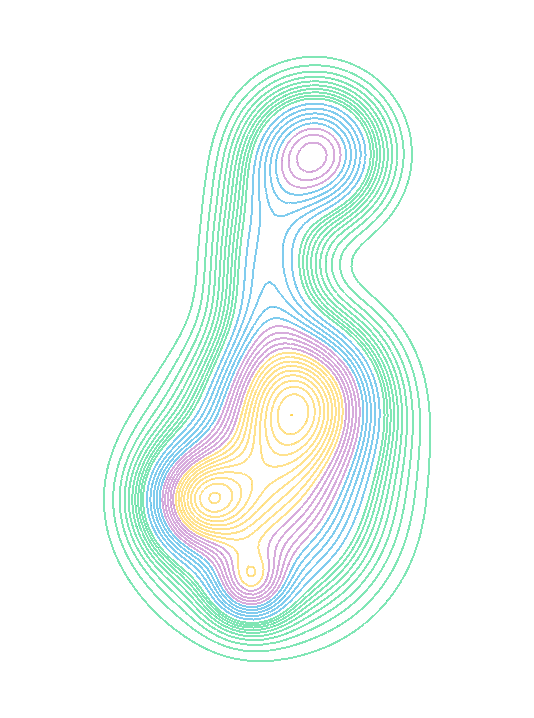
\includegraphics[trim=100 25 75 0, clip, angle=280, scale=0.25]{scripts/figures/scalar_contour.png}
  
\includegraphics[trim=200 200 200 200, clip, width=0.5\textwidth]{scripts/figures/surf/side.png}
  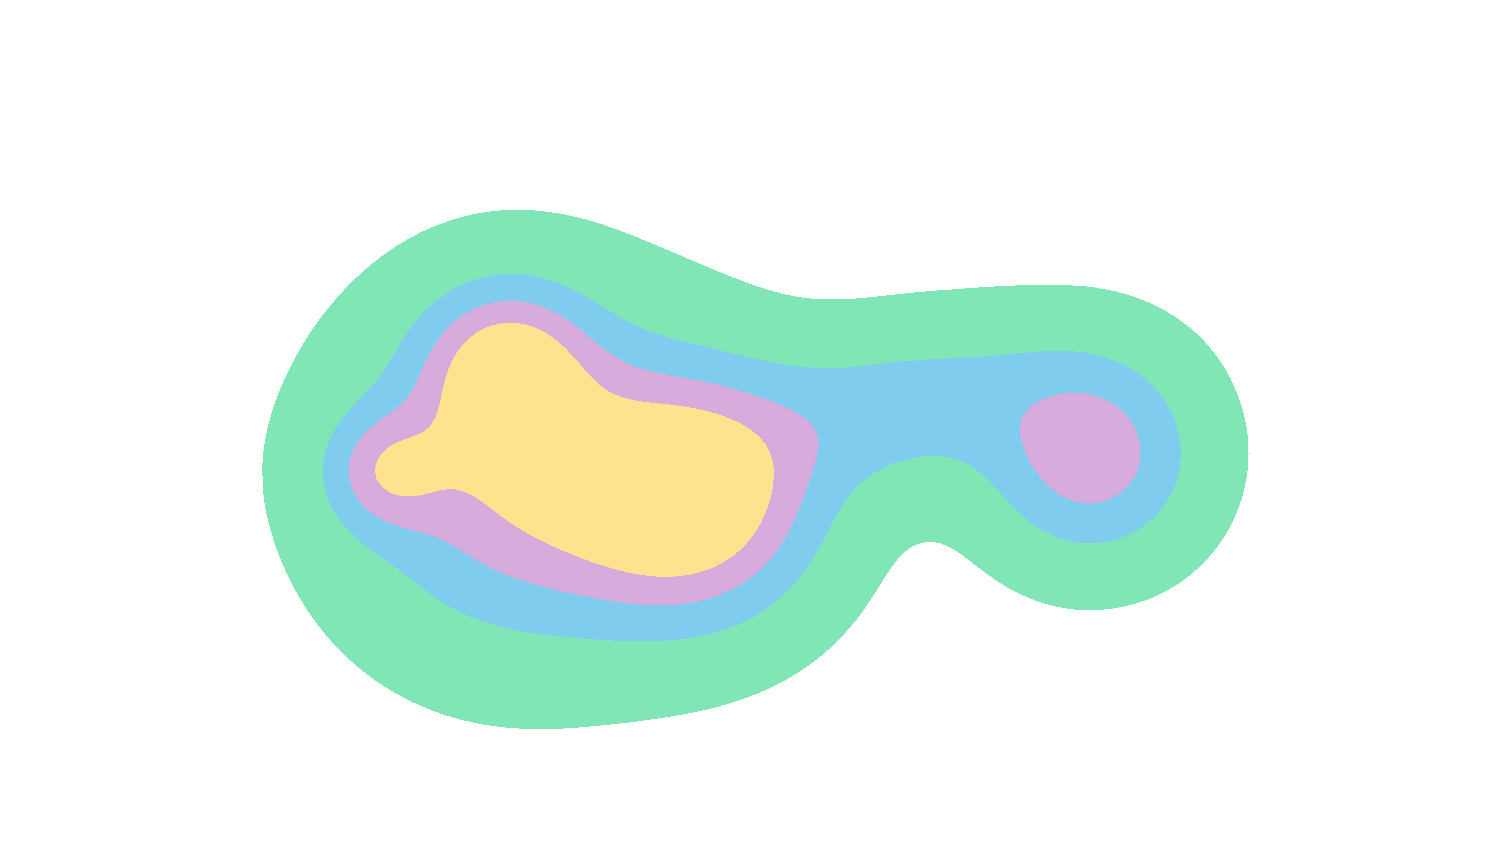
\includegraphics[trim=200 0 200 200, clip, width=0.3\textwidth]{scripts/figures/surf/top.png}
  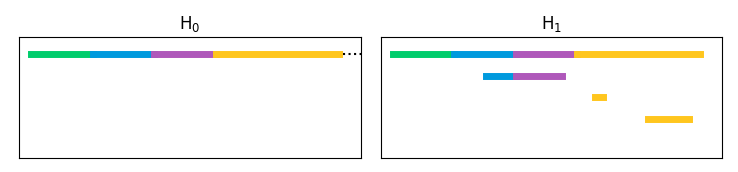
\includegraphics[scale=0.75]{scripts/figures/scalar_barcode_true.png}
  % \includegraphics[trim=0 310 270 0, clip, scale=0.8]{scripts/figures/scalar_restricted.png}
  % \includegraphics[scale=0.55]{scripts/figures/scalar_barcode_super_0.png}
  % \includegraphics[scale=0.55]{scripts/figures/scalar_barcode_sub_1.png}
\end{figure}


\clearpage
\section{Background}

\subsection{Geometry and Topology}
  % !TeX root = ../../main.tex

% \subsection{Topology and Geometry}

\paragraph{Separation}

Let $X$ be a topological space.
A \textbf{separation} of $X$ is a pair $A, B$ of disjoint, nonempty, open subsets of $X$ whose union is $X$.
The space $X$ is said to be \textbf{connected} if there does not exist a separation of $X$.

Note that the sets $A, B$ that form a separation of $X$ are both open and closed in $X$.
For a subspace $Y$ of $X$ we will denote the interior and closure of a set $U$ in $Y$ with $\intr_Y(U)$ and $\cl_Y(U)$.
If $Y$ is a subspace of $X$, a separation of $Y$ is a pair of disjoint, nonempty sets $A, B$ whose union is $Y$, neither of which contains a limit point of the other.
The space $Y$ is connected if there exists no separation of $Y$ (Munkres~\cite{munkres00topology}, Lemma 23.1).

% If $A, B$ is a separation of a subspace $Y$ of $X$ then $A, B$ are both open and closed in $Y$, but not necessarily $X$.
% The condition that neither $A$ nor $B$ contains a limit point of the other requires that $\cl_X(A)\cap B = \emptyset$ and $A\cap \cl_X(B) =\emptyset$ where $\cl_Y(A) = A$ and $\cl_Y(B) = B$.

% \begin{definition}[Components (Munkres~\cite{munkres00topology})]
%   Given $X$, define an equivalence relation on $X$ by setting $x\sim y$ if there is a connected subspace of $X$ containing both $x$ and $y$.
%   The equivalence class are called the \textbf{components} (or ``connected components'') of $X$.
% \end{definition}

For a disconnected topological space $X$ let $X_1, X_2, \ldots$ denote its path-connected components.
For $A\subseteq X$ let $A_i = A\cap X_i$ denote the component of $A$ in $X_i$.

\begin{definition}[Separating Set]
  Let $X$ be a (possibly disconnected) topological space and $V\subset X$.
  $V$ \textbf{separates $X$ with a pair $(A, B)$} if $(A_i, B_i)$ is a separation of $X_i\setminus V_i$ for all $i$.
\end{definition}

If $V$ separates $X$ with a pair $(A, B)$ then $X = A\sqcup V\sqcup B$.
Note that while $A$ and $B$ are both open and closed in $X\setminus V$, each component $X_i = A_i\sqcup V_i\sqcup B_i$ is connected.
Therefore, if $V$ separates $X$ with a pair $(A, B)$, we require that $\cl_X(A)\cap B = \emptyset$ and $A\cap \cl_X(B) = \emptyset$.
% If $V$ is an open set in $X$ then $A$ and $B$ are closed in $X$, therefore $\cl_X(A)\cap B = \emptyset$ and $A\cap \cl_X(B) = \emptyset$.
% Otherwise, if $V$ is closed in $X$, then $A$ and $B$ are open in $X$.

For $A\subseteq X$ let $\overline{A} := X\setminus A$ denote the complement of $A$ in $X$.

\paragraph{Metric Spaces}

Let $(X,\dist)$ be a metric space where $\dist(x, y)$ denotes the distance between points $x,y\in X$.
For $P\subset X$ and $x\in X$ let $\dist_P(x) = \displaystyle\min_{p\in P}\dist(p, x)$ denote the distance from $x$ to the set $P$.
We will use open metric balls $\ball^\e(x) = \{y\in X\mid \dist(x, y) < \e\}$ and offsets $P^\e = \{x\in X\mid \dist_P(x) < \e\}.$
A real-valued function $f$ on $X$ is $c$-Lipschitz if for all $x,y\in X$ we have
\[
  |f(x) - f(y)| \le c \dist(x,y).
\]

A metric ball is said to be \textbf{strongly convex} if for each pair of points $y,z$ in its closure there exists a unique shortest path in $X$ between $y$ and $z$ whose interior is contained in the metric ball.
For $x\in X$ let $\varrho_X(x)$ be the supremum of the radii $\e$ such that $\ball^\e(x)$ is strongly convex.
The \textbf{strong convexity radius} of $X$ is defined as
\[ \varrho_X := \inf_{x\in X} \varrho_X(x).\]
Note that this value is positive for compact $X$.
Importantly, strongly convex sets are contractible, and intersections of stronly convex sets are also strongly convex~\cite{chazal09analysis}.
Given a subspace $D\subseteq X$ let $\ball_D^\e(x)$ denote the open ball $D\cap \ball_X^\e(x)$ in the subspace topology and $\varrho_D$ denote the strong convexity radius of $D$.


\subsection{Simplicial Complexes}\label{sec:complexes}
  % !TeX root = ../../main.tex

% \subsection{Simplicial Complexes}\label{sec:complexes}

A \textbf{simplicial complex} $K$ is a collection of subsets, called \textbf{simplices}, of a vertex set $V$ such that for all $\sigma\in K$ and $\tau\subset\sigma$ it must follow that $\tau\in K$.
The \textbf{dimension} of a simplex $\sigma\in K$ is defined as $\dim(\sigma) := |\sigma|-1$ where $|\cdot|$ denotes set cardinality.
The dimension of a simplicial complex $K$ is the maximum dimension of any simplex in $K$.
That is, a graph is a 1-dimensional simplicial complex in which vertices and edges are 0 and 1-dimensional simplices, respectively.

% \figblock{%
% \begin{figure}[htbp]
% \centering
%     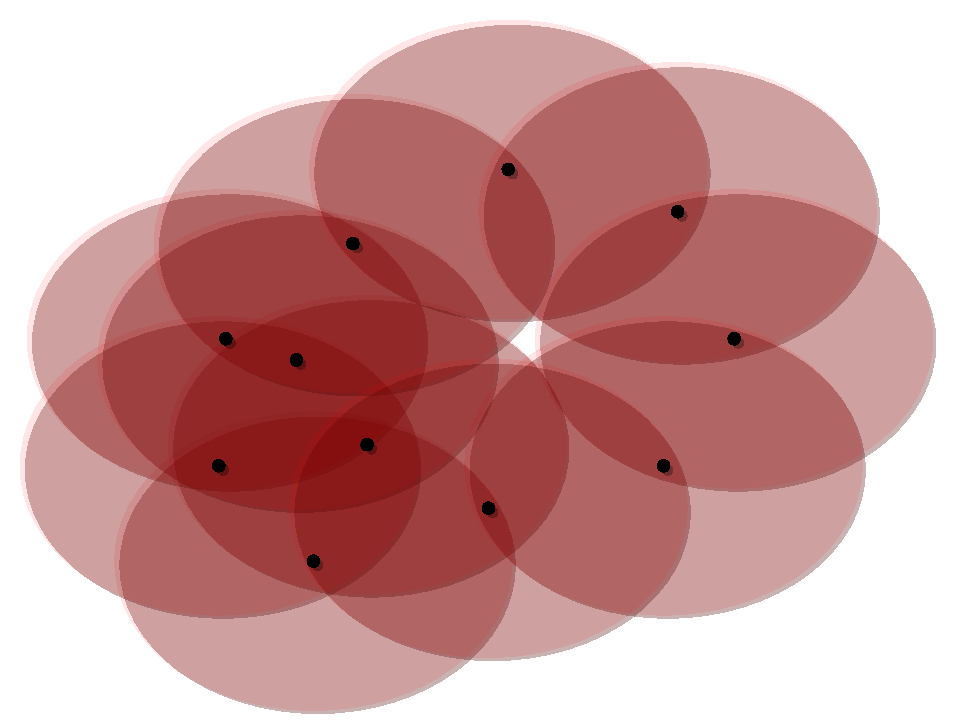
\includegraphics[scale=0.33]{figures/holes_cover.pdf}
%     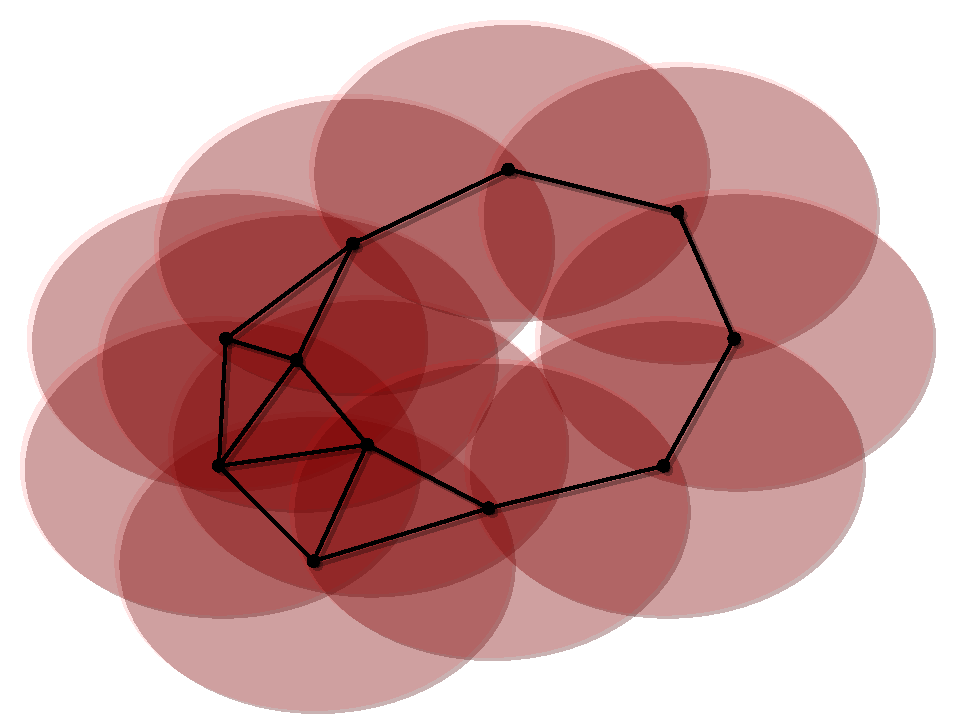
\includegraphics[scale=0.33]{figures/holes_edges.pdf}
%     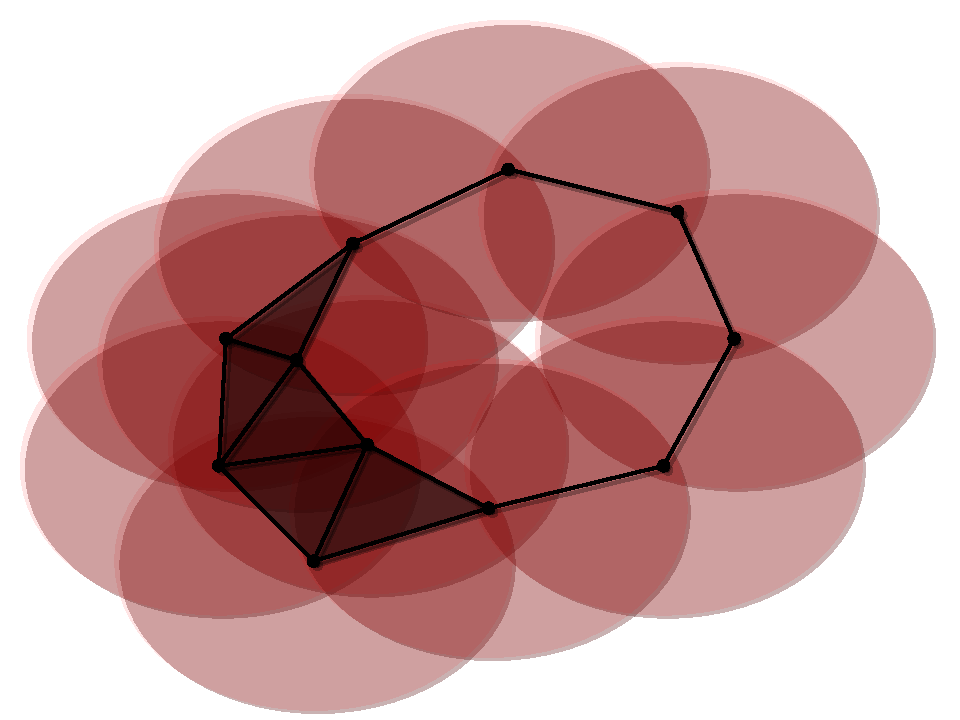
\includegraphics[scale=0.33]{figures/holes_complex.pdf}
%      \caption{(Left) The coverage regions of a collection of points $P$ at some scale $\alpha$.
%             (Middle) The neighborhood graph with edges for each pair of points within pairwise distance $\alpha$.
%             (Right) If we attempt to fill cycles in the graph with triangles identify a cycle that cannot be filled which reflects a gap in coverage}
%      \label{fig:holes}
% \end{figure}}

It is natural to think of a $k$-dimensional simplicial complex as the generalization of an undirected graph consisting of vertices and edges, collections of at most 2 vertices, to collections of sets of at most $k-1$ vertices.
% Just as we have defined a hole in our graph $G$ as a cycle that cannot be filled with triangles, we define a $k$-dimensinal hole in a simplicial complex as a $k$-cycle that cannot be filled with $(k+1)$-simplices.
% In the next section we will formally define $k$-cycles and introduce simplicial homology as a tool for identifying when and which cycles cannot be filled.

\paragraph{Coordinate-free Communication}
% In a coordinate-free sensor network each sensor, represented by a point in $P$, is capable of detecting nodes which are sufficiently ``close.''
% That is, there is some radius of communication $\delta > 0$ such that two nodes $p, q\in P$ such that $\dist(p, q) \leq\delta$ are capable of communication.
% Note that, although sensors can communicate within this distance they are not able to measure the distance itself.

Let $P$ be a finite collection of points in a subspace $D$ of some (unknown) metric space $X$.
In a coordinate-free setting we provided with some notion of connectivity between the points in $P$ but not their precise locations, nor the distances between them.
For example, in coordinate-free sensor networks each sensor is represented by a point in $P$ and there is some distance $\delta > 0$ that sensors can communicate within, but not able measure.

With this limited capability we can construct an undirected graph $G=(V, E)$ with vertices $V=P$ and edges $E = \{\{p, q\}\subset P\mid \dist(p,q)\leq\delta\}$.
Let $K$ be a simplicial complex with 0-simplices $\{v\}$ for all $p\in P$, 1-simpices $\{u, v\}\subset P$ for each edge in $E$, and 2-simplices $\{u,v,w\}\subset P$ whenever $\{\{\{u,v\},\{v,w\},\{u,w\}\}\subset E$.
This particular simplicial complex is known as the Vietoris-Rips complex.
It is also an example of a clique complex, where the simplices are the complete subgraphs (or cliques) in a given graph.

Formally, the \textbf{(Vietoris-)Rips complex} is defined for a set $P$ at scale $\e > 0$ as
\[ \rips^\e(P) = \left\{\sigma \subseteq P\mid \forall p,q\in\sigma,\ \dist(p, q)\leq \e\right\}. \]
For a pair $(P, Q)$ we will write $\rips^\e(P,Q) := (\rips^\e(P), \rips^\e(Q))$ to denote the corresponding pair of rips complexes.

\paragraph{Coverage}
% In order to determine coverage we must at least assert that the coverage domain spanned by the points in $P$ does not contain any holes.
% Assuming the coverage radius of our sensors is equal to their communication radius $\delta$ we may define a hole in coverage as a cycle that cannot be ``filled'' with triangles (see Fig.~\ref{fig:holes}).

% \figblock{%
% \begin{figure}[htbp]
% \centering
%     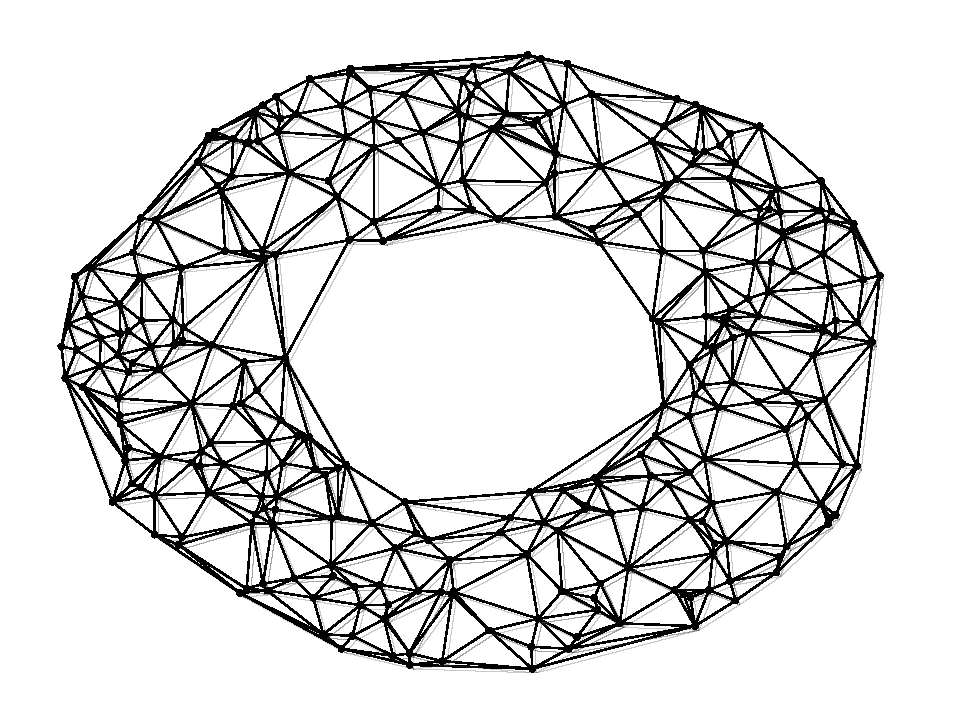
\includegraphics[scale=0.33]{figures/boundary_graph.pdf}
%     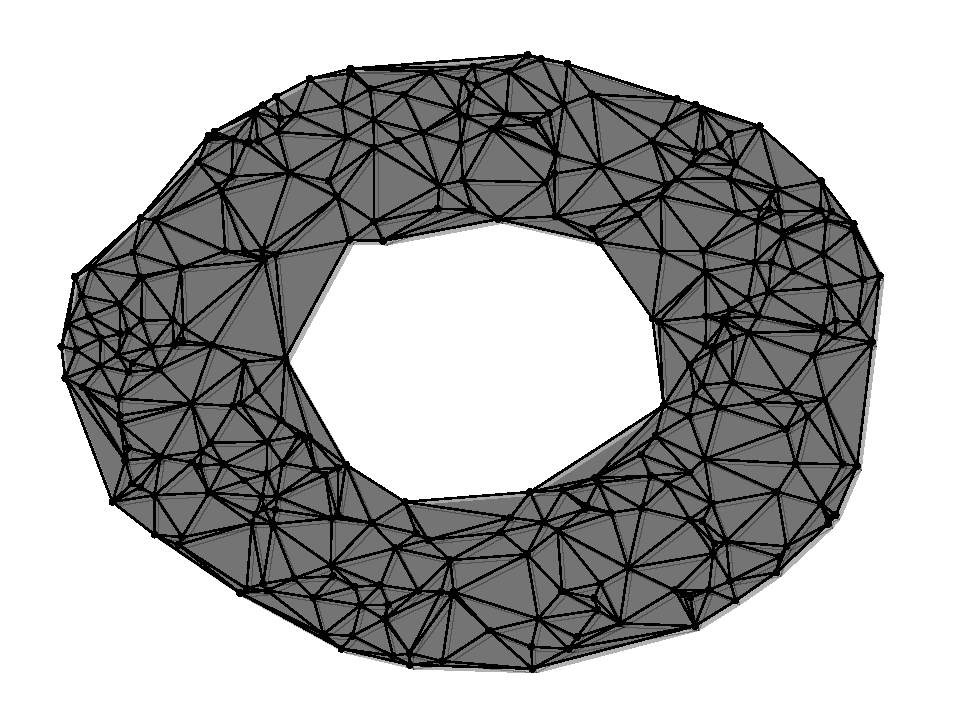
\includegraphics[scale=0.33]{figures/boundary_complex.pdf}
%     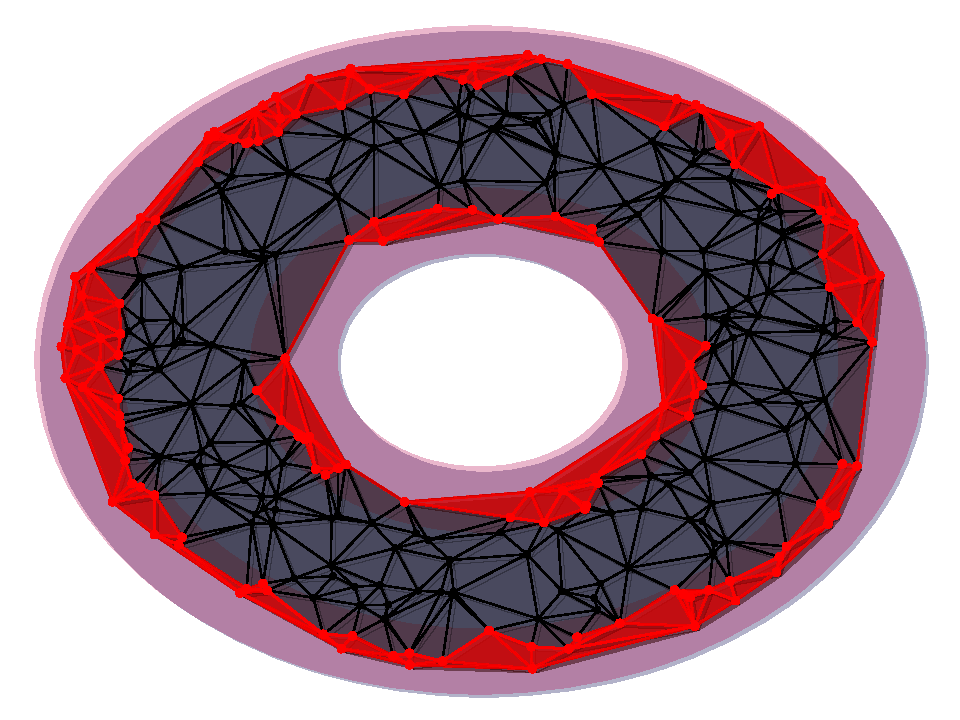
\includegraphics[scale=0.33]{figures/boundary_complex_domain_fence.pdf}
%     % 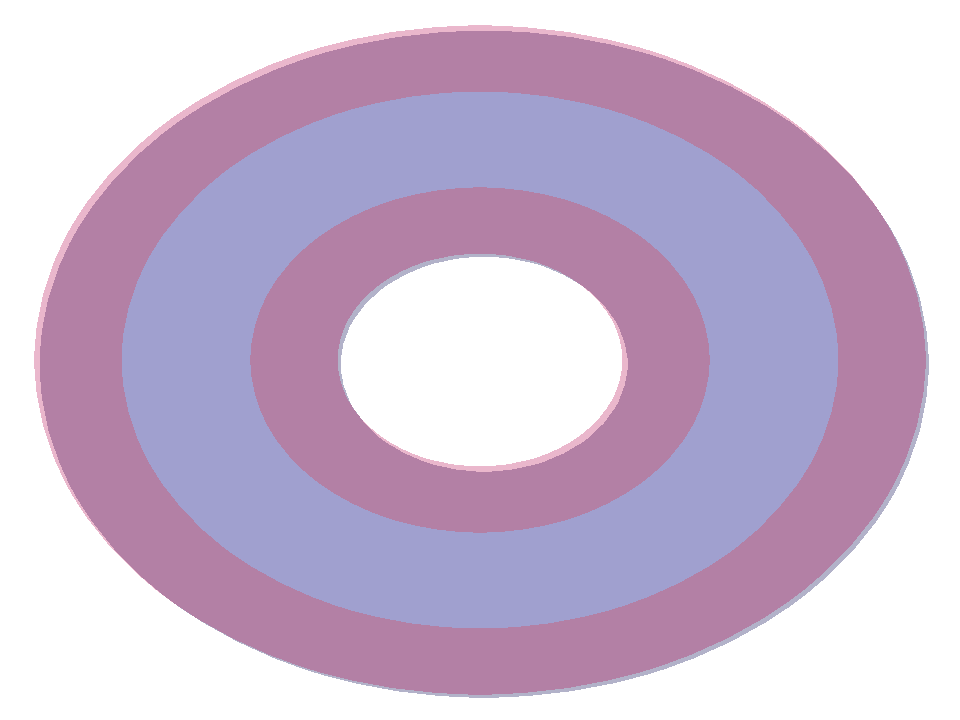
\includegraphics[scale=0.24]{figures/boundary_domain.pdf}
%      \caption{(Left) The neighborhood graph of a sensor network with a large ``hole''.
%             (Middle) A 2-dimensional simplicial complex with no gaps in coverage, but an unfilled cycle.
%             (Right) By allowing nodes to identify the boundary (in red) we can confirm coverage of complex domains.}
%      \label{fig:boundary1}
%  \end{figure}}

If a collection of points $P$ covers $D$ at scale $\e$, that is, $D\subseteq P^\e$, the topology of the domain is reflected in $\rips^\e(P)$.
However, as we will see, this does not necessarily give a tight bound on the minimum radius for coverage.
In fact, if the coverage region of of a sensor network at scale $\e$ has no gaps, then the minimum coverage radius required is a constant factor smaller than $\e$.
This point is made clear by an interleaving of the Rips with another simplicial complex known as the \v Cech complex.

The \textbf{\v Cech complex} of a finite collection of points $P$ at scale $\e > 0$ is defined
  \[ \cech_\e(P) = \left\{\sigma \subseteq P\mid \bigcap_{p\in \sigma}\ball_\e(p)\neq \emptyset \right\}. \]
The \v Cech and Rips complexes of a finite metric space are closely related by a result that follows from Jung's Theorem~\cite{jung01uber} relating the diameter of a point set $P$ and the radius of the minimum enclosing ball:
\[\cech^{\e/\jungd}(P)\subseteq\rips^\e(P)\subseteq\cech^\e(P)\subseteq\rips^{\jungd\e}(P),\]
where the constant $\jungd = \sqrt{\frac{2d}{d+1}}$ (see~\cite{buchet15efficient}).

The \v Cech complex is a special case of a more general construction known as the \textbf{nerve} $\N(\cU)$ of a collection of sets $\cU = \{U_i\}_{i\in I}$, where $I$ is any indexing set.
The nerve of $\cU$ is defined as the simplicial complex with vertex set $I$ such that $\sigma\subseteq I$ is a simplex if and only if
\[
  \bigcap_{i\in \sigma} U_i\neq \emptyset.
\]
The collection $\cU$ is a \textbf{good cover} if for each $\sigma\subset I$ the set $\bigcap_{i\in\sigma} U_i$ is contractible or empty.
The \textbf{Nerve Theorem} states that if $\cU$ is a good cover then its nerve $\N(\cU)$ is homotopy equivalent to $\bigcup_{i\in I} U_i$.

That is, for a set of points $P\subset D$ such that $cU = \{\ball^\e(p)\mid p\in P\}$ is a good cover the nerve $\N(\cU)$ is homotopy equivalent to $P^\e = \bigcup_{p\in P} \ball_\e(p)$.
Note that whenever $\varrho_D > \e$ all open balls $\ball^\e_D(p)$ are either empty or contractible.
So $\cU$ is a good cover and the inclusion $\cech^\e(P)\hookrightarrow P^\e$ is a homotopy equivalence.

%
%
\subsection{Homology}\label{sec:homology}
  % !TeX root = ../../main.tex

For a simplicial complex $K$ let $C_k(K)$ denote the vector space over a field $\F$ consisting of linear combinations of $k$-simplices in $K$ known as \textbf{$k$-chains}.
These vector spaces are connected by \textbf{boundary maps} $\partial_k:C_k(K)\to C_{k-1}(K)$ which are linear transformations taking basis elements of $C_k(K)$ to the abstract sum of basis $(k-1)$-simplex faces.
The collection of chains and boundary maps forms a sequence of vector spaces known as the \textbf{chain complex} of $K$.

An important property of the boundary maps $\partial_k$ is that the composition of subsequent boundary maps is zero.
That is, $\partial_k\circ\partial_{k-1} = 0$ for all $k$.
As a result the image of $\partial_{k+1}$, denoted $\im~\partial_{k+1} = \{\partial_{k+1}c\mid c\in C_{k+1}(K)$ is a subspace of the kernel, $\ker~\partial_k = \{c\in C_k(K)\mid \partial_k c = 0\}$, of $\partial_k$.
A \textbf{$k$-cycle} of $\C$ is a $k$-chain with empty boundary---an element of $\ker~\partial_k$.
Two cycles in $\ker~\partial_k$ are said to be \textbf{homologous} if they differ by an element of $\im~\partial_{k+1}$.
The \textbf{$k$th homology groups} of $K$ is the quotient group $\hom_k(K) = \ker~\partial_k/\im~\partial_{k+1}$.
Elements of $\hom_k(K)$ are equivalence classes $[x]$ of homologous $k$ cycles.
That is, if $[x] = [y]$ for any $x,y\in C_k(K)$ then $x = y +\partial_{k+1}z$ for some $z\in C_{k+1}(K)$.


% The rank of a homology group is of particular importance and is known as the \textbf{Betti number} $\beta_k = \rank~ \hom_k(K)$.
% These topological invariants can be thought of as counting the number of $k$-dimensional ``holes'' in a topological space, where $0$-dimensional holes are connected components, $1$-dimensional holes are loops, $2$-dimensional holes are voids, and so on.
% Note that this is the same notion which motivated our use of simplicial complexes for determining coverage---a $1$-dimensional hole exists if a gap in a neighborhood graph cannot be filled by triangles.

While we have chosen to define simplicial homology for ease of exposition we will primarily be using singular homology over a field $\F$ so that the homology groups $\hom_k(X)$ of a topological space $X$ are vector spaces.
For a full treatment of both singular and simplicial homology see Hatcher~\cite{hatcher01}.

\paragraph{Relative Homology}

Let $(X, Y)$ be a pair of topological spaces (or pair of simplicial complexes).
The relative chain groups $C_k(X, Y) = C_k(X) / C_k(Y)$ consist of equivalence classes of chains in $C_k(X)$ that differ by chains in $C_k(Y)$.
We note that the boundary map $\partial_k$ on $C_k(X)$ induces a boundary map on the quotient $C_k(X, Y)$ such that $\partial_k(y) = 0$ for all $y\in C_k(Y)$.

The \textbf{$k$th relative homology group} $\hom_k(X, Y)$ consists of homology classes of relative cycles---chains in $C_k(X)$ whose boundaries vanish or lie in $Y$.
That is, a relative $k$-cycle can either be a cycle in $C_k(X)$ or a chain in $C_k(X)$ with a boundary in $C_{k-1}(Y)$.
We will make extensive use the \textbf{excision} axiom of homology which states that for any $A\subset Y$ such that $\cl_X(A)\subseteq \intr_X(Y)$ the inclusion of pairs $(X\setminus A, Y\setminus A)\hookrightarrow (X, Y)$ induces isomorphisms on relative homology groups $\hom_k(X\setminus A, Y\setminus A)\cong\hom_k(X, Y)$.

\paragraph{Exact Sequences}

A sequence $A\xrightarrow{i} B\xrightarrow{j} C$ is said to be \textbf{exact} if $\im~i = \ker~j$.
An exact sequence $0\to A\to B\to C\to 0$ is said to be \textbf{short exact}.
In general, any exact sequence $\ldots\to A\to B\to C\to\ldots$ is referred to as a long exact sequence.

For any pair of topological spaces $(X, Y)$ the \textbf{long exact sequence of the pair} is the exact sequence
\[ \ldots\to\hom_{k+1}(X, Y)\xrightarrow{\partial_{k+1}} \hom_k(Y)\xrightarrow{i_k} \hom_k(X)\xrightarrow{j_k}\hom_k(X, Y)\xrightarrow{\partial_k}\hom_{k-1}(Y)\to\ldots.\]
Here the map $\partial_k$ is the connecting homomorphism which is induced by the boundary map on $C_k(X, Y)$.

% section homology (end)

%
\subsection{Persistence Modules}
  % !TeX root = ../../main.tex

\begin{definition}[Persistence Module]
  A \textbf{persistence module} $\S$ over $\R$ is an indexed family of vector spaces $\{S_\alpha\}$ and linear maps $\{s_\alpha^\beta : S_\alpha\to S_\beta\}$ such that $s^\gamma_\beta\circ s_\alpha^\beta = s_\alpha^\gamma$ whenever $\alpha\leq\beta\leq\gamma$ and $s_\alpha^\alpha$ is the identity on $S_\alpha$.
\end{definition}

% For a persistence module $\S$ we will also use $S[\alpha]$ to denote the vector space $S_\alpha$ and $s[\alpha,\beta]$ to denote the linear maps $s_\alpha^\beta$ when additional notation is required.

\begin{definition}[Persistence Module Homomorphism]
  A \textbf{homomorphism} $\Lambda$ between two $\R$-persistence modules $\S, \T$ is a collection of linear maps $\{\lambda_\alpha : S_\alpha\to T_\alpha\}$ such that the following diagram commutes for all $\alpha\leq\beta$.
  \begin{equation}\label{dgm:homomorphism}
    \begin{tikzcd}
      S_\alpha\arrow{r}{s_\alpha^\beta}\arrow{d}{\lambda_\alpha} &
      S_\beta\arrow{d}{\lambda_\beta}\\
      %
      T_\alpha\arrow{r}{t_\alpha^\beta} &
      T_\beta
  \end{tikzcd}\end{equation}
  The space of homomorphisms from $\S$ to $\T$ will be denoted $\Hom(\S, \T)$.
\end{definition}

\begin{definition}[Shifted Homomorphism]
  A \textbf{homomorphism of degree $\delta$} is a collection $F$ of linear maps $f_\alpha : U_\alpha\to S_{\alpha+\delta}$ such that the following diagram commutes for all $\alpha\leq\beta$.

  \begin{equation}\label{dgm:shifted_homomorphism}
    \begin{tikzcd}
      U_\alpha\arrow{r}{u_\alpha^\beta}\arrow{d}{f_\alpha} &
      U_\beta\arrow{d}{f_\beta}\\
      %
      S_{\alpha+\delta}\arrow{r}{s_{\alpha+\delta}^{\beta+\delta}} &
      S_{\beta +\delta}
  \end{tikzcd}\end{equation}
  The space of homomorphisms of degree $\delta$ from $\U$ to $\S$ will be denoted $\Hom^\delta(\U, \S)$.
\end{definition}

Noting that $\Hom^\delta(\U,\V)\subseteq\Hom^{\delta'}(\U,\V)$ for all $0\leq\delta\leq\delta'$ we will define particular shifted homomorphisms with the assumption that $\Hom^\delta(\U,\V) = \Hom(\U,\V)$ for $\delta = 0$.
For $\Gamma\in\Hom(\U,\V)$ let $\Gamma[\delta]\in\Hom^\delta(\U,\V)$ denote the homomorphism of degree $\delta$ defined as the family of linear maps
\[\{\gamma_\alpha[\delta] := v_\alpha^{\alpha+\delta}\circ \gamma_\alpha : U_\alpha\to V_{\alpha+\delta}\}.\]

% Using our alternative notation we will write
% \[\gamma[\alpha;\delta] := v[\alpha,\alpha+\delta]\circ\gamma[\alpha] : U[\alpha]\to V[\alpha+\delta]\]
% to denote a map $\gamma_\alpha[\delta]$ of $\Gamma[\delta]$.

% \begin{lemma}\label{lem:trans_shift}
%   If $F\in \Hom^\delta(\U,\S)$ and $F'\in\Hom^{\delta'}(\S,\S')$ then $F'\circ F\in\Hom^{\delta+\delta'}(\U,\S')$.
% \end{lemma}
% \begin{proof}
%   Because $F'\in \Hom^{\delta'}(\S,\S')$ we have $f_{\beta}'\circ s_\alpha^\beta = {s_{\alpha+\delta'}^{\beta+\delta'}}'\circ f_{\alpha+\delta'}'$ for all $\alpha\leq\beta$.
%   Because $F\in\Hom^\delta(\U,\S)$ we have $f_{\beta-\delta}\circ u_{\alpha-\delta}^{\beta-\delta} = s_\alpha^\beta\circ f_{\alpha-\delta}$ for all $\alpha\leq\beta$.
%   So
%   \begin{align*}
%     f_{\beta}'\circ (f_{\beta-\delta}\circ u_{\alpha-\delta}^{\beta-\delta})
%       &= (f_{\beta}'\circ s_\alpha^\beta)\circ f_{\alpha-\delta}\\
%       &= {s_{\alpha+\delta'}^{\beta+\delta'}}'\circ f_{\alpha+\delta'}'\circ f_{\alpha-\delta}
%   \end{align*}
%   so $F'\circ F\in\Hom^{\delta+\delta'}(\U,\S')$.
% \end{proof}

\begin{definition}[Interleaving]
  Two persistence modules $\U$ and $\S$ are \textbf{$\delta$-interleaved} if there exist homomorphisms $F\in\Hom^\delta(\U, \S)$ and $G \in\Hom^\delta(\S,\U)$ such that the following diagrams commute for all $\alpha$.

  \begin{minipage}{0.45\textwidth}
  \begin{equation}\label{dgm:interleaving1}
    \begin{tikzcd}
      U_{\alpha-\delta}\arrow{rr}{u_{\alpha-\delta}^{\alpha+\delta}}\arrow{dr}{f_{\alpha-\delta}} & &
      U_{\alpha+\delta}\\
      %
      & S_{\alpha}\arrow{ur}{g_\alpha} &
  \end{tikzcd}\end{equation}
  \end{minipage}
  \begin{minipage}{0.45\textwidth}
  \begin{equation}\label{dgm:interleaving2}
    \begin{tikzcd}
      & U_{\alpha}\arrow{dr}{f_\alpha} &\\
      %
      S_{\alpha-\delta}\arrow{rr}{s_{\alpha-\delta}^{\alpha+\delta}}\arrow{ur}{g_{\alpha-\delta}} & &
      S_{\alpha+\delta}
  \end{tikzcd}\end{equation}
  \end{minipage}
\end{definition}

% \subsubsection{Interval Modules}
\paragraph{Interval Modules}

For an interval $I = [s,t)\subseteq \R$ let $I_+ := [t,\infty)$ and $I_- := (-\infty, s]$.
For $\alpha\leq\beta\in\R$ let
\[ F_\alpha^I := \begin{cases} \FF&\text{ if } \alpha\in I\\ 0 &\text{otherwise,}\end{cases}\ \text{ and }\ \ f_{\alpha,\beta}^I := \begin{cases} \id_\FF&\text{ if } \alpha,\beta\in I\\ 0&\text{otherwise.}\end{cases}.\]
An \textbf{interval module} is a persistence module $\FF^I$ defined to be the family of vector spaces $\{F_\alpha^I\}_{\alpha\in\R}$ along with linear maps $\{f_{\alpha,\beta}^I : F_\alpha^I\to F_\beta^I\}_{\alpha\leq\beta}$.

A \textbf{interval decomposition} of a persistence module $\S$ a collection $\I$ of interval $I\subseteq\R$ such that
\[ \S = \bigoplus_{I\in \I} \FF^I. \]
If such a decomposition exists $\S$ is said to be \textbf{decomposable}.

% \subsection{}
%
% \begin{definition}[Weak Interleaving]
%   For $I\in\Hom^{2\delta}(\U,\V)$ a pair $(F, M)\in \Hom^\delta(\U,\S)\times\Hom^\delta(\S,\V)$ is a \textbf{weak $\delta$-interleaving} of $I$ with $\S$ if $I = M\circ F$.
%   If $J\in\Hom^{\delta'}(\S,\T)$ and $(F,N)\in\Hom^\delta(\U,\S)\times\Hom^\delta(\T,\V)$ is a weak $\delta$-interleaving of $I$ with $J$ if $I = N\circ J\circ F$.
% \end{definition}
%
% \begin{lemma}\label{lem:left}
%   Let $I\in\Hom^{4\delta}(\U,\V)$, $J\in\Hom^{2\delta}(\S,\T)$ and suppose $(F, N)\in\Hom^{\delta}(\U,\S)\times\Hom^\delta(\T,\V)$ is a weak $\delta$-interleaving of $I$ with $J$.
%
%   If $(F', M')\in\Hom^\delta(\S,\S')\times\Hom^\delta(\S',\T)$ is a weak $\delta$-interleaving of $J$ with $\S'$ then
%   \[(F'\circ F, N\circ M')\in\Hom^{2\delta}(\U,\S')\times \Hom^{2\delta}(\S',\V)\]
%   is a weak $2\delta$-interleaving of $I$ with $\S'$.
% \end{lemma}
% \begin{proof}
%   By Lemma~\ref{lem:trans_shift} we have $F'\circ F\in\Hom^{2\delta}(\U,\S')$ and $N\circ M'\in \Hom^{2\delta}(\S',\V)$.
%   If $(F', M')$ is a weak $\delta$-interleaving of $J$ with $\S'$ then $J = M'\circ F'$.
%   By our hypothesis that $(F, N)$ is a weak $\delta$-interleaving of $I$ with $J$
%   \[ I = N\circ J\circ F = (N\circ M')\circ (F'\circ F).\]
%   We may therefore conclude that $(F'\circ F, N\circ M')\in\Hom^{2\delta}(\U,\S')\times \Hom^{2\delta}(\S',\V)$ is a weak $2\delta$-interleaving of $I$ with $\S'$.
% \end{proof}
%
% \begin{lemma}\label{lem:right}
%   Let $I\in\Hom^{2\delta}(\U,\V)$, $I'\in\Hom^{4\delta}(\U',\V')$ and suppose $(F, M)\in\Hom^\delta(\U,\S)\times\Hom^\delta(\S,\V)$ is a weak $\delta$-interleaving of $I$ with $\S$.
%
%   If $(F',N')\in\Hom^\delta(\U',\U)\times\Hom^\delta(\V,\V')$ is a weak $\delta$-interleaving of $I'$ with $I$ then
%   \[(F\circ F', N'\circ M)\in\Hom^{2\delta}(\U',\S)\times\Hom^{2\delta}(\S,\V')\]
%   is a weak $2\delta$-interleaving of $I'$ with $\S$.
% \end{lemma}
% \begin{proof}
%   By Lemma~\ref{lem:trans_shift} we have $F\circ F'\in \Hom^{2\delta}(\U',\S)$ and $N'\circ M\in \Hom^{2\delta}(\S,\V')$.
%   By our hypothesis that $(F, M)$ is a weak $\delta$-interleaving of $I$ with $\S$ we know $I = M\circ F$.
%   If $(F',N')$ is a weak $\delta$-interleaving of $I'$ with $I$ then $I' = N'\circ I\circ F'$.
%   \[ I' = N'\circ I\circ F' = (N'\circ M)\circ (F\circ F').\]
%   We may therefore conclude that $(F\circ F', N'\circ M)\in\Hom^{2\delta}(\U',\S)\times\Hom^{2\delta}(\S,\V')$ is a weak $2\delta$-interleaving of $I'$ with $\S$.
% \end{proof}
%

%
\subsection{Persistent Homology}
  % !TeX root = ../../main.tex

% We are interested in a particular persistence module that can be obtained by applying homology as a functor from the category of topological spaces to the category of abelian groups.
Given a topological space $X$ a \textbf{filtration} of $X$ is a sequence of subspaces $\emptyset = X_0\subseteq X_1\subseteq\ldots\subseteq X_n = X$.
The \textbf{$k$th persistent homology module} of a filtration $\{X_i\}_{i\in I}$ over an indexing set $I$ is the persistence module consisting of vector spaces $\hom_k(X_i)$ and linear maps $\hom_k(X_i)\to \hom_k(X_j)$ induced by inclusion for $i\leq j$.
Similarly, given a pair $(X,Y)$ and filtrations $\{X_i\}_{i\in I}$ and $\{Y_i\}_{i\in I}$ such that $Y_i\subseteq X_i$ for all $i\in I$ the $k$th persistent relative homology module is the persistence module of vector spaces $\hom_k(X_i, Y_i)$ and linear maps $\hom_k(X_i, Y_i)\to\hom_k(X_j, Y_j)$ induced by inclusions for all $i\leq j$.

Given a function $f: X\to \R$ we can define a filtration known as \textbf{sublevel set filtration} as a sequence of sublevel sets $\{f^{-1}((-\infty, \alpha])\}_{\alpha\in\R}$ where $f^{-1}((-\infty, \alpha]) := \{x\in X\mid f(x)\leq\alpha\}$.
The superlevel set filtration of $f$ is similarly defined $\{f^{-1}([\alpha,\infty))\}_{\alpha\in\R}$.
% The persistent homology of the sub(or super)-levelset filtration is typically referred to as the persistent homology of $f$.

The persistent homology of a filtration encodes the homology of a space as it changes monotonically in some way.
In the case of the sublevel set filtration, this is the change in homological structure of subspaces of $X$ that map to intervals $(-\infty,\alpha]$ as $\alpha$ increases.
These changes are referred to as the birth and death of a \emph{feature} in some dimension---homology classes that \emph{persist} over an interval $[b, d)\subset\R$.
This information can be summarized by a \textbf{persistence diagram} or \textbf{barcode} which visualizes these features either as pairs of points $(b, d)\in\R^2$, or as intervals $[b, d)\subset\R$.

There is a metric on the space of persistence diagrams known as the \textbf{bottleneck distance}.
In most cases we are concerned with, the bottleneck distance is equal to the interleaving distance---that is, if two persistent homology modules are $\delta$-interleaved then the bottleneck distance between their associated diagrams is $\delta$.



\clearpage
\section{The Topological Coverage Criterion (TCC)}
% !TeX root = ../../main.tex

% A collection of sensors can be verified as covering a domain if
% \begin{enumerate}
%     \item[a.] the boundary of the domain is adequately covered,
%     \item[b.] the interior of the
% \end{enumerate}
% Condition (b) relies on condition (a) in order to provide a topological condition that is necessary but not sufficient.
% Given (a) we can confirm coverage by checking if the balloon has been punctured simply by checking the dimension of the top-dimensional relative homology of the sample.
%
% Adequate coverage of the boundary can be broken into two parts.
% First, we require that the sampled boundary is sufficiently simple in order to ensure our condition cannot produce false positives.
% This is achieved by using what we refer to as \emph{short-filtrations}: applying one step of persistence in order to de-noise the data.
% By testing our network at two scales we can ensure no spurious features are present in the boundary which may contribute to false positives.
% % We also note that these short-filtrations are employed in the analysis of scalar fields as well.
%
% Secondly, we require that the so-called ``sampled boundary'' surrounds the interior of the domain.
% Otherwise, we may cover the domain but see what looks like a punctured ball as the ball when in fact the ball was never formed.
% In the TCC this situation is not handled explicitly.
% Instead it is stated as a condition for coverage that is necessary but not sufficient.
% That is, it can verify \emph{coverage} without false positives but may produce false negatives.
% In fact, the TCC tests a more specific problem: whether we have a reliable representation of the boundary \emph{and} a reliable representation of the interior.
% \footnote{\textbf{TODO} discuss how this is still not a sufficient condition.}

% Given this observation we considered how best to use \emph{all} the information given by the TCC in a way that re-uses the machinery used to compute it.
In the following sections we consider the relative persistent homology of a function modulo a sublevel-set as an extension of the TCC.
In this section we re-cast the TCC for a domain surrounded by sub-levelset in order to ensure that a given sample can provide an adequate approximation.
First, we will provide some definitions and preliminary lemmas which will formalize the notion of a surrounding sub-levelset and its properties.
% We will then modify the analysis of scalar fields in order to give an approximation of the \emph{relative} persistent homology of a sample.
% Finally, we consider classes of functions which satisfy the assumptions made.
% Namely, we consider functions with multiple sub-level sets which may serve as a boundary for this procedure and show how they can be integrated to give a more robust signature for the function.


\clearpage

% \subsection{Surrounding Sets}
% !TeX root = ../../main.tex

\begin{definition}[Surrounding Pair]
  Let $X$ be a topological space and $(D,B)$ a pair in $X$.
  The set $B$ \textbf{surrounds $D$ in $X$} if $B$ separates $X$ with the pair $(D\setminus B, X\setminus D)$.
  We will refer to such a pair as a \textbf{surrounding pair in $X$}.
\end{definition}

Unlike the definition of a separating set, which simply breaks a space into disjoint subsets, we make the distinction between interior and exterior explicit by defining the subset $B$ relative $D$.
That is, the set $D\setminus B$ corresponds to the interior of $D$ and $X\setminus D$ corresponds to the complement of $D$ in $X$.
$B$ then serves as a boundary in the sense that there is no path from the ``interior'' to the ``complement,'' which is sufficient for a homological coverage criterion.

For a surrounding pair $(D,B)$ in $X$  the complement $\overline{B} = X\setminus B$ is the union of disconnected sets $X\setminus D$ and $D\setminus B$.
Therefore, $\hom_k(\overline{B}) \cong \hom_k(\overline{D})\oplus \hom_k(D\setminus B)$ thus $\hom_k(\overline{B},\overline{D})\cong \hom_k(D\setminus B)$ for all $k$.

The following lemma generalizes the proof of the TCC as a property of surrounding sets.
We will then combine these results on the homology of surrounding pairs with information about both $X$ as a metric space and our function.

\begin{lemma}\label{lem:coverage}
  Let $(D, B)$ be a surrounding pair in $X$ and $U\subseteq D$, $V\subseteq U\cap B$ be subsets.
  Let $\ell: \hom_0(X\setminus B, X\setminus D)\to \hom_0(X\setminus V, X\setminus U)$ be induced by inclusion.

  If $\ell$ is injective then $D\setminus B\subseteq U$ and $V$ surrounds $U$ in $D$.
\end{lemma}
\begin{proof}
  This proof is in two parts.
  \begin{description}
    \item[$\ell$ injective $\implies$ $D\setminus B\subseteq U$] Suppose, for the sake of contradiction, that $p$ is injective and there exists a point $x\in (D\setminus B)\setminus U$.
      So $[x]$ is non-trivial in $\hom_0(\overline{B},\overline{D})\cong \hom_0(D\setminus B)$ as $x$ is in some connected component of $D\setminus B$.
      So we have the following sequence of maps induced by inclusions
      \[ \hom_0(\overline{B},\overline{D})\xrightarrow{f} \hom_0(\overline{B},\overline{D}\cup\{x\})\xrightarrow{g} \hom_0(\overline{V},\overline{U}).\]
      As $f[x]$ is trivial in $\hom_0(\overline{B},\overline{D}\cup\{x\})$ we have that $\ell[x] = (g\circ f)[x]$ is trivial, contradicting our hypothesis that $\ell$ is injective.
    \item[$\ell$ injective $\implies$ $V$ surrounds $U$ in $D$.] Suppose, for the sake of contradiction, that $V$ does not surround $U$ in $D$.
      Then there exists a path $\gamma : [0,1]\to\overline{V}$ with $\gamma(0)\in U\setminus V$ and $\gamma(1)\in D\setminus U$.
      As we have shown, $D\setminus B\subseteq U$, so $D\setminus B\subseteq U\setminus V$.

      Choose $x\in D\setminus B$ and $z\in \overline{D}$ such that there exist paths $\xi : [0,1]\to U\setminus V$ with $\xi(0) = x$, $\xi(1) = \gamma(0)$ and $\zeta : [0,1]\to \overline{D}\cup (D\setminus U)$ with $\zeta(0) = z$, $\zeta(1) = \gamma(1)$.
      $\xi, \gamma$ and $\zeta$ all generate chains in $C_1(\overline{V}, \overline{U})$ and $\xi + \gamma + \zeta = \gamma^*\in C_1(\overline{V}, \overline{U})$ with $\partial\gamma^* = x + z$.
      Moreover, $z$ generates a chain in $C_0(\overline{U})$ as $\overline{D}\subseteq\overline{U}$.
      So $x = \partial\gamma^* + z$ is a relative boundary in $C_0(\overline{V}, \overline{U})$, thus $\ell[x] = \ell[z]$ in $\hom_0(\overline{V}, \overline{L})$.
      However, because $B$ surrounds $D$, $[x]\neq [y]$ in $\hom_0(\overline{B}, \overline{D})$ contradicting our assumption that $\ell$ is injective.
  \end{description}
\end{proof}

% \begin{lemma}\label{lem:cov_surrounds}
%   If $\ell$ injective then $V$ surrounds $U$ in $D$.
% \end{lemma}
% \begin{proof}
%   (See Appendix~\ref{apx:omit})
% \end{proof}
% \proofatend
%   Suppose, for the sake of contradiction, that $V$ does not surround $U$ in $D$.
%   Then there exists a path $\gamma : [0,1]\to\overline{V}$ with $\gamma(0)\in U\setminus V$ and $\gamma(1)\in D\setminus U$.
%   By Lemma~\ref{lem:coverage} we know that $D\setminus B\subseteq U$, so $D\setminus B\subseteq U\setminus V$.
%
%   Choose $x\in D\setminus B$ and $z\in \overline{D}$ such that there exist paths $\xi : [0,1]\to U\setminus V$ with $\xi(0) = x$, $\xi(1) = \gamma(0)$ and $\zeta : [0,1]\to \overline{D}\cup (D\setminus U)$ with $\zeta(0) = z$, $\zeta(1) = \gamma(1)$.
%   $\xi, \gamma$ and $\zeta$ all generate chains in $C_1(\overline{V}, \overline{U})$ and $\xi + \gamma + \zeta = \gamma^*\in C_1(\overline{V}, \overline{U})$ with $\partial\gamma^* = x + z$.
%   Moreover, $z$ generates a chain in $C_0(\overline{U})$ as $\overline{D}\subseteq\overline{U}$.
%   So $x = \partial\gamma^* + z$ is a relative boundary in $C_0(\overline{V}, \overline{U})$, thus $\ell[x] = \ell[z]$ in $\hom_0(\overline{V}, \overline{L})$.
%   However, because $B$ surrounds $D$, $[x]\neq [y]$ in $\hom_0(\overline{B}, \overline{D})$ contradicting our assumption that $\ell$ is injective.
% \endproofatend

% In the following let $X$ be a topological space and $\overline{A} := X\setminus U$ denote the complement of a subset $U$ of $X$.


\subsection{The Geometric TCC}\label{sec:geo_tcc}
% !TeX root = ../../main.tex

% Let $D$ be a compact subset of $\X$.
% Let $\dist(x, y) = \|x - y\|$ denote the distance between points $x,y\in D$ as a subspace of $\X$.
% For $A\subset D$ and $x\in D$ let
% \[\dist_A(x) = \min_{a\in A}\dist(x, a)\]
% denote the distance from $x$ to the set $A$.
% We will use open metric balls restricted to $D$ with the subspace topology
% \[\ball_\e(x) = \{y\in D\mid \dist(x, y) < \e\}\]
% and offsets
% \[A^\e = \{x\in D\mid \dist_A(x) < \e\}.\]

We now combine these results on the homology of surrounding pairs with information about both $\X$ as a metric space as well as a function of interest.
In the following section we will apply these results to a computable variation which requires only pair-wise connectivity information via the Vietoris-Rips complex.

Let $(\X,\dist)$ be a metric space and $D\subseteq \X$ be a compact subspace.
Let $f : D\to \R$ be a $c$-Lipschitz function on $D$ and $B_\alpha = f^{-1}((-\infty, a])$ denote the $\alpha$-sublevel set of $f$ for $\alpha\in\R$.
We introduce a constant $\omega$ as a threshold that defines our ``boundary'' as a sub-levelset of the function $f$.
The following sections will explore both the challenges of computing as well as the meaning of the persistent homology of a function modulo a sub-levelset.

Let $P$ be a finite subset of $D$ and $Q_\alpha := P\cap B_\alpha$ for $\alpha\in\R$.
Let $\zeta\geq\delta > 0 $ and $\omega\in \R$ be constants such that $P^\delta\subseteq D$.
Here, $\delta$ will serve as our communication radius where $\zeta$ is reserved as a constant for use in Section~\ref{sec:interleaving}.
Unlike previous variations of the TCC we do not require a change of scale in the geometric case.
Instead, we will enforce regularity close to the sub-levelset $B_\omega$ in terms of sub-levelsets $B_{\omega-c(\delta+\zeta)}$ and $B_{\omega+c(\delta+\zeta)}$.
Not only is this a more natural assumption, but it also allows us to replace the requirement that sensors detect the physical presence of a boundary with a threshold on the function values they observe.

\begin{lemma}\label{lem:psurj}
  Let $i : \hom_0(\cmp{\QQ^\of}, \cmp{P^\of})\to \hom_0(\cmp{\Q^\of}, \cmp{P^\delta})$.

  If $\B$ surrounds $D$ in $\X$ then $\dim~\hom_0(\cmp{\B}, \cmp{D})\geq \rk~i$.
\end{lemma}
\begin{proof}
  Choose a basis for $\im~i$ such that each basis element is represented by a point in $P^\of\setminus \QQ^\of$.
  Let $x\in P^\of\setminus \QQ^\of$ be such that $i[x] \neq 0$.
  So there exits some $p\in P$ such that $\dist(p, x) < \delta$ and $p\notin \QQ$, otherwise $x\in\QQ^\of$.
  Therefore, because $f$ is $c$-Lipschitz,
  \[ f(x)\geq f(p) - c\dist(x, p) > \fenn - c\of =\omega.\]

  So $x\in\cmp{\B}$ and, because $x\in P^\of\subseteq D$, $x\in D\setminus \B$.
  Because $i$ and $\ell : \hom_0(\cmp{\B}, \cmp{D})\to \hom_0(\cmp{\Q^\of}, \cmp{P^\of})$ are induced by inclusion $\ell[x] = i[x]\neq 0$ in $\hom_0(\cmp{\Q^\of}, \cmp{P^\of})$.
  That is, every element of $\im~i$ has a preimage in $\hom_0(\cmp{\B}, \cmp{D})$, so we may conclude that $\dim~\hom_0(\cmp{\B}, \cmp{D})\geq \rk~i$.
\end{proof}

Note that, while there is a surjective map from $\hom_0(\cmp{\B}, \cmp{D})$ to $\im~i$ this map is not necessarily induced by inclusion, as $\QQ^\of\not\subseteq \B$.
We therefore must introduce a larger space $B_{\omega+c(\delta+\zeta)}$ that contains $\QQ^\of$ in order to provide a computable criteria for the injectivity of $\ell : \hom_0(\cmp{\B}, \cmp{D})\to\hom_0(\cmp{\Q^\of}, \cmp{P^\of})$.

\[ \begin{tikzcd}
  (P^\of, \Q^\of) \arrow[hookrightarrow]{r}\arrow[hookrightarrow]{d} &
  (P^\of, \QQ^\of) \arrow[hookrightarrow]{d} \\
  %
  (D, \bb) \arrow[hookrightarrow]{r} &
  (D, B_{\omega+c(\delta+\zeta)}),
\end{tikzcd}\begin{tikzcd}
  (\cmp{B_{\omega+c(\delta+\zeta)}},\cmp{D})\arrow[hookrightarrow]{d}\arrow[hookrightarrow]{r} &
  (\cmp{\bb}, \cmp{D}) \arrow[hookrightarrow]{d}\\
  %
  (\cmp{\QQ^\of}, \cmp{P^\of}) \arrow[hookrightarrow]{r} &
  (\cmp{\Q^\of}, \cmp{P^\of}).
\end{tikzcd}\]

\begin{equation}\label{dgm:1}\begin{tikzcd}
  \hom_0(\cmp{B_{\omega+c(\delta+\zeta)}},\cmp{D})\arrow{d}{m} \arrow{r}{j} &
  \hom_0(\cmp{\bb}, \cmp{D}) \arrow{d}{\ell} \\
  %
  \hom_0(\cmp{\QQ^\of}, \cmp{P^\of}) \arrow{r}{i} &
  \hom_0(\cmp{\Q^\of}, \cmp{P^\of}).
\end{tikzcd}\end{equation}

\begin{theorem}[Geometric TCC]\label{thm:geo_tcc}
  Let $D$ be a compact subset of $\X$ and $f : D\to\R$ be $c$-Lipschitz function.
  Let $\omega\in\R$, $\of > 0$ be constants such that $\B$ surrounds $D$ in $\X$.
  Let $P\subset D$ be a finite collection of points and $Q_\alpha := P\cap B_\alpha$ for $\alpha\in\R$.
  Let $j : \hom_0(\cmp{B_{\omega+c(\delta+\zeta)}},\cmp{D})\to \hom_0(\cmp{\B},\cmp{D})$ and $i : \hom_0(\cmp{\QQ^\of}, \cmp{P^\of})\to \hom_0(\cmp{\Q^\of}, \cmp{P^\of})$ be induced by inclusion.

  If $j$ is surjective and $\rk~i\geq \rk~j$ then $D\setminus \B\subseteq P^\of$ and $\Q^\of$ surrounds $P^\of$ in $D$.
\end{theorem}
\begin{proof}
  Because $j$ is surjective by hypothesis $\rk~j = \dim~\hom_0(\cmp{\B},\cmp{D})$ so $\rk~j\geq \rk~i$ by Lemma~\ref{lem:psurj}.
  So $\rk~j = \rk~i$ with our assumption that $\rk~i\geq \rk~j$.
  Because $P$ is a finite point set we know that $\im~i$ is finite-dimensional and, because $\rk~i = \rk~j$, $\im~j=\hom_0(\cmp{\B}, \cmp{D})$ is finite dimensional as well.

  So $\im~j$ is isomorphic to $\im~i$ as a subspace of $\hom_0(\cmp{\Q^\of}, \cmp{P^\of})$ which, because $j$ is surjective, requires the map $\ell$ induced by inclusion to be injective.
  Therefore, $D\setminus\bb\subseteq P^\of$ by Lemma~\ref{lem:coverage}, and $\Q^\of$ surrounds $P^\of$ in $D$ by Lemma~\ref{lem:cov_surrounds}.
\end{proof}


\subsection{Computing the TCC}
  % !TeX root = ../../main.tex

For a finite point set $P\subset D$ recall that the \Cech complex $\cech^\e(P)$ is defined to be the Nerve of the open cover $\{\ball_D^\e(p)\}_{p\in P}$.
When $\varrho_D > \e$ this cover is good, and the Nerve Theorem states that $\cech^\e(P)$ is homotopy equivalent to $P^\e$.
That is, we have an isomorphism $\N_w^{\e, k} : \hom_k(\cech^\e(P,Q_w))\to \hom_k(P^\e, Q_w^\e)$ on homology groups that is induced by this homotopy equivalence.

\paragraph{Duality}

The statement of Theorem~\ref{thm:geo_tcc} is in terms of the $0$-dimensional homology of complement spaces makes it difficult, if not impossible, to compute directly.
The following lemma applies a version of duality in (co)homology (see Lemma~\ref{cor:alexander_iso} in the appendix) which equates the $0$-dimensional homology of complements with the $d$-dimensional homology of cover.
This is then combined with isomorphisms provided by the Nerve Theorem in order to give us a computable alternative to the hypothesis of Theorem~\ref{thm:geo_tcc}.

\begin{lemma}\label{lem:duality_apply}
  Let $\X$ be an orientable $d$-manifold let $D$ be a compact subset of $\X$ with strong convexity radius $\varrho_D > \e$.
  Let $P$ be a finite subset of $D$ such that $P^\e\subset \intr_\X(D)$ and $Q\subseteq P$.

  If $D\setminus Q^\e$ and $D\setminus P^\e$ are locally path connected then there is an isomorphism
  \[ \xi\N : \hom_d(\cech^\e(P,Q))\to \hom_0(D\setminus Q^\e, D\setminus P^\e)\]
  that commutes with maps induced by inclusions.
\end{lemma}
\begin{proof}
  Because $Q^\e$ and $P^\e$ are open in $D$ and $D$ is compact in $\X$ the complement $D\setminus Q^\e$ is closed in $D$, and therefore compact in $\X$.
  Moreover, because $P^\e\subset \intr_\X(D)$, $\hom_d(\X\setminus(D\setminus P^\e), \X\setminus(D\setminus Q^\e)) = \hom_d(P^\e, Q^\e)$.
  As we have assumed these complements are locally path connected by assumption we have a natural isomorphism $\xi : \hom_d(P^\e, Q^\e)\to \hom_0(D\setminus Q^\e, D\setminus P^\e)$
  by Lemma~\ref{cor:alexander_iso}.

  Because $\e > \varrho_D$ the covers by metric balls associated with $P^\e$ and $Q^\e$ are good, so we have isomorphisms $\N : \hom_d(\cech^\e(P, Q))\to \hom_d(P^\e, Q^\e)$ for all $Q\subseteq P$ by the Nerve Theorem.
  So the composition $\xi\N := \xi\circ\N$ is an isomorphism.
  Moreover, because $\xi$ is natural and $\N$ commutes with maps induced by inclusions by the persistent nerve lemma the composition $\xi\N$ does as well.
\end{proof}

The requirement that our complements are locally path connected is necessary in order to satisfy the general statement of the duality theorem.
A rigorous investigation of the minimal assumptions that can be made on $\X$ and $D$ is beyond the scope of this paper.
We note that, in practice, it likely suffices to assume that there exists a triangulation of $P^\e$ that is a subcomplex of some refinement of a triangulation of $\X$ (see~\cite{cavanna2017when},~\cite{julian83alexander}).

\paragraph{Rips Approximation}

We would now like to compute the TCC by factoring an inclusion of Rips complexes through that of the \Cech.
This will give us a lower bound on the rank of the map induced on $d$-dimensional homology which can then be used to confirm coverage via Lemma~\ref{lem:duality_apply}.

We have following sequence of homomorphisms induced by inclusions
\[ \hom_k(\rips^\e(P, Q_w))\xrightarrow{J_w^\e}\hom_k(\cech^\e(P, Q_w))\xrightarrow{I_w^\e}\hom_k(\rips^\e(P, Q_w))\]
so that, for any $w\leq z$, $\e\leq\eta < \varrho_D$ and $q_{\rips} : \hom_k(\rips^\e(P, Q_w))\to \hom_k(\rips^{2\eta}(P, Q_z))$, $q_{\cech} : \hom_k(\cech^\e(P, Q_w))\to \hom_k(\cech^{\eta}(P, Q_z))$ induced by inclusions, $q_{\rips}$ factors through $q_{\cech}$ as $q_{\rips} = I_z^\eta\circ q_{\cech}\circ J_w^\e$.

Lemma~\ref{lem:pers_nerve_filt} (see Appendix~\ref{apx:nerves}) adapts the persistent nerve lemma of Chazal et. al.~\cite{chazal08towards} (see Appendix~\ref{apx:nerves}, Lemma~\ref{lem:pers_nerve}) to the relative case.
That is, to show the isomorphisms $\N_w^\e$ and $\N_z^\eta$ commute with maps $q_{\cech}$ and $q : \hom_k(P^\e, Q_w^\e)\to\hom_k(P^\eta, Q_z^\eta)$  induced by inclusion.%, thus $\rk~q = \rk~q_{\cech} \geq \rk~q_{\rips}$.

\begin{theorem}[Algorithmic TCC]\label{thm:algo_tcc}
  Let $\X$ be an orientable $d$-manifold and let $D$ be a compact subset of $\X$.
  Let $f : D\to\R$ be $c$-Lipschitz function and $\omega\in\R$ and $\delta\leq\zeta < \varrho_D$ be constants such that
  $B_{\omega - c(\zeta +\delta)}$ surrounds $D$ in $\X$,
  $\hom_0(D\setminus B_{\omega+c(\delta+\zeta)}\hookrightarrow D\setminus B_\omega)$ is surjective, and
  $\hom_0(D\setminus B_\omega\hookrightarrow D\setminus B_{\omega+c(\delta+\zeta)})$ is injective.
  Let $P\subset \intr_\X(D)$ and suppose $P^\delta$, $Q_{\omega-c\zeta}^\delta$, and $Q_{\omega+c\delta}^\delta$ satisfy the assumptions of Lemma~\ref{lem:duality_apply}.

  If
  \[\rk~\hom_d(\rips^\delta(P, Q_{\omega -c\zeta})\hookrightarrow \rips^{2\delta}(P, Q_{\omega+c\delta})) \geq \dim~\hom_0(\rips^\delta(P\setminus Q_{\omega-c\zeta}))\]
  then $D\setminus B_\omega\subseteq P^\delta$ and $Q_{\omega-c\zeta}^\delta$ surrounds $P^\delta$ in $D$.
\end{theorem}
\begin{proof}
  Assume there exist $p,q \in P\setminus Q_{\omega-c\zeta}$ such that $p$ and $q$ are connected in $\rips^\delta(P\setminus Q_{\omega-c\zeta})$ but not in $D\setminus B_\omega$.
  So the shortest path from $p, q$ is a subset of $(P\setminus Q_{\omega-c\zeta})^\delta$.
  For any $x\in (P\setminus Q_{\omega-c\zeta})^\delta$ there exists some $p\in P$ such that $f(p) > \omega - c\zeta$ and $\dist(p,x) < \delta$.
  Because $f$ is $c$-Lipschitz
  \[ f(x)\geq f(p) - c\dist(x,p) > \omega - c(\delta+\zeta)\]
  so there is a path from $p$ to $q$ in $D\setminus B_{\omega-c(\delta+\zeta)}$, thus $[p] = [q]$ in $\hom_0(D\setminus B_{\omega-c(\delta+\zeta)})$.

  But we have assumed that $[p]\neq[q]$ in $\hom_0(D\setminus B_\omega)$, contradicting our assumption that $\hom_0(D\setminus B_\omega\hookrightarrow D\setminus B_{\omega-c(\delta+\zeta)})$ is injective, so any $p,q$ connected in $\rips^\delta(P\setminus Q_{\omega-c\zeta})$ are connected in $D\setminus B_\omega$.
  That is, $\dim~\hom_0(\rips^\delta(P\setminus Q_{\omega-c\zeta}))\geq \dim~\hom_0(D\setminus B_\omega)$.

  We have the following commutative diagram
  \[\begin{tikzcd}
    \hom_d(\cech^\delta(P, Q_{\omega-c\zeta})) \arrow{r}{q_{\cech}}\arrow{d}{\N_{\omega-c\zeta}^{\delta}} &
    \hom_d(\cech^\delta(P, Q_{\omega+c\delta})) \arrow{d}{\N_{\omega-c\zeta}^\delta}\\
    %
    \hom_d(P^\delta, Q_{\omega-c\zeta}^\delta))\arrow{r}{q} &
    \hom_d(P^\delta, Q_{\omega+c\delta}^\delta).
  \end{tikzcd}\]
  where vertical maps are isomorphisms provided by the Nerve Theorem and horizontal maps are induced by inclusions.
  Therefore, by Lemma~\ref{lem:duality_apply}, the isomorphisms $\xi\N_{\omega-c\zeta}^\delta$ and $\xi\N_{\omega+c\delta}^\delta$ commute with $q_{\cech}$ and $i : \hom_0(D\setminus Q_{\omega+c\delta}^\delta, D\setminus P^\delta)\to \hom_0(D\setminus Q_{\omega-c\zeta}^\delta, D\setminus P^\delta)$.

  Let $q_{\rips} : \hom_d(\rips^{\delta}(P, Q_{\omega+c\delta}))\to\hom_d(\rips^{2\delta}(P, Q_{\omega+c\delta}))$ be induced by inclusion.
  Then $\rk~q_{\cech} \geq\rk~q_{\rips}$ as $q_{\rips}$ factors through $q_{\cech}$.
  As we have shown $\dim~\hom_0(\rips^\delta(P\setminus Q_{\omega-c\zeta}))\geq \dim~\hom_0(D\setminus B_\omega)$ it follows that, whenever $\rk~q_{\rips} \geq \dim~\hom_0(\rips^\delta(P\setminus Q_{\omega-c\zeta}))$ we have
  \begin{align*}
    \rk~i &= \rk~q_{\cech} \geq \rk~q_{\rips}\\
      &\geq \dim~\hom_0(\rips^\delta(P\setminus Q_{\omega-c\zeta}))\\
      &\geq \dim~\hom_0(D\setminus B_\omega).
  \end{align*}

  As $j : \hom_0(D\setminus B_{\omega+c(\delta+\zeta)})\to \hom_0(D\setminus B_\omega)$ is surjective by assumption $\rk~j = \dim~\hom_0(D\setminus B_\omega)$, so $D\setminus B_\omega\subseteq P^\delta$ and $Q_{\omega-c\zeta}^\delta$ surrounds $P^\delta$ in $D$ by Theorem~\ref{thm:geo_tcc} as desired.
\end{proof}



\clearpage
\section{From Coverage Testing to the Analysis of Scalar Fields}\label{sec:middle}
% \section{Extensions and Image Modules}
%
% !TeX root = ../../main.tex

Our re-statement of the TCC in terms of a surrounding sub-levelset of a function $f$ sets us up with most of the machinery we need to approximate its persistent homology.
However, assuming we have a sample that satisfies the TCC we do not know that we cover the entire domain, but only the \emph{super-levelset} $D\setminus B_\omega$.
% As we would like to analyze the persistent homology of $f$ in a way that extends the TCC we will not approximate the persistence of this \emph{restriction} of $f$ using techniques from previous work~\cite{chazal09analysis}.

Indeed, we could compute the persistent homology of the \emph{restriction} of $f$ to this super-levelset, or that of the super-levelset filtration down to $\omega$ using previous work~\cite{chazal09analysis}.
As we would like to analyze the persistent homology of $f$ in a way that extends the TCC we approximate the persistent homology of the sub-levelset filtration \emph{relative to} the sub-levelset $B_\omega$.
That is, we will compute the relative persistent homology of $f$ with respect to a \emph{static} sub-levelset $B_\omega$.
After providing an interleaving with an approximation by Vietoris-Rips complexes, as in the previous section, we will discuss how the resulting diagram is related to the \emph{truncated} diagram of $f$---the diagram of $f$ after $\omega$.
We will then compare this with the diagram of the function \emph{restricted} to the covered region, and show how approximations of the truncated diagram are better suited to integrating missing data.

% While persistent relative homology~\cite{todo} has been studied, interleaving relative modules requires interleaving pairs by pairs of shifted homomorphisms which, ideally, are induced by inclusions.
% However, taking the persistent homology relative to a \emph{static} sub-levelset $B_\omega$ without asserting that the corresponding approximation is homotopy equivalent.
% Moreover, the TCC only confirms coverage of a subset $D\setminus B_\omega$ so we cannot even assume we have coverage of some subset of $B_\omega$.

We will first introduce the notion of an extension which will provide us with maps on relative homology induced by inclusion via excision.
However, even then, a map that factors through our pair $(D, B_\omega)$ is not enough to prove an interleaving of persistence modules by inclusion directly.
To address this we impose conditions on sub-levelsets near $B_\omega$ which generalize the assumptions made in the TCC on maps induced by the inclusions
\[ D\setminus B_{\omega+c(\delta+\zeta)}\hookrightarrow D\setminus B_\omega\hookrightarrow D\setminus B_{\omega-c(\delta+\zeta)}\]
on $0$-dimensional homology, to assumptions on maps induced by the corresponding inclusions
\[ B_{\omega-c(\delta+\zeta)}\hookrightarrow B_\omega\hookrightarrow B_{\omega+c(\delta+\zeta)}\]
on homology in all dimensions $k$.
We will then introduce image modules and partial interleavings before proving the interleaving in general.
Finally, in Section~\ref{sec:interleaving} we set up notation and prove the interleaving in the geometric context introduced in section~\ref{sec:geometric}.


\subsection{Extensions}
  % !TeX root = ../../main.tex

% This allows us to clearly state the extension of a surrounding pair in a subspace of $X$ to a surrounding pair in $X$.
% As in the previous lemmas let $(D, B)$ be a surrounding pair in $X$.
% For a pair $(L, S)$ in $D$ we will use the preceding lemmas to confirm that $D\setminus B\subseteq L$ and $S$ surrounds $L$ in $D$.
% We would then like to re-use this pair to approximate the relative persistent homology of a function $f : D\to \R$.
% As we have only confirmed coverage of the subspace $D\setminus B$ by $L$ we cannot interleave $(L,S)$ with subsets of $(D,B)$ as coverage in $B$ is unknown.
% We therefore introduce the following definition in order to provide us with inclusion maps between pairs.

Suppose $D$ is a subspace of $X$.
We define the extension of a surrounding pair in $D$ to a surrounding pair in $X$ with isomorphic relative homology.
This is done by excision, and allows us to use the result of the TCC in order to define inclusion maps required for the interleaving.

\begin{definition}[Extension]
  If $V$ surrounds $U$ in a subspace $D$ of $X$ let $\ext{V} := V\sqcup (D\setminus U)$ denote the (disjoint) union of the separating set $V$ with the complement of $U$ in $D$.
  The \textbf{extension of $(U, V)$ in $D$} is the pair
  \[ (D, \ext{V}) = (U\sqcup (D\setminus U), V\sqcup (D\setminus U)).\]
\end{definition}

Now, we can interleave our pair $(U, V)$ with a sequence of subsets of $(D, B)$ by the following lemma.

\begin{lemma}\label{lem:surround_and_cover}
  Suppose $V$ surrounds $U$ in $D$ and $B'\subseteq B\subset D$.

  If $D\setminus B\subseteq U$ and $U\cap B'\subseteq V\subseteq B'$ then $B'\subseteq \ext{V}\subseteq B$.
\end{lemma}
\begin{proof}
  (See Appendix~\ref{apx:omit})
\end{proof}
\proofatend
  Note that $B'\setminus (D\setminus U) = B'\cap U\subseteq V$ implies $B'\subseteq V\sqcup(D\setminus U) = \ext{V}$.
  Moreover, because $V\subseteq B$ and $D\setminus B\subseteq U$ implies $D\setminus U \subset D\setminus (D\setminus B) = B$, we have
  \[ \ext{V} = V\sqcup (D\setminus U) \subseteq B\cup (D\setminus U) = B. \]
  So $B' \subseteq \ext{V}\subseteq B$ as desired.
\endproofatend

If a surrounding pair $(U, V)$ is open in $D$ we can apply excision to the relative homology groups in order to get equivalent maps on homology that are induced by inclusions.

\begin{lemma}\label{lem:excision}
  If $(U, V)$ is a surrounding pair in a subspace $D$ of $X$ and $U$ is open in $D$ then
  \[ \hom_k(U\cap A, V) \cong \hom_k(A, \ext{V}) \]
  for all $k$ and any $A\subseteq D$ such that $\ext{V}\subset A$.
\end{lemma}
\begin{proof}
  (See Appendix~\ref{apx:omit})
\end{proof}
\proofatend
  Because $V$ surrounds $U$ in $D$, $(U\setminus V, D\setminus U)$ is a separation of $D\setminus V$, a subspace of $D$.
  So $\cl_D(U\setminus V)\setminus U = \cl_D(U\setminus V) \cap (D\setminus U) = \emptyset$ which implies $\cl_D(U\setminus V)\subseteq U = \intr_D(U)$ as $U$ is open in $D$.
  Therefore,
  \begin{align*}
    \cl_D(D\setminus U) &= D\setminus \intr_D(U)\\
                        &\subseteq D\setminus \cl_D(U\setminus V)\\
                        &= \intr_D(D\setminus (U\setminus V))\\
                        &= \intr_D(\ext{V}).
  \end{align*}
  so,
  \begin{align*}
    \hom_k(U\cap A, V) &= \hom_k(A\setminus (D\setminus U), \ext{V}\setminus (D\setminus U))\\
      &\cong \hom_k(A, \ext{V})
  \end{align*}
  for all $k$ and any $A\subseteq D$ such that $\ext{V}\subset A$ by Excision.
\endproofatend


\subsection{Image Modules}
% !TeX root = ../../main.tex

In the TCC a nested pair of spaces is used in order to filter out noise introduced by the sample.
This same technique is used in the analysis of scalar fields~\cite{chazal09analysis} to interleave the persistent homology of a sequence of subspaces with that of a function.
These subspaces are simply the images of homomorphisms between homology groups induced by inclusion, and we refer to the resulting persistence module as an image persistence module.

\begin{definition}[Image Persistence Module]
  The \textbf{image persistence module} of a homomorphism $\Gamma\in\Hom(\UU,\VV)$ is the family of subspaces $\{\Gamma_\alpha :=\im~\gamma_\alpha\}$ in $\VV$ along with linear maps $\{\gamma_\alpha^\beta := v_\alpha^\beta\rest_{\im~\gamma_\alpha} : \Gamma_\alpha\to\Gamma_\beta\}$ and will be denoted by $\im~\Gamma$.
\end{definition}

While we will primarily work with homomorphisms of persistence modules induced by inclusions, in general, defining homomorphisms between images simply as subspaces of the codomain is not sufficient.
Instead, we require that homomorphisms between image modules commute not only with shifts in scale, but also with the functions themselves.

\begin{definition}[Image Module Homomorphism]
  Given $\Gamma\in\Hom(\UU,\VV)$ and $\Lambda\in\Hom(\S,\T)$ along with $(F,G)\in\Hom^\delta(\UU,\S)\times\Hom^\delta(\VV,\T)$ let $\Phi(F, G) : \im~\Gamma\to\im~\Lambda$ denote the family of linear maps $\{\phi_\alpha := g_\alpha\rest_{\Gamma_\alpha} : \Gamma_\alpha\to\Lambda_{\alpha+\delta}\}$.

  $\Phi(F, G)$ is an \textbf{image module homomorphism of degree $\delta$} if the following diagram commutes for all $\alpha\leq\beta$.\footnote{Recall that $\gamma_\alpha[\beta-\alpha] = v_\alpha^\beta\circ\gamma_\alpha$ and $\lambda_\alpha[\beta-\alpha] = t_\alpha^\beta\circ\lambda_\alpha$.}

  \begin{equation}\label{dgm:image_homomorphism}
    \begin{tikzcd}[column sep=large]
        U_\alpha\arrow{r}{\gamma_\alpha[\beta-\alpha]}\arrow{d}{f_\alpha} &
      V_\beta\arrow{d}{g_\beta}\\
      %
      S_{\alpha+\delta}\arrow{r}{\lambda_{\alpha+\delta}[\beta-\alpha]} &
      T_{\beta +\delta}
  \end{tikzcd}\end{equation}
  The space of image module homomorphisms of degree $\delta$ between $\im~\Gamma$ and $\im~\Lambda$ will be denoted $\Hom^\delta(\im~\Gamma,\im~\Lambda)$.
\end{definition}

Note that the commutativity of Diagram~\ref{dgm:image_homomorphism} implies the following diagram of images commutes
\begin{equation}\label{dgm:shifted_homomorphism}
  \begin{tikzcd}[column sep=large]
    \Gamma_\alpha\arrow{r}{\gamma_\alpha^\beta}\arrow{d}{\phi_\alpha} &
    \Gamma_\beta\arrow{d}{\phi_\beta}\\
    %
    \Lambda_{\alpha+\delta}\arrow{r}{\lambda_{\alpha+\delta}^{\beta+\delta}} &
    \Lambda_{\beta +\delta}
\end{tikzcd}\end{equation}
but the converse does not hold in general.\footnote{\textbf{TODO} counterexample?}

In the following the existence of an image module homomorphism $\Phi(F, G)\in\Hom^\delta(\im~\Gamma, \im~\Lambda)$ where $\Gamma\in\Hom(\UU,\VV)$ and $\Lambda\in\Hom(\S,\T)$  will imply that $(F,G)\in\Hom^\delta(\UU,\S)\times \Hom^\delta(\VV,\T)$.

% The proof of the following theorem may be found in the appendix.

\begin{lemma}\label{lem:image_composition}
  Suppose $\Gamma\in\Hom(\UU,\VV)$, $\Lambda\in\Hom(\S,\T)$, and $\Lambda'\in\Hom(\S',\T')$.
  If $\Phi(F, G)\in\Hom^\delta(\im~\Gamma, \im~\Lambda)$ and $\Phi'(F', G')\in\Hom^{\delta'}(\im~\Lambda, \im~\Lambda')$ then $\Phi''(F'\circ F, G'\circ G) := \Phi'\circ\Phi\in\Hom^{\delta+\delta'}(\im~\Gamma,\im~\Lambda')$.
\end{lemma}
\begin{proof}
  Because $\Phi(F, G)$ is an image module homomorphism of degree $\delta$ we have $g_{\beta-\delta}\circ\gamma_{\alpha-\delta}[\beta-\alpha] = \lambda_\alpha[\beta-\alpha]\circ f_{\alpha-\delta}$.
  Similarly, $g_{\beta}'\circ\lambda_{\alpha}[\beta-\alpha] = \lambda_{\alpha +\delta'}'[\beta-\alpha]\circ f_{\alpha}'$.
  So $\Phi''(F'\circ F, G'\circ G)\in\Hom^{\delta+\delta'}(\im~\Gamma,\im~\Lambda')$ as
  \[ g_\beta'\circ (g_{\beta-\delta}\circ \gamma_{\alpha-\delta}[\beta-\alpha]) = (g_\beta'\circ \lambda_\alpha[\beta-\alpha])\circ f_{\alpha-\delta} =\lambda_{\alpha+\delta'}[\beta-\alpha]\circ f_\alpha'\circ f_{\alpha-\delta}\]
  for all $\alpha\leq\beta$.
\end{proof}

Here, the notation $\Phi'\circ \Phi$ denotes the composition of pairs $(F'\circ F, G'\circ G)$.

\paragraph{Partial Interleavings of Image Modules}

Image module homomorphisms introduce a direction to the traditional notion of interleaving.
That is, given $\Gamma\in\Hom(\UU,\VV)$ and $\Lambda\in\Hom(\S,\T)$ and $\Phi(F, G)\in\Hom^\delta(\im~\Gamma, \im~\Lambda)$ we consider the case in which there is only a map $\S\to\VV$ that commutes.
As we will see, our interleaving via Lemma~\ref{thm:interleaving_main} involves partially interleaving an image module to two other image modules whose composition is isomorphic to our target.

\begin{definition}[Partial Interleaving of Image Modules]
  Let $\Gamma\in\Hom(\UU,\VV)$ and $\Lambda\in\Hom(\S,\T)$.
  $\Phi(F, G)\in\Hom^\delta(\im~\Gamma,\im~\Lambda)$ is a \textbf{left $\delta$-interleaving of image modules} if there exists some $M\in\Hom^\delta(\S,\VV)$ such that $\Gamma[2\delta] = M\circ F$.
  If $\Lambda[2\delta] = G\circ M$ then $\Phi(F, G)$ is a \textbf{right $\delta$-interleaving of image modules}.

  An image module homomorphism $\Phi(F, G)$ is a \textbf{partial $\delta$-interleaving of image modules}, and denoted $\Phi_M(F, G)$, if it is both a left and right $\delta$-interleaving of image modules.
\end{definition}

For $I\in\Hom^{2\delta}(\UU,\VV)$ a pair $(F, M)\in \Hom^\delta(\UU,\S)\times\Hom^\delta(\S,\VV)$ is a said to factor $I$ through $\S$ with degree $\delta$ if $I = M\circ F$.
Similarly, if $J\in\Hom^{\delta'}(\S,\T)$ a pair $(F,N)\in\Hom^\delta(\UU,\S)\times\Hom^\delta(\T,\VV)$ is said to factor $I$ through $J$ with degree $\delta$ if $I = N\circ J\circ F$.
We will often omit the degree when it is clear from context.

% Proof of the following lemma can be found in the appendix.
The following Lemma can be seen as the primary tool for the proof of our interleaving.
It uses partial interleavings surrounding a module $\VV$ to prove an interleaving of an image module with $\VV$.
When applied, the hypothesis of this Lemma will be satisfied by assumptions on our sublevel set similar to those made in the TCC.

\begin{lemma}\label{thm:interleaving_main}
  Suppose $\Gamma\in\Hom(\UU,\VV)$, $\Pi\in\Hom(\VV,\W)$, and $\Lambda\in\Hom(\S, \T)$.

  If $\Phi_M(F, G)\in\Hom^\delta(\im~\Gamma, \im~\Lambda)$ and $\Psi_G(M, N)\in\Hom^\delta(\im~\Lambda, \im~\Pi)$ are partial $\delta$-interleavings of image modules such that $\Gamma$ is a epimorphism and $\Pi$ is a monomorphism then $\im~\Lambda$ is $\delta$-interleaved with $\VV$.
\end{lemma}
\begin{proof}
  % For ease of notation let $\Phi$ denote $\Phi_M(F, G)$ and $\Psi$ denote $\Psi_G(M, N)$.
  %
  If $\Gamma$ is an epimorphism $\gamma_\alpha$ is surjective so $\Gamma_\alpha = V_\alpha$ and $\phi_{\alpha} = g_{\alpha}\rest_{\Gamma_\alpha} = g_\alpha$ for all $\alpha$.
  So $\im~\Gamma = \VV$ and $\Phi\in\Hom^\delta(\VV,\im~\Lambda)$.

  If $\Pi$ is a monomorphism then $\pi_\alpha$ is injective so we can define an isomorphism $\pi_\alpha^{-1} : \Pi_\alpha\to V_\alpha$ for all $\alpha$.
  Let $\Psi^*$ be defined as the family of linear maps $\{\psi_\alpha^* := \pi^{-1}_\alpha \circ \psi_\alpha : \Lambda_\alpha\to V_{\alpha+\delta}\}$.
  Because $\Psi$ is a partial $\delta$-interleaving of image modules, $n_\alpha\circ\lambda_\alpha = \pi_{\alpha+\delta}\circ m_\alpha$.
  So, because $\psi_\alpha = n_\alpha\rest_{\Lambda_\alpha}$ for all $\alpha$,
  \begin{align*}
    \im~\psi_\alpha^* = \im~\pi^{-1}_{\alpha+\delta}\circ\psi_\alpha = \im~\pi^{-1}_{\alpha+\delta}\circ (n_\alpha\circ\lambda_\alpha) = \im~\pi^{-1}_{\alpha+\delta}\circ (\pi_{\alpha+\delta}\circ m_\alpha) = \im~ m_\alpha.
  \end{align*}
  It follows that $\im~v_{\alpha+\delta}^{\beta+\delta}\circ\psi_\alpha^* = \im~v_{\alpha+\delta}^{\beta+\delta}\circ m_\alpha$

  Similarly, because $\Psi$ is a $\delta$-interleaving of image modules $n_\beta\circ t_\alpha^\beta\circ \lambda_\alpha = w_{\alpha+\delta}^{\beta+\delta}\circ\pi_{\alpha+\delta}\circ m_\alpha$.
  Moreover, because $\Pi$ is a homomorphism of persistence modules, $w_{\alpha+\delta}^{\beta+\delta}\circ\pi_{\alpha+\delta} = \pi_{\beta+\delta}\circ v_{\alpha+\delta}^{\beta+\delta}$, so $n_\beta\circ t_\alpha^\beta\circ \lambda_\alpha = \pi_{\beta+\delta}\circ v_{\alpha+\delta}^{\beta+\delta}\circ m_\alpha.$
  As $\psi_\beta\circ\lambda_\alpha^\beta = n_\beta\circ\lambda_\alpha^\beta = n_\beta\circ t_\alpha^\beta\rest_{\Lambda_\alpha}$ it follows
  \begin{align*}
    \im~\psi_\beta^*\circ\lambda_\alpha^\beta &= \im~\pi^{-1}_{\beta+\delta}\circ (n_\beta\circ t_\alpha^\beta\circ\lambda_\alpha)\\
      &= \im~\pi^{-1}_{\beta+\delta}\circ (\pi_{\beta+\delta}\circ v_{\alpha+\delta}^{\beta+\delta})\circ m_\alpha\\
      &= \im~v_{\alpha+\delta}^{\beta+\delta}\circ m_\alpha\\
      &= \im~v_{\alpha+\delta}^{\beta+\delta}\circ\psi_\alpha^*.
  \end{align*}
  So we may conclude that $\Psi^*\in\Hom^\delta(\im~\Lambda,\VV)$.

  So $\Phi\in\Hom^\delta(\VV,\im~\Lambda)$ and $\Psi_G^*\in\Hom^\delta(\im~\Lambda,\VV)$.
  As we have shown, $\im~\psi_{\alpha-\delta}^* = \im~m_{\alpha-\delta}$ so $\im~\phi_\alpha\circ\psi_{\alpha-\delta}^* = \im~\phi_\alpha\circ m_{\alpha-\delta}$.
  Moreover, because $\gamma_\alpha$ is surjective $\phi_\alpha = g_\alpha$ and, because $\Phi$ is a partial $\delta$-interleaving of image modules, $g_\alpha\circ m_{\alpha-\delta} = t_{\alpha-\delta}^{\alpha+\delta}\circ \lambda_{\alpha-\delta}$.
  As $\lambda_{\alpha-\delta}^{\alpha+\delta} = t_{\alpha-\delta}^{\alpha+\delta}\rest_{\im~\lambda_{\alpha-\delta}}$ it follows that the following diagram commutes as $\im~\phi_\alpha\circ\psi_{\alpha-\delta}^* = \im~\lambda_{\alpha-\delta}^{\alpha+\delta}$:
  \begin{equation}\label{dgm:interleaving1}
    \begin{tikzcd}
      & V_{\alpha}\arrow{dr}{\phi_\alpha} &\\
      %
      \Lambda_{\alpha-\delta}\arrow{rr}{\lambda_{\alpha-\delta}^{\alpha+\delta}}\arrow{ur}{\psi_{\alpha-\delta}^*} & &
      \Lambda_{\alpha+\delta}.
  \end{tikzcd}\end{equation}

  Finally, $\psi_\alpha^*\circ\phi_\alpha = \pi_{\alpha+\delta}^{-1}\circ n_\alpha\circ g_{\alpha-\delta}$ where, because $\Psi$ is a partial $\delta$-interleaving of image modules, $n_\alpha\circ g_{\alpha-\delta} = w_{\alpha-\delta}^{\alpha+\delta}\circ\pi_{\alpha-\delta}$.
  Because $\Pi$ is a homomorphism of persistence modules $w_{\alpha-\delta}^{\alpha+\delta}\circ \pi_{\alpha-\delta} = \pi_{\alpha+\delta}\circ v_{\alpha-\delta}^{\alpha+\delta}$.
  Therefore,
  \begin{align*}
    \psi_\alpha^*\circ\phi_{\alpha-\delta} = \pi_{\alpha+\delta}^{-1}\circ n_\alpha\circ g_{\alpha-\delta} = \pi_{\alpha+\delta}^{-1}\circ (\pi_{\alpha+\delta}\circ v_{\alpha-\delta}^{\alpha+\delta}) = v_{\alpha-\delta}^{\alpha+\delta}
  \end{align*}
  so the following diagram commutes
  \begin{equation}\label{dgm:interleaving2}
    \begin{tikzcd}
      V_{\alpha-\delta}\arrow{rr}{v_{\alpha-\delta}^{\alpha+\delta}}\arrow{dr}{\phi_\alpha} & &
      V_{\alpha+\delta}.\\
      %
      & \Lambda_{\alpha}\arrow{ur}{\psi_\alpha^*} &
  \end{tikzcd}\end{equation}

  Because $\Phi\in\Hom^\delta(\VV,\im~\Lambda)$, $\Psi^*\in\Hom^\delta(\im~\Lambda, \VV)$, and Diagrams~\ref{dgm:interleaving1} and~\ref{dgm:interleaving2} commute we may conclude that $\im~\Lambda$ and $\VV$ are $\delta$-interleaved.

\end{proof}


\clearpage
\section{Truncations and Interleaving}\label{sec:interleaving}
% !TeX root = ../../main.tex

Let $\X$ be an oriented $d$-manifold and let $D$ be a compact subset of $\X$.
Let $f: D\to\R$ be a $c$-lipschitz function and $B_w := f^{-1}((-\infty,a])$ denote a sub-levelset of $f$ at scale $w\in\R$.
Let $P$ be a finite collection of points in $D$ and $Q_w := P\cap B_w$.

Note that $\{B_\alpha\}_{\alpha\in\R}$ is precisely the sub-levelset filtration of $f$.
Because we will not assume coverage below some $\omega\in\R$ the persistent homology of $\{Q_\alpha^\delta\}_{\alpha\in\R}$ or even $\{Q_\alpha^\delta\setminus B_\omega\}_{\alpha\in\R}$ cannot be trusted as a reliable approximation.
In Section~\ref{sec:truncations} we will compare the approximation we provide with approximations of the these filtrations.
% In fact, because of the nature of homology as a global property we cannot assume either of these filtrations capture anything meaningful even for $\alpha >> \omega$.

We introduce the following notation for \emph{truncated sub-levelsets} to distinguish $B_w$ and $Q_w$ as static sub-levelsets that we will take persistent homology relative to.

\paragraph{Truncated Filtrations}

For $w,\alpha\in\R$ let $D\subi{w}{\alpha} := B_w\cup B_\alpha$ denote the \textbf{$\omega$-truncated $\alpha$-sub-levelsets} of $f$ and let $P\subi{w}{\alpha} := P\cap D\subi{w}{\alpha}$.
% \[ D\subi{w}{\alpha} := B_w\cup B_\alpha\ \text{ and }\ \ P\subi{w}{\alpha} := P\cap D\subi{w}{\alpha}.\]
% Now, the pairs $(D\subi{w}{\alpha}, B_w)$ and $(P\subi{w}{\alpha}, Q_w)$ are well defined for all $\alpha\in\R$.
%
Let % $\DD{w}^k$

\[ \DD{w}^k := \left(\left\{\D{w}{\alpha}^k := \hom_k(D\subi{w}{\alpha},B_w)\right\}_{\alpha\in\R},\left\{d\subi{w}{\alpha,\beta}^k : \D{w}{\alpha}^k\to\D{w}{\beta}^k\right\}_{\alpha\leq\beta}\right)\]
denote the $k$th persistent (relative) homology module of the filtration $\{(D\subi{w}{\alpha},B_w)\}_{\alpha\in\R}$ with respect to $B_w$, and let
%$\PP{w}{\e,k}$

\[\PP{w}{\e,k} := \left(\left\{\P{w}{\e,k}{\alpha} := \hom_k(P\subi{w}{\alpha}^\e,Q_w^\e)\right\}_{\alpha\in\R}, \left\{p\subi{w}{\alpha,\beta}^{\e,k} : \P{w}{\e}{\alpha}\to\P{w}{\e}{\beta}\right\}_{\alpha\leq\beta}\right)\]
denote the $k$th persistent (relative) homology module of $\{(P\subi{w}{\alpha}^\e,Q_w^\e)\}_{\alpha\in\R}$.
Similarly, let $\CPP{w}{\e,k}$ and $\RPP{w}{\e,k}$ denote the corresponding \Cech and Vietoris-Rips filtrations, respectively.
We will omit the dimension $k$ and write $\DD{w}$ (resp. $\PP{w}{\e}$) if a statement holds for all dimensions.

\paragraph{Extensions}

If $Q_w^\e$ surrounds $P^\e$ in $D$ we can define a filtration of extensions $\{(\ext{P\subi{w}{\alpha}^\e},\ext{Q_w^\e})\}$ and let $\ext{\PP{w}{\e}}$ denote its $k$th persistent homology module.
The following lemmas apply Lemmas~\ref{lem:surround_and_cover} and ~\ref{lem:excision} to construct homomorphisms between persistence modules that are induced by inclusions.

\begin{lemma}\label{lem:extension_apply}
  If $Q_w^\e$ surrounds $P^\e$ in $D$ then for $w\in\R$ and $\ext{P\subi{w}{a}^\e} = P\subi{w}{a}^\e \cup (D\setminus P^\e)$ then there is an isomorphism $\E\subi{w}{\cdot}^\e \in \Hom(\PP{w}{\e},\ext{\PP{w}{\e}})$.
\end{lemma}\begin{proof}
  (See Appendix~\ref{apx:omit})
\end{proof}
\proofatend
  Because $P\subi{w}{a} := P\cap D\subi{w}{a}$ and $B_w\subseteq D\subi{w}{a}$ we know $Q_w = P\cap B_w \subseteq P\subi{w}{a}$ for all $a\in\R$.
  So
  \[\ext{Q^\e_a} = Q^\e_a\cup (D\setminus P^\e) \subseteq P\subi{w}{a}^\e \cup (D\setminus P^\e) = \ext{P\subi{w}{a}^\e}.\]
  As $(P^\e, Q_w^\e)$ is a surrounding pair in $D$, $P^\e$ is open in $D$ and $\ext{P\subi{w}{a}^\e}\subseteq D$ is such that $\ext{Q^\e_a}\subseteq \ext{P\subi{w}{a}^\e}$ it follows that
  \[\hom_k(P\subi{w}{a}^\e, Q^\e_a) = \hom_k(P^\e\cap \ext{P\subi{w}{a}^\e}, Q^\e_a) \cong\hom_k(\ext{P\subi{w}{a}^\e}, \ext{Q^\e_a})\]
  by Lemma~\ref{lem:excision}.

  Because these isomorphisms commute with inclusions we have an isomorphism $\E\subi{w}{\cdot}^\e \in \Hom(\PP{w}{\e},\ext{\PP{w}{\e}})$ defined to be the family $\{\E\subi{w}{\alpha}^\e : \P{w}{\e}{a}\to \E\P{w}{\e}{a}\}$.
\endproofatend

\begin{lemma}\label{lem:p_interleave}
 If $Q_w^\e$ surrounds $P^\e$ in $D$ and $D\setminus B_{w + \e}\subseteq P^\e$ then we have the following sequence of homomorphisms of degree $c\e$ induced by inclusions
 \[\DD{w-c\e}\xrightarrow{F}\E\PP{w}{\e}\xrightarrow{M}\DD{w+c\e}.\]
\end{lemma}
\begin{proof}
  (See Appendix~\ref{apx:omit})
\end{proof}
\proofatend
  Suppose $x\in (P^\e\cap B\subi{w-c\e}{\alpha-c\e})\setminus B_{w+\e}$.
  Because $B_{w-\e}\subset B_{w+\e}$ we know $x\notin B_{w-\e}$ so $w+c\e < f(x)\leq \alpha-c\e$ and there exists some $p\in P$ such that $\dist(x, p) < \e$.
  Because $f$ is $c$-Lipschitz it follows
  \[ f(p)\leq f(x) + c\dist(x, p) < \alpha - c\e + c\e = \alpha\]
  and
  \[ f(p)\geq f(x) - c\dist(x, p) > w+c\e-c\e = w.\]
  So $x\in P\subi{w}{\alpha}^\e$.

  Now, suppose $x\in P\subi{w}{\alpha}^\e\setminus B_{w+c\e}$.
  So $w+c\e < f(x)$ and there exists some $p\in P\subi{w}{\alpha}$ such that $\dist(x,p) < \e$.
  Because $f$ is $c$-Lipschitz it follows
  \[ f(x) \leq f(p) + c\dist(x,p) < a + c\e.\]
  So $x\in B\subi{w+c\e}{\alpha+c\e}\setminus B_{w+c\e}$.

  Because $D\setminus B_{w+c\e}\subseteq P^\e$ we know that $D\setminus P^\e \subseteq B_{w+c\e}$, so
  \[D\subi{w-c\e}{\alpha-c\e}\setminus B_{w+c\e} \subseteq P\subi{w}{\alpha}^\e\setminus B_{w+c\e}\subseteq D\subi{w+c\e}{\alpha+c\e}\setminus B_{w+c\e}\]
  implies
  \[ D\subi{w-c\e}{\alpha-c\e}\subseteq P\subi{w}{\alpha}^\e\cup (D\setminus P^\e) = \ext{P\subi{w}{\alpha}^\e} \subseteq D\subi{w+c\e}{\alpha+c\e} \]
  as desired.

  Because $f$ is $c$-Lipschitz, $B_{w-c\e}\cap P^\delta\subseteq Q_{w}^\e$ so $B_{w-c\e} \subseteq \E Q_w^\e\subseteq B_{w+c\e}$ by Lemma~\ref{lem:surround_and_cover}.
  It follows that we have homomorphisms $F\in \Hom^{c\e}(\DD{w-c\e}, \E\PP{w}{\e})$ and $M\in\Hom^{c\e}(\E\PP{w}{\e}, \DD{w+c\e})$ induced by inclusions.
\endproofatend


% !TeX root = ../../main.tex

For $w\leq z$ and $\e\leq\eta < \varrho_D$ let
\[\Sigma_w^\e := \I_w^\e\circ (\E\N_w^\e)^{-1}\in \Hom(\PP{w}{\e},\RPP{w}{2\e})\ \text{ and }\ \Upsilon_w^\e := \E\N_w^{2\e}\circ \J_w^{\e}\in \Hom(\RPP{w}{\e},\RPP{w}{2\e})\]
and let
\[ \Lambda\in\Hom(\ext{\PP{w}{\e}}, \ext{\PP{w}{2\e}}),\ \rips\Lambda\in\Hom(\RPP{w}{\e},\CPP{w}{2\e}),\text{ and } \Lambda'\in\Hom(\ext{\PP{w}{2\e}},\ext{\PP{z}{2\eta}})\]
be induced by inclusion.

\begin{lemma}\label{lem:weak_rips_left}
  $(\Sigma_w^\e, \Upsilon_w^{2\e})$ factors $\Lambda$ through $\RPP{w}{2\e}$.
\end{lemma}
\begin{proof}
  Because $\I_w^\e$ and $\J_w^{2\e}$ are induced by inclusions $\Lambda = \E\N_w^{2\e}\circ (\J_w^{2\e})\circ \I_w^\e)\circ \E\N_w^\e)^{-1}$ by Lemma~\ref{cor:excisive_nerve}.
  Therefore, by the definitions of $\Sigma_w^\e$ and $\Upsilon_w^{2\e}$, the pair $(\Sigma_w^\e, \Upsilon_w^{2\e})$ factors $\Lambda$ through $\RPP{w}{2\e}$.
\end{proof}

\begin{lemma}\label{lem:rips_homomorphism_left}
  $\tilde{\Phi}(\Sigma_w^\e,\Sigma_z^\eta)\in\Hom(\im~\Lambda,\im~\rips\Lambda)$ and $\tilde{\Psi}(\Upsilon_w^{2\e},\Upsilon_z^{2\eta})\in\Hom(\im~\rips\Lambda,\im~\Lambda')$ are image module homomorphisms.
\end{lemma}
\begin{proof}
  (See Appendix~\ref{apx:omit})
\end{proof}
\proofatend
  By Lemma~\ref{cor:excisive_nerve} we have $\cech\Lambda\circ (\E\N_w^\e)^{-1} = (\E\N_z^\eta)^{-1}\circ \Lambda$ for $\cech\Lambda\in\Hom(\CPP{w}{\e},\CPP{z}{\eta})$ induced by inclusions.
  As $\rips\Lambda\circ\I_w^\e = \I_z^\eta\circ\cech\Lambda$
  \[ \rips\Lambda\circ \I_w^\e\circ(\E\N_w^\e)^{-1} = \I_z^\eta\circ\cech\Lambda\circ (\E\N_w^\e)^{-1} = \I_z^\eta\circ (\E\N_z^\eta)^{-1}\circ\Lambda.\]
  It follows that $\rips\Lambda\circ\Sigma_w^\e = \Sigma_z^\eta\circ\Lambda$ by the definition of $\Sigma$.
  So Diagram~\ref{dgm:image_homomorphism} commutes and we may therefore conclude that $\tilde{\Phi}(\Sigma_w^\e,\Sigma_z^\eta)$ is an image module homomorphism.

  By Lemma~\ref{cor:excisive_nerve} we have $\E\N_z^{2\eta} \circ\cech\Lambda'  = \cech \Lambda\circ \E\N_w^{2\e}$ for $\cech\Lambda'\in\Hom(\CPP{w}{2\e},\CPP{z}{2\eta})$ induced by inclusions.
  As $\J_z^\eta\circ \rips\Lambda = \cech\Lambda'\circ\J_w^\e$
  \[ \E\N_z^{2\eta}\circ \J_z^\eta\circ \rips\Lambda = \E\N_z^{2\eta}\circ\cech\Lambda'\circ\J_w^\e = \cech \Lambda\circ \E\N_w^{2\e}\circ\J_w^\e.\]
  Once again, Diagram~\ref{dgm:image_homomorphism} commutes by the definition of $\Upsilon$, so $\tilde{\Psi}(\Upsilon_w^{2\e},\Upsilon_z^{2\eta})$ is an image module homomorphism.
\endproofatend


\subsection{Proof of the Interleaving}
  % !TeX root = ../../main.tex

We will now prove our interleaving in terms of the constants introduced in Section~\ref{sec:geo_tcc}.

Suppose $Q_{\omega-c\zeta}^\delta$ surrounds $P^\delta$ in $D$ and $D\setminus B_\omega\subseteq P^\delta$ for $\zeta\geq 2\delta$.
Then, because $f$ is $c$-Lipschitz, $B_{\omega-c(\delta+\zeta)}\cap P^\delta\subseteq Q_{\omega-c\zeta}^\delta$ and $B_\omega\cap P^\delta\subseteq Q_{\omega+c\delta}^\zeta$.
Similarly, $Q_{\omega-c\zeta}^{2\delta}\subseteq B_\omega$ and $Q_{\omega+c\delta}^{2\zeta}\subseteq B_{\omega+c{\delta+2\zeta}}$.
Therefore, by Lemma~\ref{lem:surround_and_cover}
\[ B_{\omega-c(\delta+\zeta)}\subseteq \E Q_{\omega-c\zeta}^\delta\subseteq\E Q_{\omega-c\zeta}^{2\delta}\subseteq B_\omega
  \subseteq \E Q_{\omega+c\delta}^\zeta\subseteq \E Q_{\omega+c\delta}^{2\zeta}\subseteq B_{\omega+c{\delta+2\zeta}}.\]
%
Now, by Lemma~\ref{lem:p_interleave} we have the following commutative diagrams of persistence modules where all maps are induced by inclusions.
\[\begin{tikzcd}
    \DD{\omega-c(\delta+\zeta)} \arrow{r}{\Gamma}\arrow{d}{F} &
    \DD{\omega} \arrow{d}{G}\\
    %
    \E\PP{\omega-c\zeta}{\delta}\arrow{r}{\Lambda} &
    \E\PP{\omega+c\delta}{\zeta}
  \end{tikzcd}\hspace{10ex}
  \begin{tikzcd}
    \E\PP{\omega-c\zeta}{2\delta} \arrow{r}{\Lambda'}\arrow{d}{M} &
    \E\PP{\omega+c\delta}{2\zeta}\arrow{d}{N}\\
    %
    \DD{\omega} \arrow{r}{\Pi} &
    \DD{\omega+c(\delta+2\zeta)}.
  \end{tikzcd}\]

In the following let $\rips\Lambda\in\Hom(\RPP{\omega-c\zeta}{2\delta},\RPP{\omega+c\delta}{2\zeta})$ be induced by inclusion.
Clearly, $\Phi(F, G)$ is an image module homomorphism of degree $c\zeta$ and $\Psi(M, N)$ is an image module homomorphism of degree $2c\zeta$.
By Lemma~\ref{lem:rips_homomorphism_left} we have image module homomorphisms $\tilde{\Phi}(\Sigma_{\omega-c\zeta}^\delta, \Sigma_{\omega+c\delta}^\zeta)$ and $\tilde{\Psi}(\Upsilon_{\omega-c\zeta}^{2\delta}, \Upsilon_{\omega+c\delta}^{2\zeta})$.
Therefore, by Lemma~\ref{lem:image_composition} we have image module homomorphisms
\[ \rips\Phi := \tilde{\Phi}\circ\Phi\in\Hom^{c\zeta}(\im~\Gamma,\im~\rips\Lambda)\ \text{ and }\ \rips\Psi :=\Psi\circ\tilde{\Psi}\in\Hom^{2c\zeta}(\im~\rips\Lambda, \im~\Pi)\] given by the compositions
\[ \rips\Phi(\rips F, \rips G) := (\Sigma_{\omega-c\zeta}^\delta\circ F, \Sigma_{\omega+c\delta}^\zeta\circ G)\]
and
\[ \rips\Psi(\rips M, \rips N) := (M\circ \Upsilon_{\omega-c\zeta}^{2\delta}, N\circ\Upsilon_{\omega+c\delta}^{2\zeta}).\]

\begin{lemma}\label{lem:rips_factor_mid}
  The pair $(\rips M, \rips G)$ factors $\rips\Lambda[2c\delta+c\zeta]$ through $\DD{\omega}$.
\end{lemma}
\begin{proof}
  Let $\Theta\in\Hom(\ext{\PP{\omega-c\zeta}{2\delta}},\ext{\PP{\omega+c\delta}{\zeta}})$ and $\cech\Theta\in\Hom(\CPP{\omega-c\zeta}{2\delta}, \CPP{\omega+c\delta}{\zeta})$ be induced by inclusions so that $\Theta[2c\delta+c\zeta] = G\circ M$ and $\rips\Lambda = \I_{\omega+c\delta}^\zeta\circ\cech\Theta\circ\J_{\omega-c\zeta}^{2\delta}$.
  So $\cech\Theta$ factors through $\Theta$ with the pair $(\E\N_{\omega-c\zeta}^{2\delta}, (\E\N_{\omega+c\delta}^\zeta)^{-1})$ by Lemma~\ref{cor:excisive_nerve}.
  That is,
  \begin{align*}
    \rips\Lambda &= \I_{\omega+c\delta}^\zeta\circ\cech\Theta\circ\J_{\omega-c\zeta}^{2\delta}\\
      &= (\I_{\omega+c\delta}^\zeta\circ (\E\N_{\omega+c\delta}^\zeta)^{-1})\circ \Theta\circ (\E\N_{\omega-c\zeta}^{2\delta}\circ \J_{\omega-c\zeta}^{2\delta})\\
      &= \Sigma_{\omega+c\delta}^\zeta\circ \Theta\circ \Upsilon_{\omega-c\zeta}^{2\delta}\\
  \end{align*}
  As $\Theta[2c\delta+c\zeta] = G\circ M$ the result follows from the definition
  \[ \rips\Lambda[2c\delta+c\zeta] = (\Sigma_{\omega+c\delta}^\zeta\circ G)\circ (M\circ \Upsilon_{\omega-c\zeta}^{2\delta}) = \rips G\circ \rips M.\]
\end{proof}

\begin{corollary}\label{cor:rips_inter_left}
  $\rips \Phi_{\rips M} := \tilde{\Phi}\circ \Phi\in\Hom^{2c\delta}(\im~\Gamma,\im~\rips\Lambda)$ is a partial $c\zeta$-interleaving of image modules.
\end{corollary}
\begin{proof}
  Because $F,M$ are induced by inclusions and $\Upsilon_{\omega-c\zeta}^{2\delta}\circ \Sigma_{\omega-c\zeta}^{\delta}$ commutes with inclusion it follows that
  \[\Gamma[3c\delta] = M\circ (\Upsilon_{\omega-c\zeta}^{2\delta}\circ \Sigma_{\omega-c\zeta}^{\delta})\circ F = \rips M\circ \rips F.\]
  So $\rips\Phi$ with $\rips M$ is a left $2c\delta$-interleaving of image modules.
  As Lemma~\ref{lem:rips_factor_mid} implies $\rips \Phi$ (with $\rips M$) is a right $c\zeta$-interleaving of image modules it follows that $\rips \Phi_{\rips M}$ is a partial $c\zeta$-interleaving of image modules.
\end{proof}

The proof of Corollary~\ref{cor:rips_inter_right} is identical to that of Corollary~\ref{cor:rips_inter_left}.

\begin{corollary}\label{cor:rips_inter_right}
  $\rips \Psi_{\rips G} := \Psi\circ\tilde{\Psi}\in\Hom^{2c\zeta}(\im~\rips\Lambda, \im~\Pi)$ is a partial $2c\zeta$-interleaving of image modules.
\end{corollary}\begin{proof}
  (See Appendix~\ref{apx:omit})
\end{proof}
\proofatend
  % This proof is identical to that of Corollary~\ref{cor:rips_inter_left}.
  Because $G,N$ are induced by inclusions and $\Upsilon_{\omega+c\delta}^{2\zeta}\circ \Sigma_{\omega+c\delta}^{\zeta}$ commutes with inclusion
  \[\Pi[3c\zeta] = N\circ (\Upsilon_{\omega+c\delta}^{2\zeta}\circ \Sigma_{\omega+c\delta}^{\zeta})\circ G = \rips N\circ \rips G.\]
  So $\rips\Psi$ with $\rips G$ is a right $2c\zeta$-interleaving of image modules.
  As Lemma~\ref{lem:rips_factor_mid} implies $\rips \Psi$ (with $\rips G$) is a left $c\zeta$-interleaving of image modules it follows that $\rips \Psi_{\rips G}$ is a partial $2c\zeta$-interleaving of image modules.
\endproofatend

\begin{theorem}
  Let $D\subset\X$ and $f : D\to\R$ be a $c$-Lipschitz function.
  Let $\omega\in\R$, $2\delta\leq\zeta\leq\varrho_D/2$ be constants such that $B_{\omega-c(\delta+\zeta)}$ surrounds $D$ in $\X$.
  Let $P\subset D$ be a finite subset and $Q_w := P\cap B_w$.
  Suppose $\hom_k(B_{\omega-c(\delta+\zeta)}\hookrightarrow B_\omega)$ is surjective and $\hom_k(B_\omega)\cong\hom_k(B_{\omega+c(\delta+2\zeta)})$ for all $k$.
  Let $\Lambda\in\Hom(\RPP{\omega-c\zeta}{2\delta}, \RPP{\omega+c\delta}{2\zeta})$ be induced by inclusion.

  If $D\setminus B_\omega\subseteq P^\delta$ and $Q_{\omega-c\zeta}^\delta$ surrounds $P^\delta$ in $D$ then $\im~\Lambda$ is $2c\zeta$-interleaved with $\DD{\omega}$.
\end{theorem}
\begin{proof}
  Because $D\setminus B_\omega\subseteq P^\delta$ and $Q_{\omega-c\zeta}^\delta$ surrounds $P^\delta$ in $D$ Diagrams~\ref{TODO} and~\ref{TODO} commute as all maps are induced by inclusions.
  Moreover, because $\zeta < \varrho_D/2$ the isomorphisms provided by the Nerve Theorem commute with inclusions by Lemma~\ref{cor:excisive_nerve}.

  % Let $\rips\Lambda \in\Hom(\RPP{\omega-c\zeta}{2c\delta}, \RPP{\omega+c\delta}{2c\zeta})$ be induced by inclusions.
  By Corollary~\ref{cor:rips_inter_left} $\rips \Phi_{\rips M}(\rips F, \rips G)\in\Hom^{2c\delta}(\im~\Gamma,\im~\rips\Lambda)$ is a partial $c\zeta$-interleaving of image modules.
  Similarly, by Corollary~\ref{cor:rips_inter_right} $\rips \Psi_{\rips G} (\rips M,\rips N)\in\Hom^{2c\zeta}(\im~\rips\Lambda, \im~\Pi)$ is a partial $2c\zeta$-interleaving of image modules.

  As we have assumed that $\hom_k(B_{\omega-c(\delta+\zeta)}\hookrightarrow B_\omega)$ is surjective and $\hom_k(B_\omega)\cong\hom_k(B_{\omega+c(\delta+2\zeta)})$ the five-lemma implies $\gamma_\alpha$ is surjective and $\pi_\alpha$ is an isomorphism (and therefore injective) for all $\alpha$.
  So $\Gamma$ is an epimorphism and $\Pi$ is a monomorphism, thus $\im~\rips\Lambda$ is $2c\zeta$-interleaved with $\DD{\omega}$ by Lemma~\ref{thm:interleaving_main} as desired.
\end{proof}



\clearpage
\section{Approximation of the Truncated Diagram}\label{sec:truncations}
  % !TeX root = ../../main.tex

% \paragraph*{Relative, Truncated, and Restricted Persistence Diagrams}

For fixed $\omega\in\R$ we will refer to the persistence diagram associated with the filtration $\{(D\subi{\omega}{\alpha}, B_\omega)\}_{\alpha\in\R}$  as the \textbf{relative diagram} of $f$.
In this section we will relate the relative diagram to the \emph{full} diagram of the sublevel set filtration $\{B_\alpha\}_{\alpha\in\R}$.
Specifically, we define the \textbf{truncated diagram} to be the subdiagram of the full consisting of features born \emph{after} $\omega$.
In the following section we will compare the relative and truncated diagrams to the \textbf{restricted diagram}, defined to be that of the sublevel set filtration of $f\rest_{D\setminus B_\omega}$.%

Note that the truncated sublevel sets $D\subi{\omega}{\alpha}$ are equal to the union of $B_\omega$ and the restricted sublevel sets.
It is in this sense that $B_\omega$ is \emph{static} throughout---it is contained in every sublevel set of the relative filtration.
As we will not have verified coverage in $B_\omega$ we cannot analyze the function in this region directly.
We therefore have two alternatives: \emph{restrict} the domain of the function to $D\setminus B_\omega$, or use relative homology to analyze the function \emph{relative} to this region using excision.

\begin{figure}[htbp]
  \centering
  \begin{minipage}[b]{0.27\textwidth}
    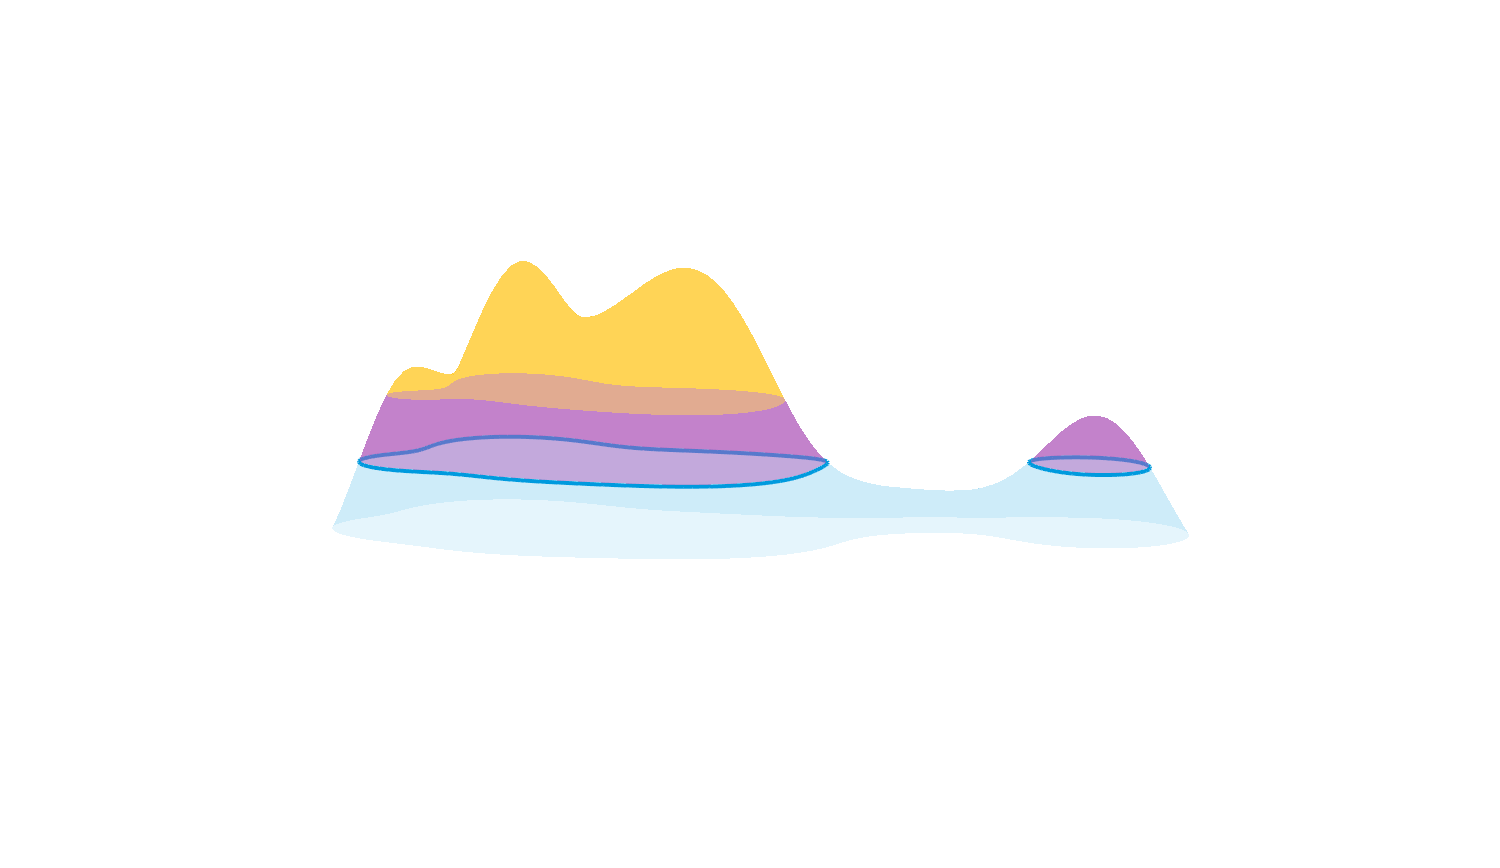
\includegraphics[trim=200 200 200 100, clip, width=\textwidth]{scripts/figures/surf/ass2_C_side.png}\\
    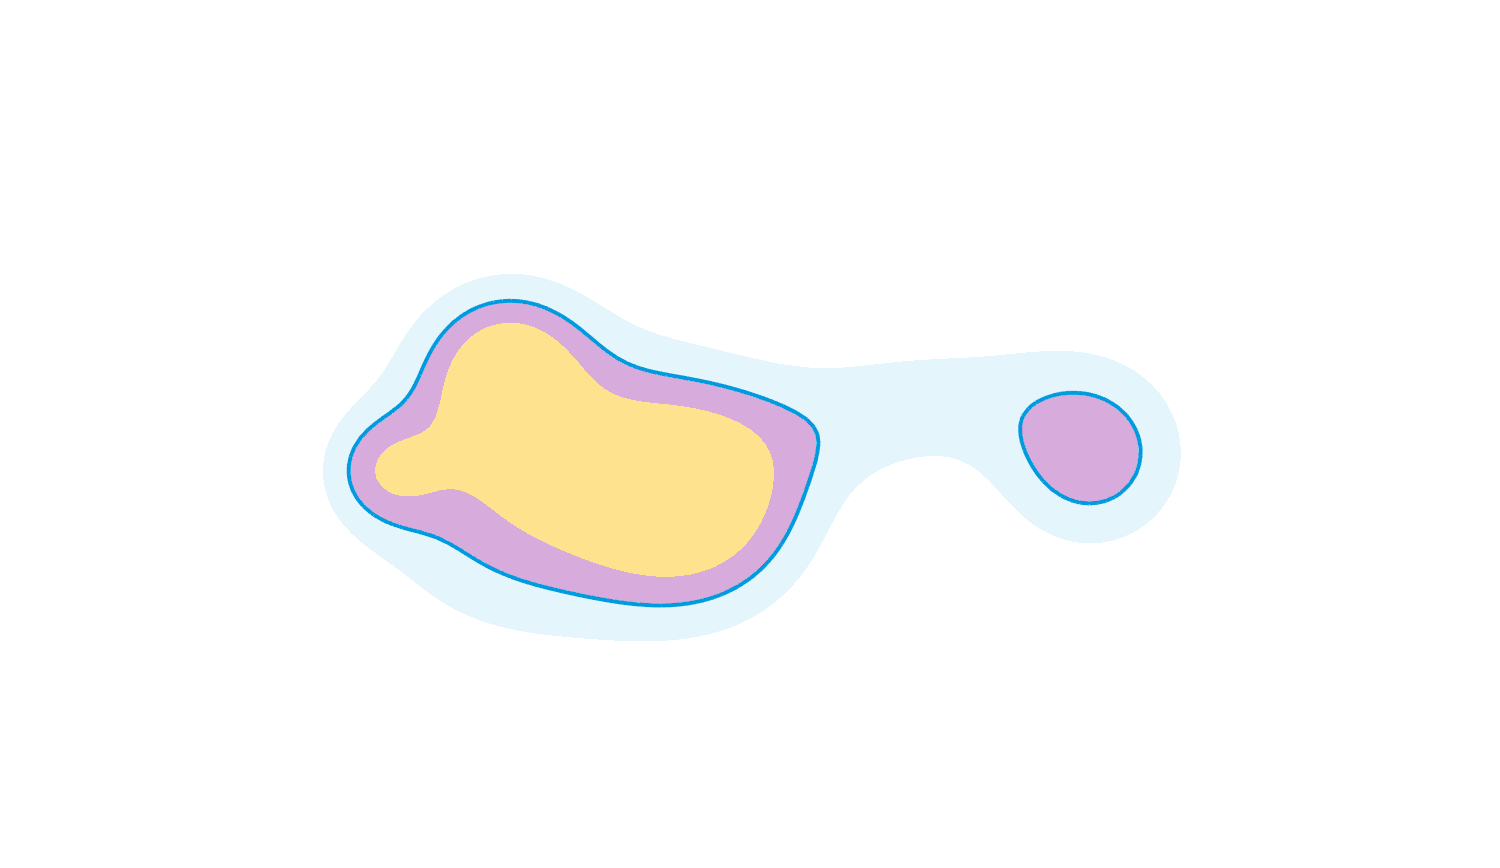
\includegraphics[trim=200 100 200 200, clip, width=\textwidth]{scripts/figures/surf/ass2_C_top.png}
  \end{minipage}
  \begin{minipage}[b]{0.7\textwidth}
    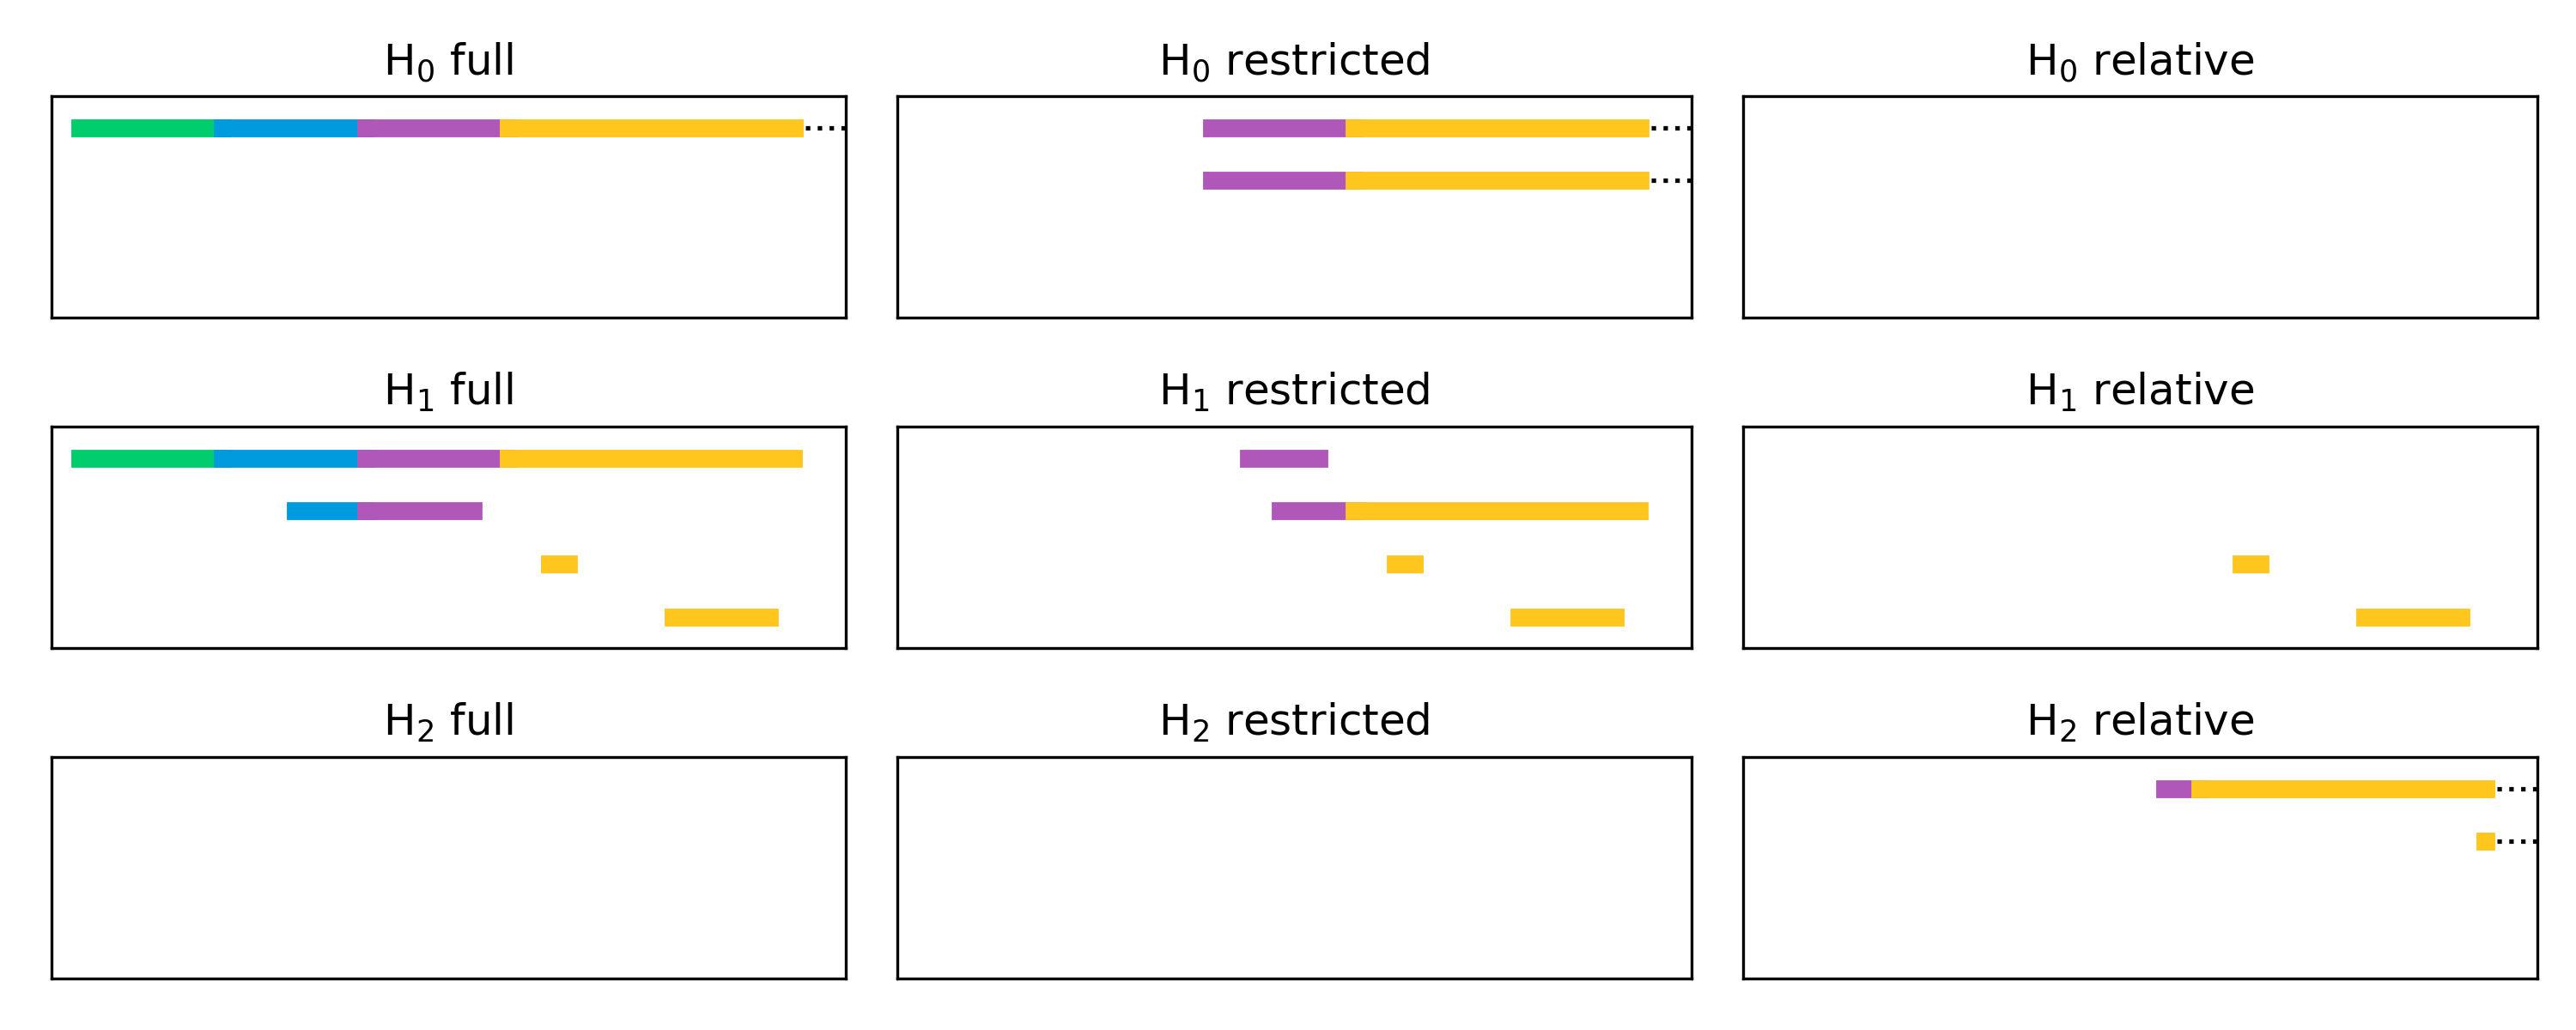
\includegraphics[width=\textwidth]{scripts/figures/barcodes/res_rel.png}
  \end{minipage}
  \caption{Full, restricted, and relative barcodes of the function (left).}
\end{figure}

Let $\LL^k$ denote the $k$th persistent homology module of the sublevel set filtration $\{B_\alpha\}_{\alpha\in\R}$.
As in the previous section, let $\DD{\omega}^k$ denote the $k$th persistent (relative) homology module of $\{(D\subi{\omega}{\alpha}, B_\omega)\}_{\alpha\in\R}$.
Throughout we will assume that we are taking homology in a field $\FF$ and that the homology groups $\hom_k(B_\alpha)$ and $\hom_k(D\subi{\omega}{\alpha}, B_\omega)$ are finite dimensional vector spaces for all $k$ and $\alpha\in\R$.
We will use the interval decomposition of $\LL^k$ to give a decomposition of the relative module $\DD{\omega}^k$ in terms of a \emph{truncation} of $\LL^k$.
For fixed $\omega\in\R$ we will define the truncation $\T^k_\omega$ of $\LL^k$ in terms of the intervals decomposing $\LL^k$ that are in $[\omega, \infty)$.

\paragraph*{Truncated Interval Modules}

For an interval $I = [s,t)\subseteq \R$ let $I_+ := [t,\infty)$ and $I_- := (-\infty, s]$.
For $\omega\in\R$ let $\FF_{\omega}^I$ denote the interval module consisting of vector spaces $\{F\subi{\omega}{\alpha}^I\}_{\alpha\in\R}$ and linear maps $\{f\subi{\omega}{\alpha,\beta}^I : F\subi{\omega}{\alpha}^I\to F\subi{\omega}{\beta}^I\}_{\alpha\leq\beta}$ where
\[ F\subi{\omega}{\alpha}^I := \begin{cases} F_\alpha^I&\text{ if } \omega\in I_-\\ 0&\text{ otherwise,}\end{cases}\ \text{ and }\ \ f\subi{\omega}{\alpha,\beta}^I := \begin{cases} f_{\alpha,\beta}^I&\text{ if } \omega\in I_-\\ 0&\text{ otherwise.}\end{cases}\]
For a collection $\I$ of intervals let $\I_\omega := \{I\in\I\mid \omega\in I\}$.

\begin{lemma}\label{lem:decomposition}
  Suppose $\I^k$ and $\I^{k-1}$ are collections of intervals that decompose $\LL^k$ and $\LL^{k-1}$, respectively.
  Then for all $k$ the $k$th persistent homology module of $\{(D\subi{\omega}{\alpha}, B_\omega)\}_{\alpha\in\R}$ is isomorphic to
  \[\bigoplus_{I\in\I^k} \FF_\omega^I \oplus \bigoplus_{I\in \I_\omega^{k-1}} \FF^{I_+}.\]
\end{lemma}
\begin{proof}
  Suppose $\alpha\leq\omega$.
  So $\hom_k(D\subi{\omega}{\alpha}, B_\omega) = 0$ as $D\subi{\omega}{\alpha} = B_\omega\cup B_\alpha$ and $\T^k_\omega = 0$ as $F_\alpha^I = 0$ for any $I\in \I^k$ such that $\omega\in I_-$.
  Moreover, $\omega\in I$ for all $I\in \I_\omega^{k-1}$, thus $F_\alpha^{I_+} = 0$ for all $\alpha\leq\omega$.
  So it suffices to assume $\omega < \alpha$.

  Consider the long exact sequence of the pair $\hom_k(D\subi{\omega}{\alpha}, B_\omega) = \hom_k(B_\alpha, B_\omega)$
  \[ \ldots\to \hom_k(B_\omega)\xrightarrow{p_\alpha^k} \hom_k(B_\alpha)\xrightarrow{q_\alpha^k}\hom_k(D\subi{\omega}{\alpha}, B_\omega)\xrightarrow{r_\alpha^k} \hom_{k-1}(B_\omega)\xrightarrow{p_\alpha^{k-1}}\hom_{k-1}(B_\alpha)\to\ldots\]
  where $\hom_k(B_\alpha) = \bigoplus_{I\in \I^k}F_\alpha^I$, $\hom_k(B_\omega) = \bigoplus_{I\in \I^k}F_\omega^I$, and $p_\alpha^k = \displaystyle\bigoplus_{I\in\I^k} f_{\omega,\alpha}^I$.

  Noting that $\im~q_\alpha^k \cong \hom_k(B_\alpha) / \ker~q_\alpha^k$ where $\ker~q_\alpha^k = \im~p_\alpha^k$ by exactness we have $\ker~r_\alpha^k \cong \hom_k(B_\alpha) / \im~p_\alpha^k$.
  By the definition of $F_\alpha^I$ and $f_{\omega,\alpha}^I$ we know $\im~f_{\omega,\alpha}^I$ is $F_\alpha^I$ if $\omega\in I$ and 0 otherwise.
  As $\im~p_\alpha^k$ is equal to the direct sum of images $\im~f_{\omega,\alpha}^I$ over $I\in\I^k$ it follows that $\im~p_\alpha^k$ is the direct sum of those $F_\alpha^I$ over those $I\in\I^k$ such that $\omega\in I$.
  Now, because $\hom_k(B_\alpha) = \bigoplus_{I\in \I^k}F_\alpha^I$ and each $F_\alpha^I$ is either 0 or $\FF$ the quotient $\hom_k(B_\alpha) / \im~p_\alpha^k$ is the direct sum of those $F_\alpha^I$ such that $\omega\notin I$.
  Therefore, by the definition of $F\subi{\omega}{\alpha}^I$ we have
  \[ \ker~r_\alpha^k = \bigoplus_{I\in\I_\omega^k} F\subi{\omega}{\alpha}^I.\]

  Similarly, $\im~r_\alpha^k = \ker~p_\alpha^{k-1}$ by exactness where $\ker~p_\alpha^{k-1}$ is the direct sum of kernels $\ker~f_{\omega,\alpha}^I$ over $I\in\I^{k-1}$.
  By the definition of $F_\alpha^I$ and $f_{\omega,\alpha}^I$ we know that $\ker~f_{\omega,\alpha}^I$ is $F_\alpha^I$ if $\omega\notin I$ and $0$ otherwise.
  Noting that $\ker~f_{\omega,\alpha}^I = 0$ for any $I\in \I^{k-1}$ such that $\omega\notin I$ it suffices to consider only those $I\in \I_\omega^{k-1}$.
  It follows that $\ker~f_{\omega,\alpha}^I = F_\alpha^{I_+}$ for any $I$ containing $\omega$ as $\omega < \alpha$.
  Therefore,
  \[\im~r_\alpha^k = \bigoplus_{I\in\I^{k-1}} F_\alpha^{I_+}.\]

  We have the following split exact sequence associated with $r_\alpha^k$
  \[ 0\to \ker~r_\alpha^k\to \hom_k(D\subi{\omega}{\alpha}, B_\omega)\to\im~r_\alpha^k\to 0.\]
  The desired result follows from the fact that for all $\alpha\in\R$
  \begin{align*}
    \hom_k(D\subi{\omega}{\alpha}, B_\omega) &\cong \ker~r_\alpha^k\oplus \im~r_\alpha^k =\bigoplus_{I\in\I^k} F\subi{\omega}{\alpha}^I\oplus \bigoplus_{I\in\I_\omega^{k-1}} F_\alpha^{I_+}.
  \end{align*}
\end{proof}

Letting $\I^k$ denote the decomposing intervals of $\LL^k$ for all $k$ we can define the \textbf{$\omega$-truncated $k$th persistent homology module} of $\LL^k$ as
\[ \T_\omega^k := \bigoplus_{I\in\I^k} \FF_\omega^I\ \text{ and let }\ \LL_\omega^{k-1} := \bigoplus_{I\in \I_\omega^{k-1}} \FF^{I_+}\]
denote the submodule of $\DD{\omega}^k$ consisting of intervals $[\beta,\infty)$ corresponding to features $[\alpha,\beta)$ in $\LL^{k-1}$ such that $\alpha\leq\omega <\beta$.
Now, by Lemma~\ref{lem:decomposition} the $k$th persistent (relative) homology module of $\{(D\subi{\omega}{\alpha}, B_\omega)\}_{\alpha\in\R}$ is $\DD{\omega}^k = \T_\omega^k\oplus \LL_\omega^{k-1}.$
Theorems~\ref{thm:algo_tcc} and~\ref{thm:interleaving_main_2} can then be used to show that
\[ \{\rips^{2\delta}(P\subi{\omega-2c\delta}{\alpha}, Q_{\omega-2c\delta})\hookrightarrow \rips^{4\delta}(P\subi{\omega+c\delta}{\alpha}, Q_{\omega+c\delta})\}_{\alpha\in\R} \]
is $4c\delta$ interleaved with $\T_\omega^k\oplus \LL_\omega^{k-1}$ whenever
\[ \rk~\hom_d(\rips^\delta(P, Q_{\omega - 2c\delta})\hookrightarrow \rips^{2\delta}(P, Q_{\omega+c\delta})) \geq \dim~\hom_0(\rips^\delta(P\setminus Q_{\omega-2c\delta})).\]


%   If $\rk~\hom_d(\rips^\delta(P, Q_{\omega - 2c\delta})\hookrightarrow \rips^{2\delta}(P, Q_{\omega+c\delta})) \geq \dim~\hom_0(\rips^\delta(P\setminus Q_{\omega-2c\delta}))$ then the $k$th (relative) homology module of $\{\rips^{2\delta}(P\subi{\omega-2c\delta}{\alpha}, Q_{\omega-2c\delta})\hookrightarrow \rips^{4\delta}(P\subi{\omega+c\delta}{\alpha}, Q_{\omega+c\delta})\}_{\alpha\in\R}$ is $4c\delta$-interleaved with $\T_{\omega}^k \oplus \LL_\omega^{k-1}$: the $k$th persistent homology module of $\{(D\subi{\omega}{\alpha}, B_\omega)\}_{\alpha\in\R}$.
%
% Our main theorem combines this decomposition with our coverage and interleaving results of Theorems~\ref{thm:algo_tcc} and~\ref{thm:interleaving_main_2}.% as a method for certified approximation of the truncated persistence diagram.\textbf{TODO: GROSS}

% \begin{lemma}\label{lem:dual_ass}
%   Let $\X$ be an orientable $d$-manifold and suppose $(D, B)$ and $(D, B')$ are compact, locally contractible, surrounding pairs in $\X$ such that $\hom_d(D, B)$ and $\hom_d(D, B')$ are finitely generated.
%
%   If $\hom_{d-1}(B\hookrightarrow B')$ is surjective then $\hom_0(D\setminus B'\hookrightarrow D\setminus B)$ is injective.
%   If $\hom_{d-1}(B\hookrightarrow B')$ is injective then $\hom_0(D\setminus B'\hookrightarrow D\setminus B)$ is surjective.
% \end{lemma}
% \begin{proof}
%   If $\hom_{d-1}(B\hookrightarrow B')$ is surjective for all $k$ then $\hom_d((D, B)\hookrightarrow (D, B'))$ is surjective by the five lemma.
%   Taking homology with coefficients in a field $\FF$ we can dualize to obtain an \emph{injective} map $\Hom(\hom_d(D,B'), \FF)\to \Hom(\hom_d(D, B), \FF)$.
%   Therefore, because we are taking coefficients in a field, we have an injective map $\hom^d(D,B')\to \hom^d(D, B)$ by the Universal Coefficient Theorem.
%
%   Because $(D, B)$ and $(D,B')$ are compact and locally connected we can apply Alexander Duality to obtain an injective map $\hom_0(\X\setminus B', \X\setminus D)\to\hom_0(\X\setminus B, \X\setminus D)$.
%   Because $B,B'$ surround $D$ in $\X$ it follows that $\hom_0(D\setminus B'\hookrightarrow D\setminus B)$ is injective.
%   It can be shown $\hom_{d-1}(B\hookrightarrow B')$ injective implies $\hom_0(D\setminus B'\hookrightarrow D\setminus B)$ surjective by a similar argument.
% \end{proof}
%
% \begin{theorem}\label{thm:main}
%   Let $\X$ be an orientable $d$-manifold and let $D$ be a compact subset of $\X$.
%   Let $f : D\to\R$ be a $c$-Lipschitz function and $\omega\in\R$, $\delta < \varrho_D/4$ be constants such that $P\subset D$ is a $(\delta, 2\delta,\omega)$-sublevel sample of $f$ and $B_{\omega-3c\delta}$ surrounds $D$ in $\X$.
%   % Let $P$ be a finite subset of $D$ such that $(P, Q_{\omega-2c\delta})$ and $(P, Q_{\omega+c\delta})$ are $\delta$-good samples of $(D, B_\omega)$.
%   % Let $P\subset \intr_\X(D)$ and suppose $D\setminus P^\delta$, $D\setminus Q_{\omega-2c\delta}^\delta$, and $D\setminus Q_{\omega+c\delta}^\delta$ are locally path connected.
%
%   Suppose $\hom_k(B_{\omega-3c\delta}\hookrightarrow B_\omega)$ is surjective and $\hom_k(B_\omega\hookrightarrow B_{\omega+5c\delta})$ is an isomorphism for all $k$.
%   If $\rk~\hom_d(\rips^\delta(P, Q_{\omega - 2c\delta})\hookrightarrow \rips^{2\delta}(P, Q_{\omega+c\delta})) \geq \dim~\hom_0(\rips^\delta(P\setminus Q_{\omega-2c\delta}))$ then the $k$th (relative) homology module of $\{\rips^{2\delta}(P\subi{\omega-2c\delta}{\alpha}, Q_{\omega-2c\delta})\hookrightarrow \rips^{4\delta}(P\subi{\omega+c\delta}{\alpha}, Q_{\omega+c\delta})\}_{\alpha\in\R}$ is $4c\delta$-interleaved with $\T_{\omega}^k \oplus \LL_\omega^{k-1}$: the $k$th persistent homology module of $\{(D\subi{\omega}{\alpha}, B_\omega)\}_{\alpha\in\R}$.
%    % that of $\{(D\subi{\omega}{\alpha}, B_\omega)\}_{\alpha\in\R}$.
% \end{theorem}
% \begin{proof}
%   If $\hom_k(B_{\omega-3c\delta}\hookrightarrow B_\omega)$ is surjective for all $k$ then, in particular, $\hom_{d-1}(B_{\omega-3c\delta}\hookrightarrow B_\omega)$ is surjective.
%   If $\hom_k(B_{\omega-3c\delta}\hookrightarrow B_\omega)$ is surjective for all $k$ then, in particular, $\hom_{d-1}(B_{\omega-3c\delta}\hookrightarrow B_\omega)$ is surjective.
%   Because $B_{\omega-3c\delta}, B_\omega$ are closed in $D$, and $D$ is compact, $(D, B_{\omega-3c\delta})$ and $(D,B_\omega)$ are compact pairs.
%   If our pairs are locally contractible then $\hom_0(D\setminus B_\omega\hookrightarrow D\setminus B_{\omega-3c\delta})$ is injective and $\hom_0(D\setminus B_{\omega-5c\delta}\hookrightarrow D\setminus B_\omega)$ is surjective by Lemma~\ref{lem:dual_ass}.
%
%   Because $\rk~\hom_d(\rips^\delta(P, Q_{\omega - 2c\delta})\hookrightarrow \rips^{2\delta}(P, Q_{\omega+c\delta})) \geq \dim~\hom_0(\rips^\delta(P\setminus Q_{\omega-2c\delta}))$ and $P\subset D$ is a $(\delta, 2\delta,\omega)$-sublevel sample of $f$ we have $D\setminus B_\omega\subseteq P^\delta$ and $Q_{\omega-2c\delta}^\delta$ surrounds $P^\delta$ in $D$ by Theorem~\ref{thm:algo_tcc}.
%   So the persistent homology modules of $\{\rips^{2\delta}(P\subi{\omega-2c\delta}{\alpha}, Q_{\omega-2c\delta})\hookrightarrow \rips^{4\delta}(P\subi{\omega+c\delta}{\alpha}, Q_{\omega+c\delta})\}_{\alpha\in\R}$ are $4c\delta$ interleaved with those of $\{(D\subi{\omega}{\alpha}, B_\omega)\}_{\alpha\in\R}$ by Theorem~\ref{thm:interleaving_main_2}, and therefore $\T_{\omega}^k \oplus \LL_\omega^{k-1}$ by Lemma~\ref{lem:decomposition}.
% \end{proof}


  \subsection{Experiments}
    % !TeX root = ../../main.tex

\begin{figure}[htbp]\label{fig:ripple1}
  \centering
  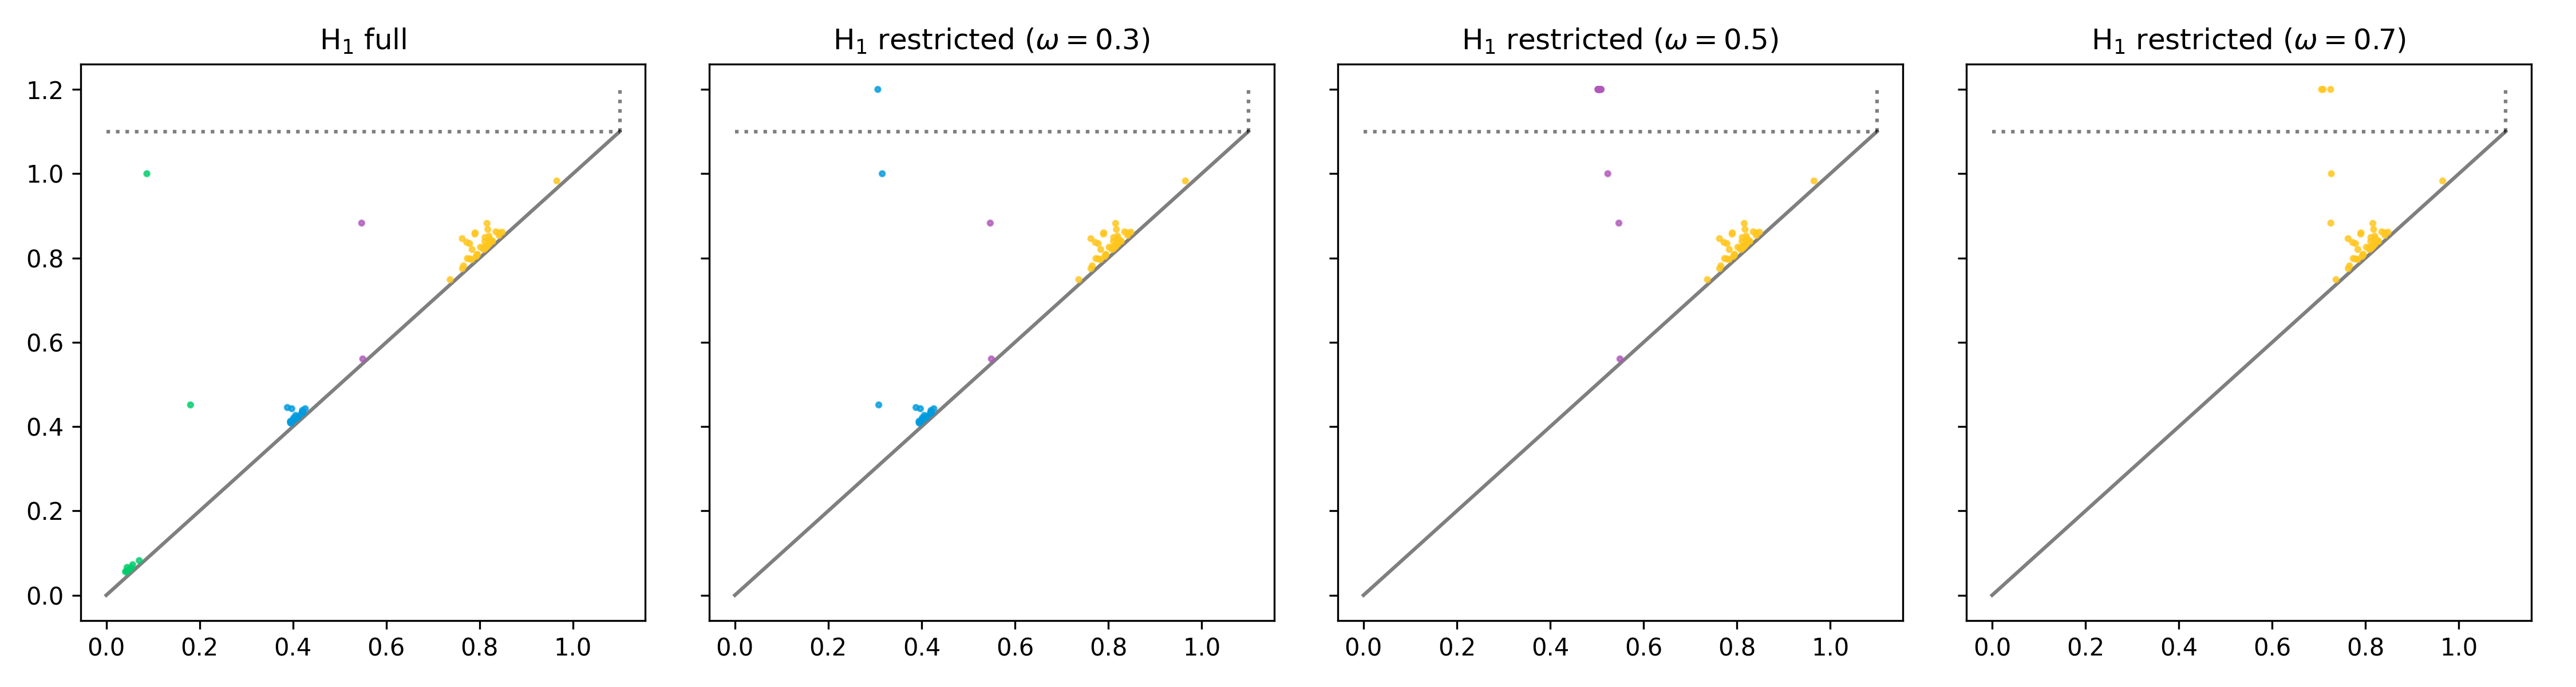
\includegraphics[trim=0 0 790 0, clip, width=0.3\textwidth]{scripts/figures/matching2/full-dgm.png}
  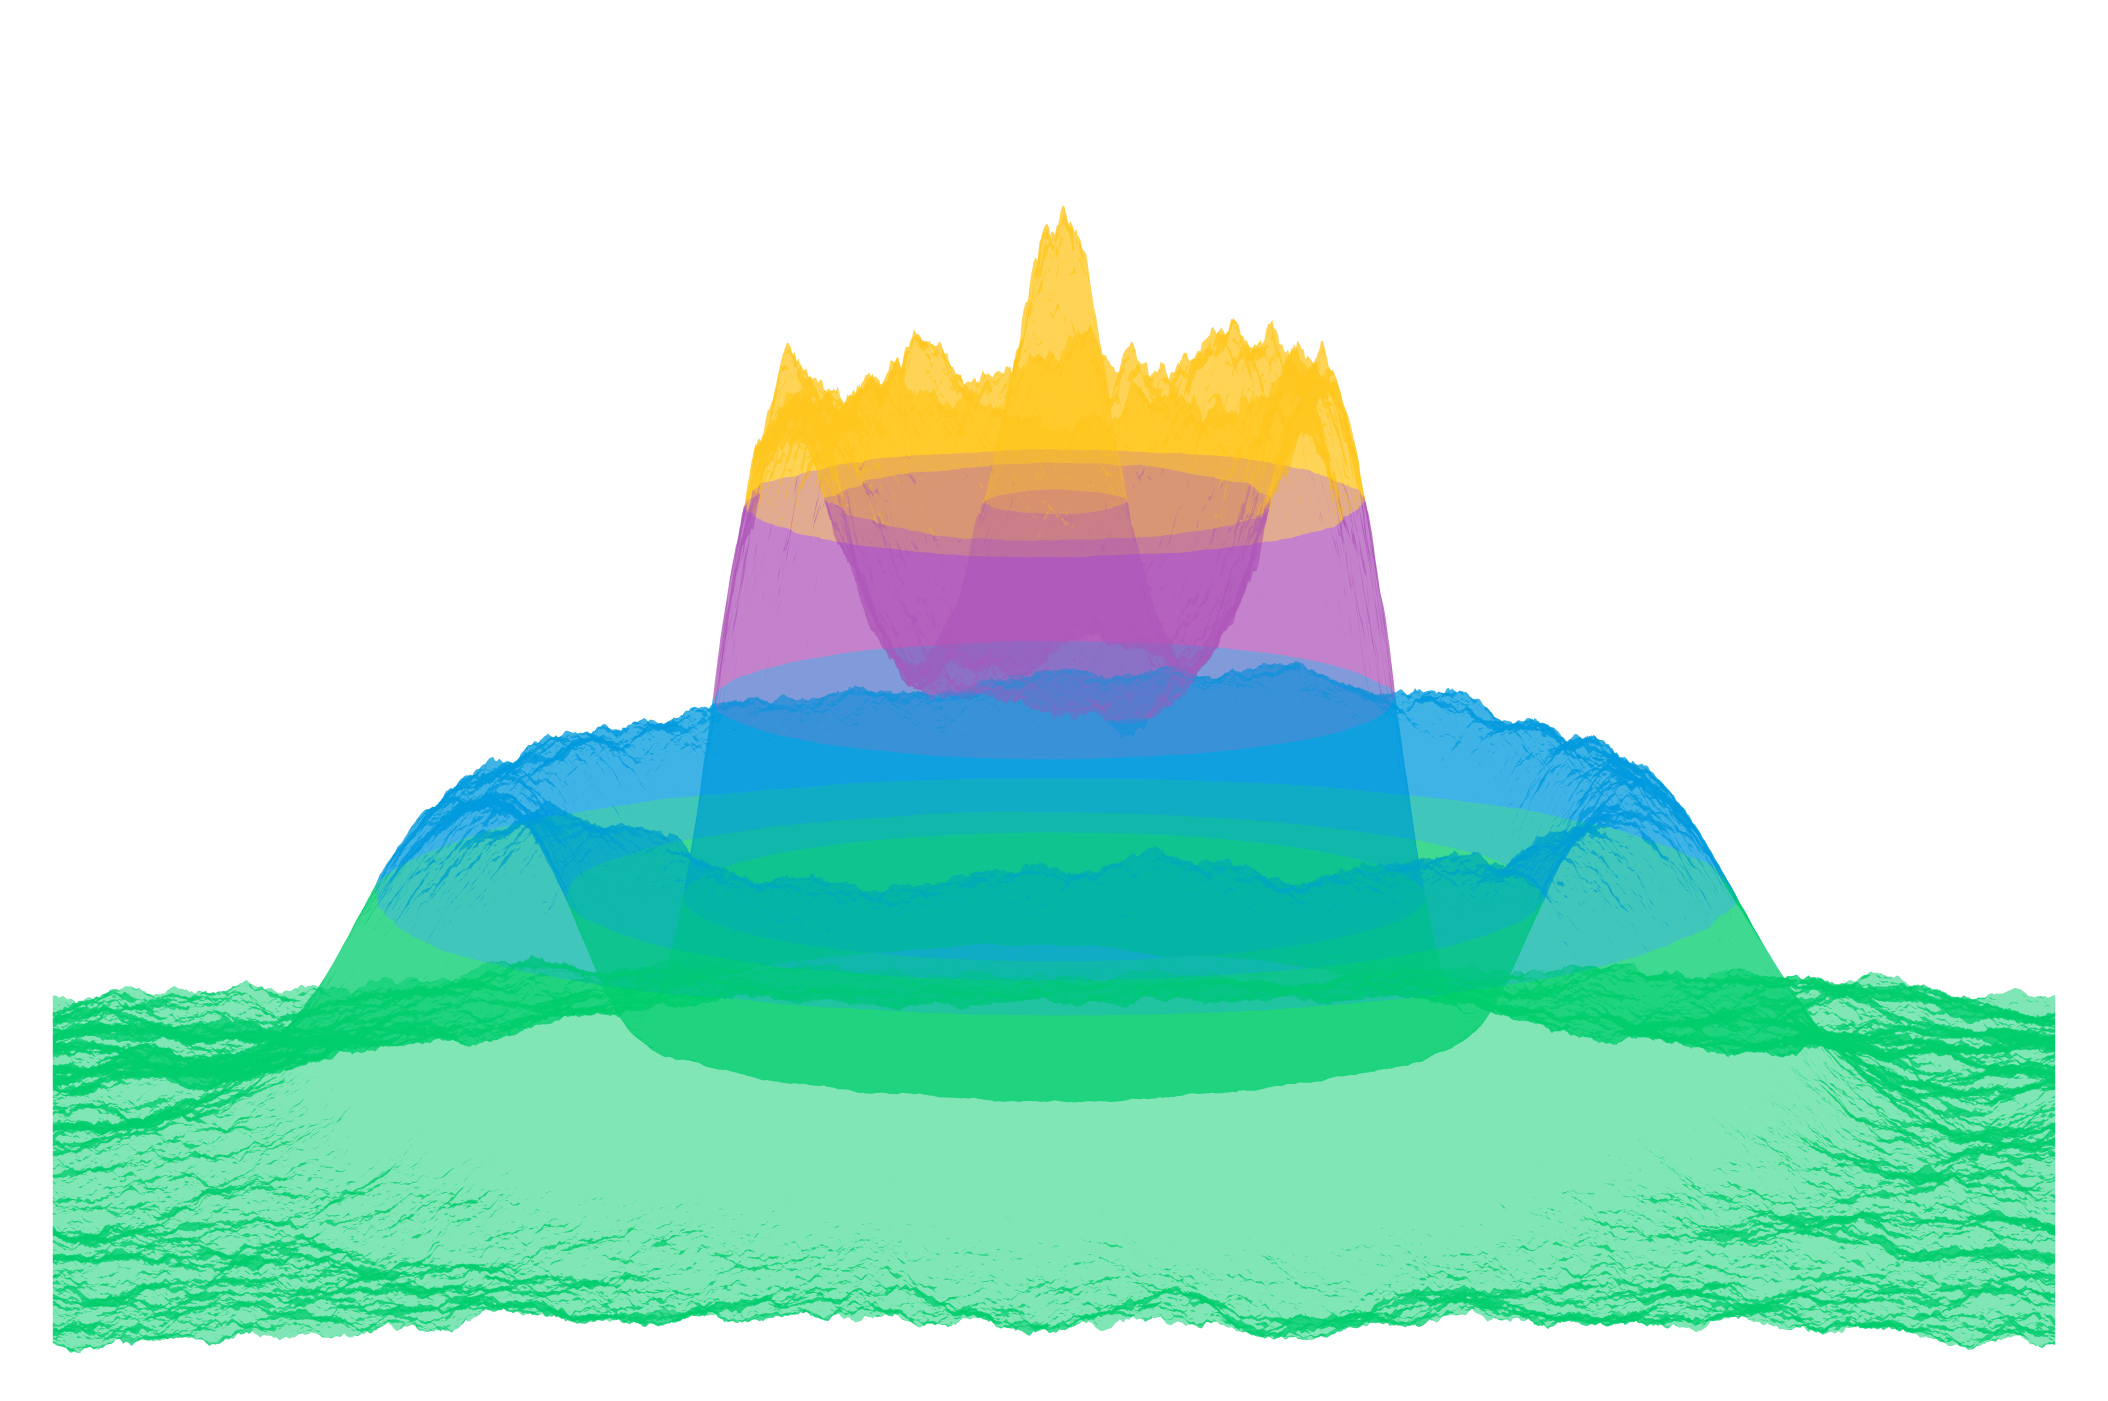
\includegraphics[trim=-350 -800 -700 -300, clip, width=0.4\textwidth]{scripts/figures/matching2/full-surf_side-lowres.png}
  
\includegraphics[trim=0 -800 0 0, width=0.25\textwidth]{scripts/figures/matching2/full-surf_top-lowres.png}
  % \includegraphics[trim=0 0 0 -10, clip, width=\textwidth]{scripts/figures/matching1/817_1024-3_1-1_1.png}
  \caption{The $\hom_1$ persistence diagram of the sinusoidal function pictured to the right.
          Features are colored by birth time, infinite features are drawn above the dotted line.}
\end{figure}

\begin{figure}[htbp]
  \centering
  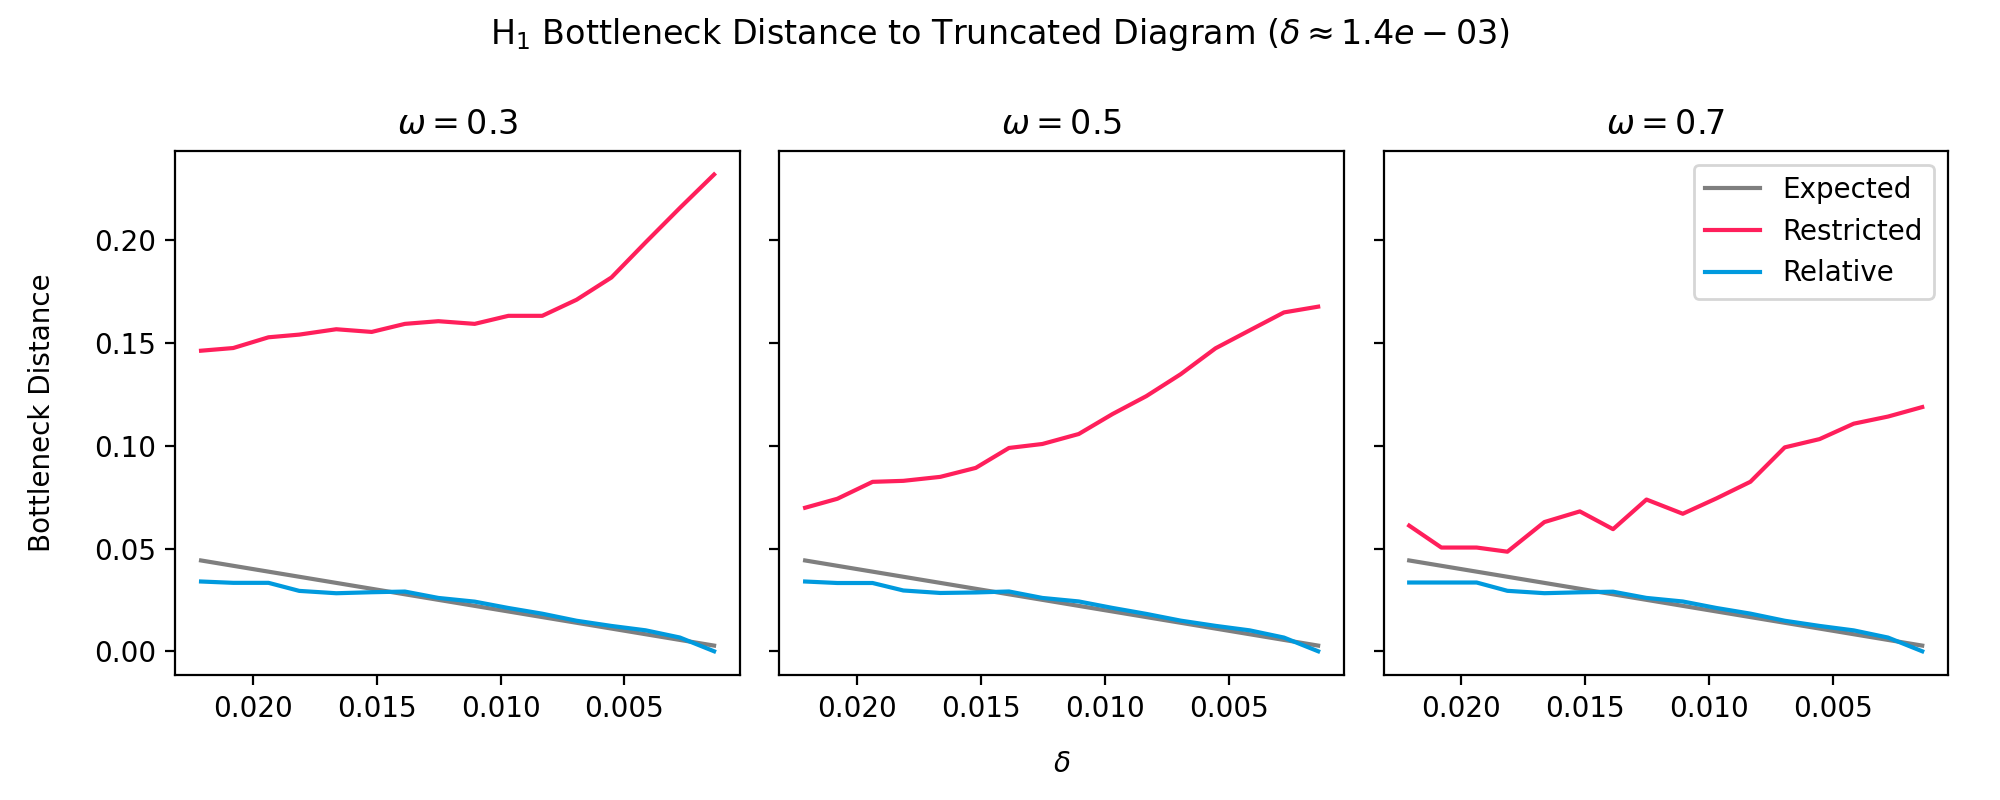
\includegraphics[width=\textwidth]{scripts/figures/matching2/bottleneck_delta.png}
  \caption{Comparison of the bottleneck distance between the truncated diagram of the function shown in Figure~\ref{fig:ripple1} approximated with $\delta\approx 1.4\times10^{-3}$ ($1024\times 1024$ grid) and those of the restricted and relative diagrams with decreasing $\delta$ (increasing grid size 64-1024).}
\end{figure}

\begin{figure}[htbp]
  \centering
  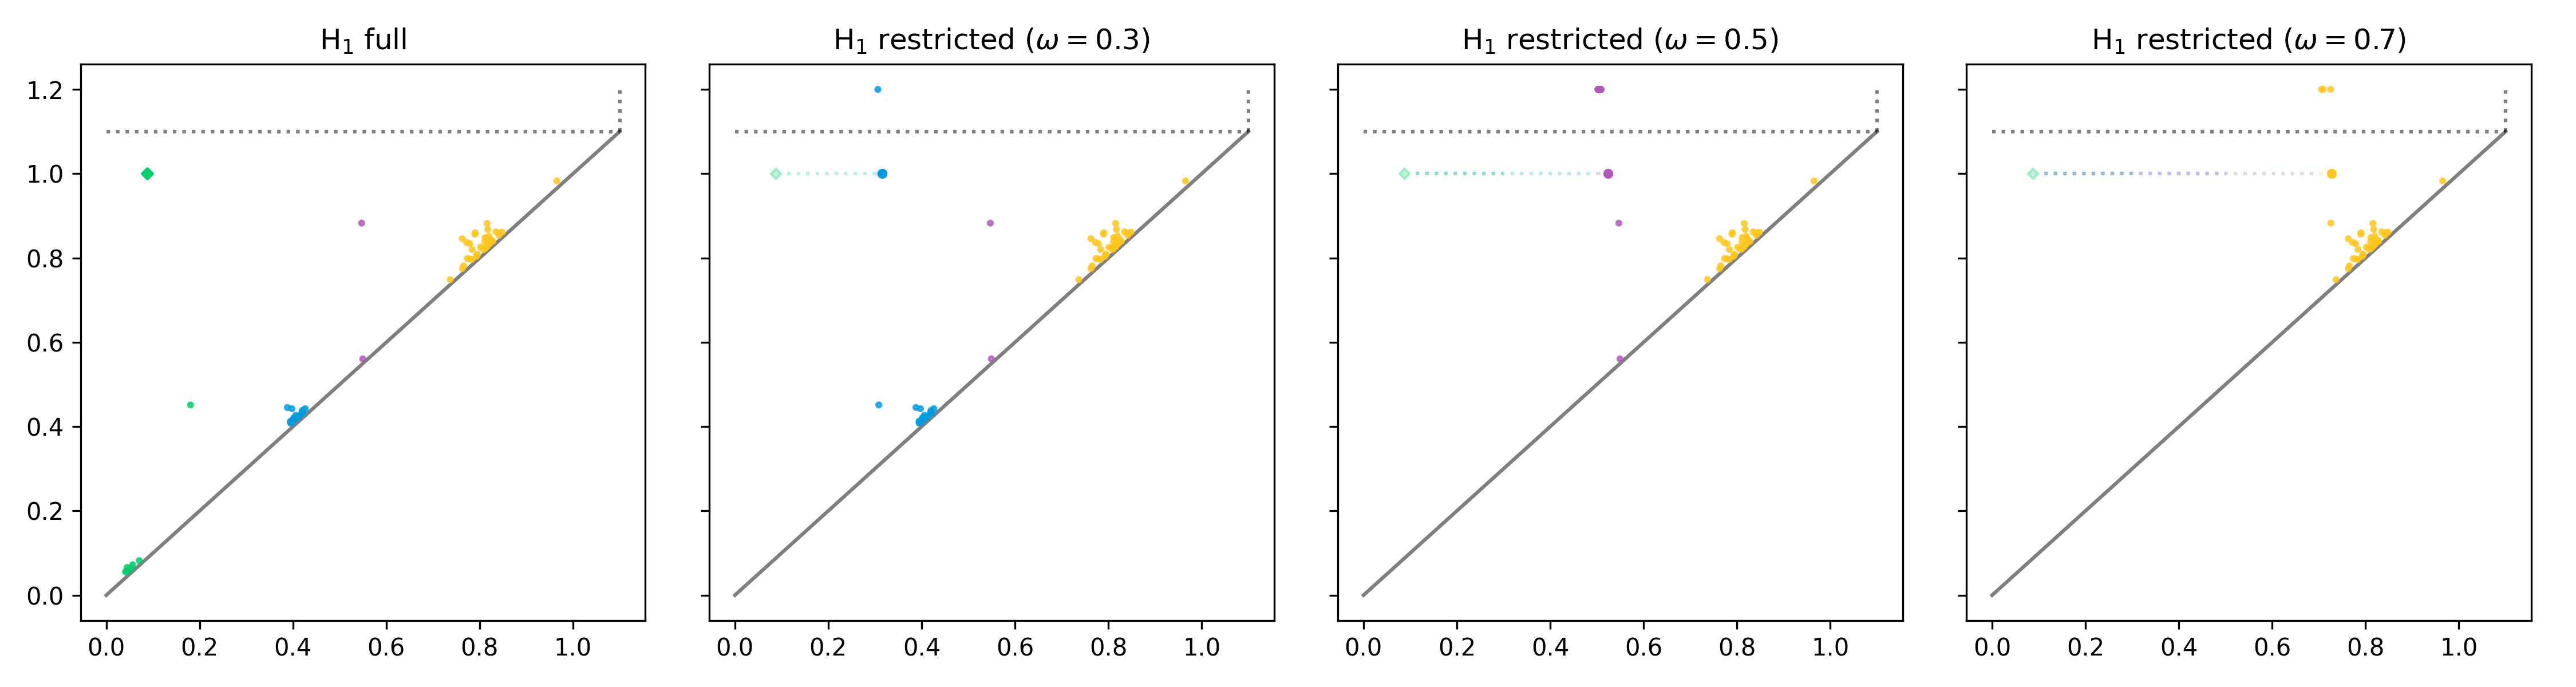
\includegraphics[trim=0 0 -10 0, clip, width=\textwidth]{scripts/figures/matching2/dgm-1.png}
  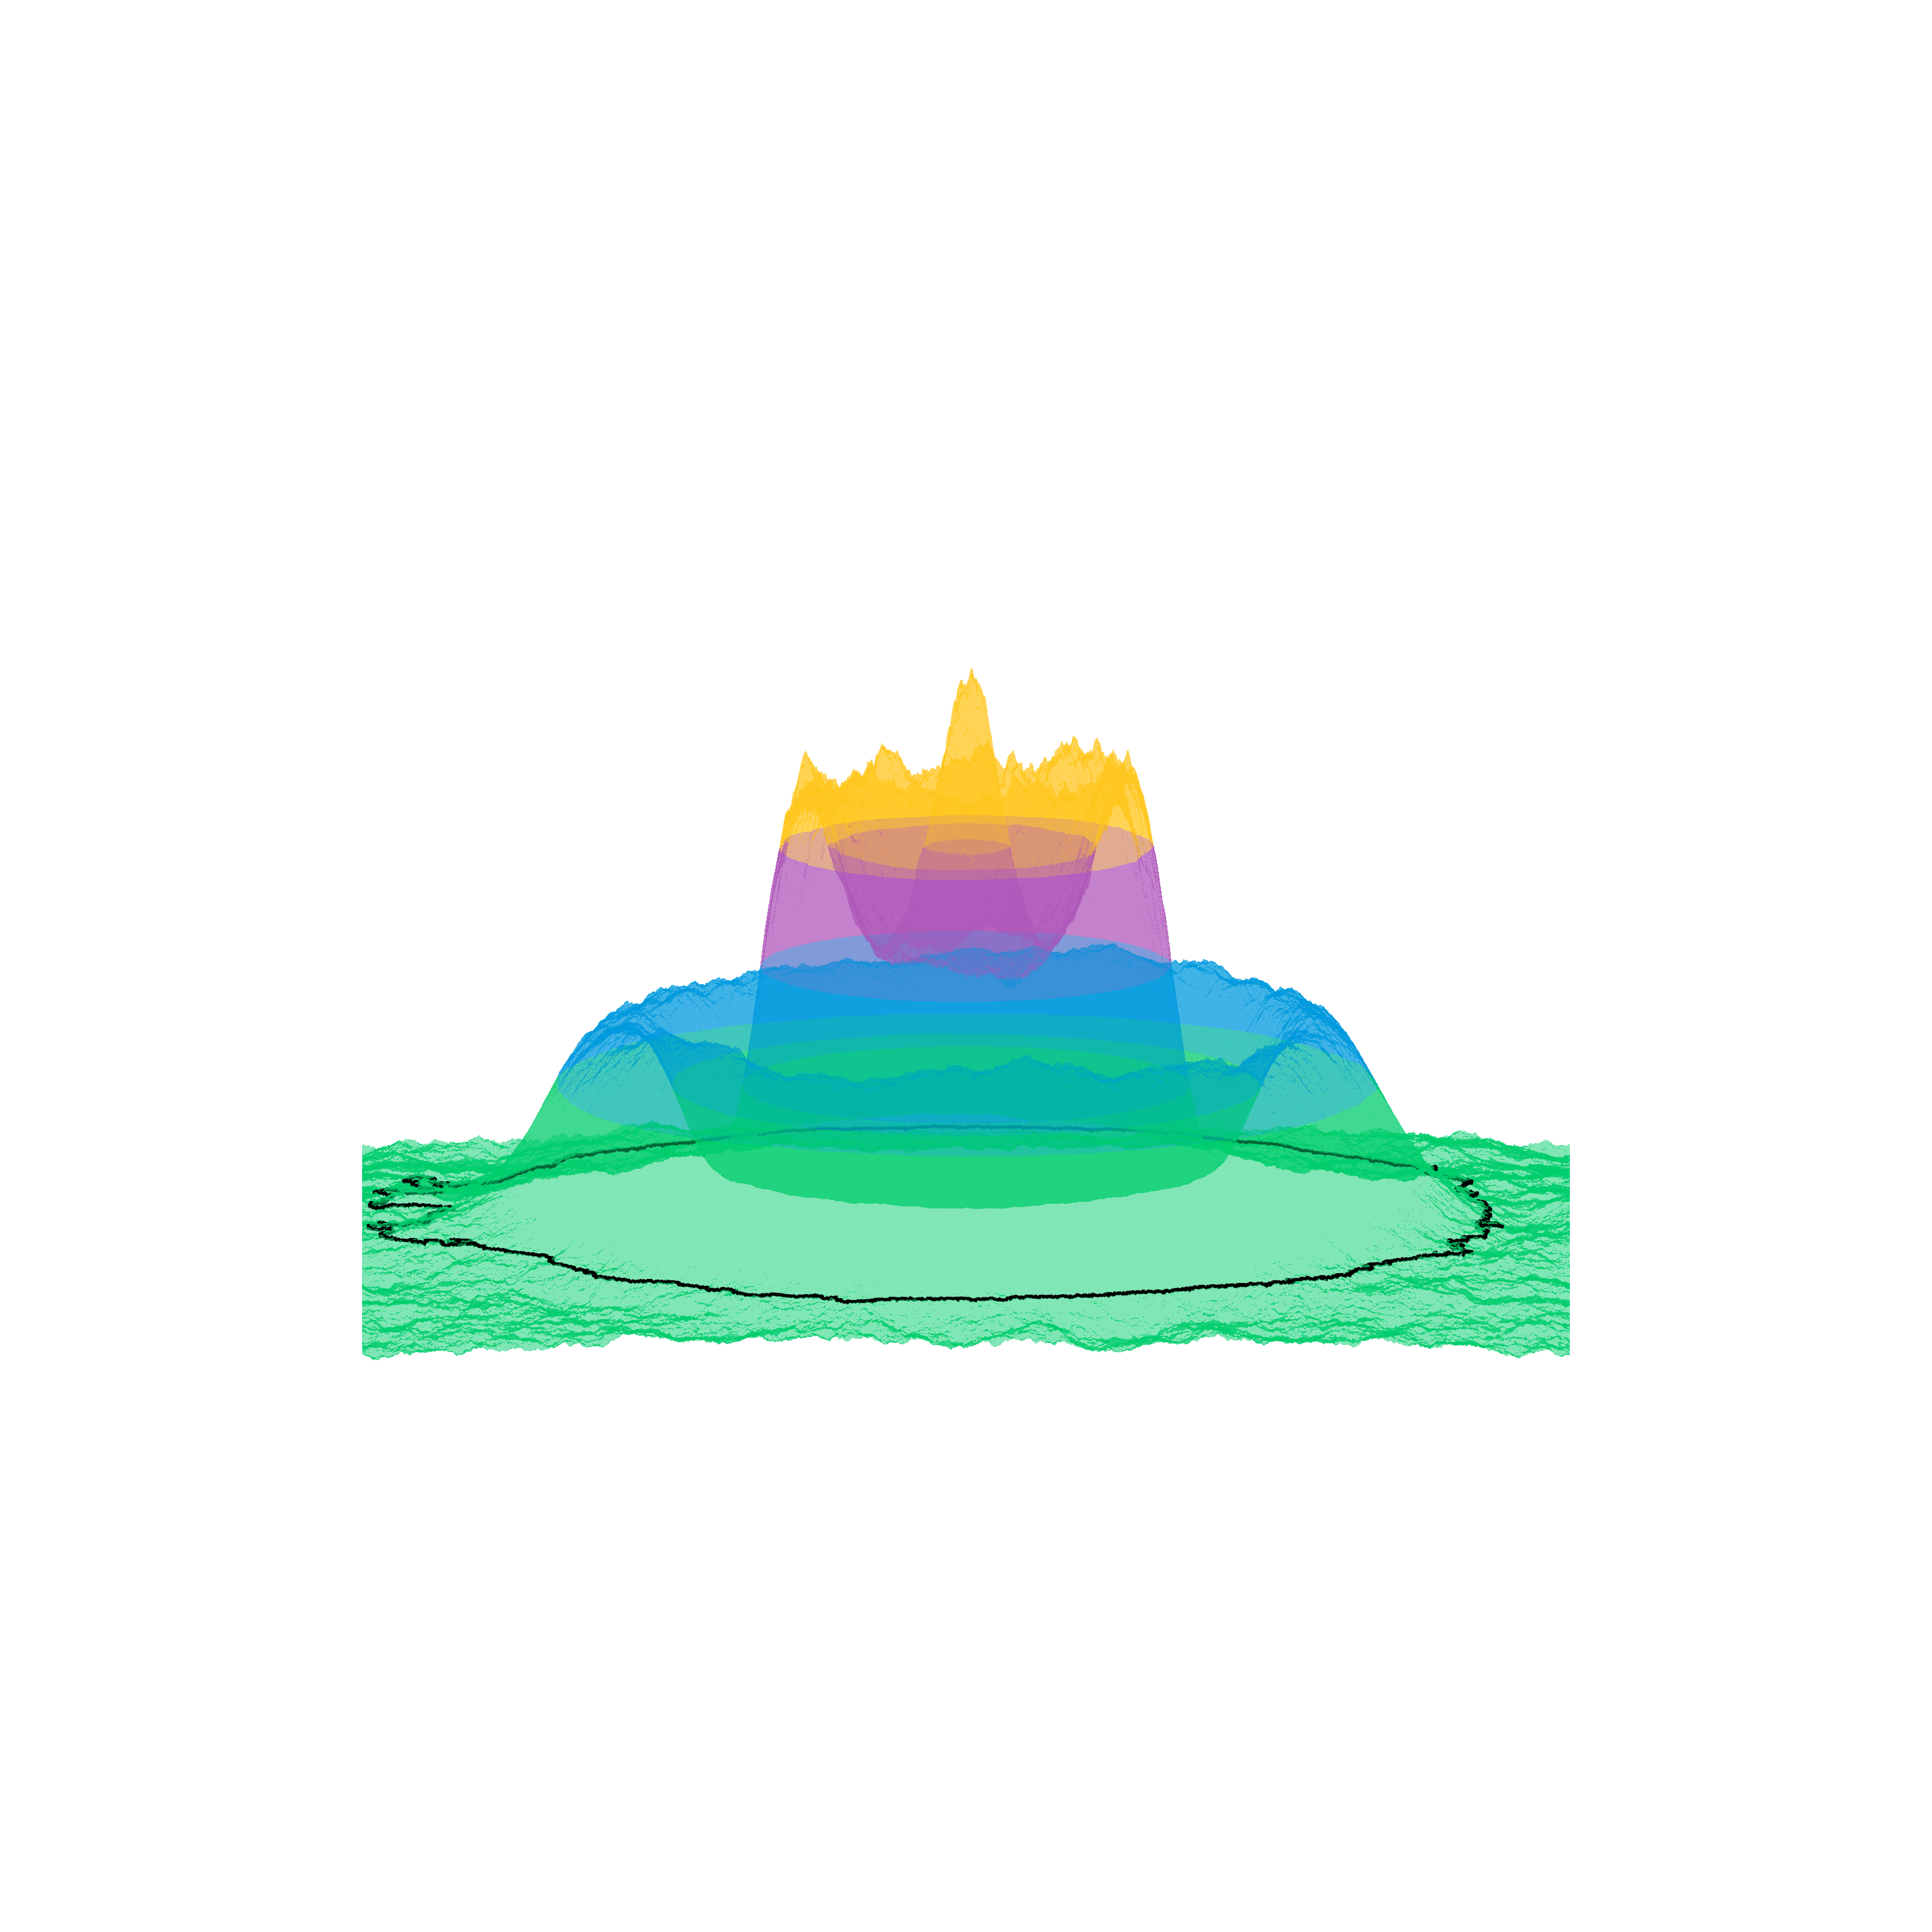
\includegraphics[trim=500 800 500 800, clip, width=0.24\textwidth]{scripts/figures/matching2/surf_side-1.png}
  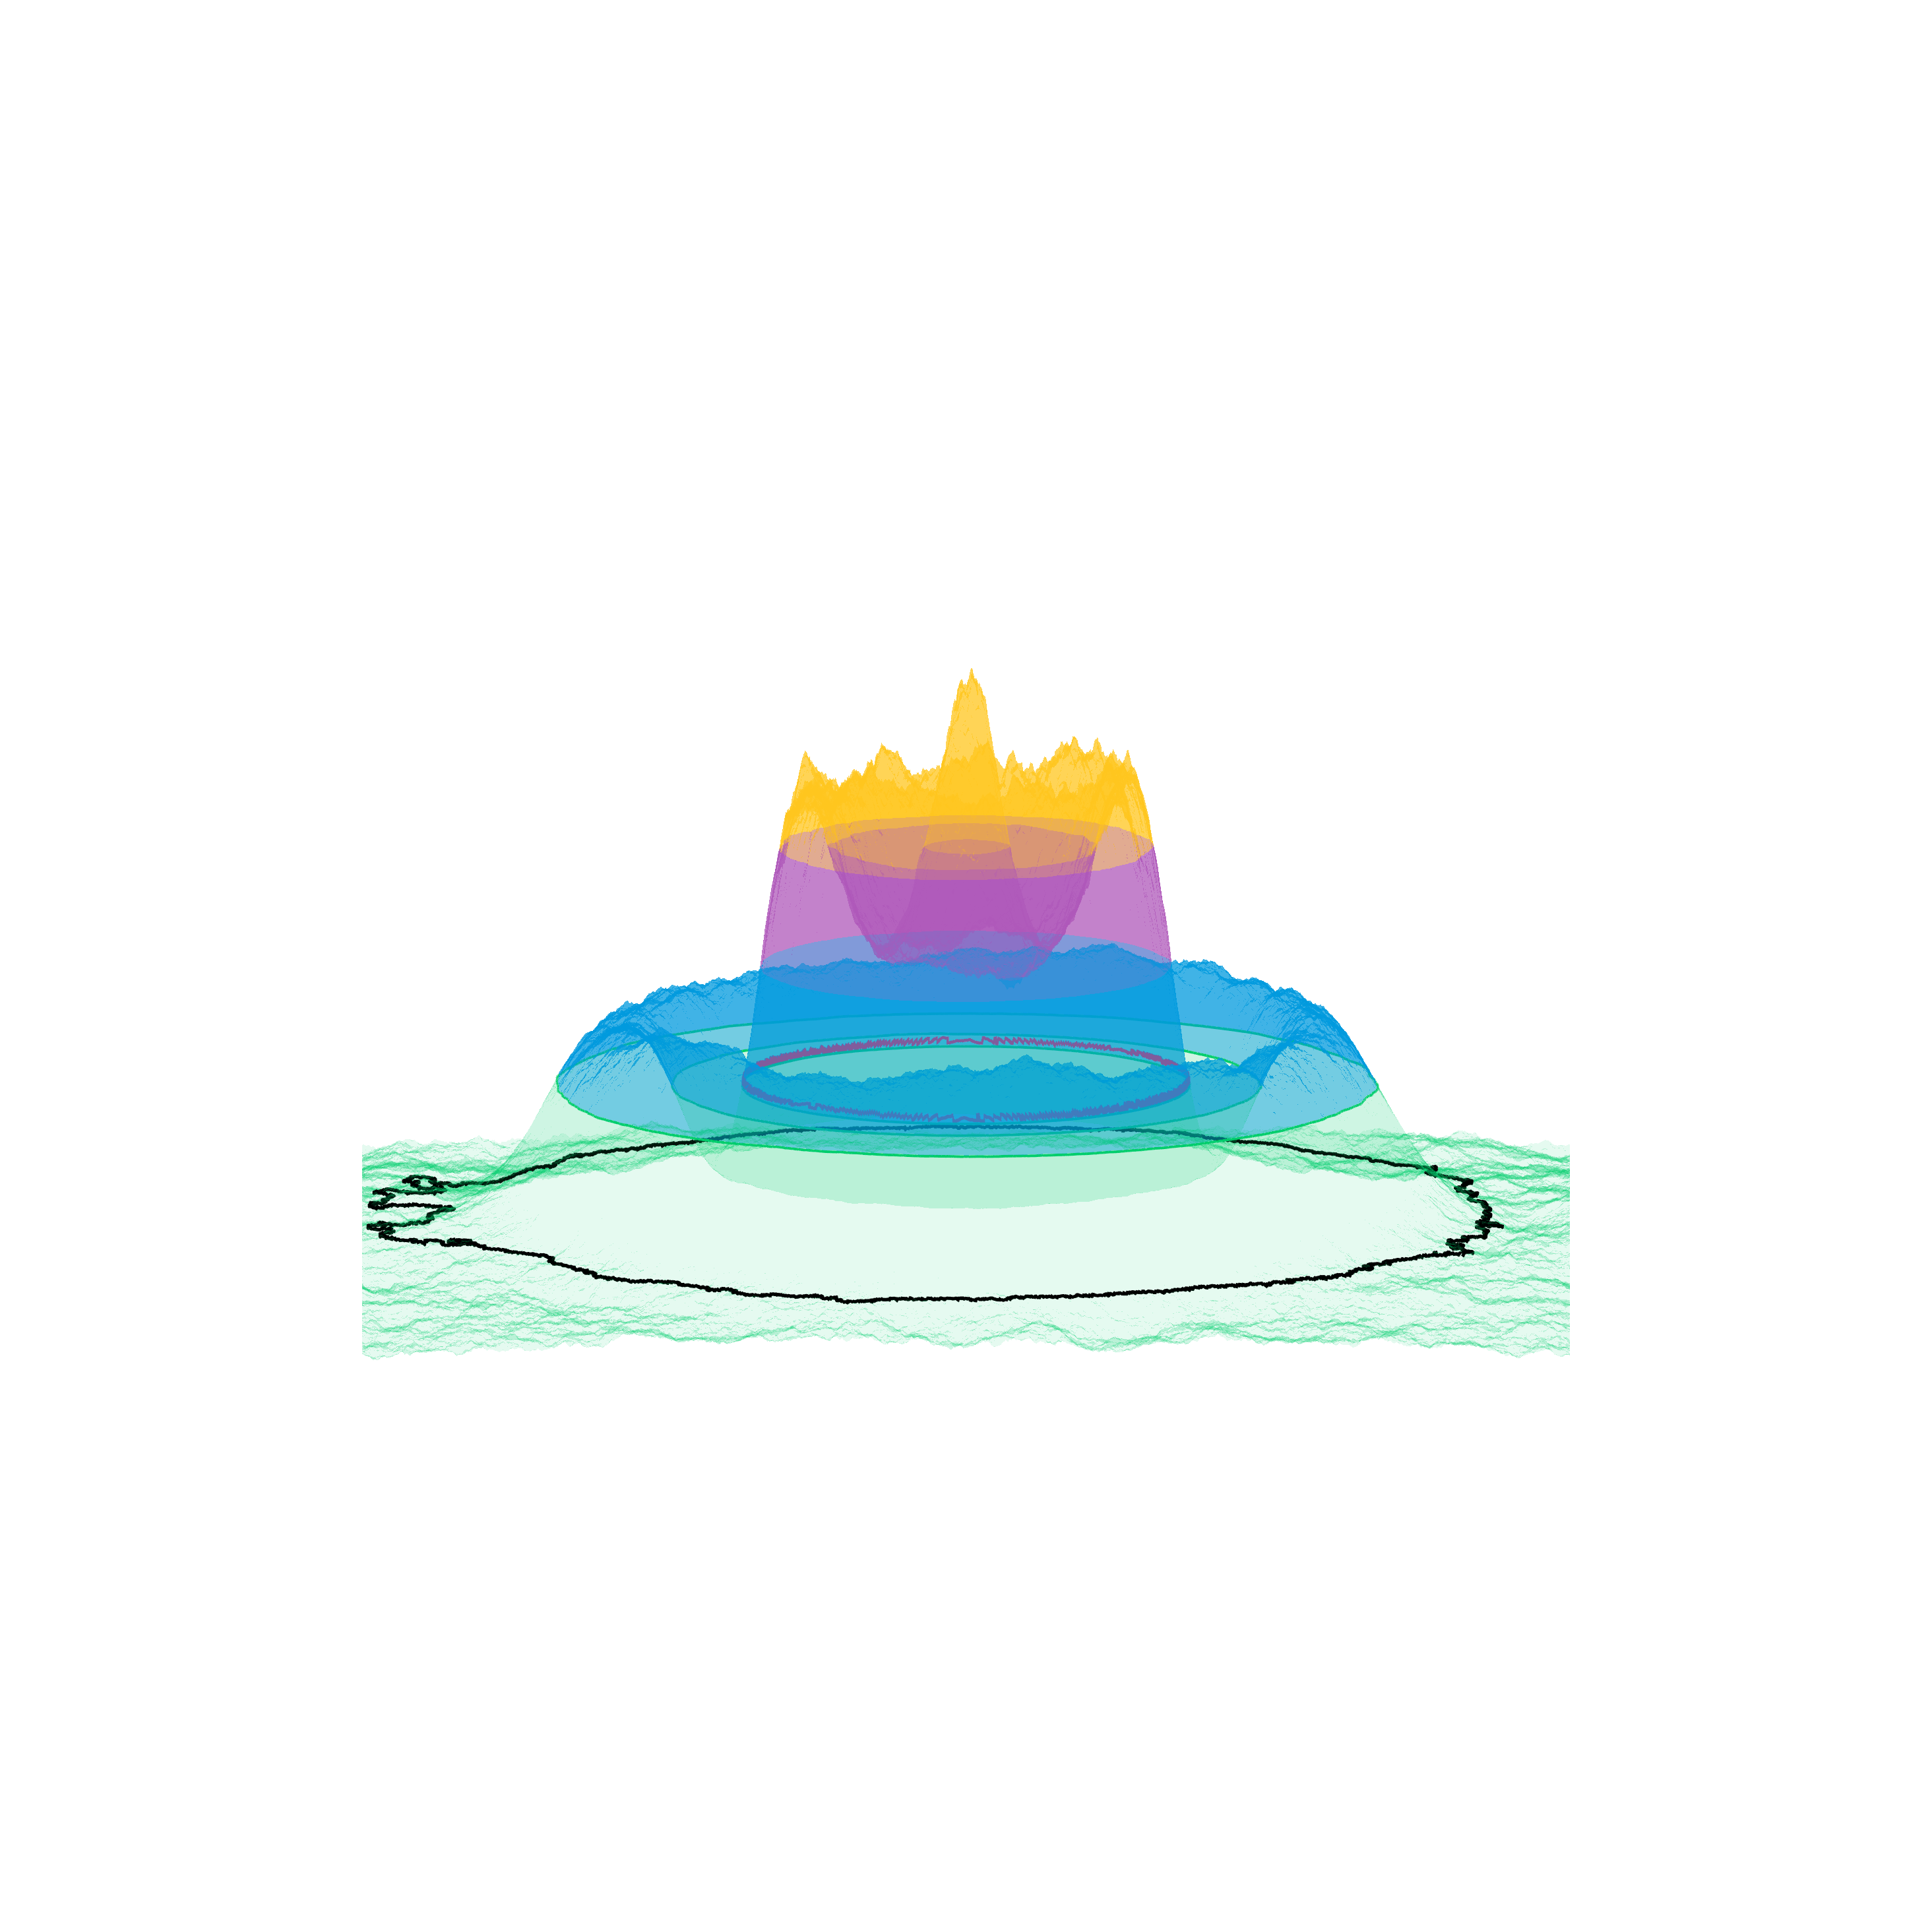
\includegraphics[trim=500 800 500 800, clip, width=0.24\textwidth]{scripts/figures/matching2/surf_side-1_0.png}
  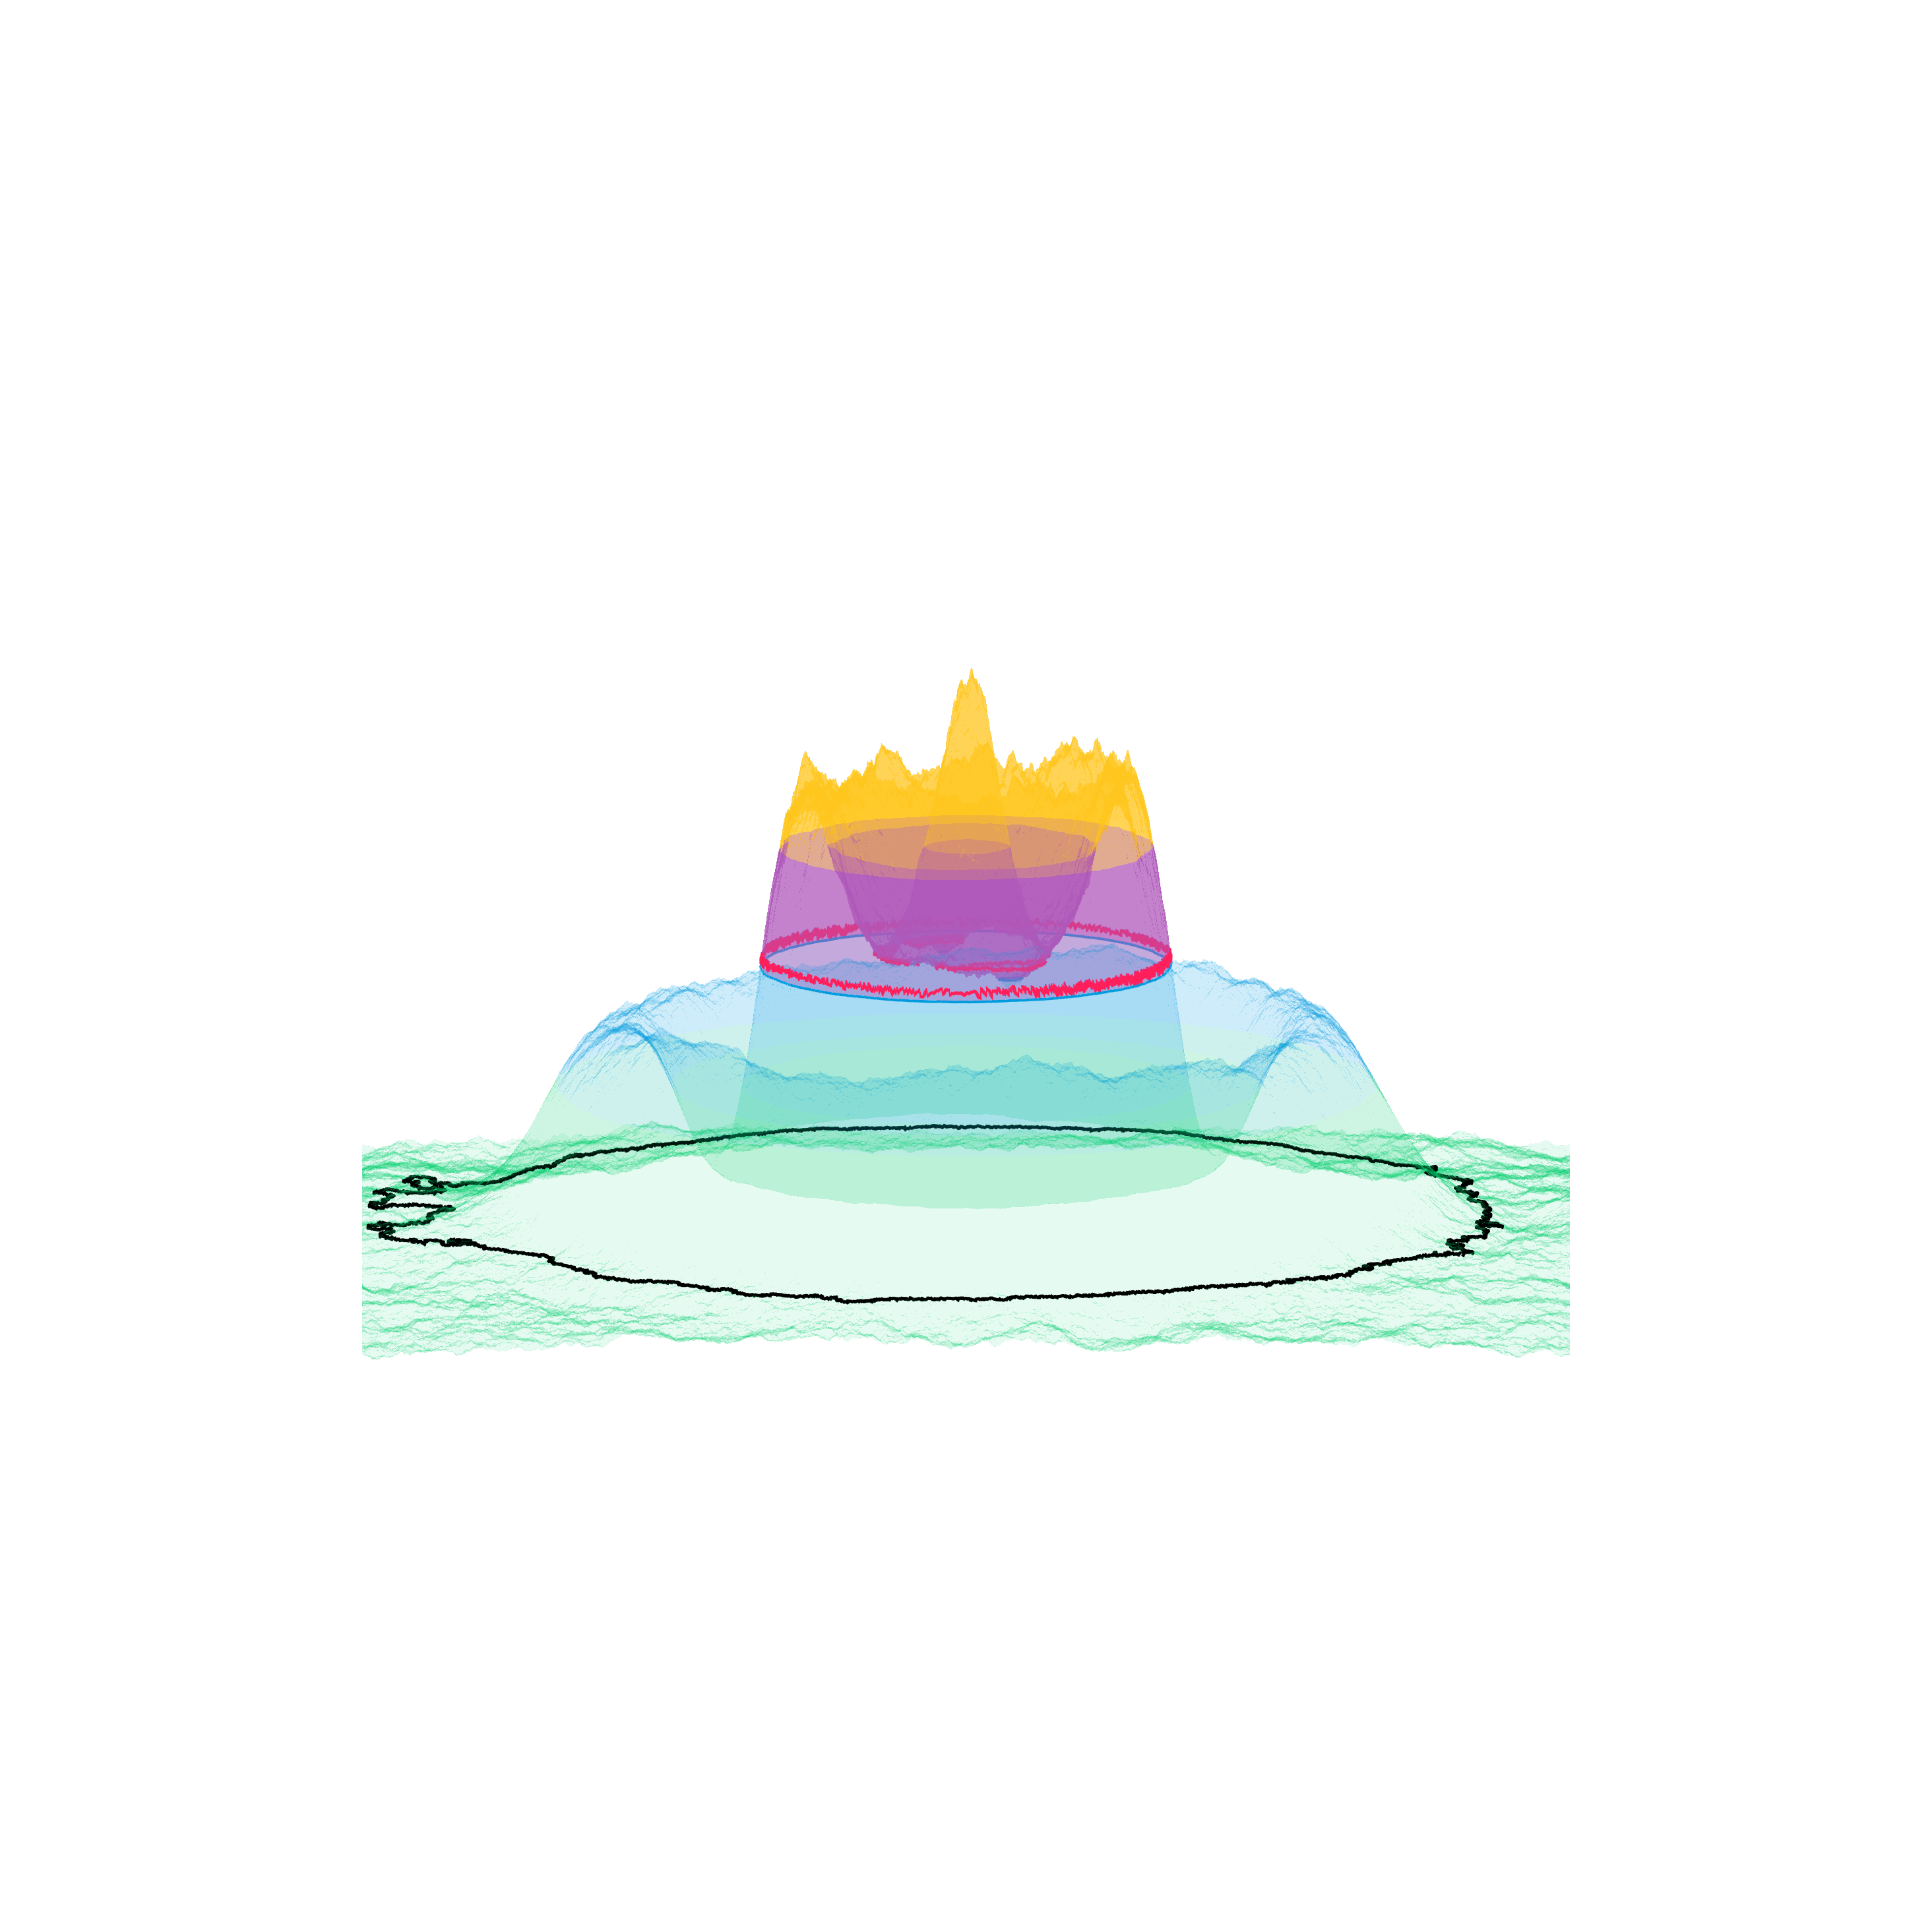
\includegraphics[trim=500 800 500 800, clip, width=0.24\textwidth]{scripts/figures/matching2/surf_side-1_1.png}
  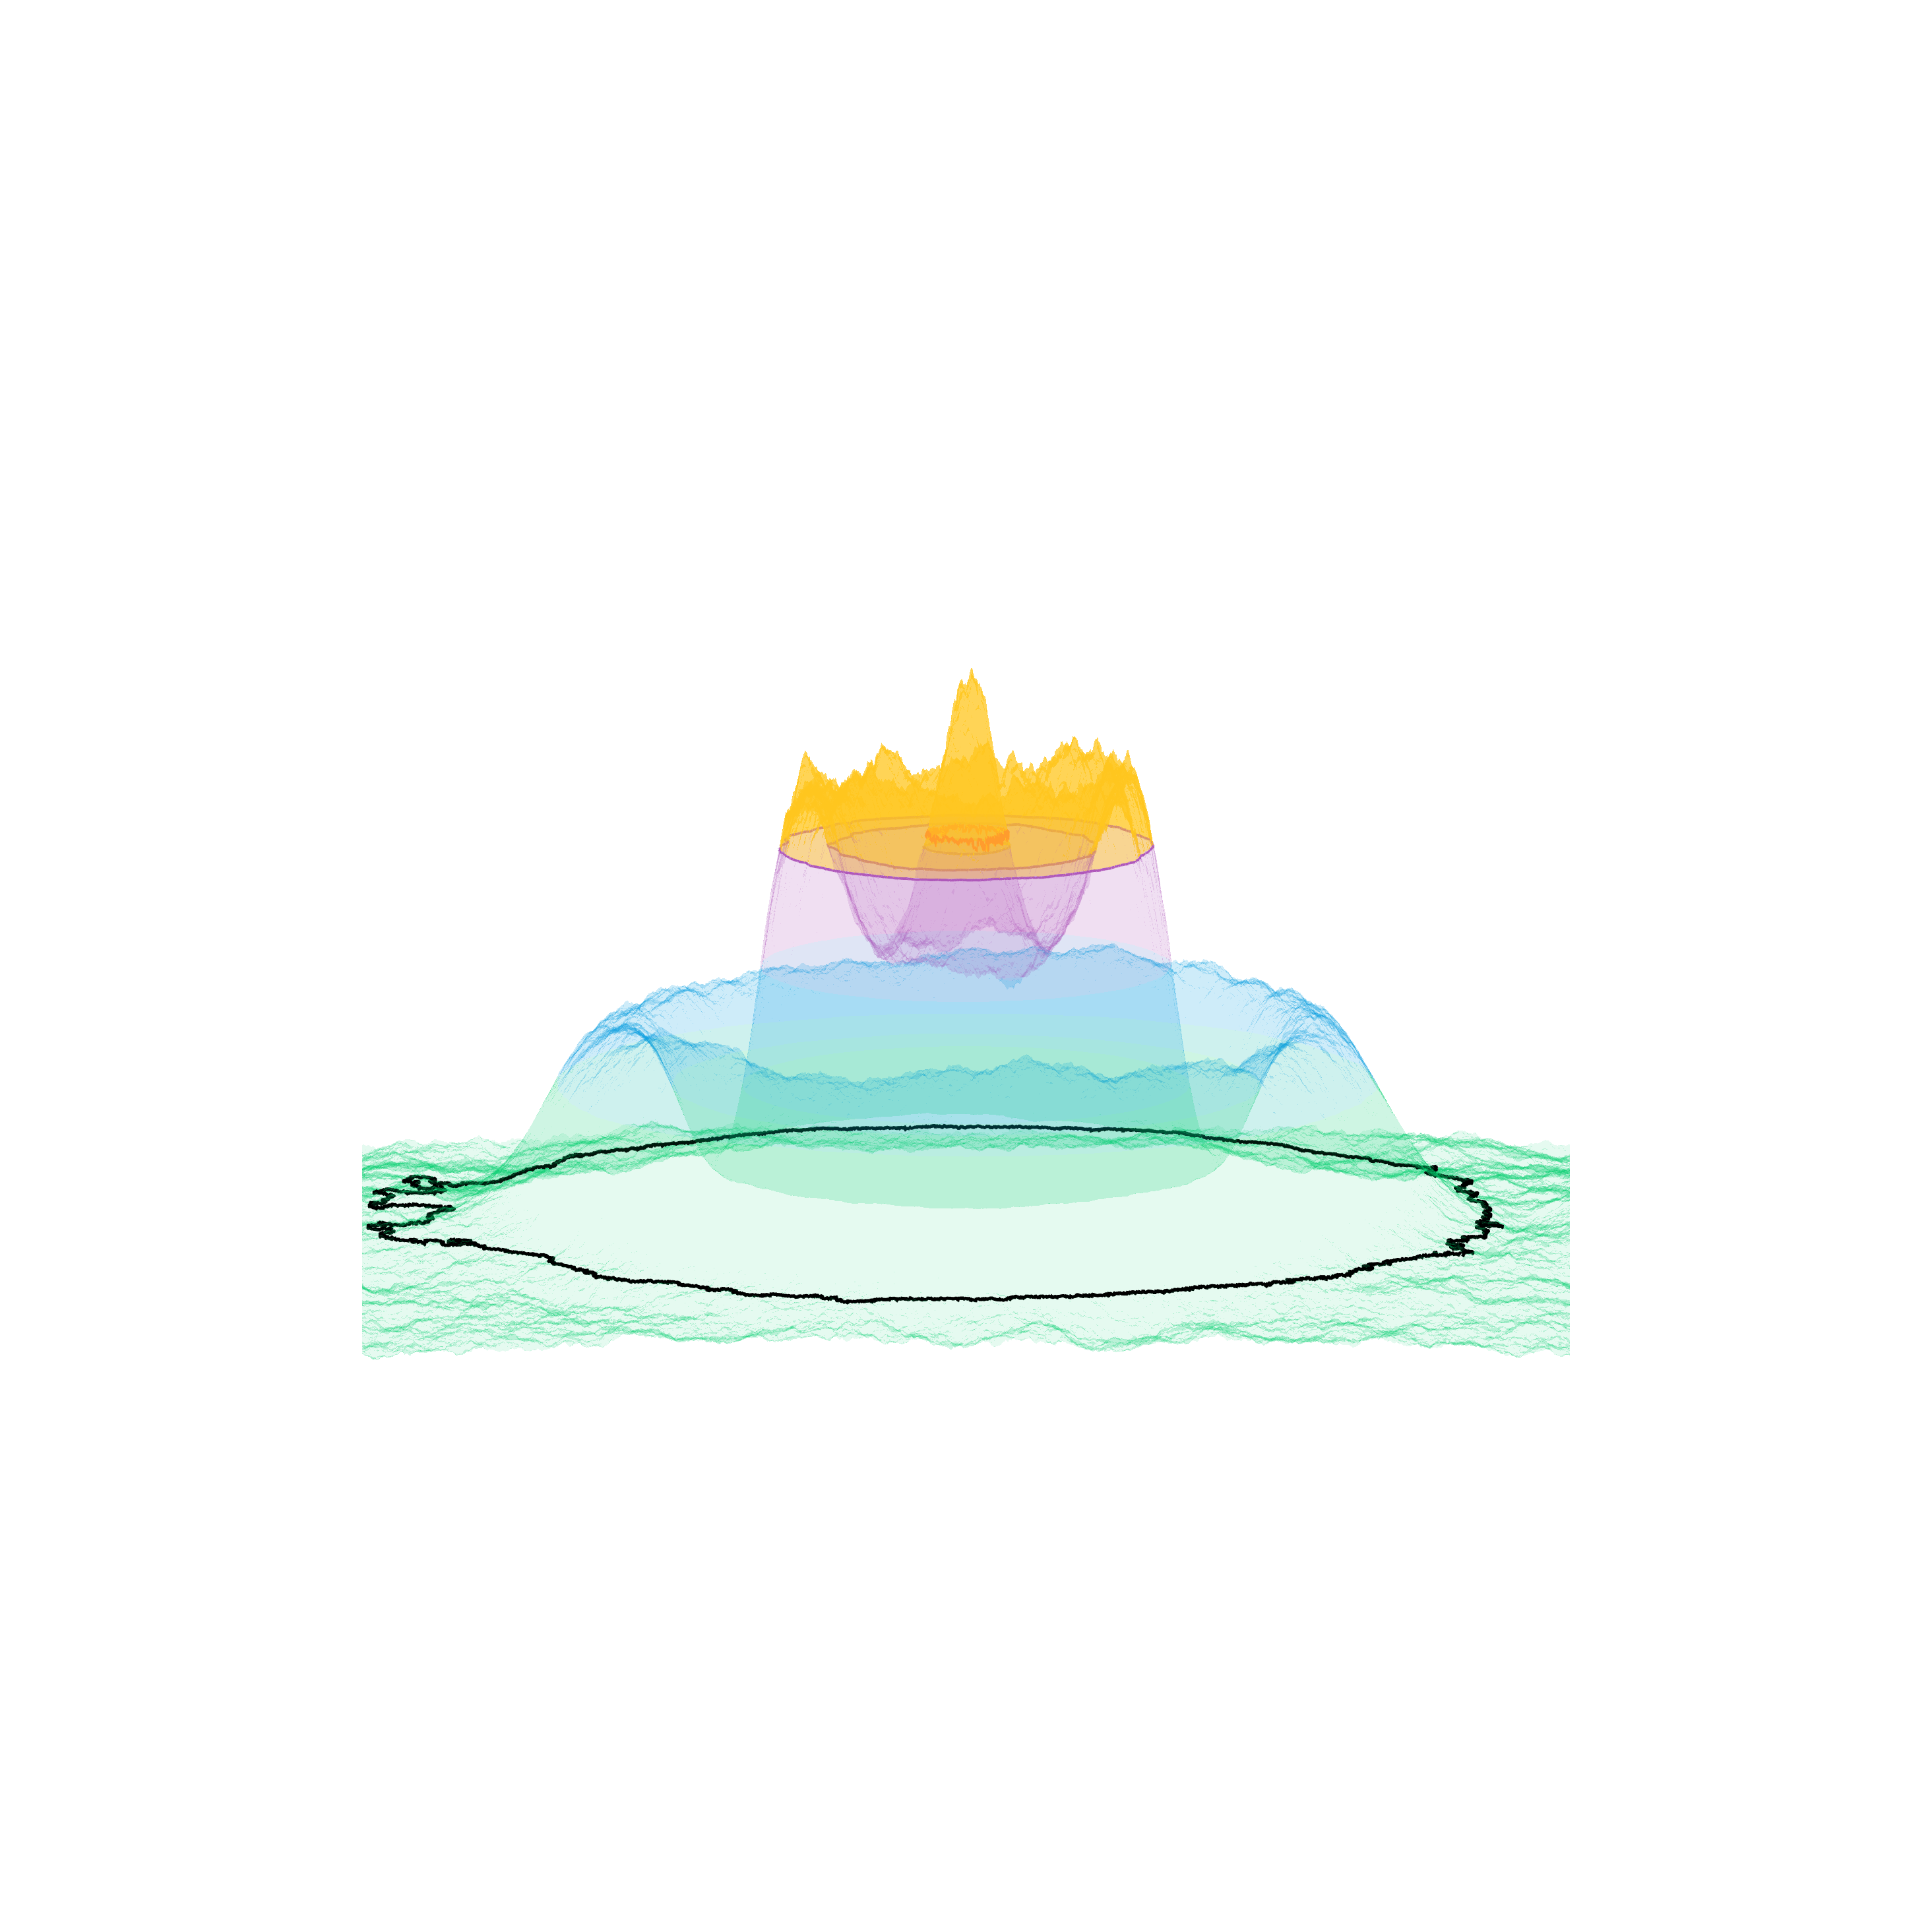
\includegraphics[trim=500 800 500 800, clip, width=0.24\textwidth]{scripts/figures/matching2/surf_side-1_2.png}
  
\includegraphics[trim=500 500 500 500, clip, width=0.24\textwidth]{scripts/figures/matching2/surf_top-1.png}
  
\includegraphics[trim=500 500 500 500, clip, width=0.24\textwidth]{scripts/figures/matching2/surf_top-1_0.png}
  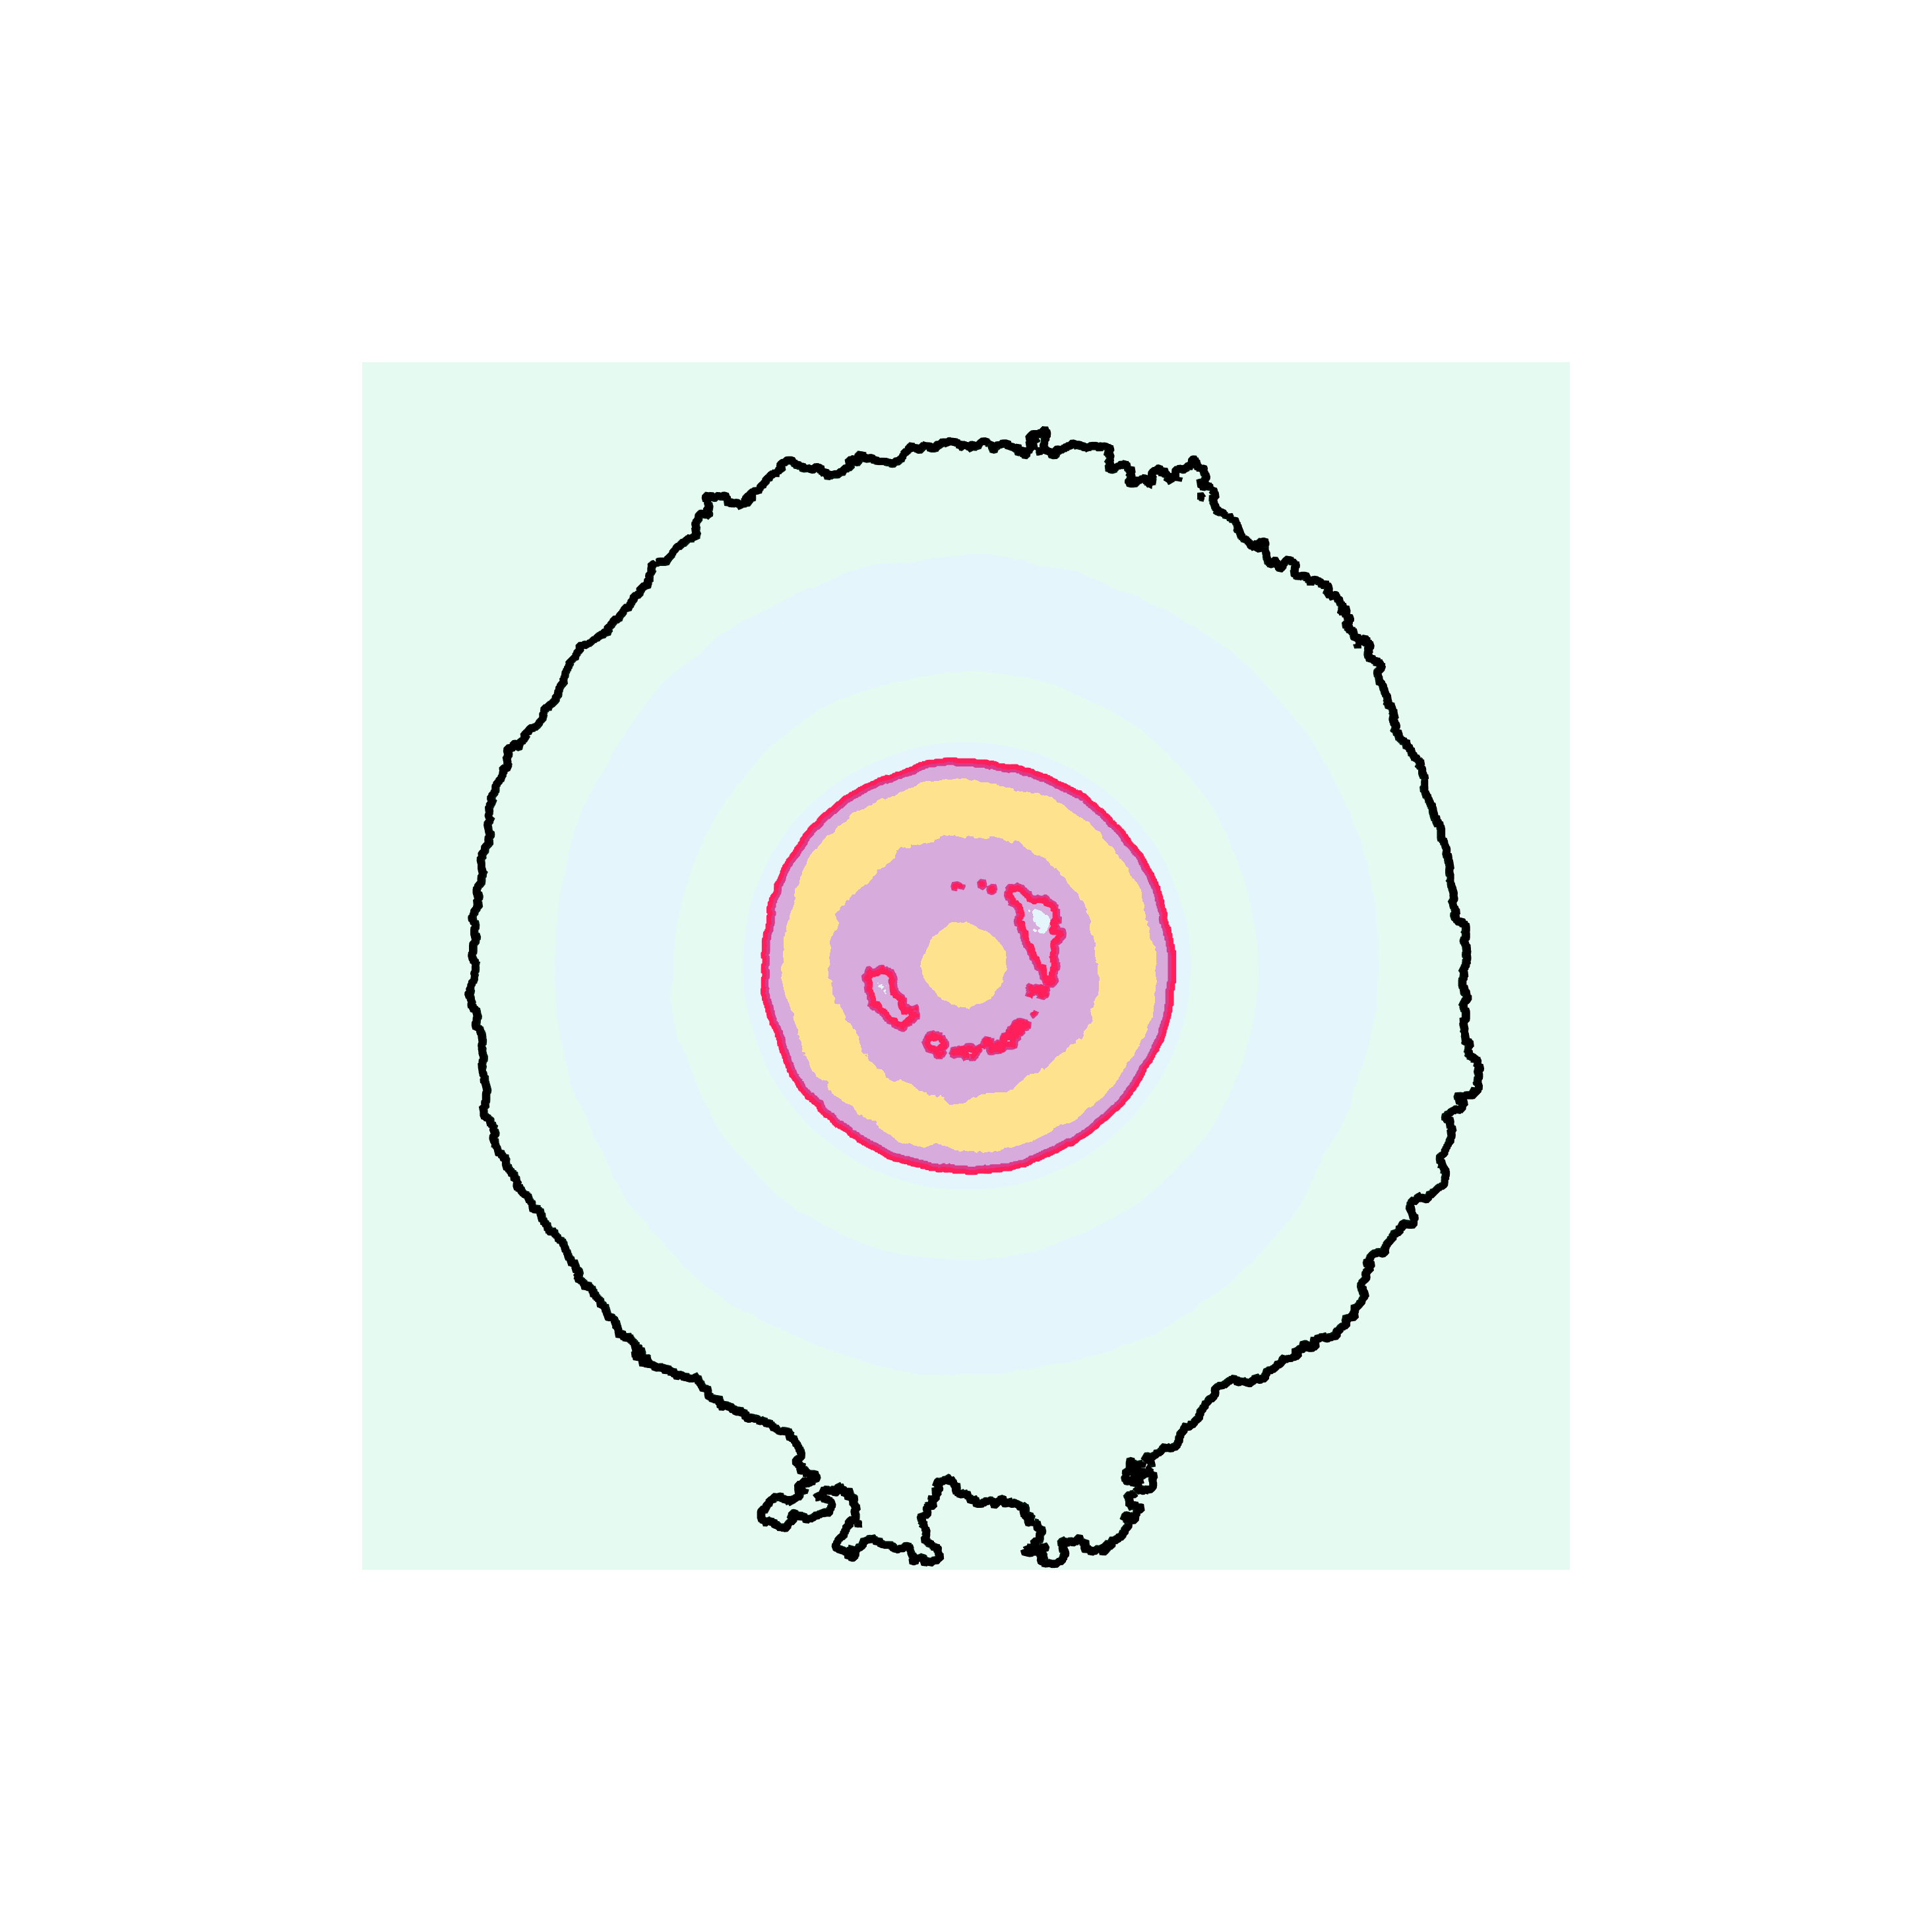
\includegraphics[trim=500 500 500 500, clip, width=0.24\textwidth]{scripts/figures/matching2/surf_top-1_1.png}
  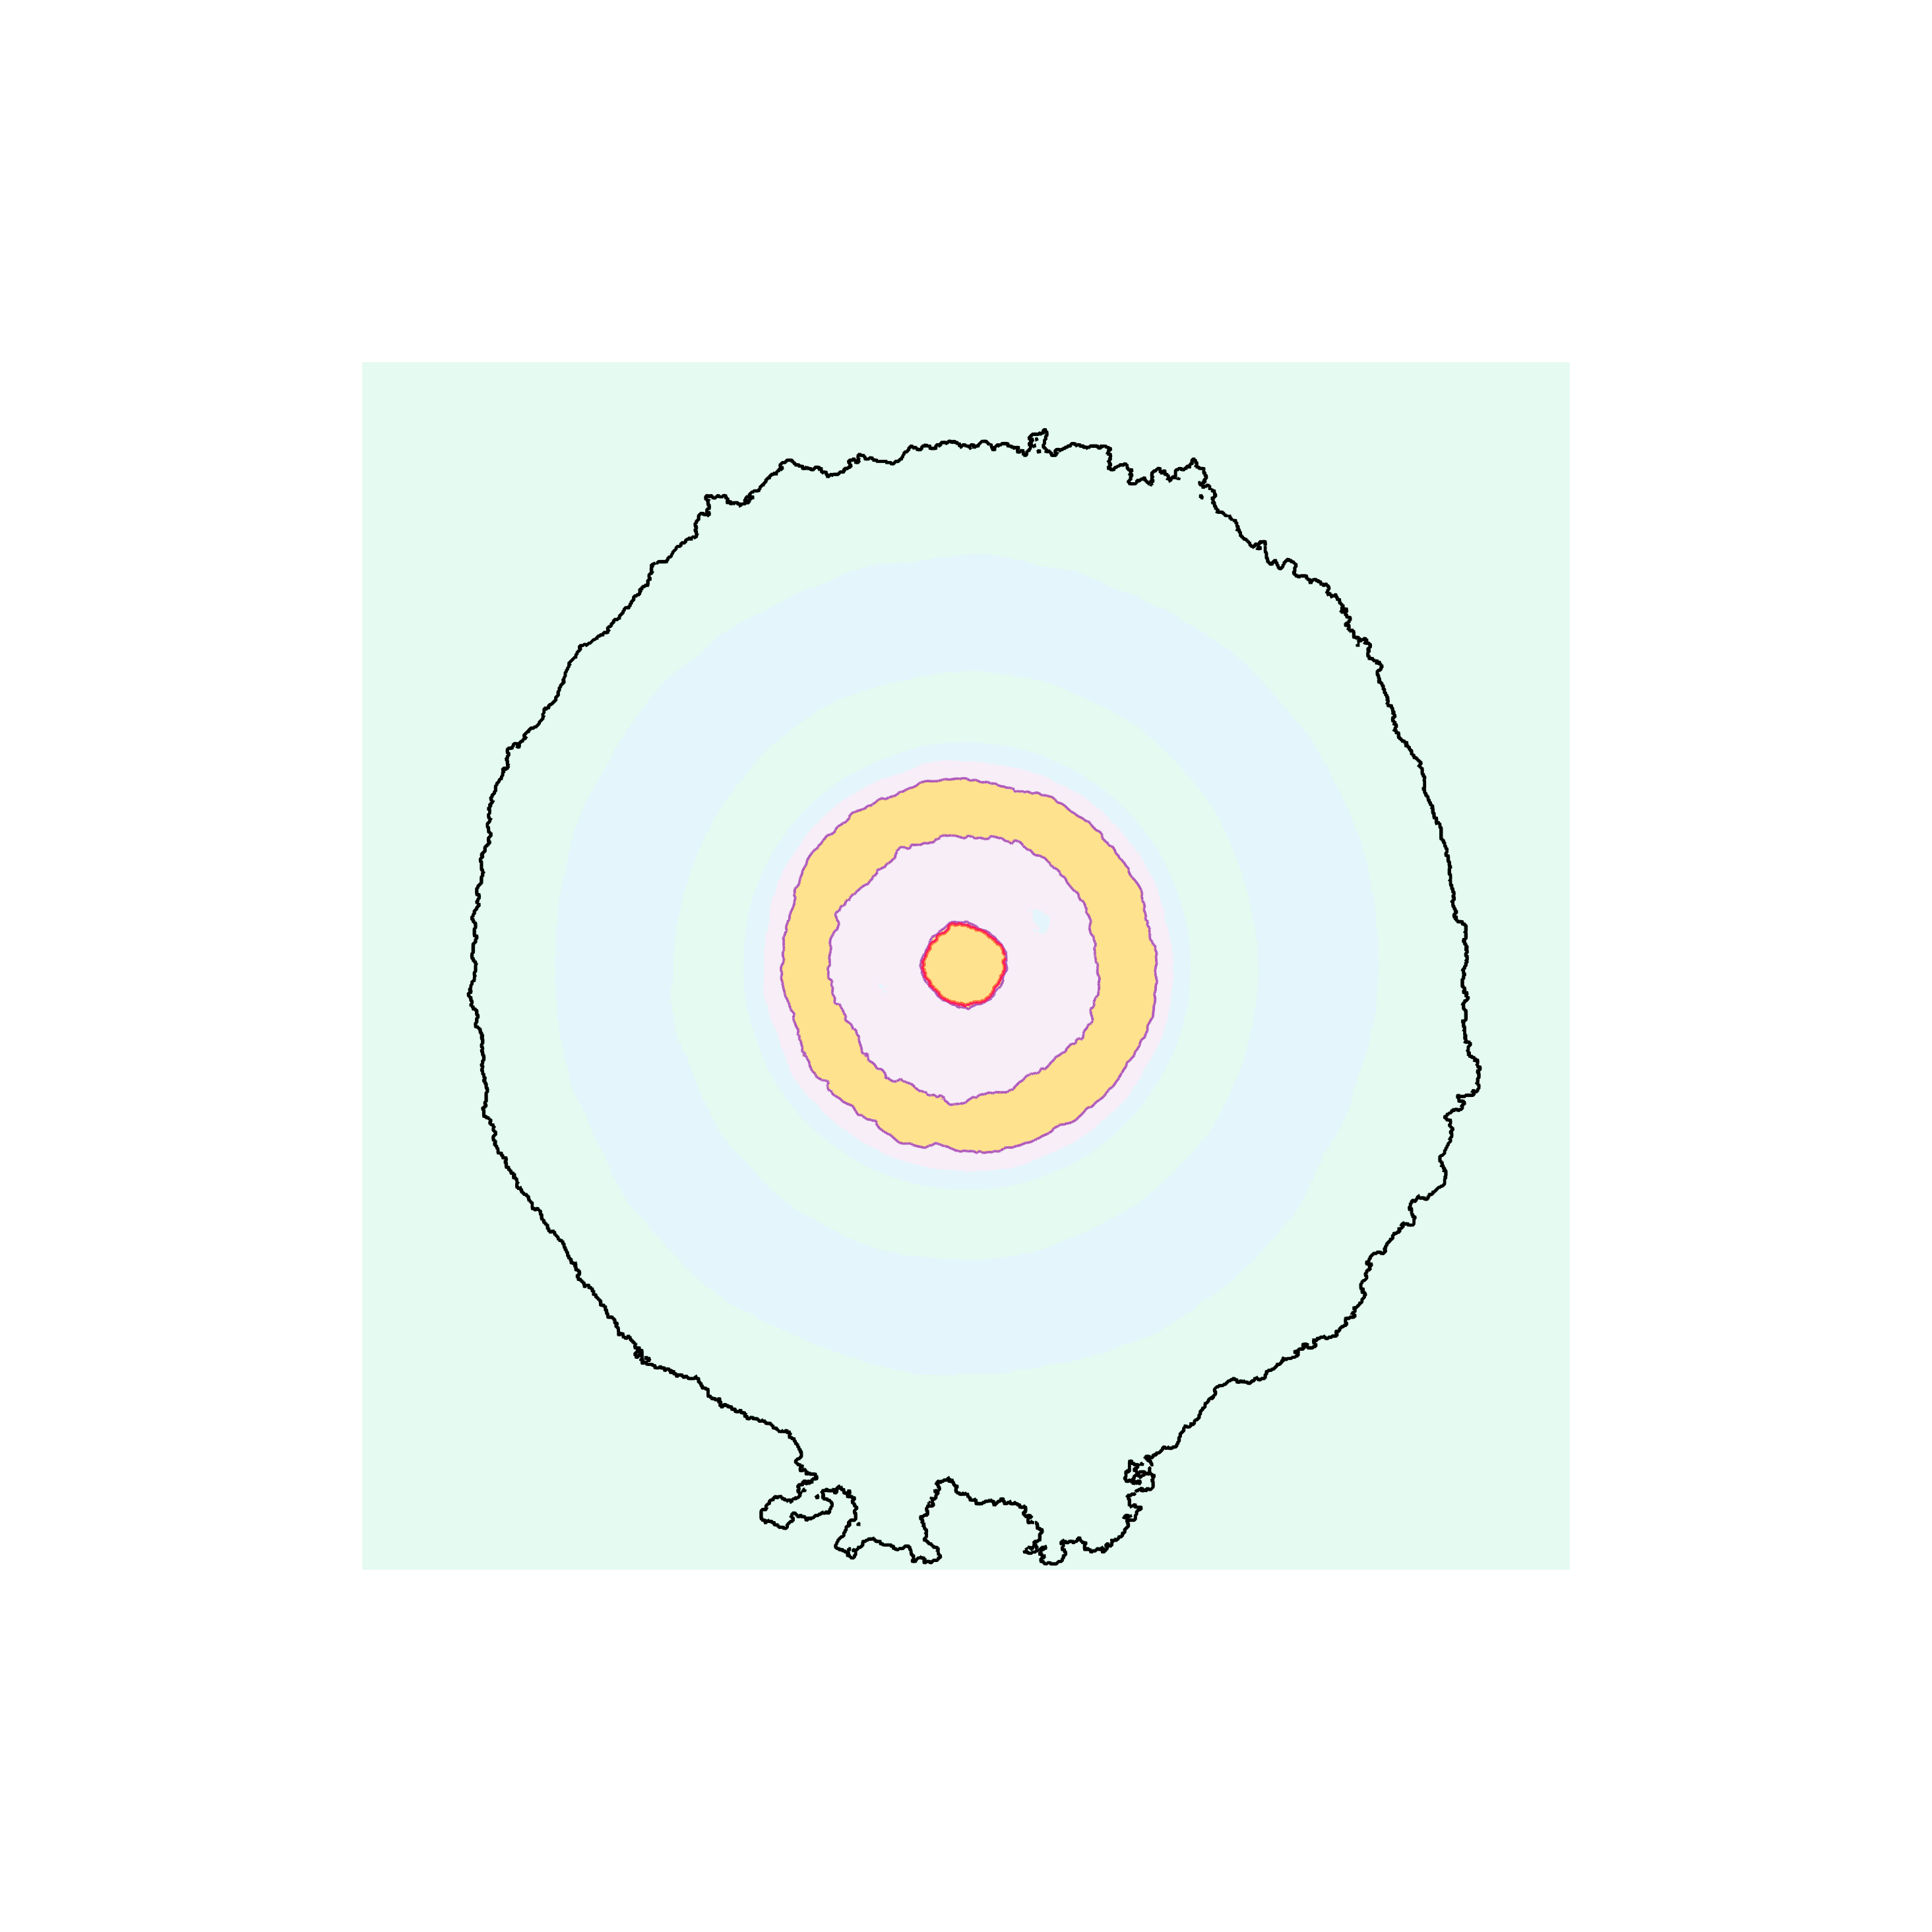
\includegraphics[trim=500 500 500 500, clip, width=0.24\textwidth]{scripts/figures/matching2/surf_top-1_2.png}
  \caption{(Top) $\hom_1$ persistence diagrams of the function depicted in Figure~\ref{fig:ripple1} restricted at $\omega = 0.3, 0.5,$ and $0.7$ (on a $1024\times 1024$ grid).
          The matching is shown between a feature in the full diagram (marked with a diamond) with its representative cycle in black.
          The corresponding representative cycle in the restricted diagram is pictured in red.}
\end{figure}


\clearpage
\bibliographystyle{unsrt}
\bibliography{bibliography}

\clearpage
\appendix
% \section{Misc}\label{apx:misc}
% \subsection{Relative Persistent Nerves}\label{apx:nerves}
% % !TeX root = ../../main.tex

% \subsection{Relative Persistent Nerve Lemma}

\begin{lemma}[\textbf{Persistent Nerve Lemma} (Chazal et. al.~\cite{chazal08towards}, Lemma 3.4)]\label{lem:pers_nerve}
  Let $X\subseteq X'$ be two paracompact spaces, and let $\cU = \{U_i\}_{i\in I}$ and $\mathcal{U}' = \{U_i'\}_{i\in I}$ be good open covers of $X$ and $X'$, respectively, based on some finite parameter set $I$, such that $U_i\subseteq U_i'$ for all $i\in I$.
  Then there exist homotopy equivalences of pairs $\N\cU\to X$ and $\N\cU'\to X'$ that commute with the canonical inclusions $X \hookrightarrow X'$ and $\N\cU\hookrightarrow \N\cU'$ at the homology and homotopy levels.
\end{lemma}

The following lemma is a straightforward application of the Persistent Nerve Lemma to a filtration.

\begin{lemma}\label{lem:pers_nerve_filt}
  Let $X$ be a paracompact space and $\cU = \{U_i\}_{i\in I}$ be a good open covers of $X$ based on some finite parameter set $I$.
  Let $\F = \{F_\alpha\subseteq X\}_{\alpha\in\R}$ be a filtration in $X$ and define $\cU_\alpha := \{X_\alpha\cap U_i\}_{i\in I}$ for all $\alpha\in\R$.
  Then for all $\alpha\leq\beta$ there exist homotopy equivalences of pairs $\N\cU_\alpha\to F_\alpha$ and $\N\cU_\beta\to F_\beta$ that commute with the canonical inclusions $F_\alpha \hookrightarrow F_\beta$ and $\N\cU_\alpha\hookrightarrow \N\cU_\beta$ at the homology and homotopy levels.
\end{lemma}
\begin{proof}
  Because $\cU$ is a good open cover of $X$ we know that $\cU_\alpha$ is a good open cover of $F_\alpha$ for all $\alpha\in\R$.\footnote{\textbf{TODO} prove it.}
  Moreover, because $\F$ is a filtration $F_\alpha\subseteq F_\beta$ for all $\alpha\leq\beta$.
  So $F_\alpha\cap U_i\subseteq X_\beta\cap U_i$ for all $i\in I$, $\alpha\leq\beta$.
  The result therefore follows from Lemma~\ref{lem:pers_nerve}.
\end{proof}

\begin{definition}[Compatible Filtrations (Skraba et. al.~\cite{skraba14approximating})]
  Two filtrations $\A = \{A_\alpha\}$ and $\F = \{F_\alpha\}$ are said to be \textbf{compatible} if for all $\alpha\leq\beta$ the following diagram commutes
  \begin{equation}\label{dgm:compatible}
    \begin{tikzcd}
      A_\alpha\arrow{r}\arrow{d} &
      F_\alpha\arrow{d}\\
      %
      A_\beta\arrow{r} &
      F_\beta.
    \end{tikzcd}
  \end{equation}
  In order to specify an order we will refer to a pair of filtrations $(\F, \A)$ as a \textbf{compatible pair of filtrations}.
\end{definition}

\begin{theorem}[Skraba et. al.~\cite{skraba14approximating}, Theorem 1]\label{thm:rel_interleave}
  If $(\F, \A)$ and $(\F', \A')$ are compatible pairs of filtrations such that the $k$th persistent homology modules of $\F$ and $\F'$ (resp. $\A$ and $\A'$) are $\e$-interleaved then the corresponding relative modules of $\{(F_\alpha, A_\alpha)\}$ and $\{(X_\alpha', Y_\alpha')\}$ are $\e$-interleaved.
\end{theorem}

Because two isomorphic persistence modules are $0$-interleaved we have the following corollary of Theorem~\ref{thm:rel_interleave}.

\begin{corollary}\label{cor:rel_interleave_iso}
  If $(\F, \A)$ and $(\F', \A')$ are compatible pairs of filtrations such that the $k$th persistent homology modules of $\F$ and $\F'$ (resp. $\A$ and $\A'$) are isomorphic then the relative modules $\{(F_\alpha, A_\alpha)\}$ and $\{(X_\alpha', Y_\alpha')\}$ are isomorphic.
\end{corollary}

\begin{lemma}[\textbf{Relative Persistent Nerve Lemma}]\label{lem:rel_pers_nerve}
  Let $X$ be a paracompact space and $Y\subseteq X$.
  Let $\cU = \{U_i\}_{i\in I}$ and $\cV = \{V_i\}_{i\in I}$ be good open covers of $X$ and $Y$, respectively, based on some finite parameter set $I$, such that $V_i\subseteq U_i$ for all $i\in I$.
  Let $\F = \{F_\alpha\}$ be a filtration in $X$ and $A_\alpha := Y\cap F_\alpha$ so that $\A = \{A_\alpha\}$ is a filtration in $Y$.
  Let $\cU_\alpha := \{X_\alpha\cap U_i\}$ and $\cV_\alpha := \{A_\alpha\cap V_i\}$.
  Then the $k$th (relative) persistent homology modules of $\{(F_\alpha, A_\alpha)\}$ and $\{(\N\cU_\alpha, \N\cV_\alpha)\}$ are isomorphic.
\end{lemma}
\begin{proof}
  Because
  \[\N\cU_\alpha = \left\{\bigcap_{i\in S} F_\alpha\cap U_i\mid S\subseteq I\right\} = \{\sigma\cap F_\alpha\}_{\sigma\in \N\cU}\]
  and $F_\alpha\subseteq F_\beta$ for all $\alpha\leq\beta$ we have inclusions $\N\cU_\alpha\hookrightarrow\N\cU_\beta$ for all $\alpha\leq\beta$.
  Similarly, because
  \[\N\cV_\alpha = \{\tau\cap A_\alpha\}_{\tau\in \N\cV} = \{\sigma\cap (Y\cap F_\alpha)\}_{\sigma\in\N\cU}\]
  we have inclusions $\N\cV_\alpha\hookrightarrow\N\cV_\beta$ for all $\alpha\leq\beta$ and, because $V_i\subseteq U_i$ for all $i\in I$, we have inclusions $\N\cV_\alpha\hookrightarrow \N\cU_\alpha$ for all $\alpha\in\R$.
  Letting $\N\cU_\F := \{\N\cU_\alpha\}$ and $\N\cV_\A := \{\N\cV_\alpha\}$ it follows that $(\N\cU_\F, \N\cV_\A)$ is a compatible pair of filtrations.
  Moreover, by Lemma~\ref{lem:pers_nerve_filt}, the following diagrams commute for all $\alpha\leq\beta$.
  \[\begin{tikzcd}
      \N\cU_\alpha \arrow{r}\arrow{d} &
      \N\cU_\beta \arrow{d}\\
      %
      X_\alpha\arrow{r} &
      X_\beta,
    \end{tikzcd}\hspace{10ex}
    \begin{tikzcd}
      \N\cV_\alpha \arrow{r}\arrow{d} &
      \N\cV_\beta \arrow{d}\\
      %
      Y_\alpha\arrow{r} &
      Y_\beta
    \end{tikzcd}\]
  where the horizontal maps are canonical inclusions and vertical maps are homotopy equivalences.
  Letting $\N\U_\F$, $\X_\F$ and $\N\V_\A$, $\Y_\A$ denote the $k$th persistent homology modules of $\N\cU_\F$, $\F$ and $\N\cV_\A$, $\A$, respectively, the homotopy equivalences induce isomorphisms on homology for all $\alpha\in\R$, which constitute isomorphisms of persistence modules.
  % the following isomorphisms of persistence modules
  % \[ \N_\F\in\Hom(\N\U_\F, \X_\F),\text{ and } \N_\A\in\Hom(\N\V_\A,\Y_\A).\]
  % \[ \N_\F := \{n_{\cU_\alpha} : \hom_k(\N\cU_\alpha)\to \hom_k(F_\alpha)\}\in\Hom(\N\U_\F, \X_\F),\text{ and }\]
  % \[ \N_\A : = \{n_{\cV_\alpha} : \hom_k(\N\cV_\alpha)\to \hom_k(A_\alpha)\}\in\Hom(\N\V_\A,\Y_\A).\]
  The result therefore follows from Corollary~\ref{cor:rel_interleave_iso}.
\end{proof}

% \begin{lemma}[Persistent Nerve Lemma]\label{lem:rel_pers_nerve}% (Lemma 3.4, Chazal~\cite{chazal08towards})]\label{lem:rel_pers_nerve}
%   Let $X\subseteq X'$ be two paracompact spaces and $Y\subseteq Y'$ be two subspaces $Y\subseteq X$, $Y'\subseteq X'$.
%   Let $\mathcal{U} = \{U_a\}_{a\in A}$ and $\mathcal{U}' = \{U_a'\}_{a\in A}$ be good open covers of $X$ and $X'$, respectively, such that $U_a\subseteq U_a'$ for all $a\in A$.
%   Let $\cV = \{V_a\}_{a\in A} \subseteq \mathcal{U}$ and $\cV' = \{V_a'\}_{a\in A}\subseteq \mathcal{U}'$ be good open subcovers of $Y$ and $Y'$, respectively, such that $V\subseteq V'$ for all $a\in A$.
%   Then there exist homotopy equivalences of pairs $(\N\mathcal{U}, \N\cV)\to (X, Y)$ and $(\N\mathcal{U}', \N\cV')$ that commute with the canonical inclusions of pairs $(X, Y)\hookrightarrow (X', Y')$ and $(\N\mathcal{U}, \N\cV)\hookrightarrow (\N\mathcal{U}', \N\cV')$ at the homology and homotopy levels.
% \end{lemma}

% \begin{theorem}[Alexander Duality]\label{thm:alexander}
%   If $D$ is a compact, locally contractible, nonempty, proper subspace of $S^d$ then for all $k$ there is an isomorphism
%   \[ \Gamma_D^k : \tilde{\hom}_k(D)\to \tilde{\hom}^{d-k-1}(S^d\setminus D). \]
%
%   If $(D, B)$ is a pair of such subspaces of $S^d$ then for all $k$ there is an isomorphism
%   \[ \Gamma_{(D,B)}^k : \tilde{\hom}_k(D, B)\to \tilde{\hom}^{d-k}(S^d\setminus B, S^d\setminus D). \]
% \end{theorem}

% \begin{lemma}[Lemma 3.2 from~\cite{chazal08towards}]\label{lem:sandwich}
%     Given a sequence $A\to B\to C\to D\to E\to F$ of homomorphisms between finite-dimensional vector spaces, if $\rk(A\to F) = \rk(C\to D)$ then this quantity also equals the rank of $B\to E$.
%     Similarly, if $A\to B\to C\to E\to F$ is a sequence of homomorphisms such that $\rk(A\to F) = \dim~C$ then $\rk(B\to E) = \dim~C$.
% \end{lemma}

% \subsection{What we need from $X$, $D$, and $P$}
%
% Let $\X$ be a compact Riemannian $d$-manifold and let $D$ be a compact subset of $\X$ and let $\dist(x, y) = \|x - y\|$ denote the distance between points $x,y\in D$ as a subspace of $\X$.
% For $A\subset D$ and $x\in D$ let
% \[\dist_A(x) = \min_{a\in A}\dist(x, a)\]
% denote the distance from $x$ to the set $A$.
% We will use open metric balls restricted to $D$ with the subspace topology
% \[\ball_D^\e(x) = \{y\in D\mid \dist(x, y) < \e\}\]
% and offsets
% \[A^\e = \{x\in D\mid \dist_A(x) < \e\}.\]
%
% A ball $\ball_D^\e(x)$ is said to be \textbf{strongly convex} if for each pair of points $y,z$ in the closure of $\ball_D^\e(x)$ there exists a unique shortest path in $D$ between $y$ and $z$, and the interior of this path is included in $\ball_D^\e(x)$.
% Let $\varrho_D(x)$ be the supremum of the radii such that $\ball_D^\e(x)$ is strongly convex.
% The \textbf{strong convexity radius} of $D$ is defined
% \[ \varrho_D := \inf_{x\in D} \varrho_D(x).\]
% Note that this value is positive for compact $D$.
%
% We will require that, for some $\zeta > 0$, $D$ is a compact subspace of $\X$ with strong convexity radius $\varrho_D > 2\zeta$.
% For a finite point set $P$ such that $P^{2\delta}\subset \intr_\X(D)$ and any subset $Q\subseteq P$ we will assume that $D\setminus Q^\delta,$ and $D\setminus P^\delta$ are locally path connected for some $\delta > 0$.
%
% % \begin{lemma}
% %   If $Q\subseteq R\subseteq P$ then
% %   \[ \rk~\hom_d((P^\delta, Q^\delta)\hookrightarrow (P^{2\delta}, R^{\delta})) = \rk~\hom_0((D\setminus R^{\delta}, D\setminus P^{\delta})\hookrightarrow(D\setminus Q^\delta, D\setminus P^\delta)).\]
% % \end{lemma}
%
% \begin{lemma}
%   For any $Q\subseteq R\subseteq P$
%   \[\rk~\hom_d(\rips^\delta(P, Q)\hookrightarrow \rips^{2\delta}(P, R))\leq \rk~\hom_0((D\setminus R^{\delta}, D\setminus P^{\delta})\hookrightarrow (D\setminus Q^\delta, D\setminus P^\delta)).\]
% \end{lemma}


\section{Duality}\label{apx:duality}
% !TeX root = ../../main.tex

% \subsection{Duality}

For a pair $(A, B)$ in a topological space $X$ and any $R$ module $G$ let $\hom^k(A, B; G)$ denote the \textbf{singular cohomology} of $(A,B)$ (with coefficients in $G$) as a vector space.
Let $\hom^k_c(A, B; G)$ denote the corresponding \textbf{singular cohomology with compact support}, where $\hom^k_c(A, B; G)\cong \hom^k(A, B; G)$ for any compact pair $(A,B)$.

The following corollary follows from the Universal Coefficient Theorem for singular homology (and cohomology) as vector spaces over a field $\FF$, as the dual vector space $\Hom(\hom_k(A, B), \FF)$ is isomorphic to $\hom_k(A, B; \FF)$ for any finitely generated $\hom_k(A, B)$.\footnote{Reference/verify.}

\begin{corollary}\label{cor:univ_coef}
  For a topological pair $(A, B)$ and a field $\FF$ such that $\hom_0(A, B)$ is finitely generated there is a natural isomorphism
  \[\nu : \hom^0(A, B; \FF)\to \hom_0(A, B; \FF).\]
\end{corollary}

Let $\overline{\hom}^k(A, B; G)$ be the \textbf{Alexander-Spanier cohomology} of the pair $(A,B)$, defined as the limit of the direct system of neighborhoods $(U,V)$ of the pair $(A, B)$.
Let $\overline{\hom}^k_c(A, B; G)$ denote the corresponding \textbf{Alexander-Spanier cohomology with compact support} where $\overline{\hom}^k_c(A, B; G)\cong\overline{\hom}^k(A, B; G)$ for any compact pair $(A, B)$.

\begin{theorem}[\textbf{Alexander-Poincar\'e-Lefschetz Duality} (Spanier, Theorem 6.2.17)]\label{thm:alexander}
  Let $X$ be an orientable $d$-manifold and $(A, B)$ be a compact pair in $X$.
  Then for all $k$ and $R$ modules $G$ there is a (natural) isomorphism
  \[\lambda : \hom_k(X\setminus B, X\setminus A; G)\to \overline{\hom}^{d-k}(A, B; G).\]
\end{theorem}

A space $X$ is said to be \textbf{homologically locally connected in dimension $n$} if for every $x\in X$ and neighborhood $U$ of $x$ there exists a neighborhood $V$ of $x$ in $U$ such that $\tilde{\hom}_n(V)\to\tilde{\hom}_n(U)$ is trivial for $k\leq n$.

\begin{lemma}[Spanier p. 341, Corollary 6.9.6]\label{lem:alexander_iso}
  Let $A$ be a closed subset, homologically locally connected in dimension $n$, of a Hausdorff space $X$, homologically locally connected in dimension $n$.
  If $X$ has the property that every open subset is paracompact, $\mu : \overline{\hom}_c^k(X,A; G)\to \hom_c^k(X, A; G)$ is an isomorphism for $k\leq n$ and a monomorphism for $q = n+1$.
\end{lemma}

In the following we will assume homology (and cohomology) over a field $\FF$.

\begin{lemma}\label{cor:alexander_iso}
  Let $X$ be an orientable $d$-manifold and $(A,B)$ a compact pair of locally path connected subspaces in $X$.
  Then
  \[\xi : \hom_d(X\setminus B, X\setminus  A)\to \hom_0(A, B)\]
  is a natural isomorphism.
\end{lemma}
\begin{proof}
  Because $X$ is orientable and $(A,B)$ are compact $\lambda : \hom_d(X\setminus B, X\setminus A)\to \overline{\hom}^{0}(A, B)$ is an isomorphism by Theorem~\ref{thm:alexander}.
  Note that
  Moreover, because every subset of $X$ is (hereditarily) paracompact every open set in $A$, with the subspace topology, is paracompact.
  For any neighborhood $U$ of a point $x$ in a locally path connected space there must exist some neighborhood $V\subset U$ of $x$ that is path connected in the subspace topology.
  As $\tilde{\hom}_0(V) = 0$ for any nonempty, path connected topological space $V$ (see Spanier p. 175, Lemma 4.4.7) it follows that $A$ (resp. $B$) are homologically locally connected in dimension $0$.
  Because $(A,B)$ is a compact pair the singular and Alexander-spanier cohomology modules of $(A,B)$ with compact support are isomorphic to those without, thus $\mu:\overline{\hom}^{0}(A, B)\to \hom^0(A, B)$ is an isomorphism.
  By Corollary~\ref{cor:univ_coef} we have a natural isomorphism $\nu : \hom^0(A, B)\to\hom_0(A, B)$ thus the composition $\xi := \nu\circ\mu\circ\lambda : \hom_d(X\setminus B, X\setminus  A)\to \hom_0(A, B)$ is a natural isomorphism.
\end{proof}


% % \begin{theorem}[\textbf{Alexander-Poincar\'e Duality} (Julian et. al.~\cite{julian83alexander}, Theorem 5.1)]\label{thm:alexander}
% %   Let $K$ be an abstract simplicial complex that is a combinatorial oriented $d$-manifold.
% %   Let $L$ be a subcomplex of some refinement of $K$ and $M$ be a subcomplex of $L$.
% %   Let $\overline{L}$ and $\overline{M}$ denote the complements of $L$ and $M$ as subcomplexes of $K$ that do not share vertices with the original complexes.
% %   Then for all $k$ there is a natural isomorphism
% %   \[ \hom^k(L, M)\to \hom_{d-k}(\overline{M},\overline{L}). \]
% % \end{theorem}
%
% % \begin{corollary}
% %   Let $X$ be a topological space and $D$ be a compact subspace of $X$.
% %   Let $(U, V)$ be a topological pair of spaces in $D$ and suppose there exists a triangulation $\Delta X$ of $X$ such that there exists triangulation $\Delta U$ of $U\subset$ that is a subcomplex of some refinement of $\Delta X$ and a triangulation $\Delta V$ of $V$ that is a subcomplex of $\Delta U$.
% %   Then for all $k$ there is a natural isomorphism
% %   \[ \hom^k(U, V)\to\hom_{d-k}(D\setminus U, D\setminus V).\]
% % \end{corollary}
%
%
% \begin{corollary}\label{cor:univ_coef}
%   Let $(A, B)$ be a topological pair and $\FF$ be a field such that $\hom_k(A, B; \FF)$ is finitely generated.
%   Then there is a natural isomorphism
%   \[\hom^k(A, B; \FF)\to \hom_k(A, B; \FF).\]
% \end{corollary}
% \begin{proof}
%   As $\mathrm{Ext}(\Hom(A, B), \FF) = 0$ for any field $\FF$ the map
%   \[\hom^k(A, B; \FF)\to \Hom(\hom_k(A, B), \FF)\]
%   in the natural short exact sequence provided by Theorem~\ref{thm:univ_coef} is a natural isomorphism.
%   The result follows from the fact that $\hom_k(A, B; \FF)$ is finitely generated, and is therefore isomorphic to the dual vector space $\Hom(\hom_k(A, B), \FF)$.
% \end{proof}
%
% % \begin{theorem}[\textbf{Universal Coefficient Theorem} (Munkres p. 337, Corollary 56.4)]\label{thm:univ_coef}
% %   Let $(A,B)$ be a topological pair such that $\hom_k(A, B)$ is finitely generated for all $k$.
% %   Then for all $k$ and any abelian group $G$ there is a natural exact sequence
% %   \[ 0\to\mathrm{Ext}(\hom^{k+1}(A, B), G)\to \hom_k(A, B; G)\to \Hom(\hom^k(A, B), G)\to 0.\]
% %   This sequence splits, but not naturally.
% % \end{theorem}
%
% \begin{theorem}
%   Let $X$ be a topological space and $D$ be a compact subspace of $X$.
%   Suppose there exists a triangulation $\Delta X$ of $X$ that is a combinatorial oriented $d$-manifold.
%   Let $(U, V)$ be a topological pair of spaces in $D$ and $\FF$ be a field such that $\hom_k(U,V;\FF)$ is finitely generated for all $k$.
%
%   If there exists a pair of triangulations $(\Delta U, \Delta V)$ of the pair $(U, V)$ such that $\Delta U$ is a subcomplex of some refinement of $\Delta X$ then there is a natural isomorphism
%   \[ \hom_d(U, V; \FF)\to \hom_0(X\setminus V, X\setminus U; \FF).\]
% \end{theorem}
% \begin{proof}
%   By Theorem~\ref{thm:alexander} we have a natural isomorphism
%   \[ \hom^d(\Delta U, \Delta V; \FF)\to \hom_{0}(\overline{\Delta V}, \overline{\Delta U}; \FF) \]
%   where $\overline{\Delta V}$ and $\overline{\Delta U}$ denote the complements of $\Delta V$ and $\Delta U$ as subcomplexes of $\Delta X$ that do not share vertices with their respective original complexes.
%   \textbf{TODO}\footnote{$\hom^d(U, V;\FF)\cong \hom^d(\Delta U, \Delta V;\FF),\ \hom_{0}(\overline{\Delta V}, \overline{\Delta U}; \FF) \cong \hom_0(X\setminus V, X\setminus U; \FF).$}
%
%   Because $\hom_d(U, V; \FF)$ is finitely generated $\hom_d(U, V;\FF)\cong\hom^d(U, V; \FF)$ by Corollary~\ref{cor:univ_coef}.
%   It follows that the composition
%   \[\hom_d(U, V; \FF)\to \hom^d(U,V;\FF)\to\hom_0(X\setminus V, X\setminus U; \FF)\]
%   is a natural isomorphism as desired.
% \end{proof}
% % \begin{proof}
% %   \begin{itemize}
% %     \item By Theorem~\ref{thm:univ_coef} we have a short exact sequence
% %       \[ 0\to\mathrm{Ext}(\hom^{d+1}(\Delta U, \Delta V), G)\to \hom_d(\Delta U, \Delta V; G)\to \Hom(\hom^d(\Delta U, \Delta V), G)\to 0\]
% %       for any abelian group $G$.
% %       Because $\Delta U,\Delta V$ are subcomplexes of the combinatorial $d$-manifold $\Delta X$, $\hom^{d+1}(\Delta U, \Delta V) = 0$, so $\hom_d(\Delta U, \Delta V; G)\to \Hom(\hom^d(\Delta U, \Delta V), G)$ is an isomorphism.
% %     \item By Theorem~\ref{thm:alexander} we have a natural isomorphism $\hom^d(\Delta U, \Delta V)\to \hom_0(\overline{\Delta V},\overline{\Delta U})$.
% %       Therefore, because we have natural\footnote{\textbf{TODO} natural short exact $\implies$ natural isomorphism.} isomorphisms $\hom_d(\Delta U, \Delta V; G)\to \Hom(\hom^d(\Delta U, \Delta V), G)$ for all abelian groups $G$, we have a natural isomorphism (\textbf{TODO} prove it).
% %       \[\hom_d(\Delta U, \Delta V)\to \hom_0(\overline{\Delta V},\overline{\Delta U}).\]
% %     \item Because $\hom_d(U, V)\cong \hom_d(\Delta U, \Delta V)$ and $\hom_0(X\setminus V, X\setminus U)\cong \hom_0(\overline{\Delta V},\overline{\Delta U})$ (\textbf{TODO} prove it\footnote{$(X\setminus V, X\setminus U)$ or $(D\setminus V, D\setminus U)$?}), we have a natural isomorphism
% %     \[ \hom_d(U, V)\to \hom_0(X\setminus V, X\setminus U). \]
% %   \end{itemize}
% % \end{proof}
%
%
% %
% % \begin{theorem}[\textbf{Alexander Duality} (Spanier p. 296, Theorem 6.2.17)]
% %   Let $U$ be an orientation over $R$ of an $d$-manifold $X$ and let $(A, B)$ be a compact pair in $X$.
% %   Then for all $k$ and $R$ modules $G$ there is a natural isomorphism
% %   \[ \hom_k(X\setminus B, X\setminus A; G)\to\overline{\hom}^{d-k}(A, B; G).\]
% % \end{theorem}
% %
% % \begin{lemma}
% %   Let $U$ be an orientation over $R$ of an $d$-manifold $X$ and let $(A, B)$ be a compact pair in $X$ such that $\hom_k(A, B)$ is finitely generated for all $k$.
% %   Then for all $R$ modules $G$ there is a natural isomorphism
% %   \[ \hom_0(X\setminus B, X\setminus A; G)\to\hom_d(A, B; G). \]
% % \end{lemma}
% % \begin{proof}
% %   \textbf{TODO}
% % \end{proof}


\section{Omitted Proofs}\label{apx:omit}
\printproofs

\section{Additional Figures}\label{apx:extra}
% !TeX root = ../../main.tex

\begin{figure}[htbp]
  \centering
  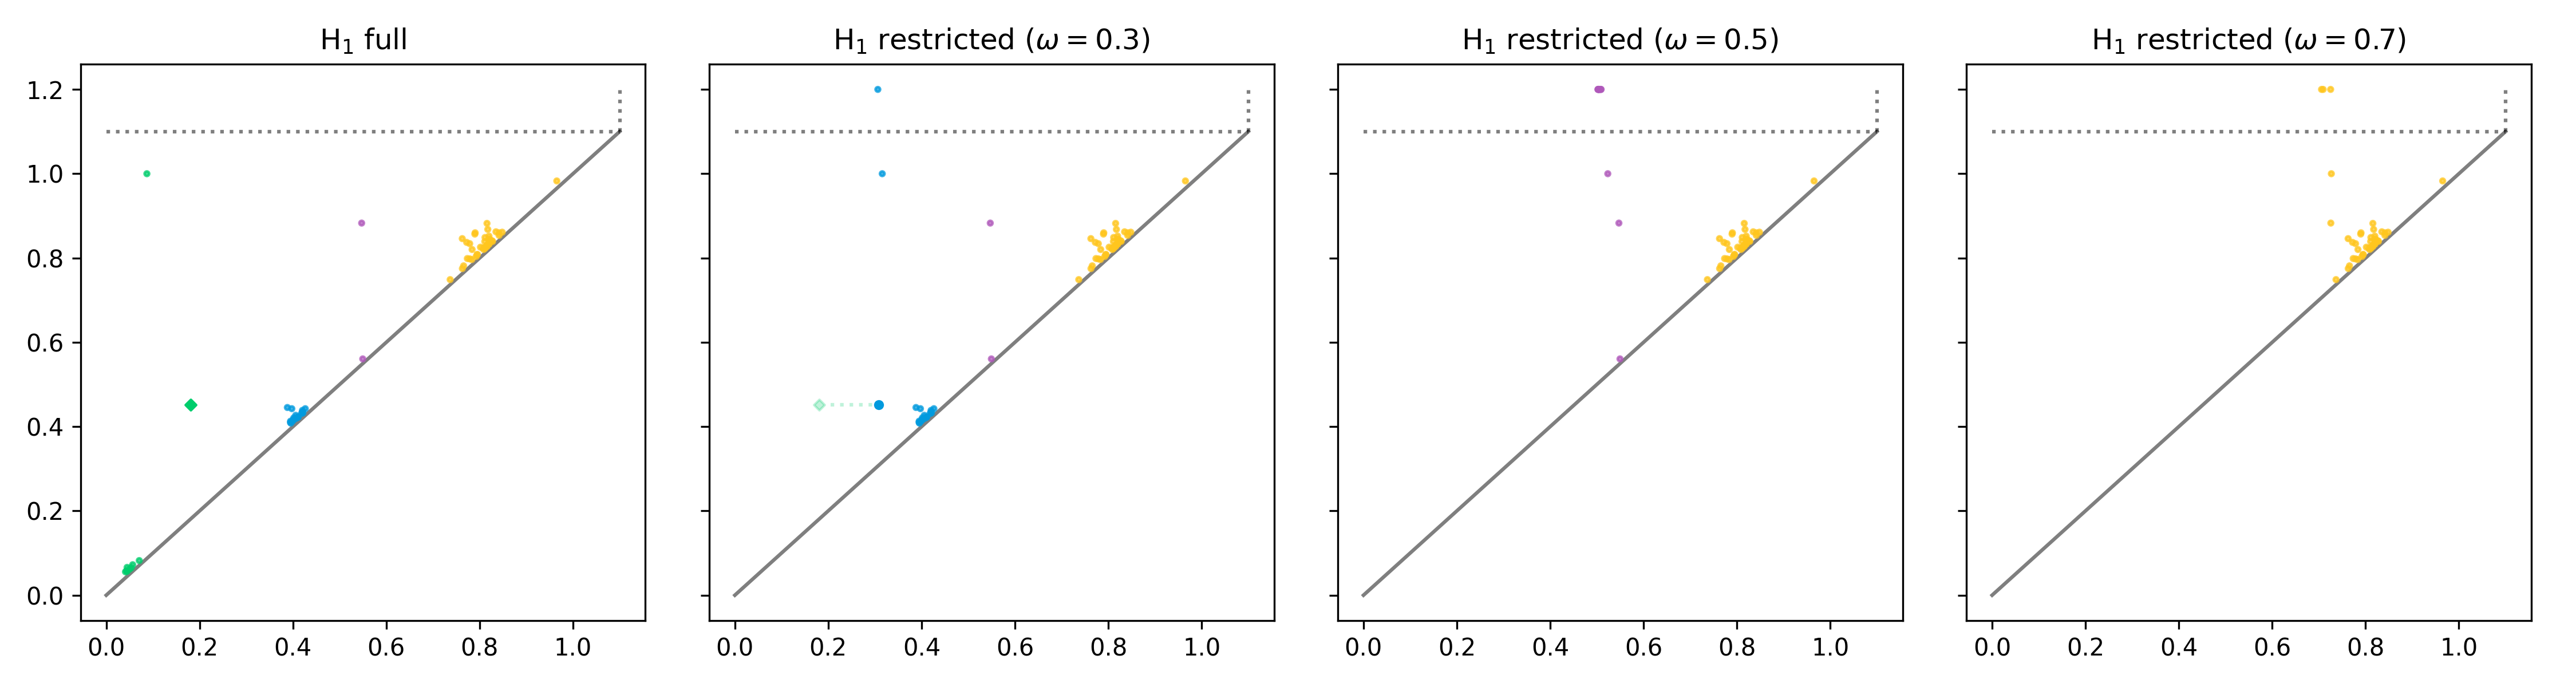
\includegraphics[trim=0 0 525 0, clip, width=0.7\textwidth]{scripts/figures/matching2/dgm-0.png}\\
  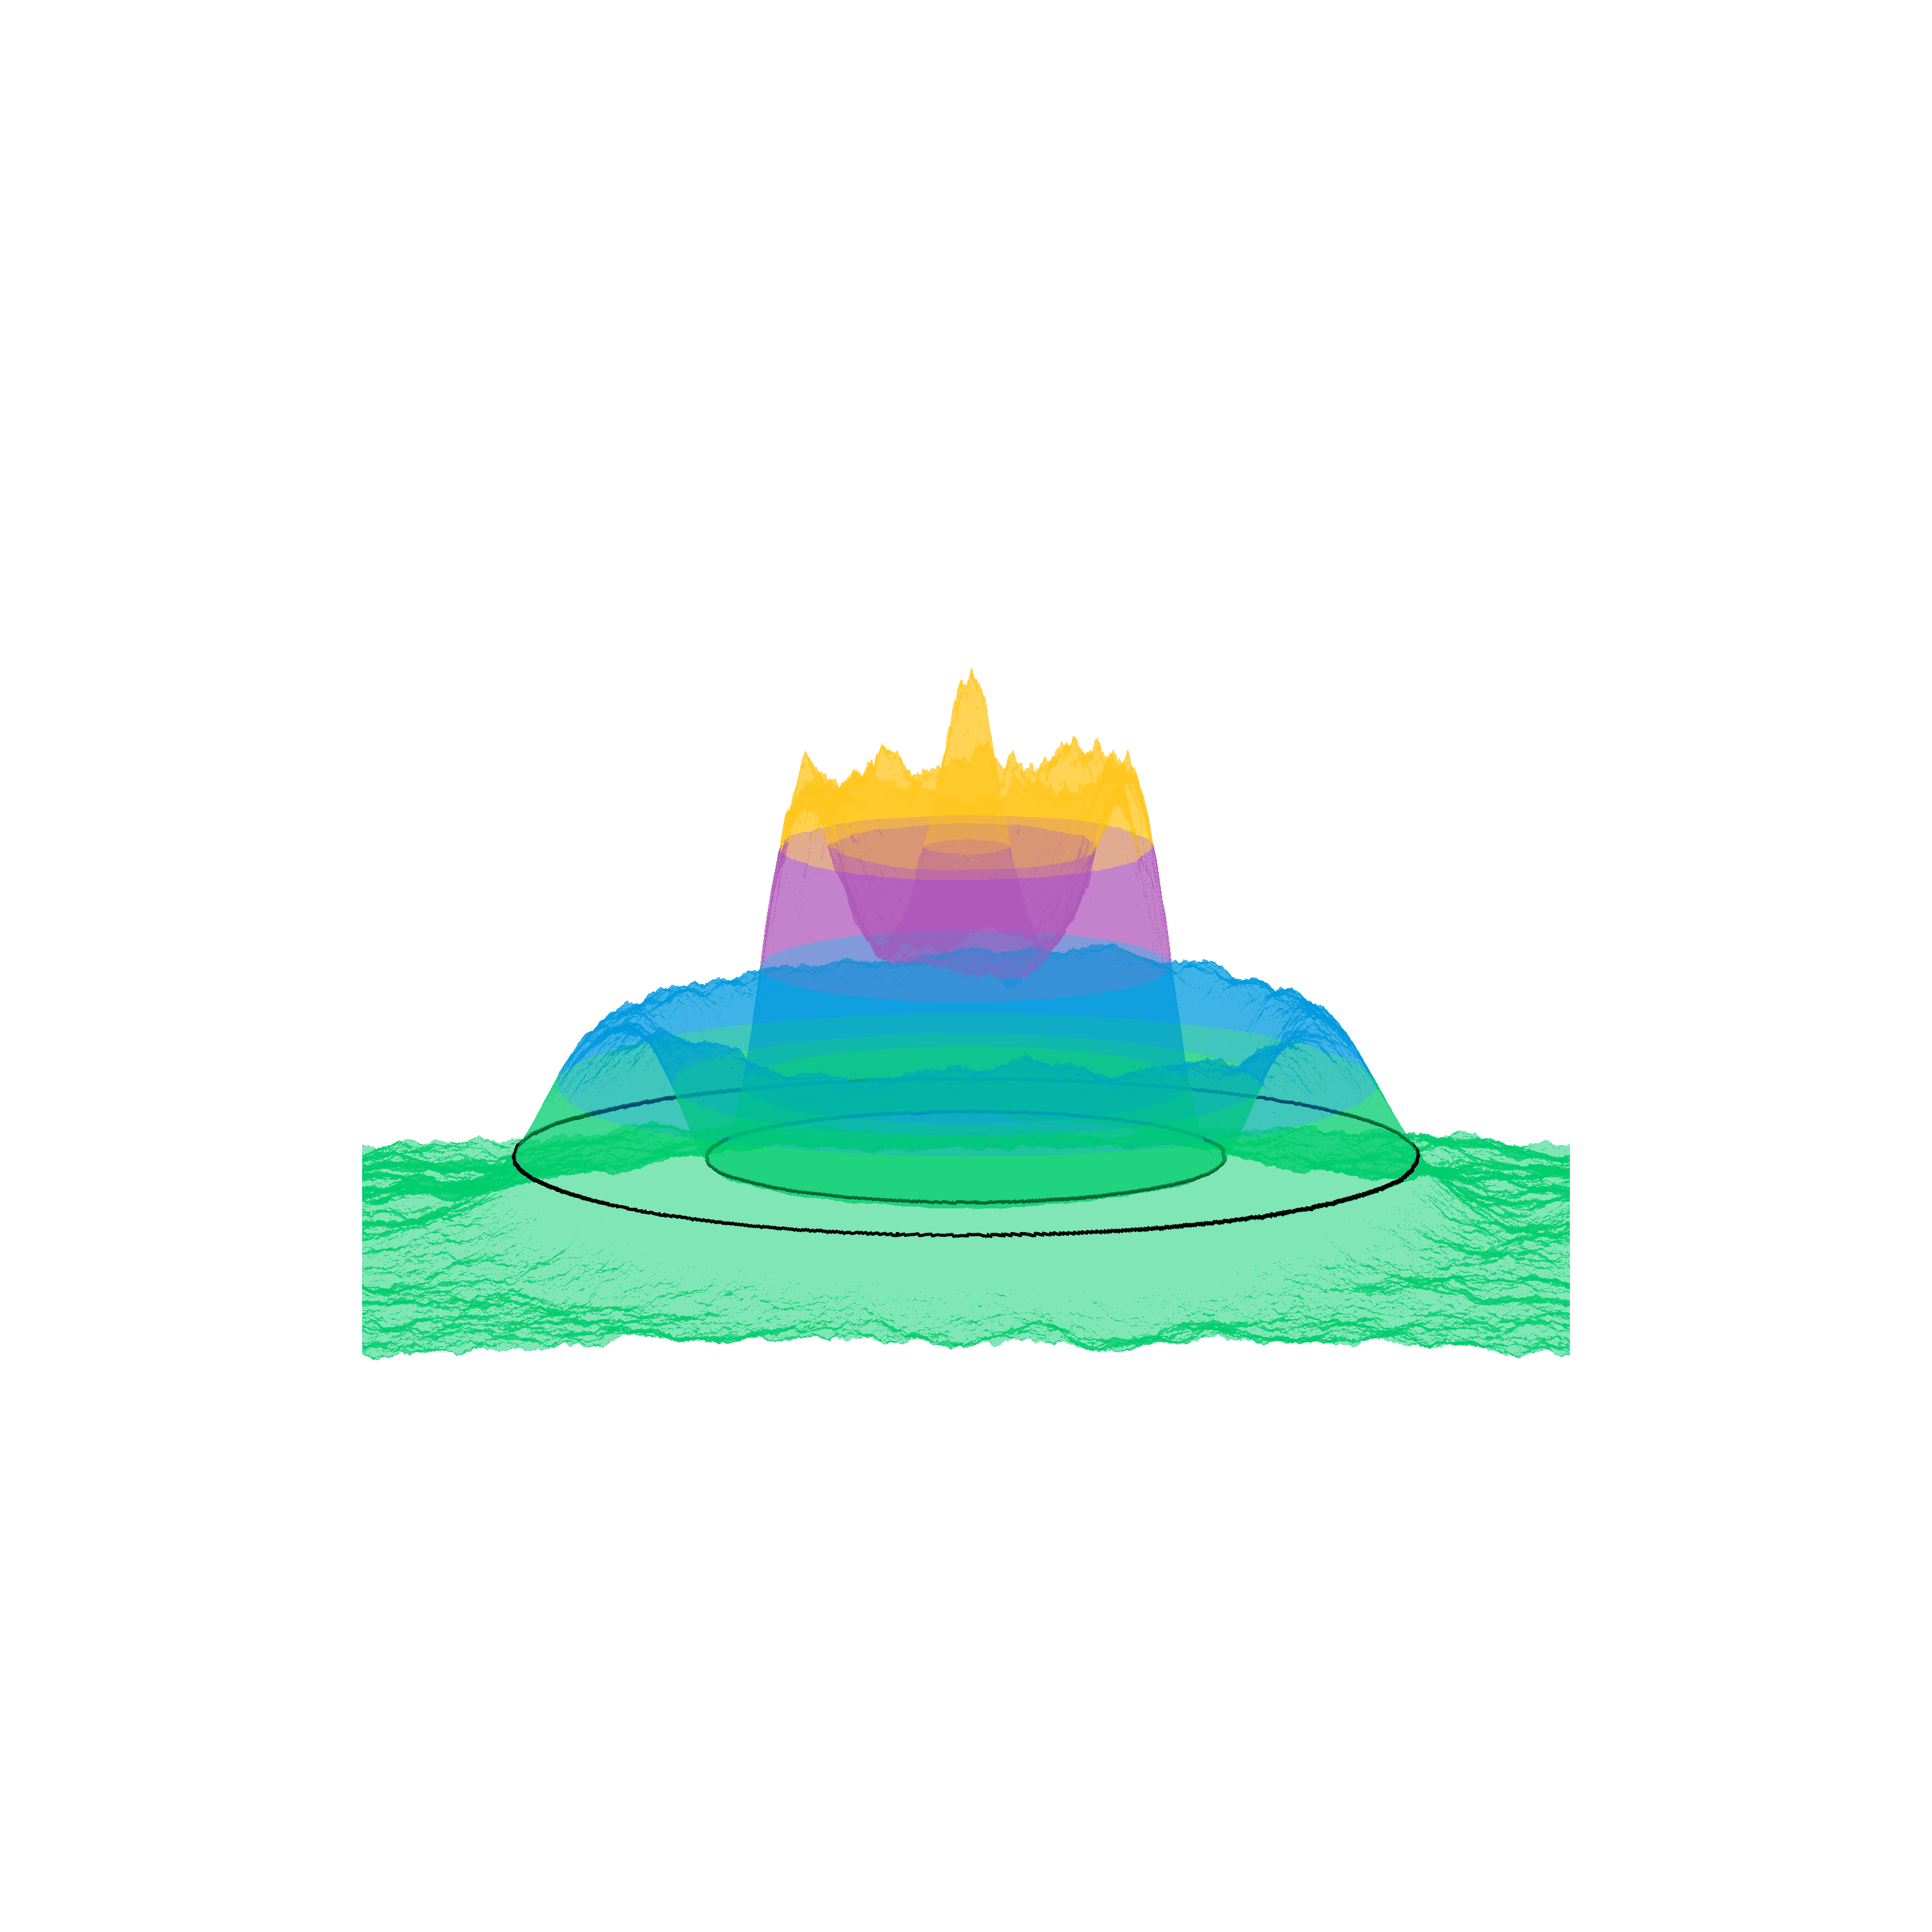
\includegraphics[trim=500 800 500 800, clip, width=0.3\textwidth]{scripts/figures/matching2/surf_side-0.png}
  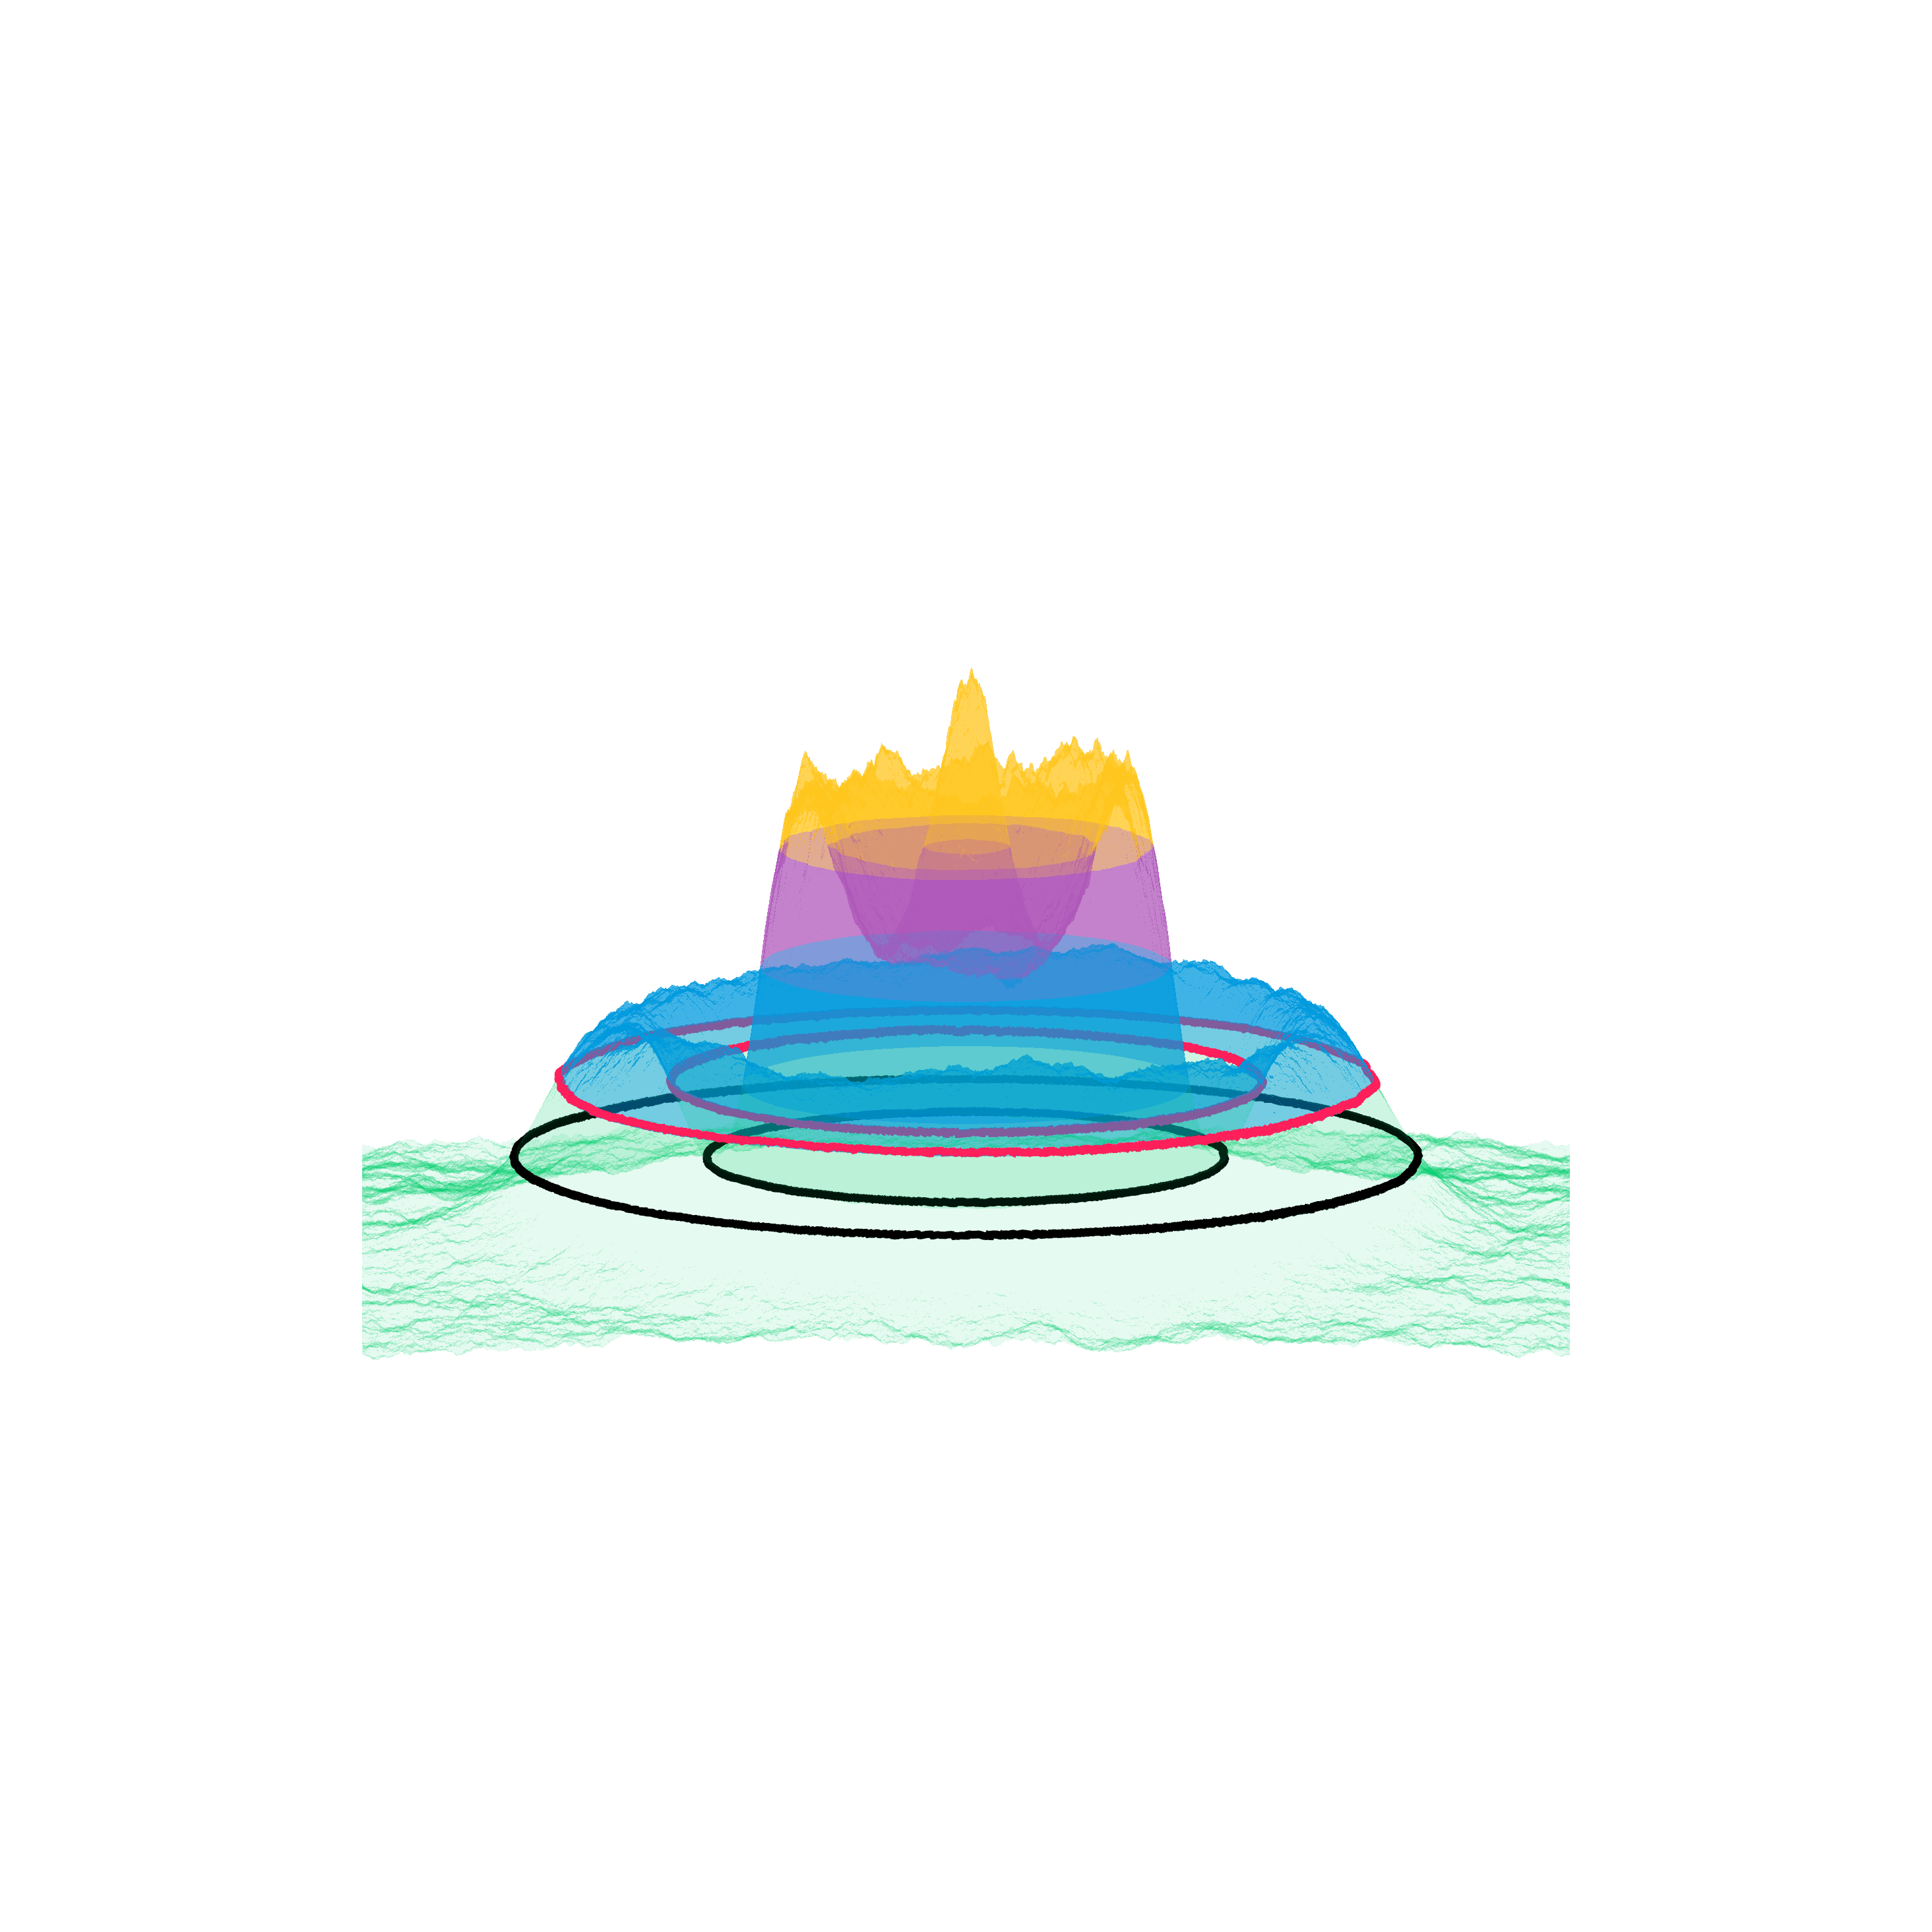
\includegraphics[trim=500 800 500 800, clip, width=0.3\textwidth]{scripts/figures/matching2/surf_side-0_0.png}\\
  % 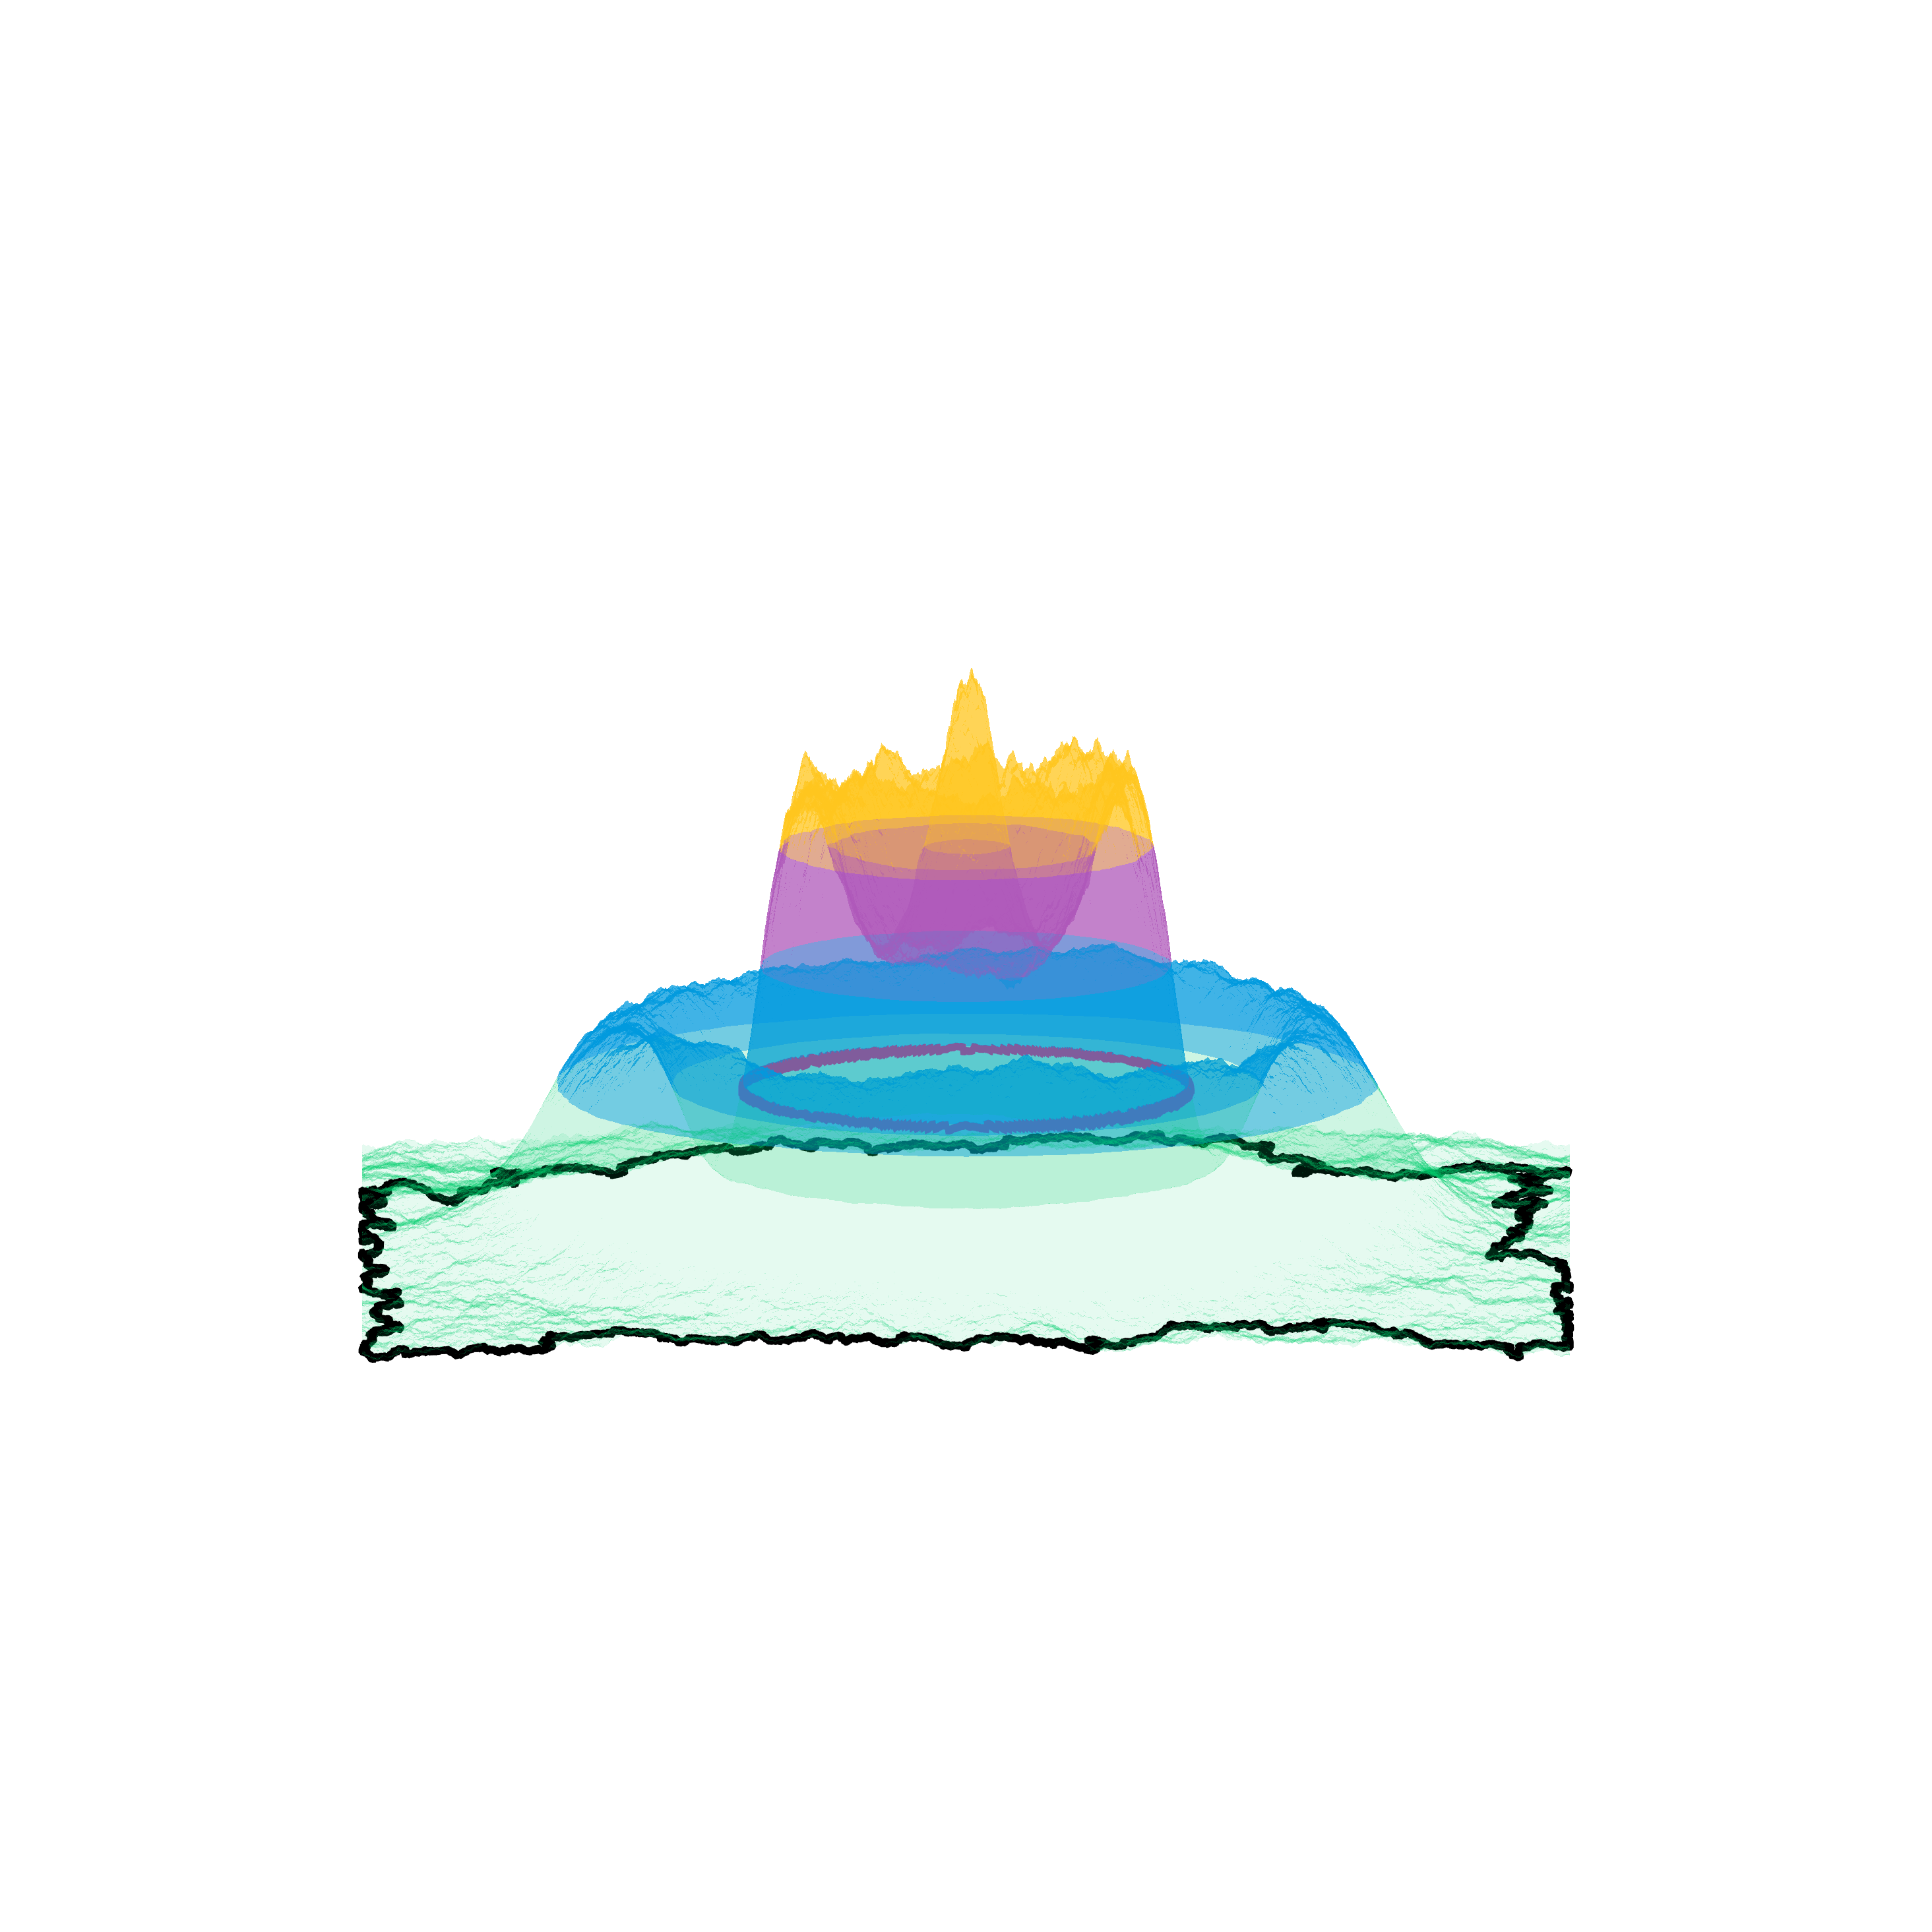
\includegraphics[trim=500 800 500 800, clip, width=0.24\textwidth]{scripts/figures/matching2/surf_side-0_1.png}
  % \includegraphics[trim=500 800 500 800, clip, width=0.24\textwidth]{scripts/figures/matching2/surf_side-0_2.png}
  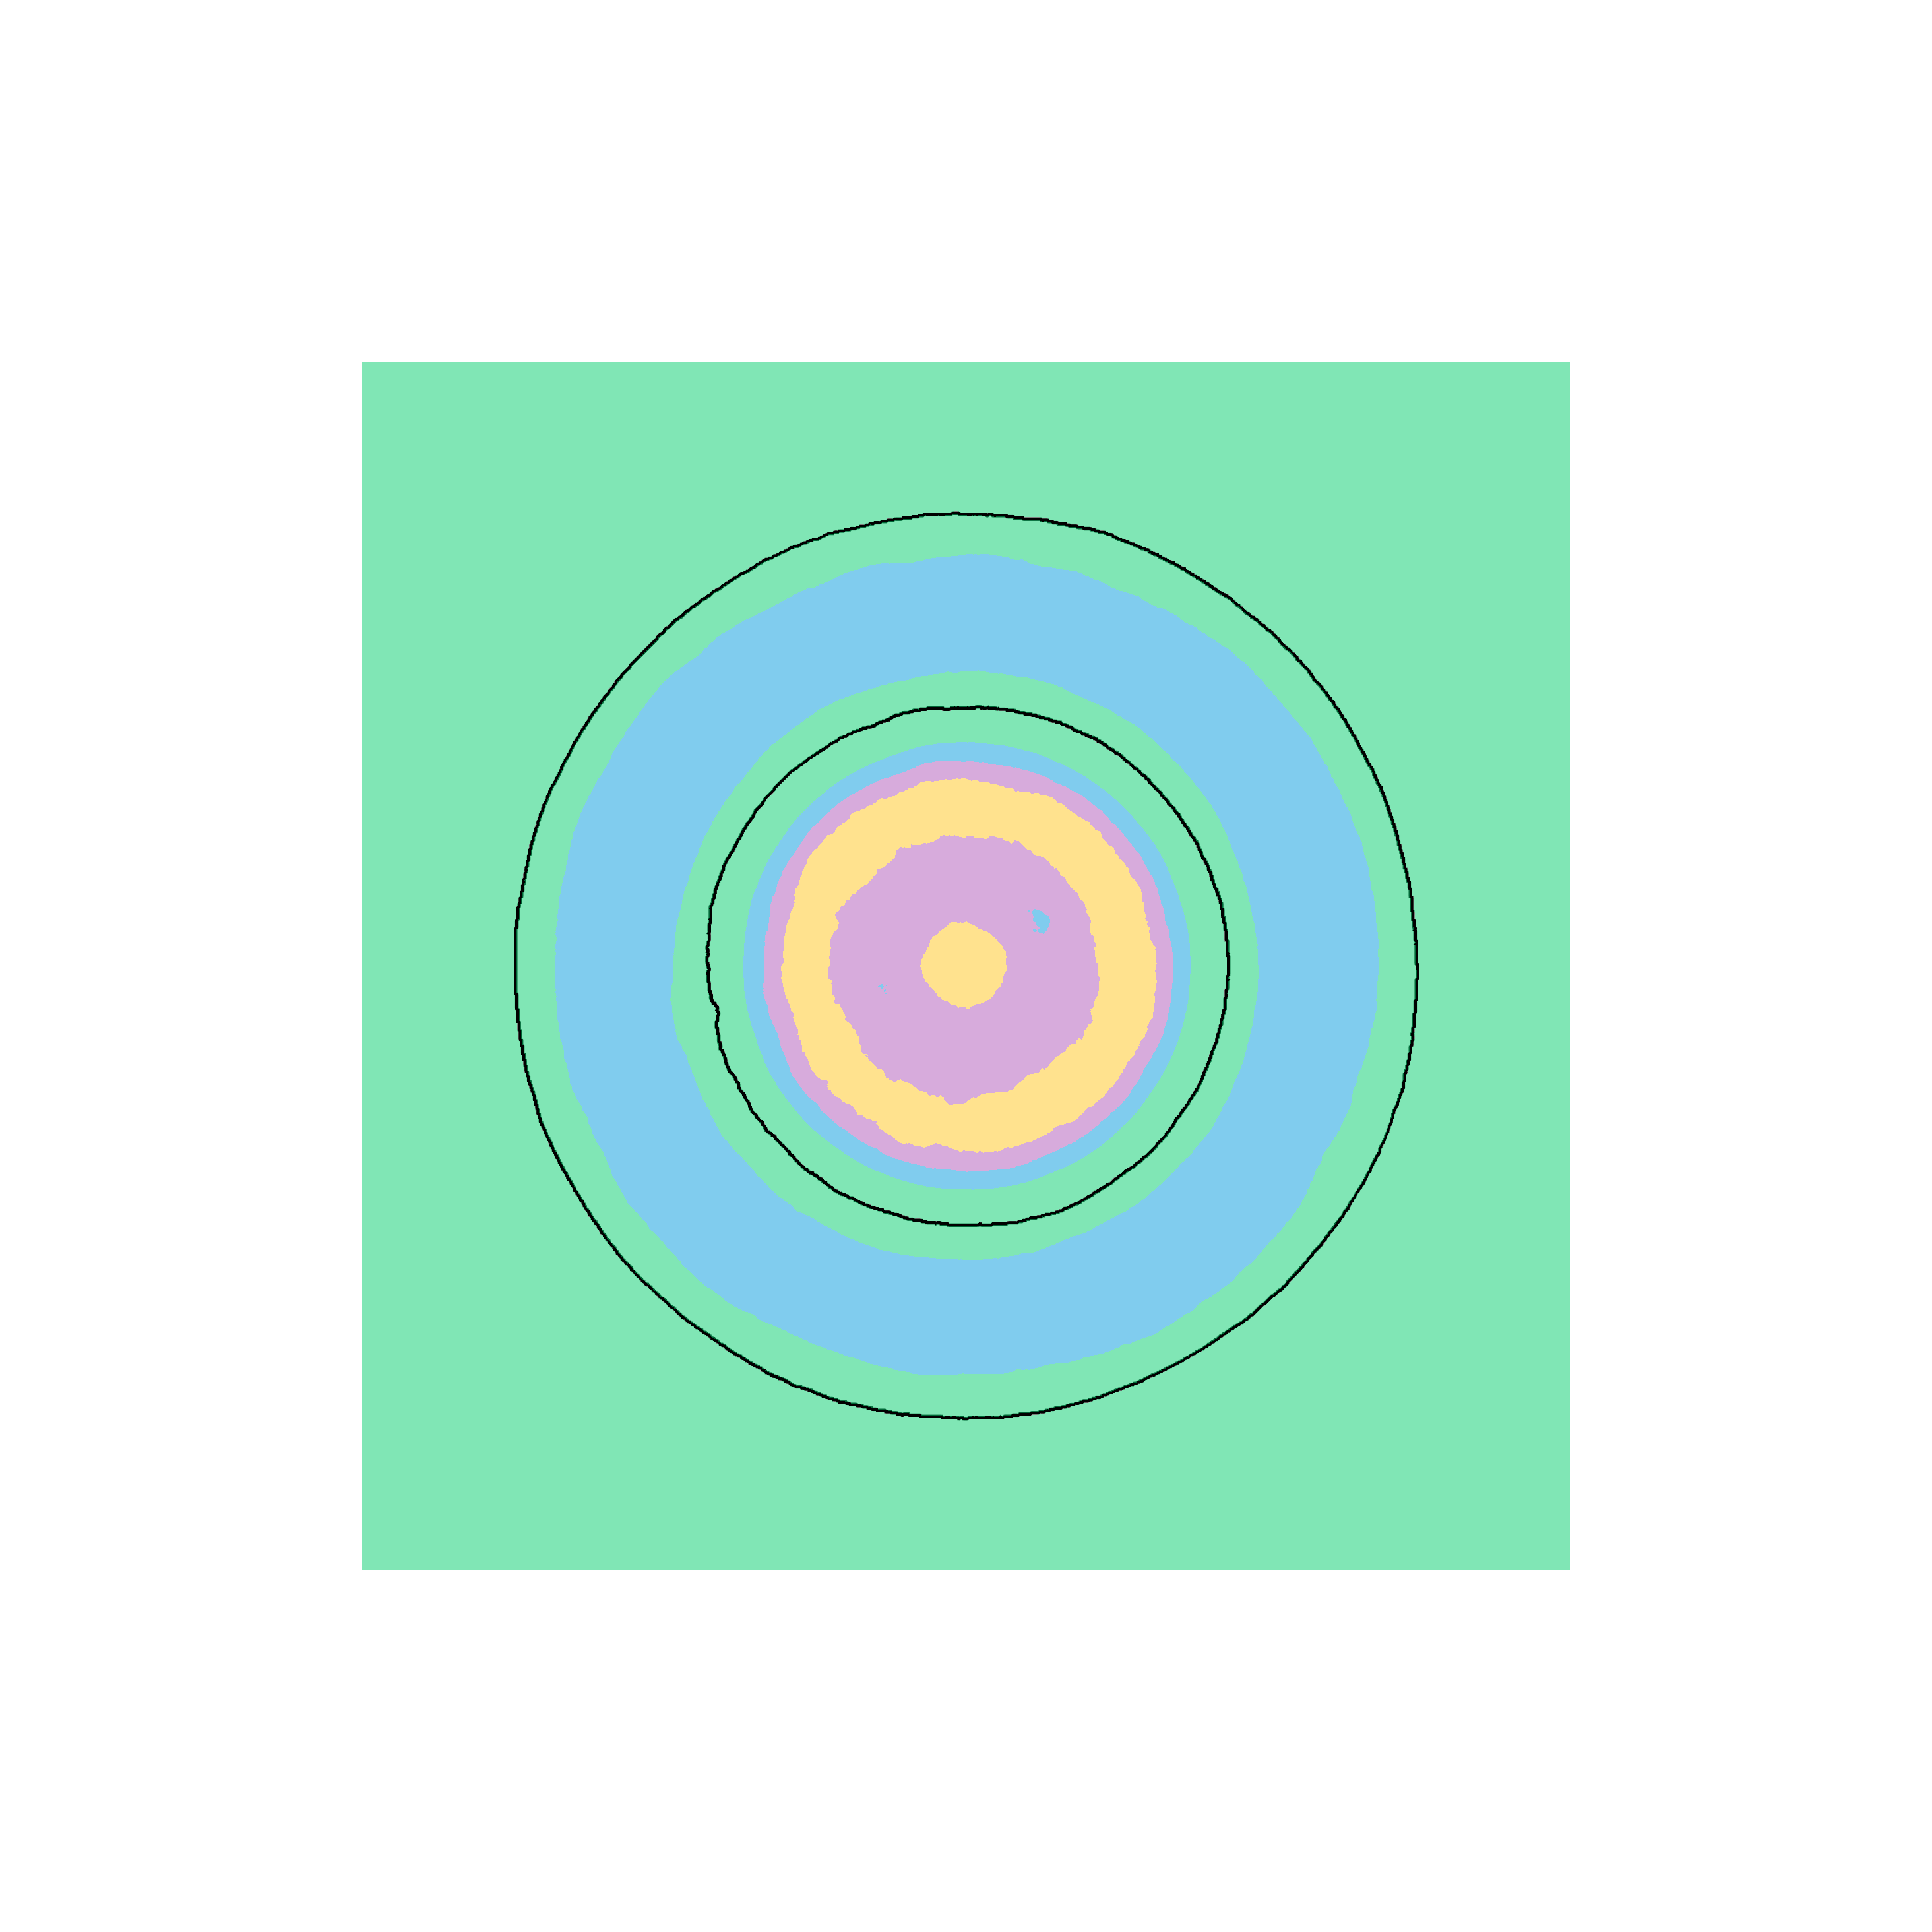
\includegraphics[trim=500 500 500 500, clip, width=0.3\textwidth]{scripts/figures/matching2/surf_top-0.png}
  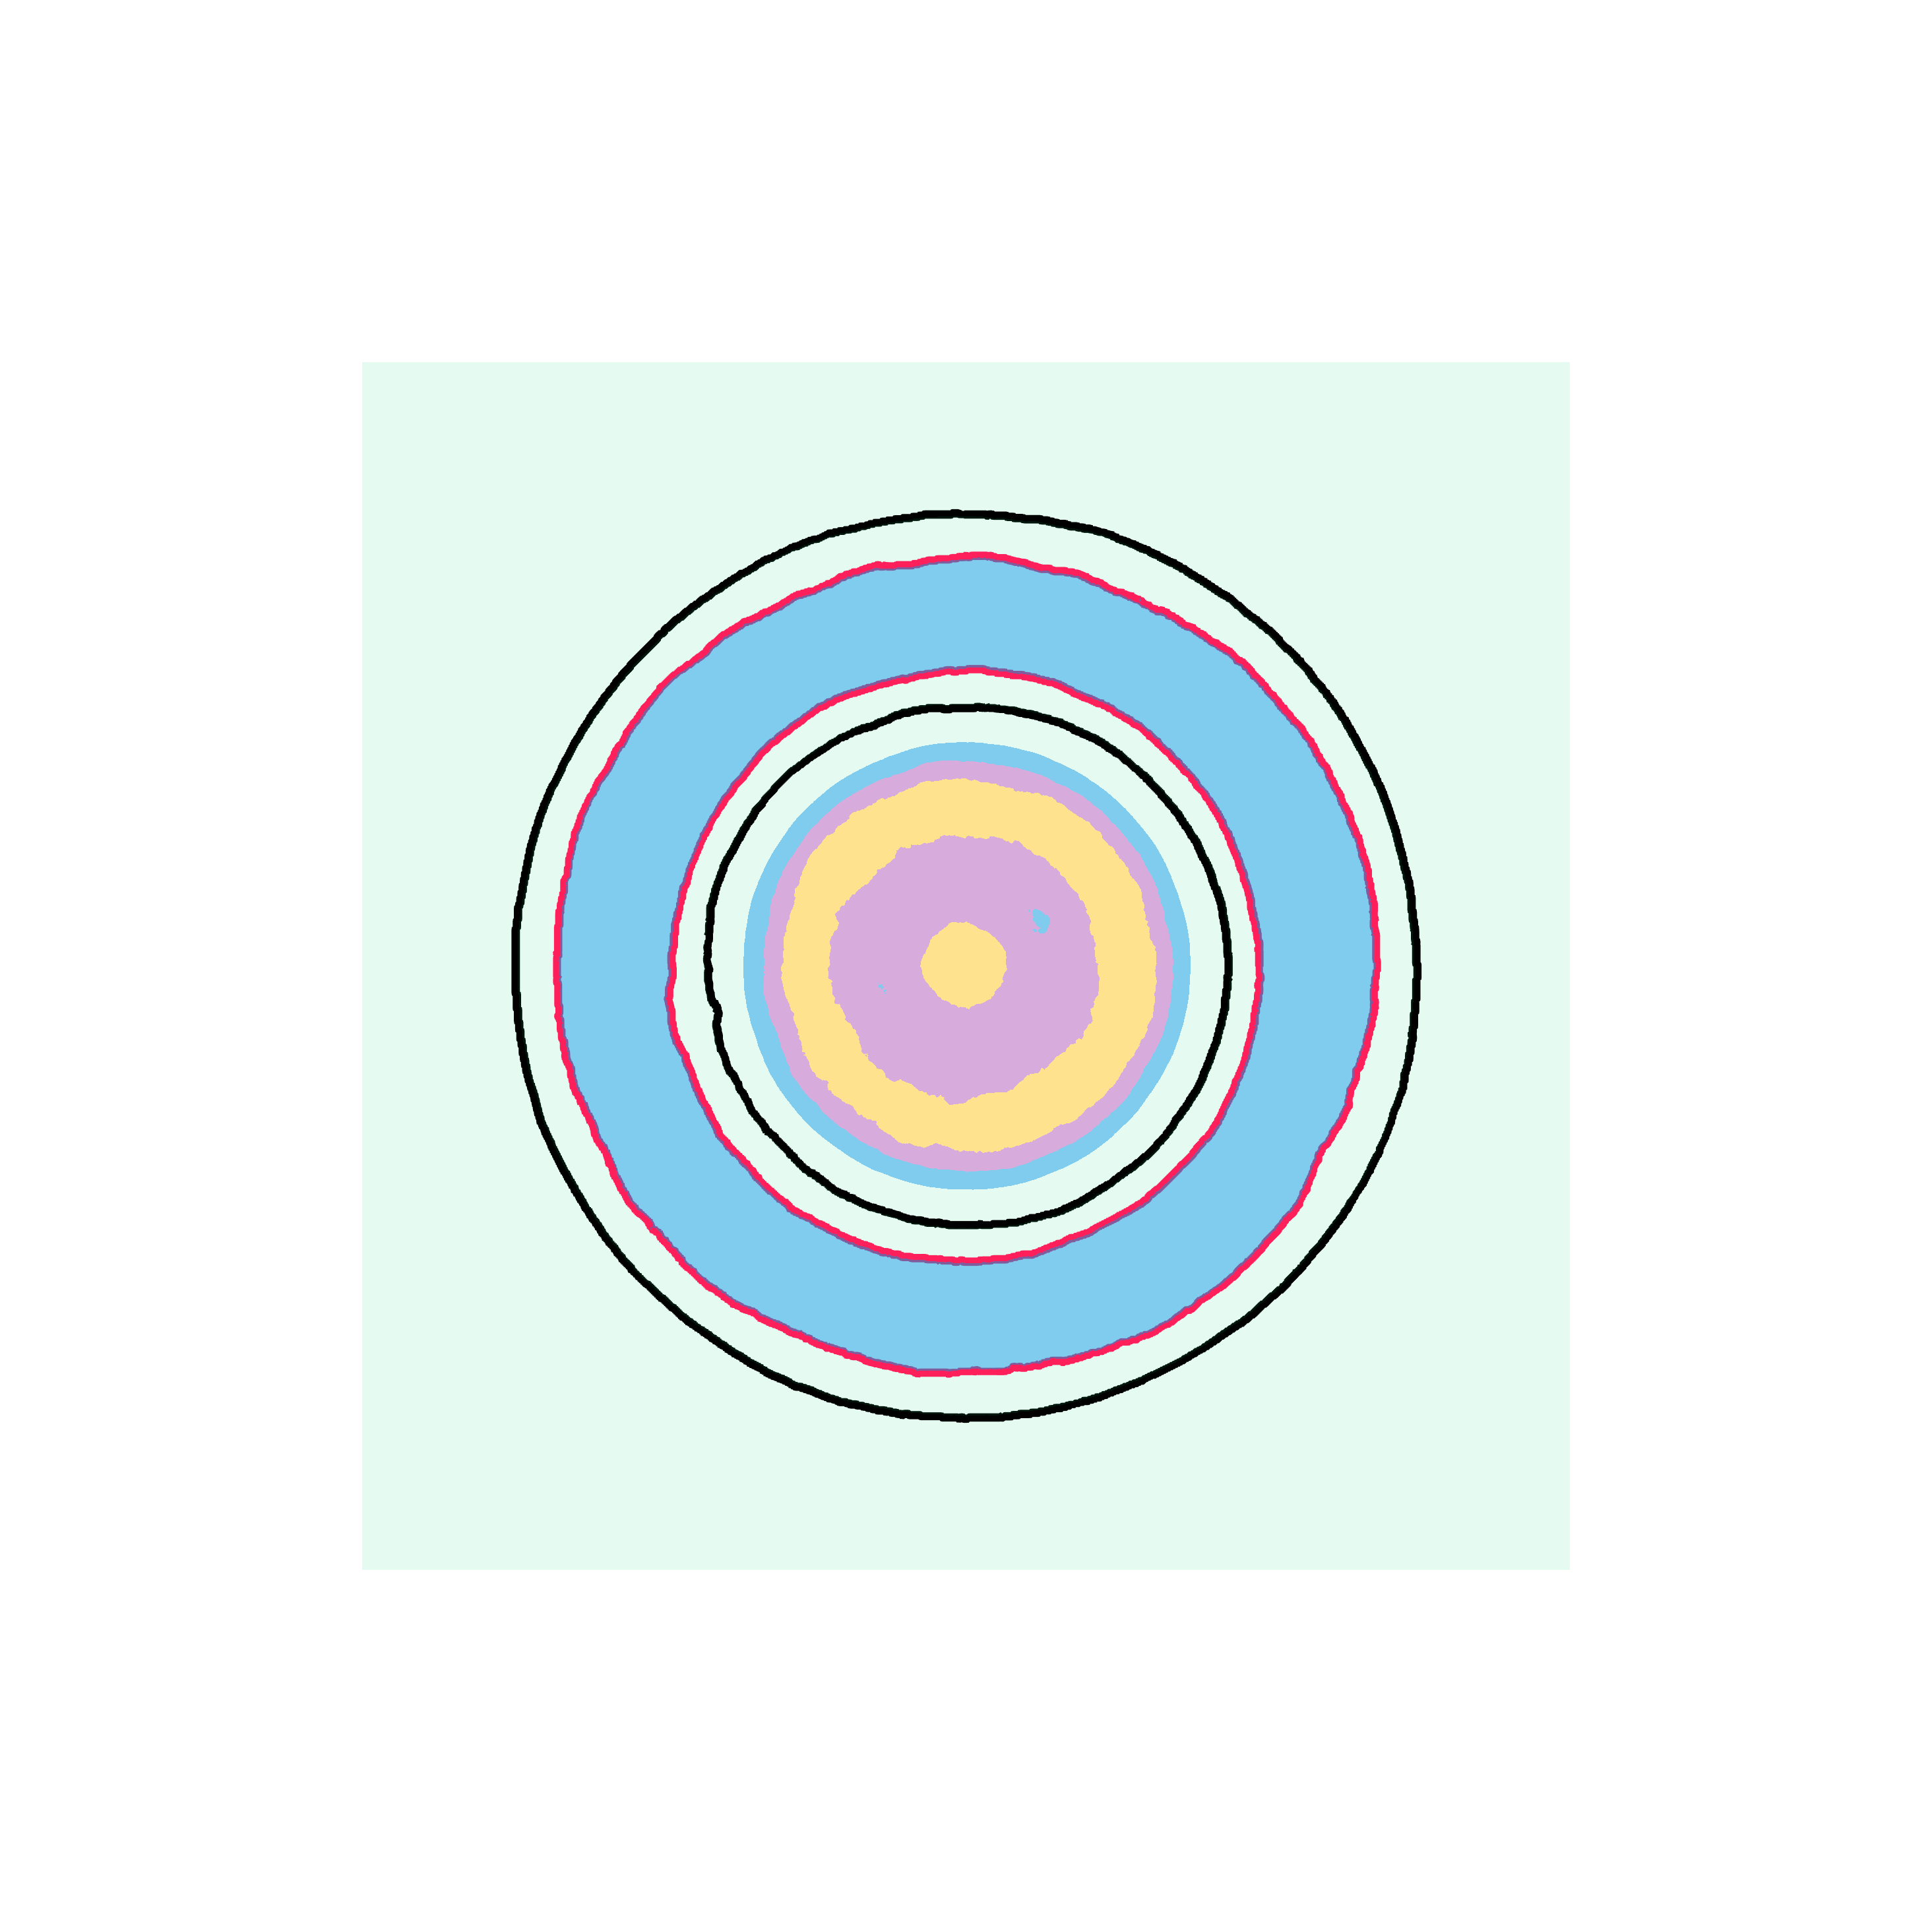
\includegraphics[trim=500 500 500 500, clip, width=0.3\textwidth]{scripts/figures/matching2/surf_top-0_0.png}
  % 
\includegraphics[trim=500 500 500 500, clip, width=0.24\textwidth]{scripts/figures/matching2/surf_top-0_1.png}
  % \includegraphics[trim=500 500 500 500, clip, width=0.24\textwidth]{scripts/figures/matching2/surf_top-0_2.png}
\end{figure}

\begin{figure}[htbp]
  \centering
  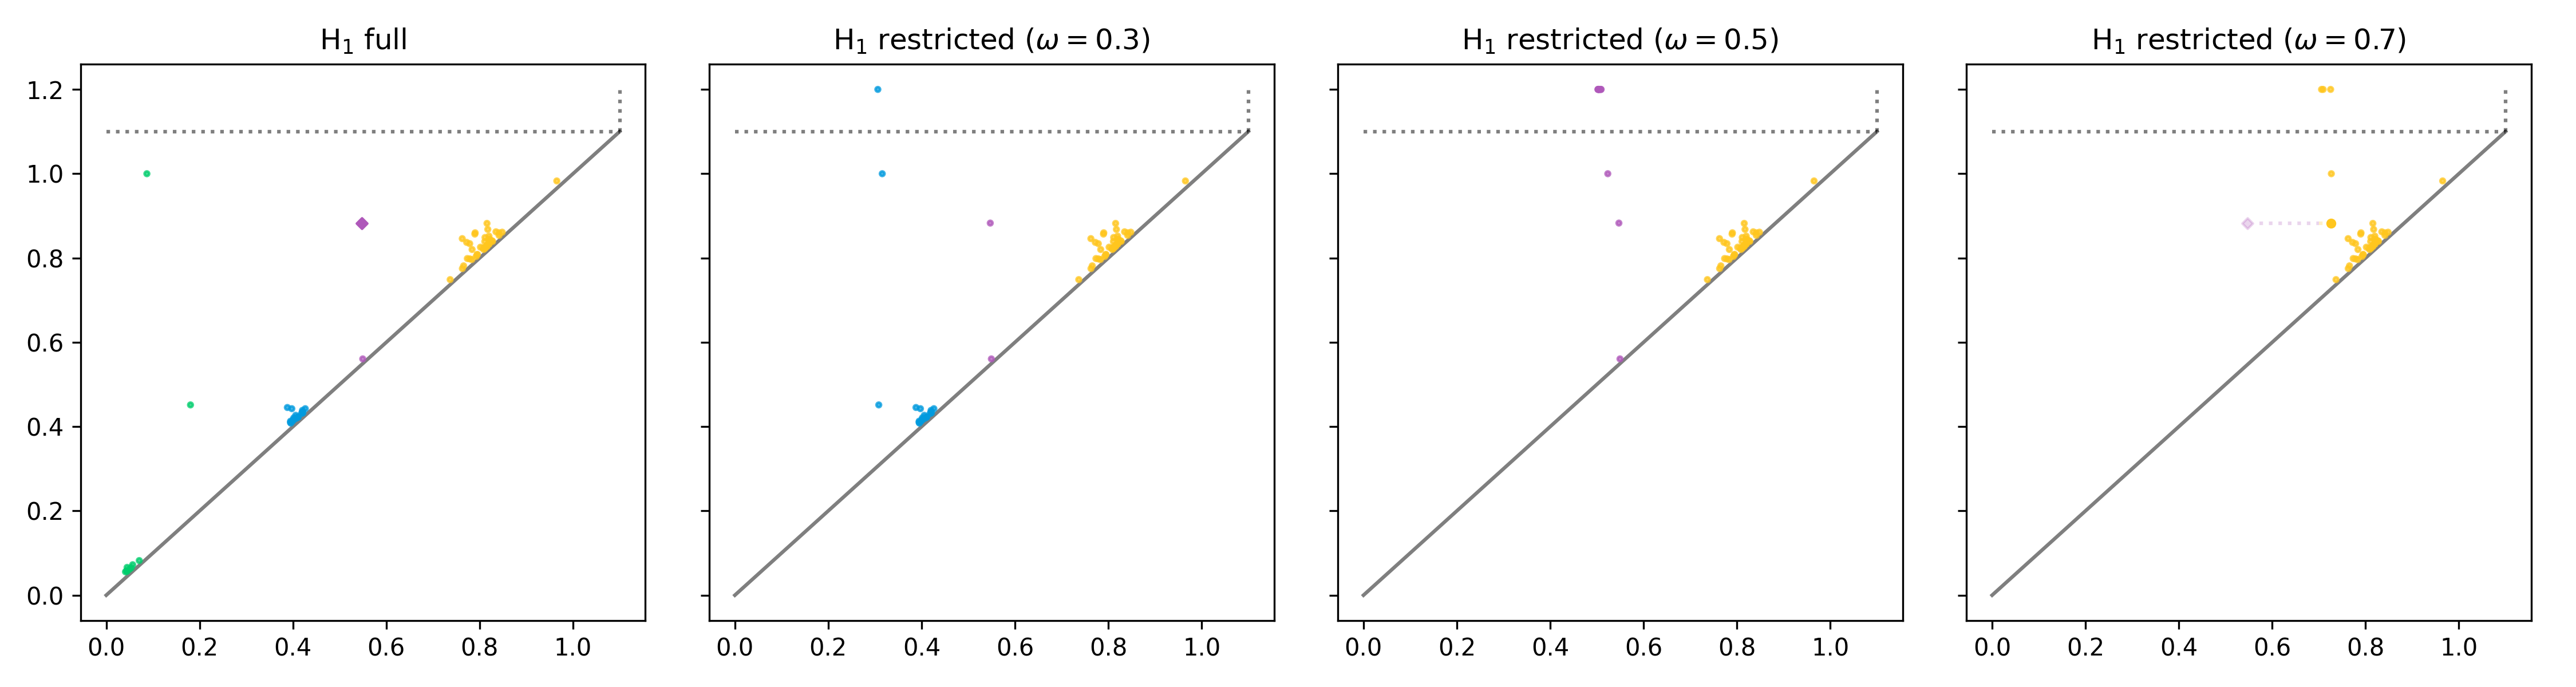
\includegraphics[trim=0 0 800 0, clip, width=0.35\textwidth]{scripts/figures/matching2/dgm-2.png}
  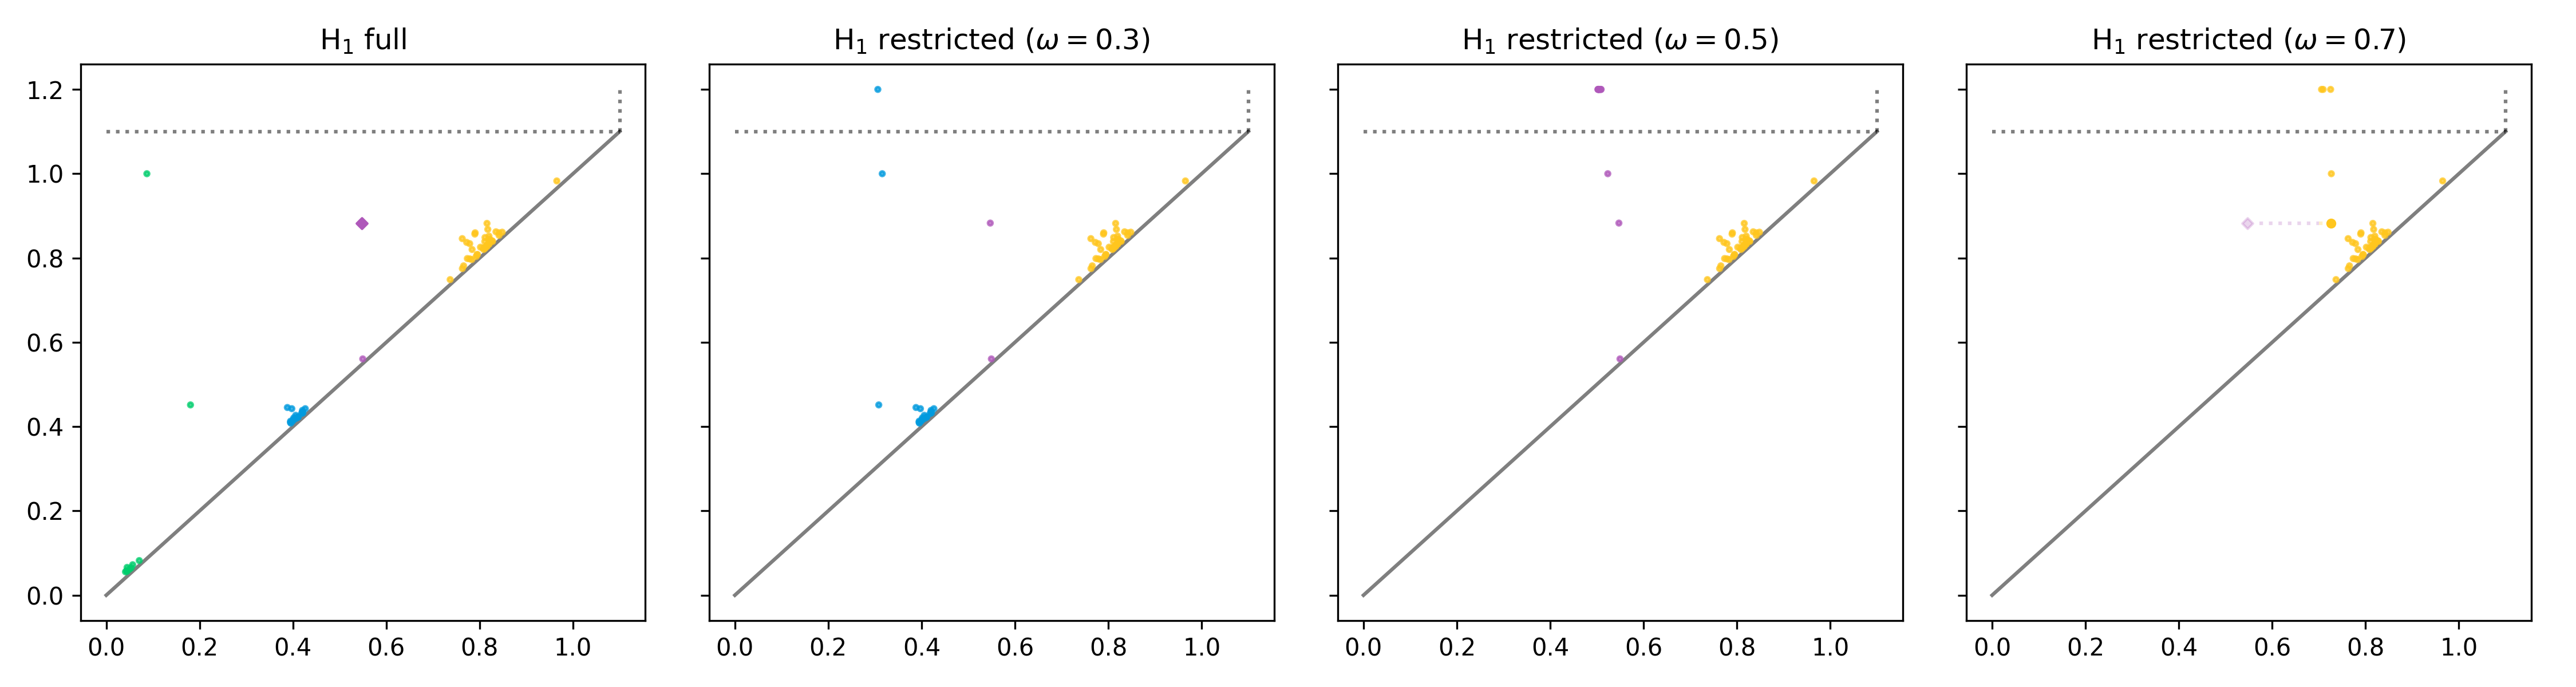
\includegraphics[trim=800 0 0 0, clip, width=0.35\textwidth]{scripts/figures/matching2/dgm-2.png}\\
  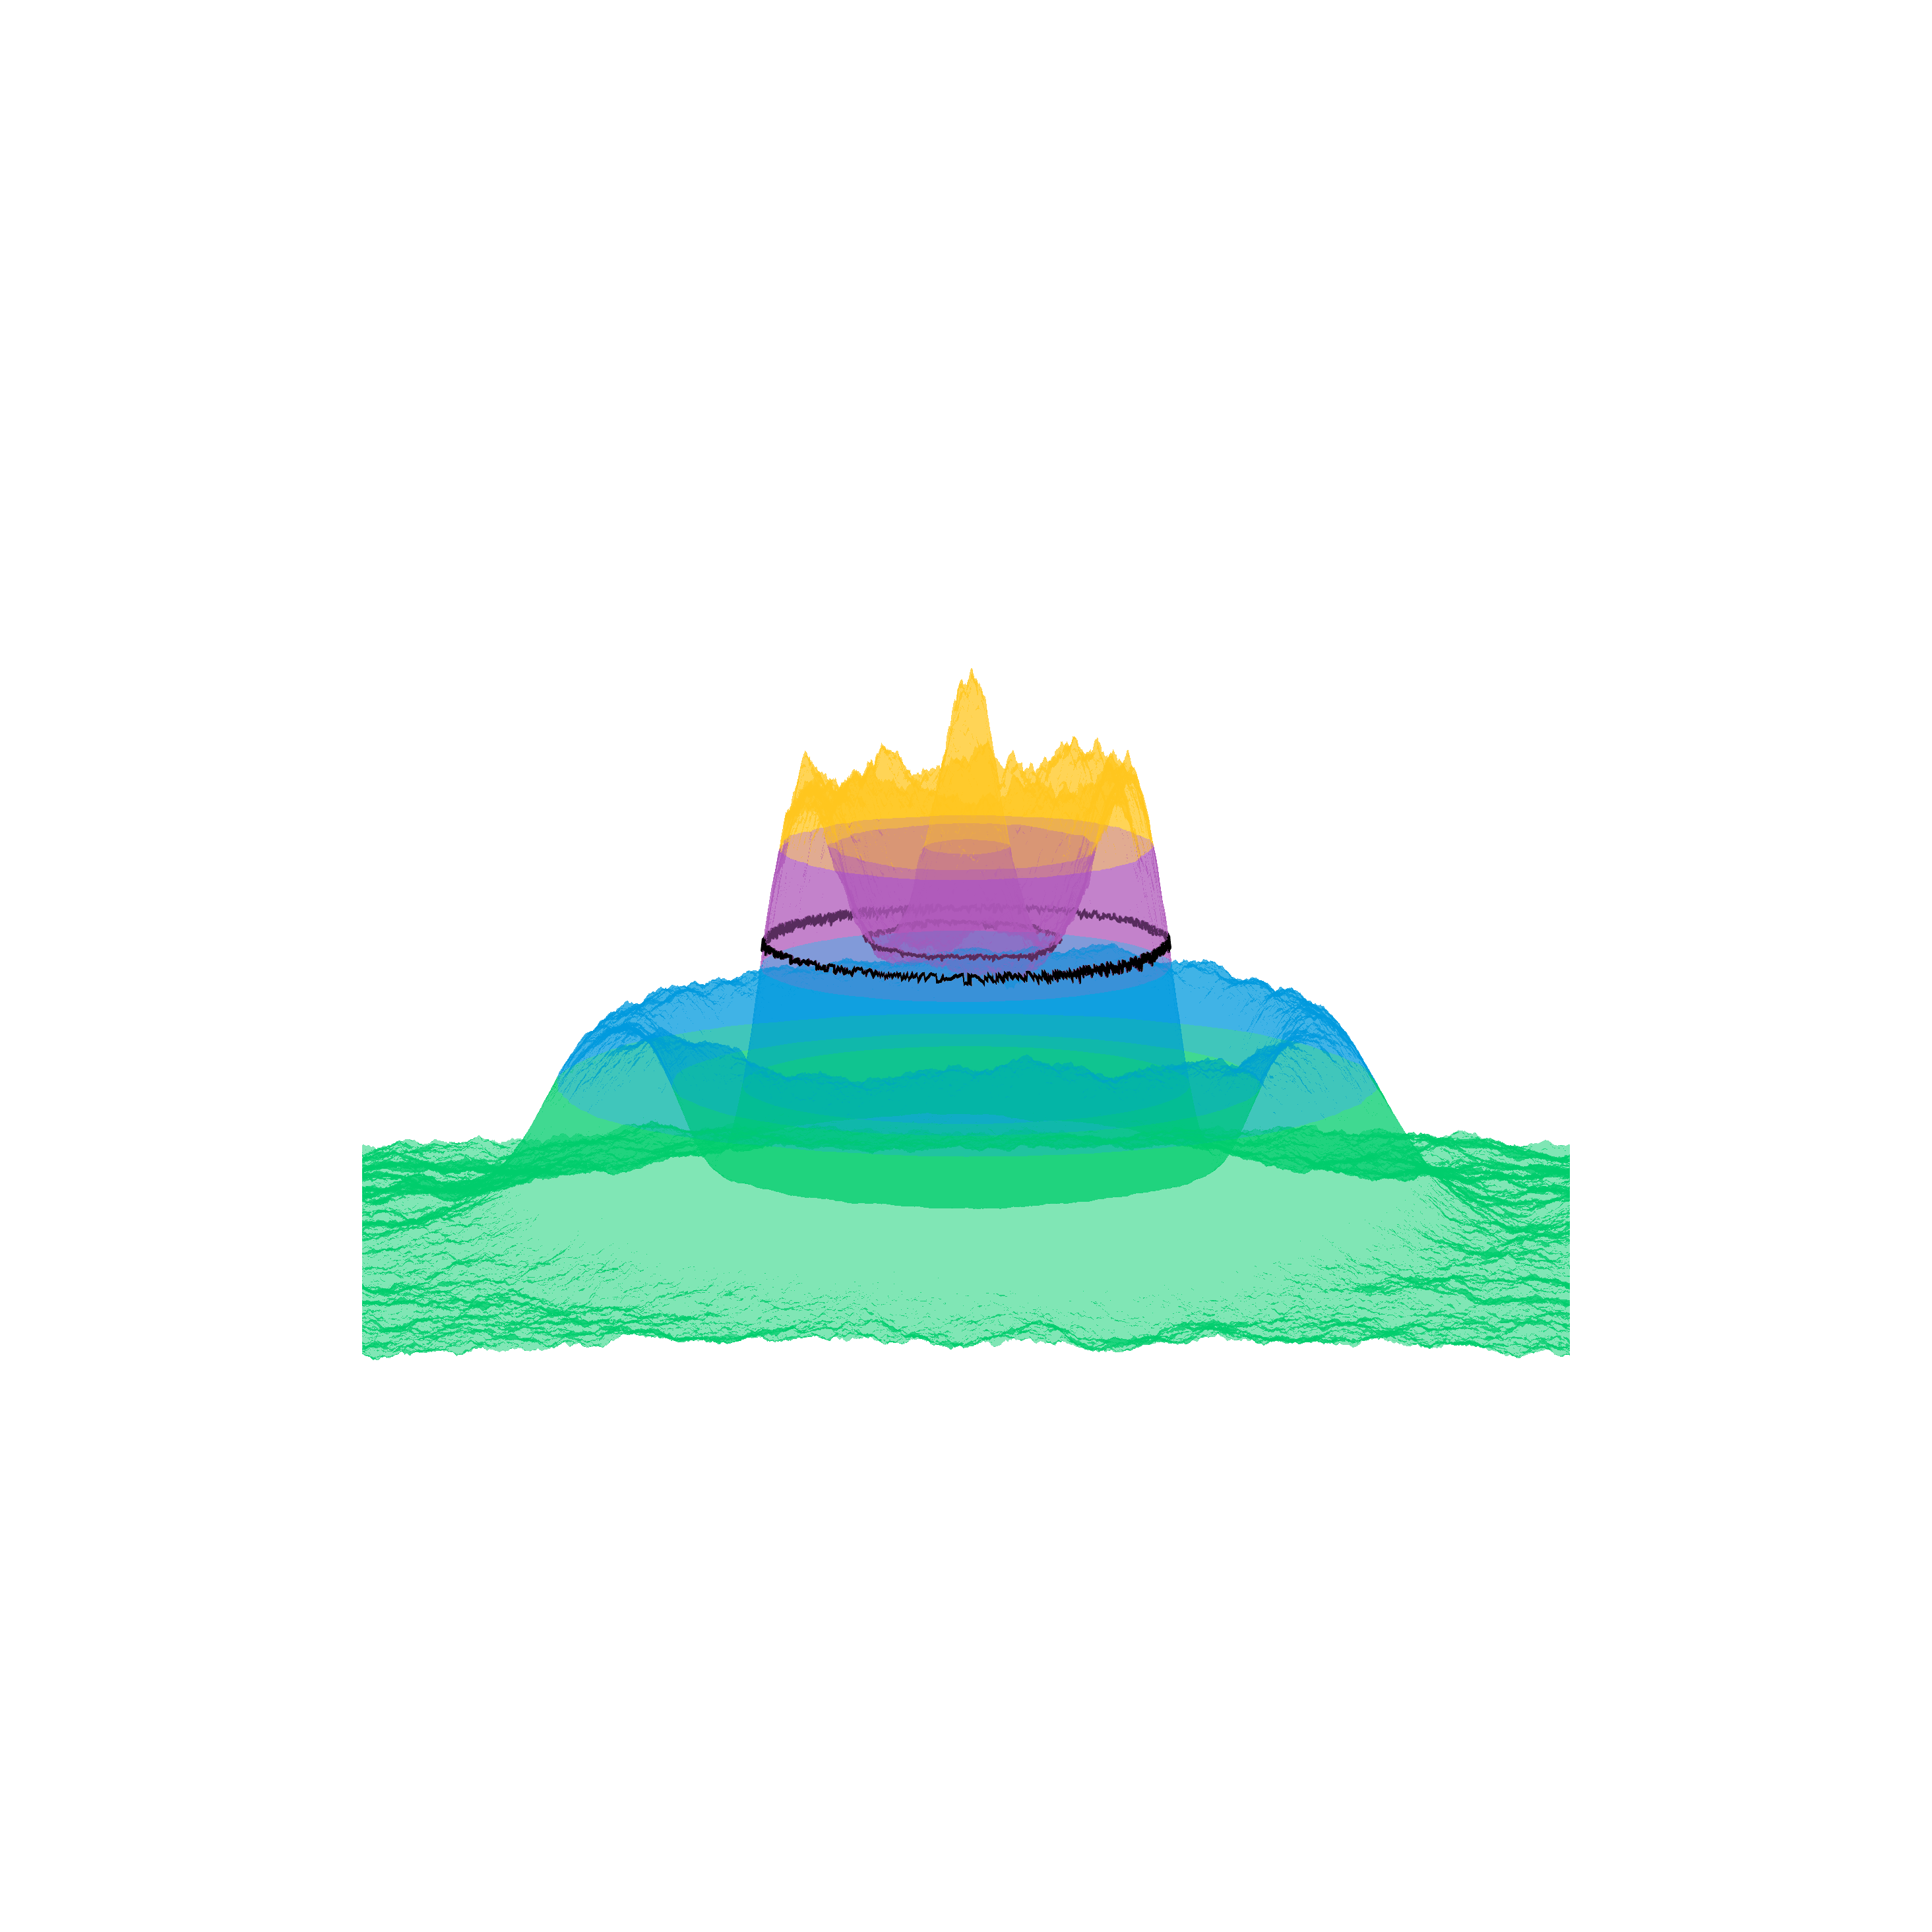
\includegraphics[trim=500 800 500 800, clip, width=0.3\textwidth]{scripts/figures/matching2/surf_side-2.png}
  % 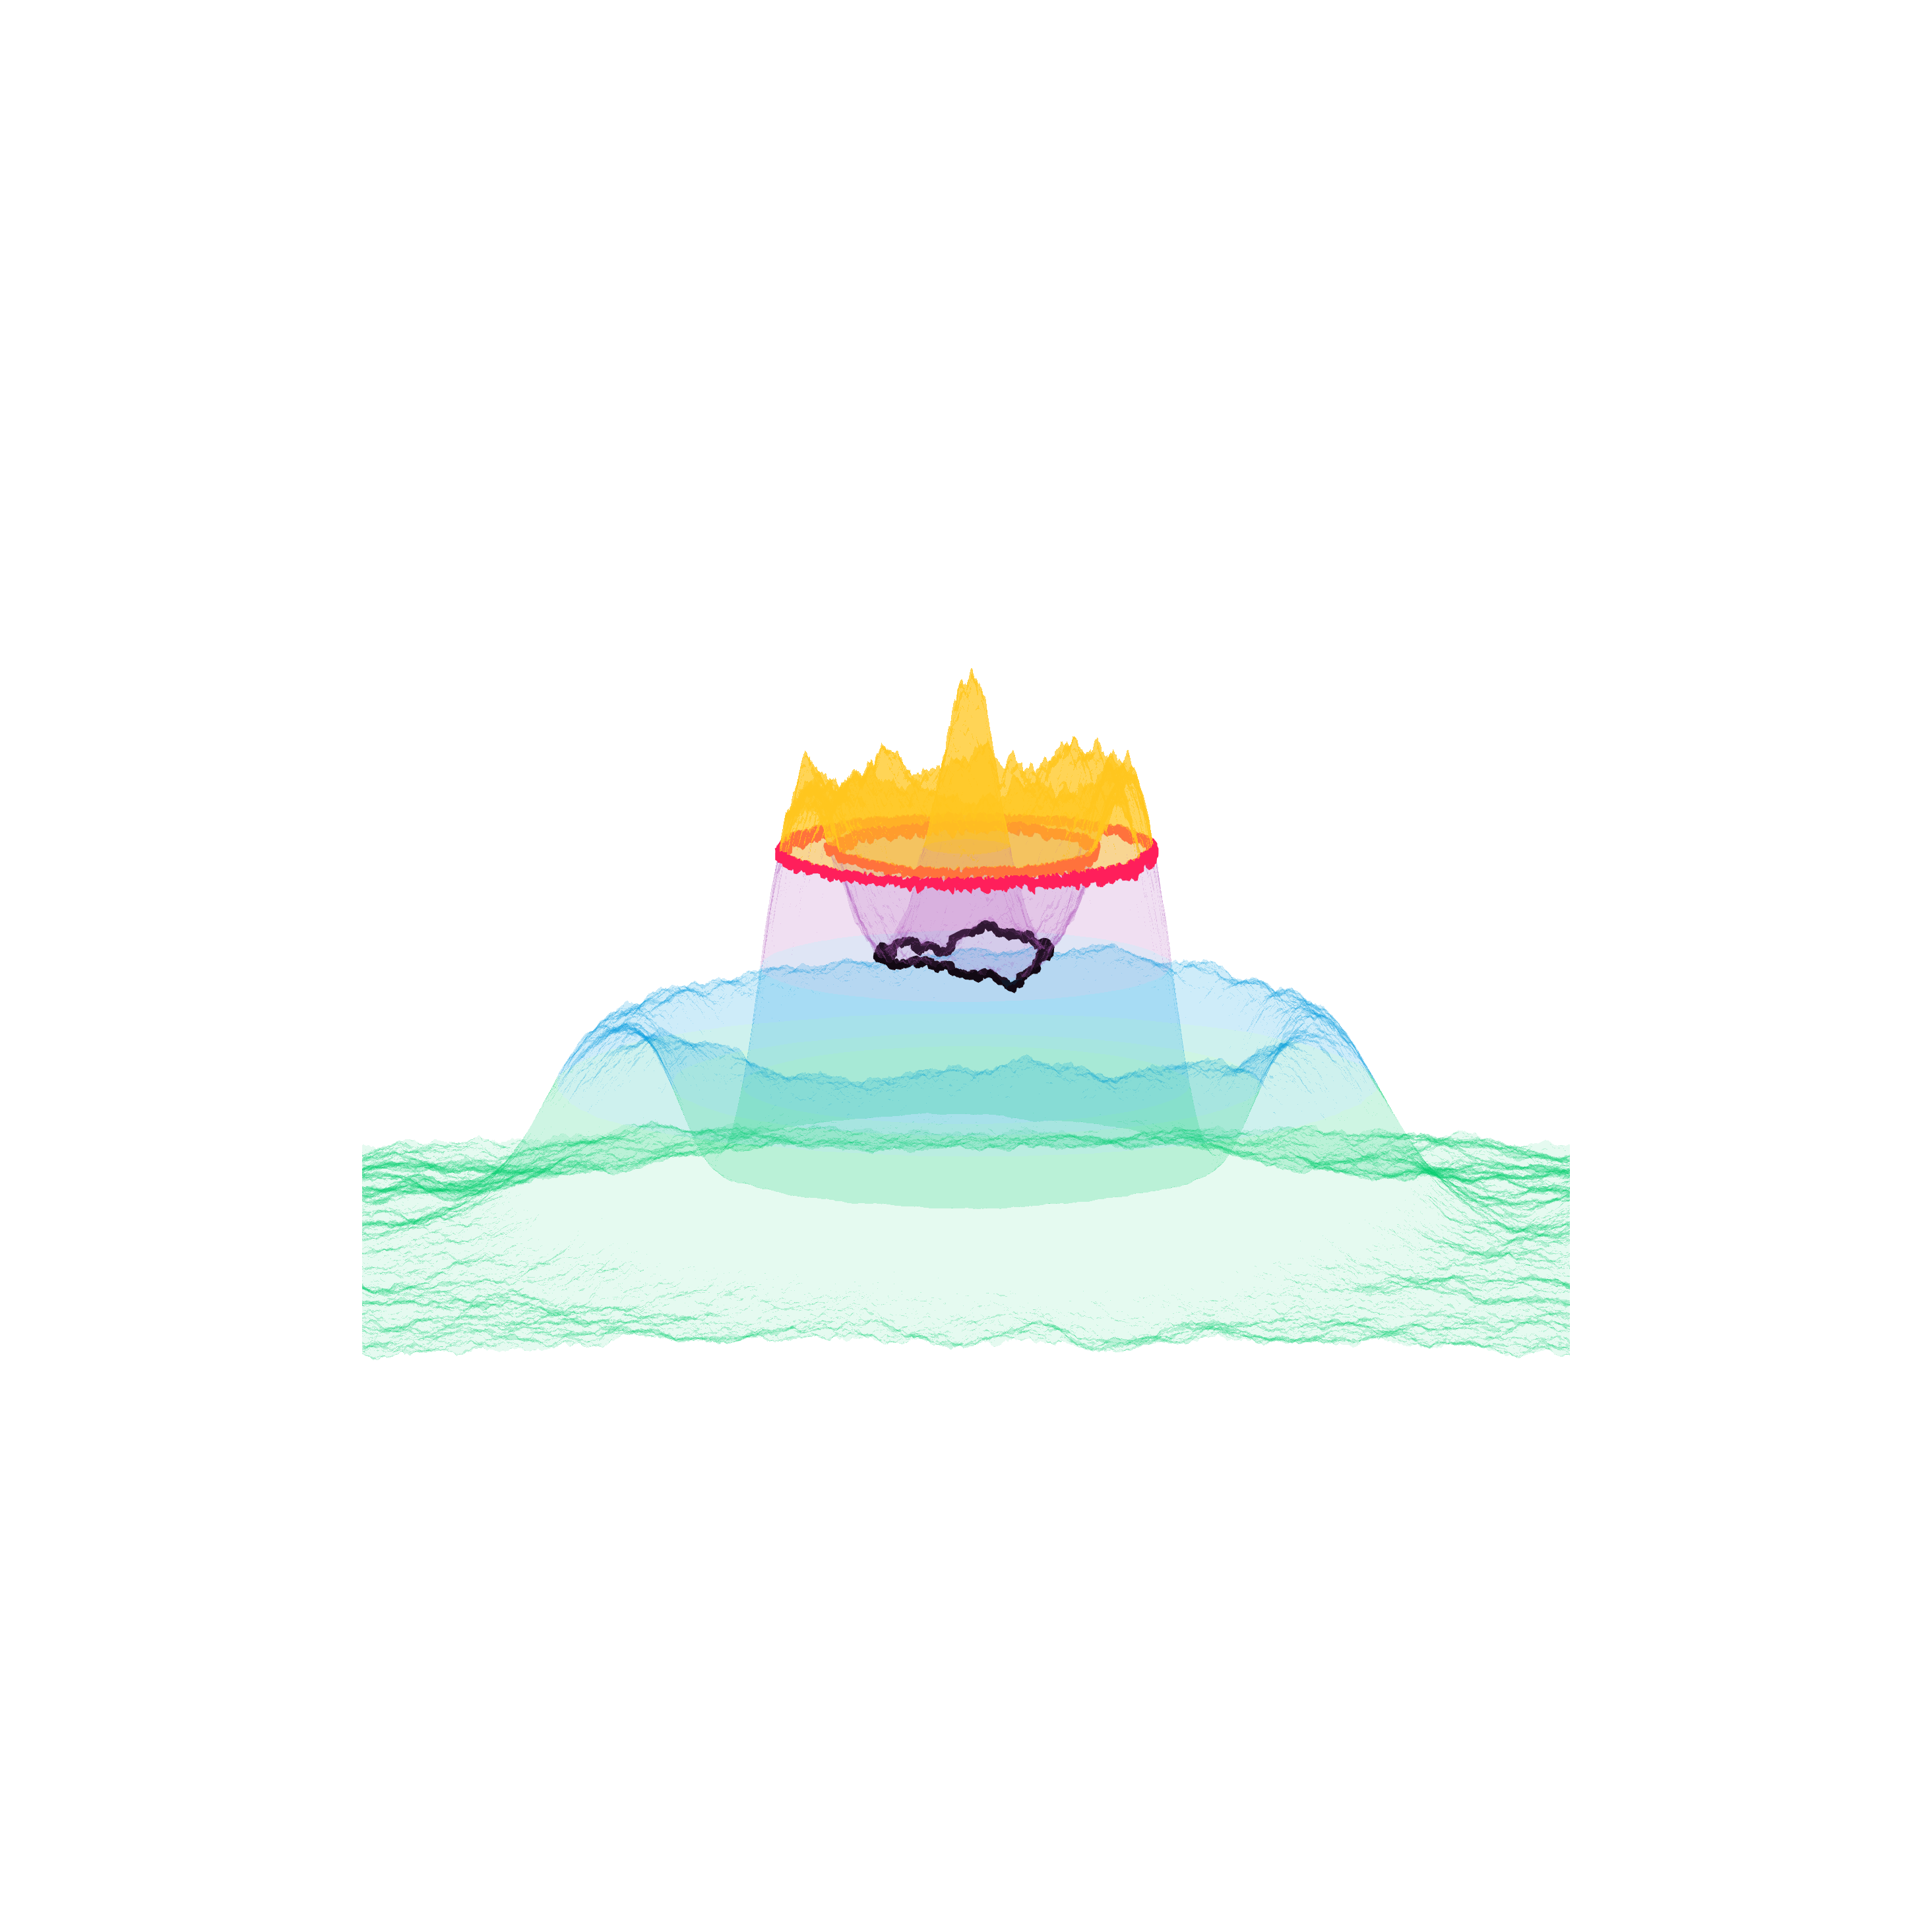
\includegraphics[trim=500 800 500 800, clip, width=0.24\textwidth]{scripts/figures/matching2/surf_side-2_0.png}
  % 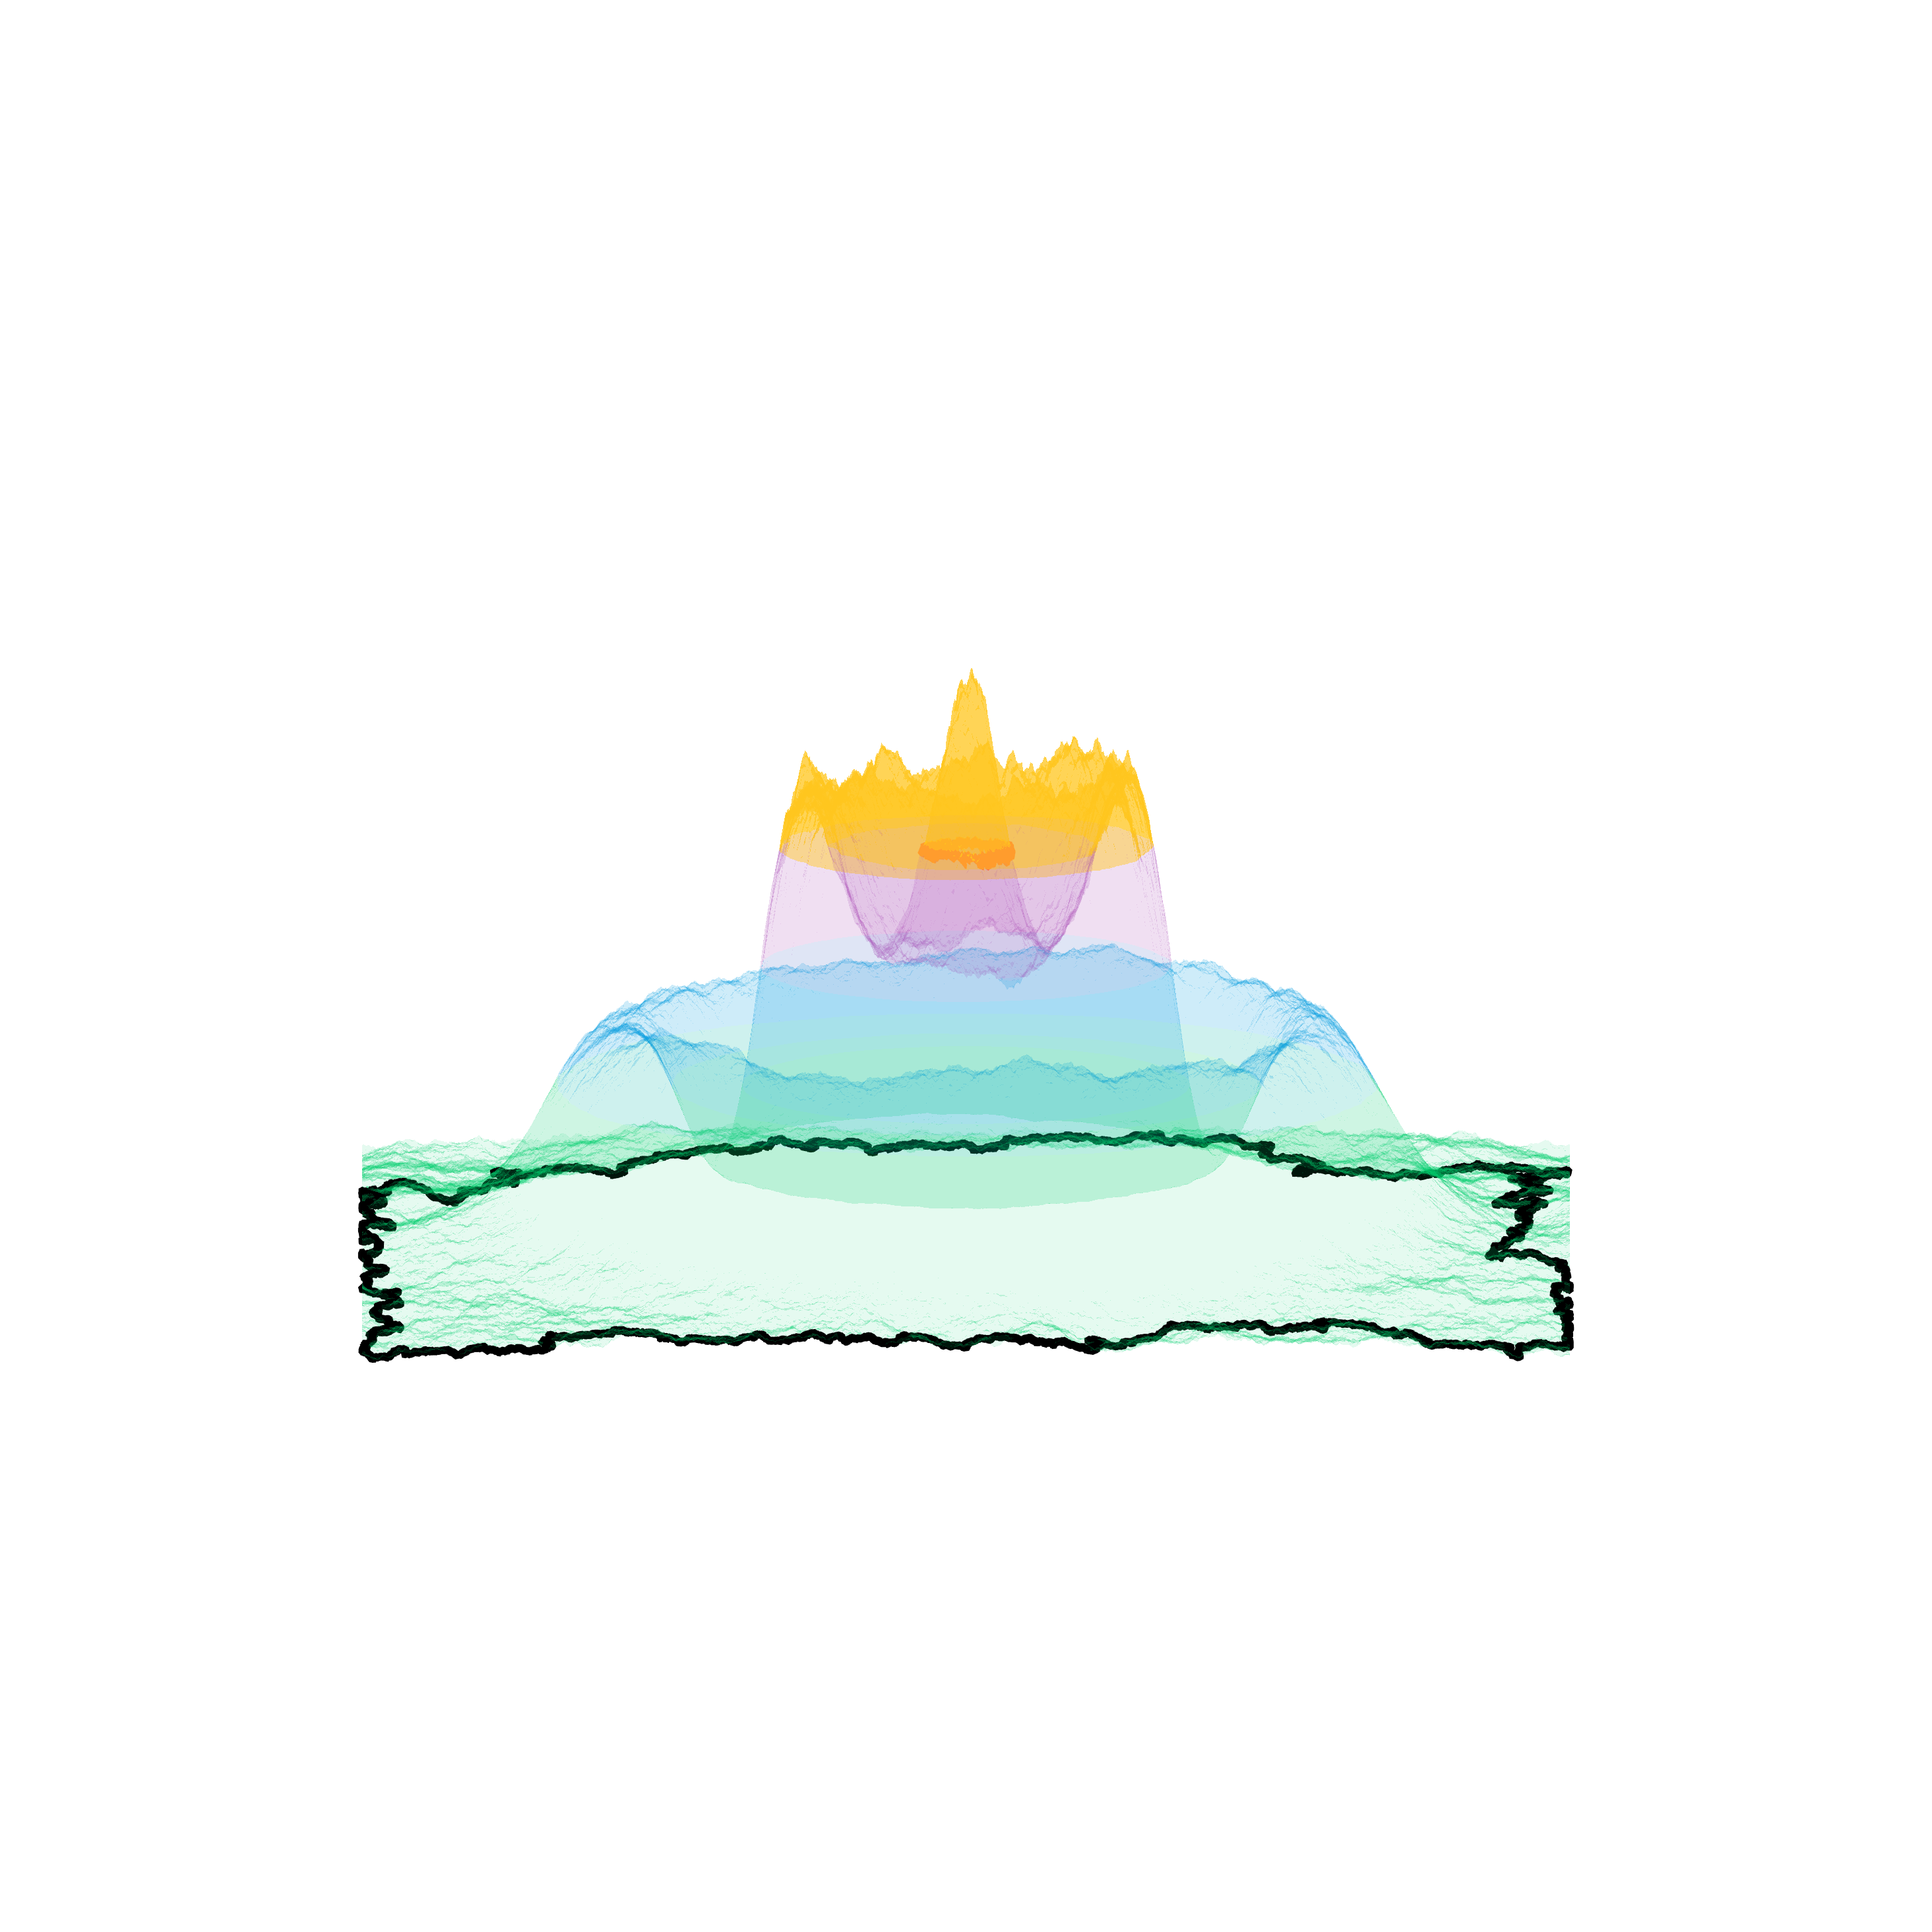
\includegraphics[trim=500 800 500 800, clip, width=0.24\textwidth]{scripts/figures/matching2/surf_side-2_1.png}
  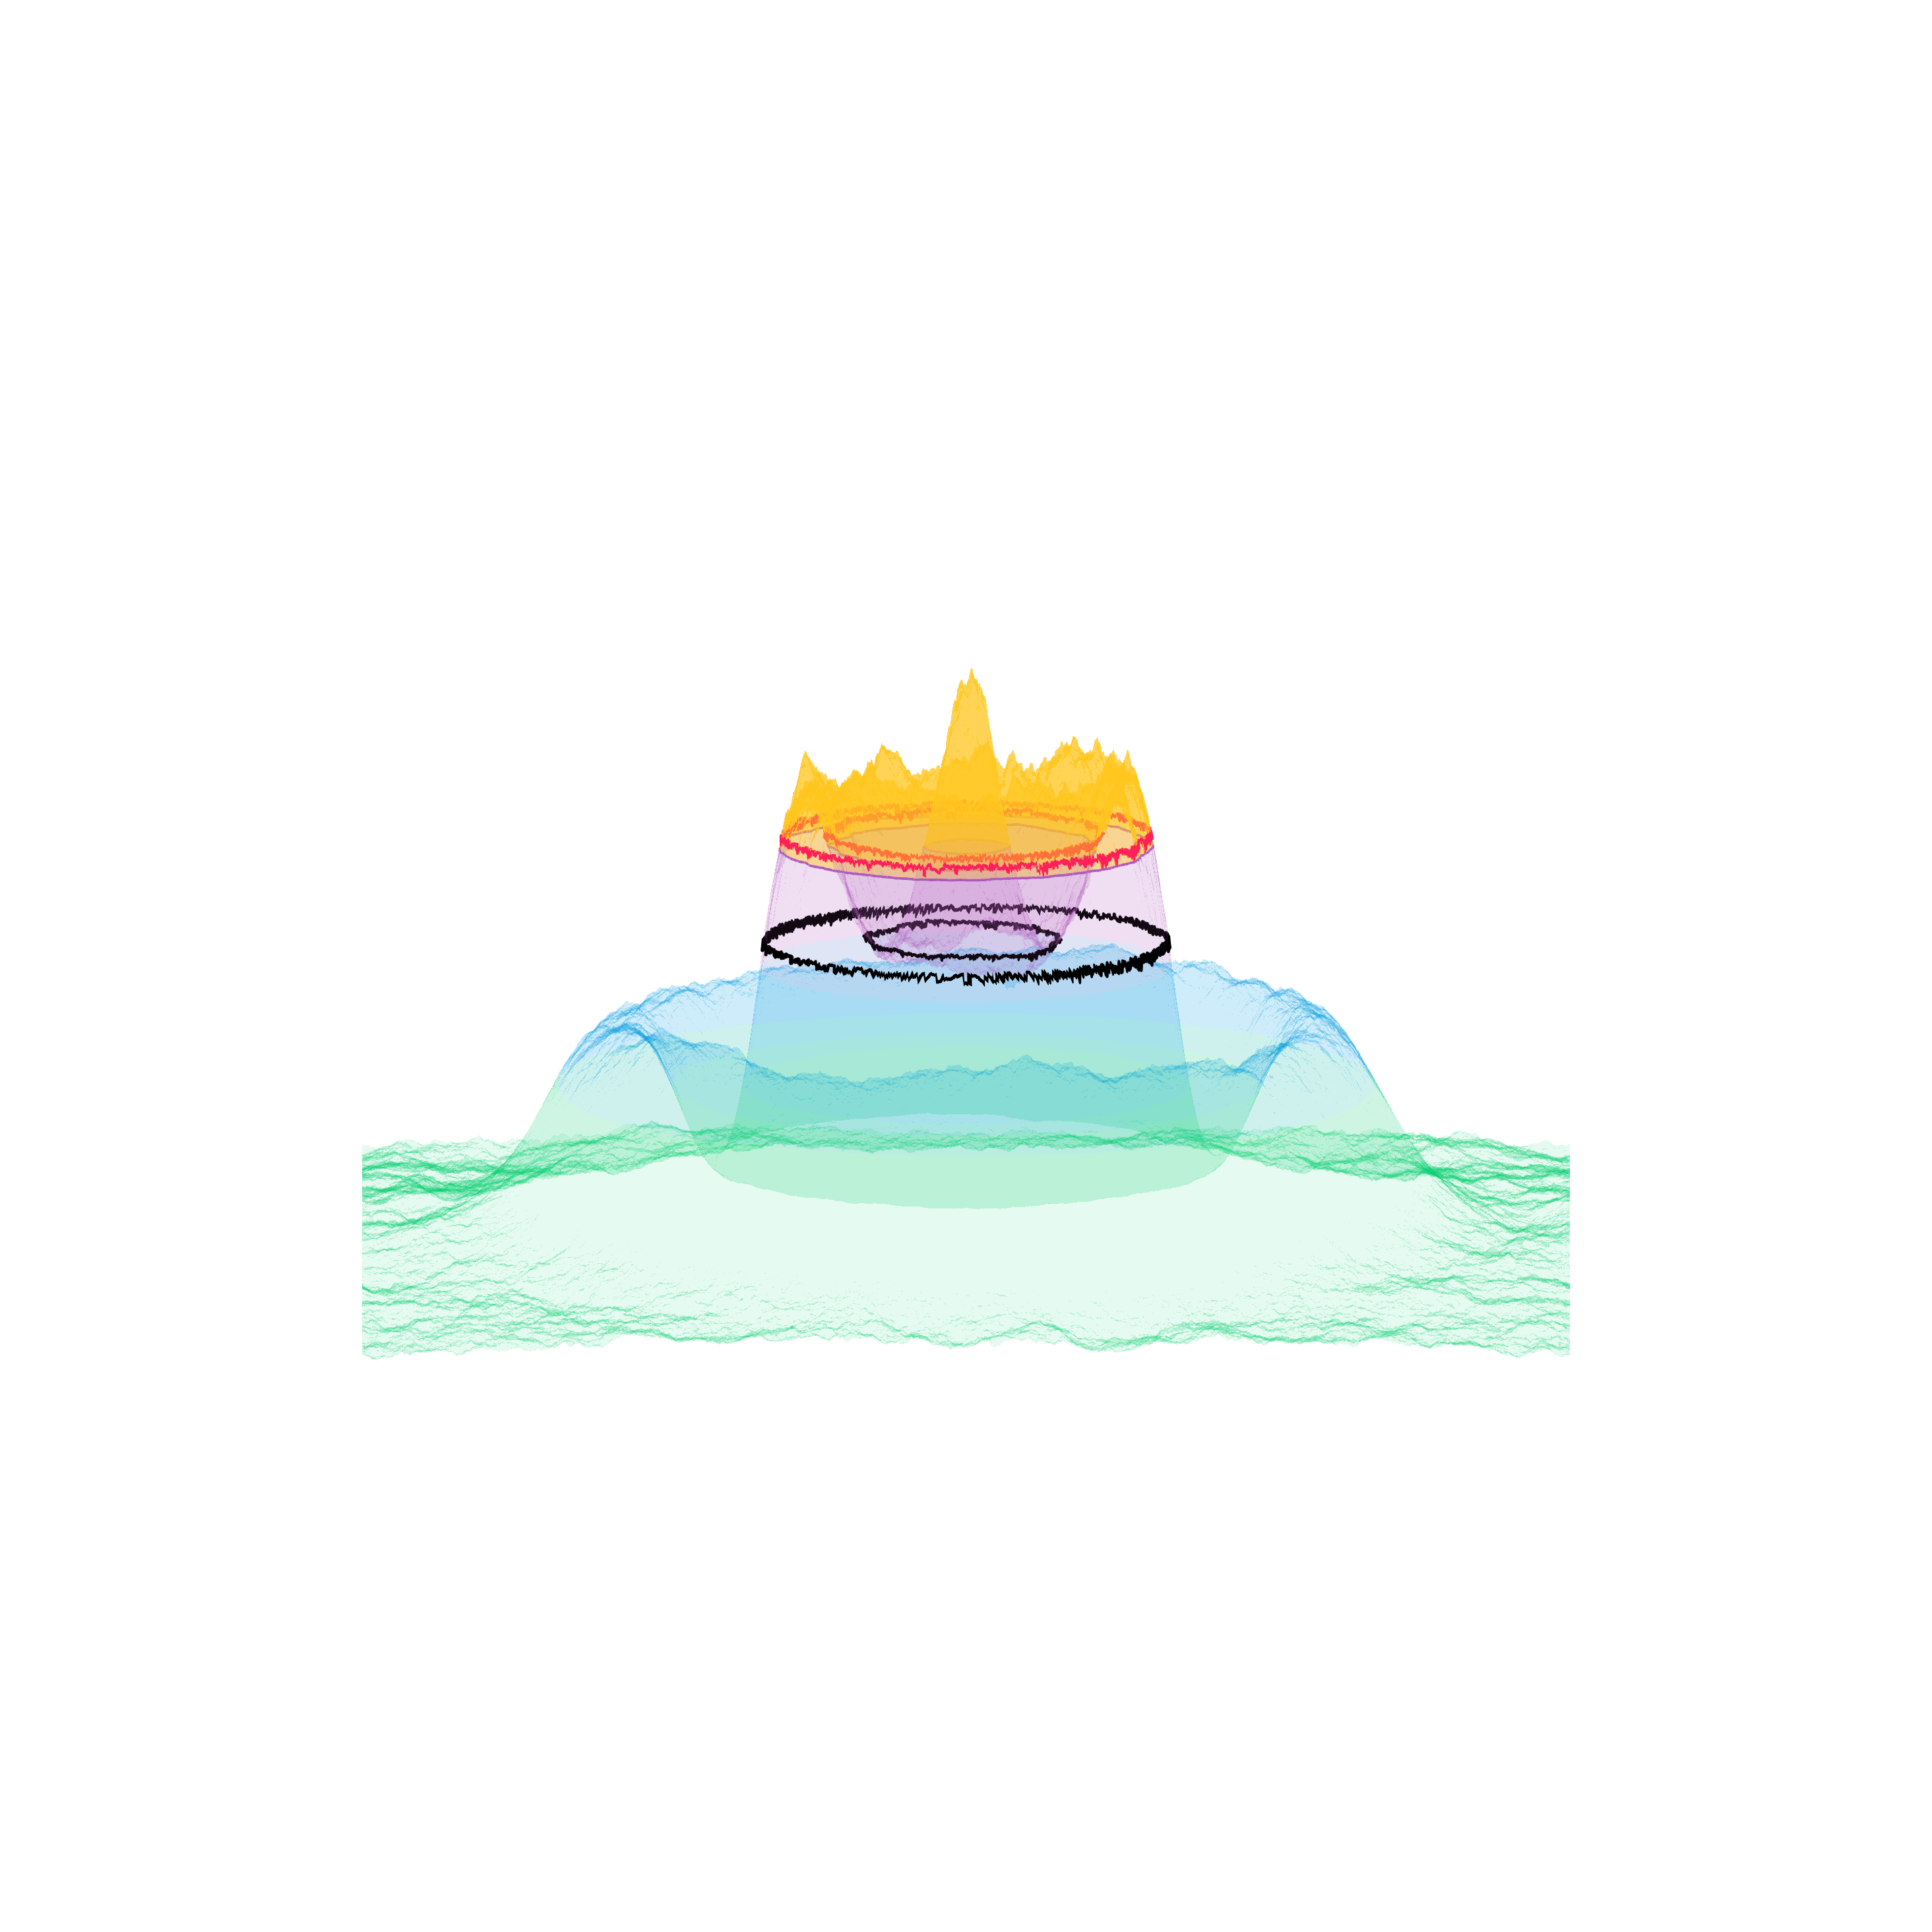
\includegraphics[trim=500 800 500 800, clip, width=0.3\textwidth]{scripts/figures/matching2/surf_side-2_2.png}\\
  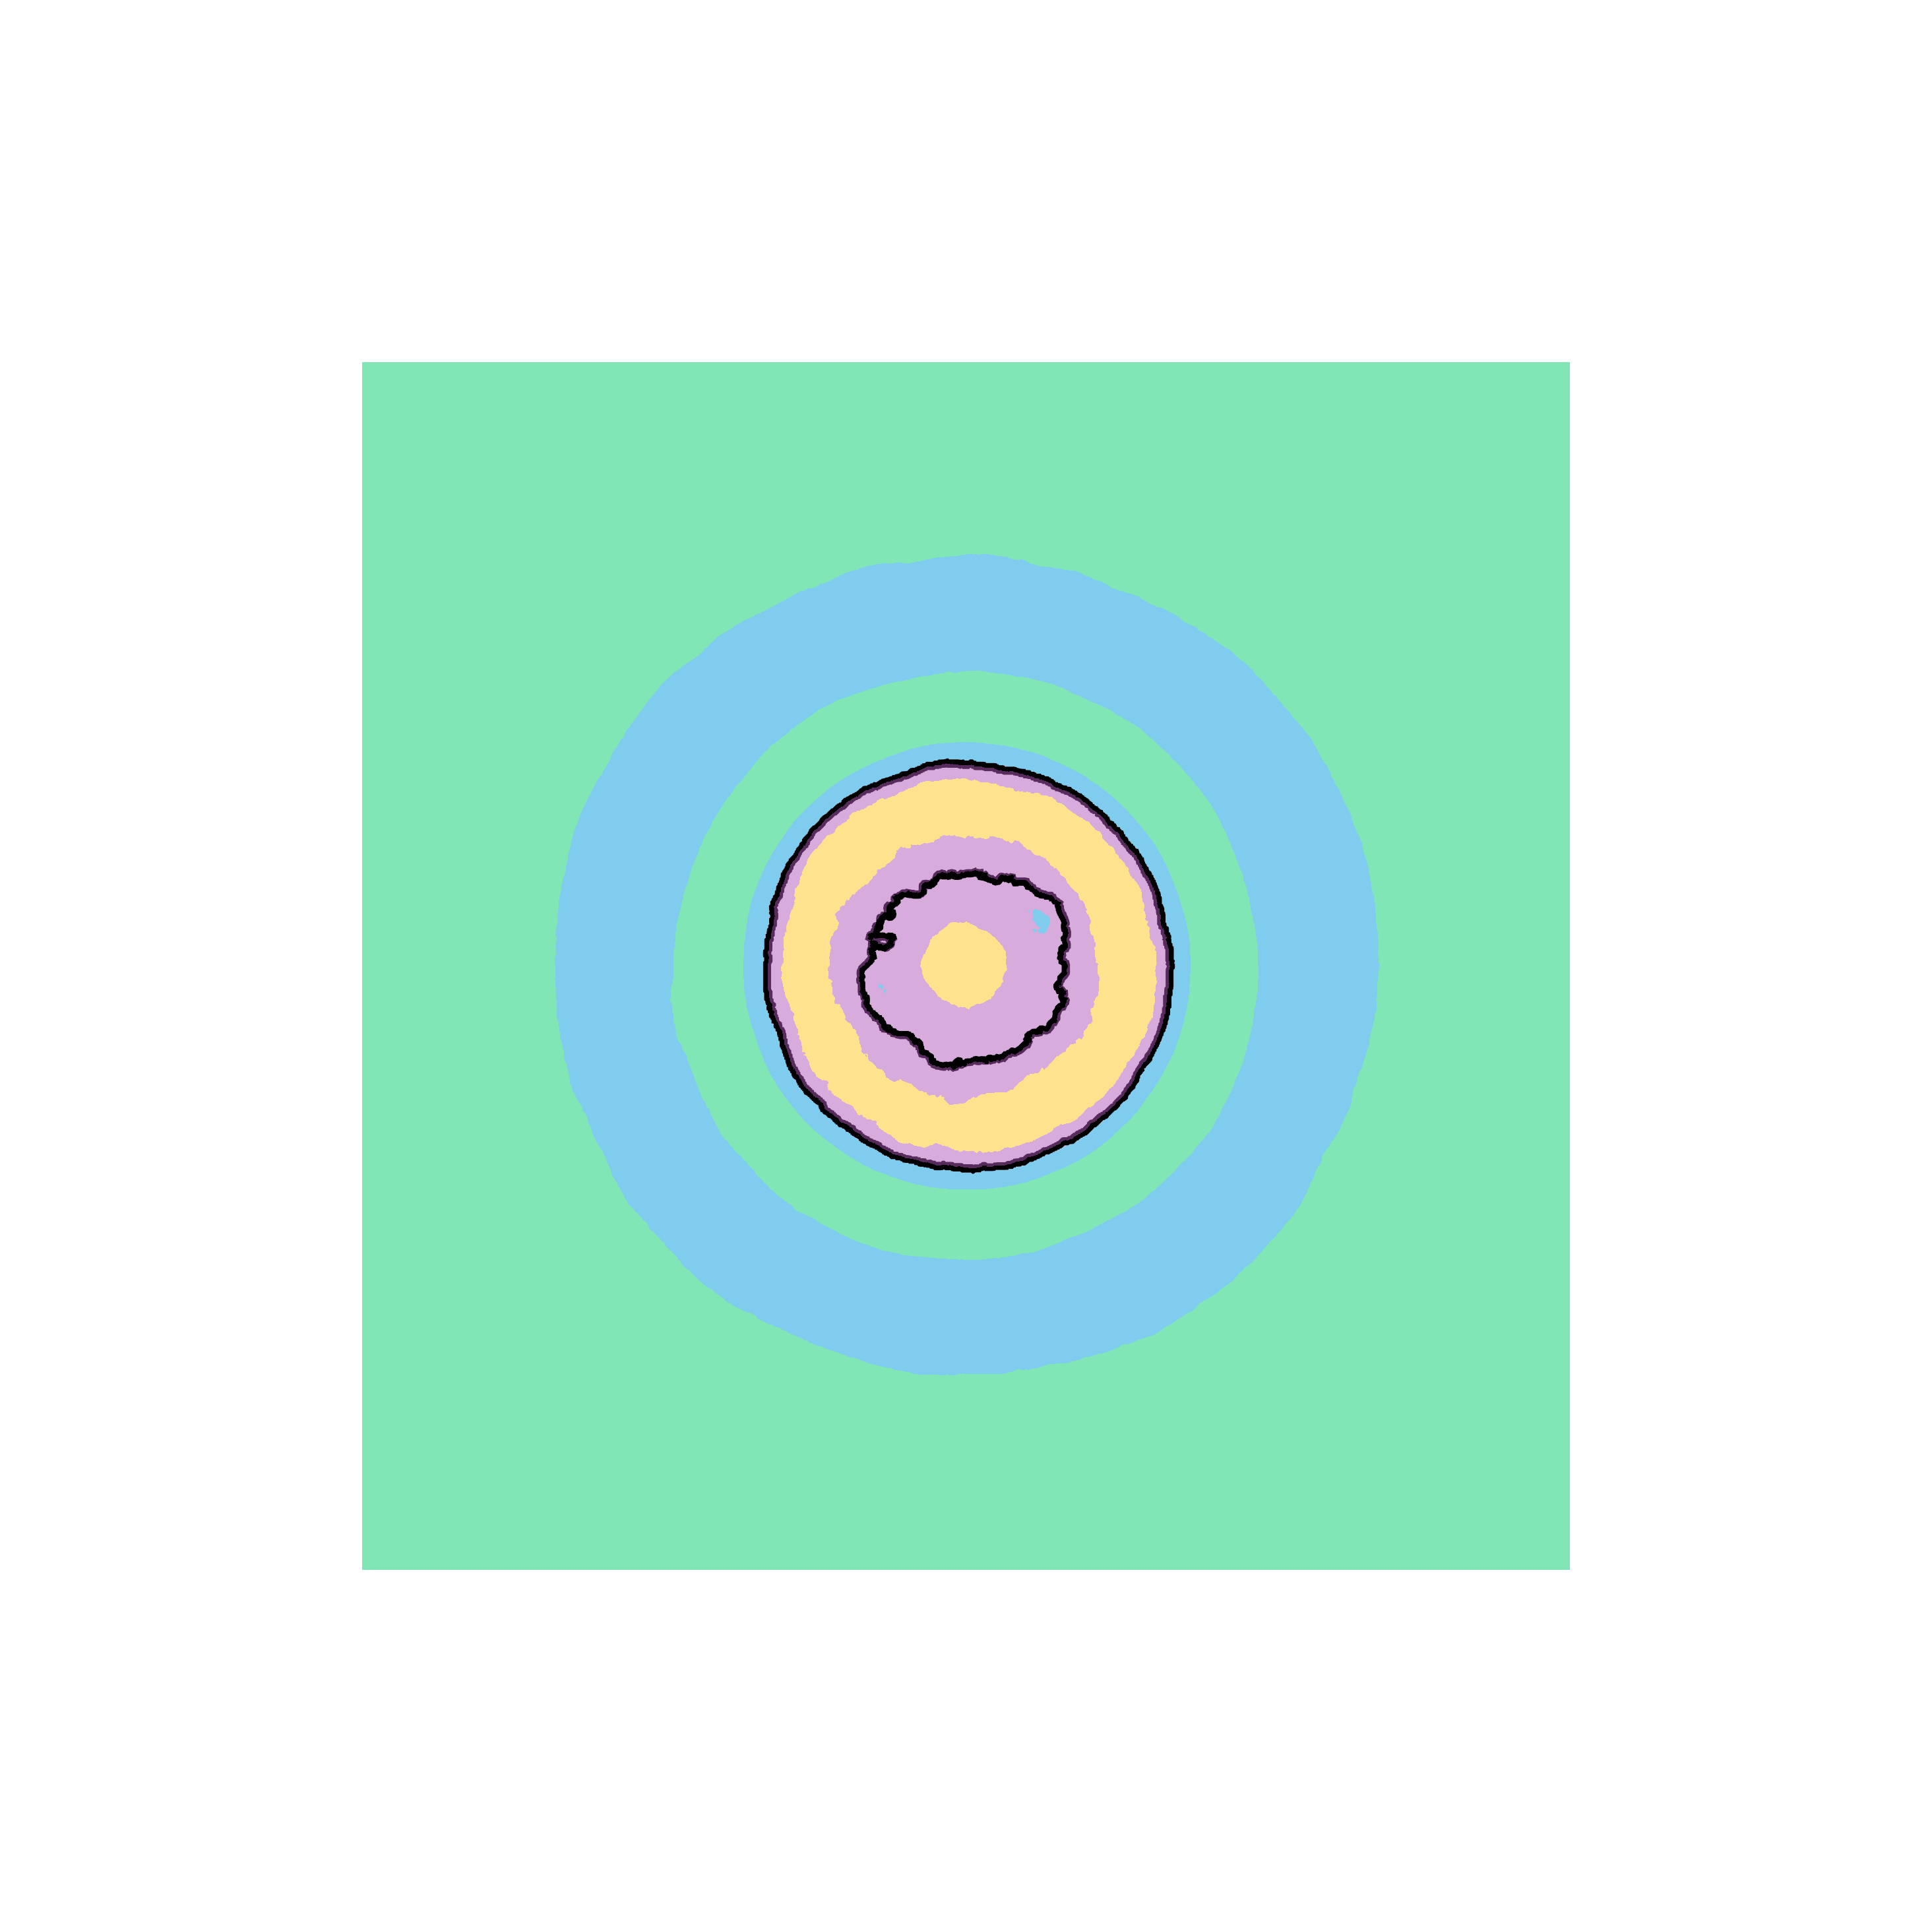
\includegraphics[trim=500 500 500 500, clip, width=0.3\textwidth]{scripts/figures/matching2/surf_top-2.png}
  % 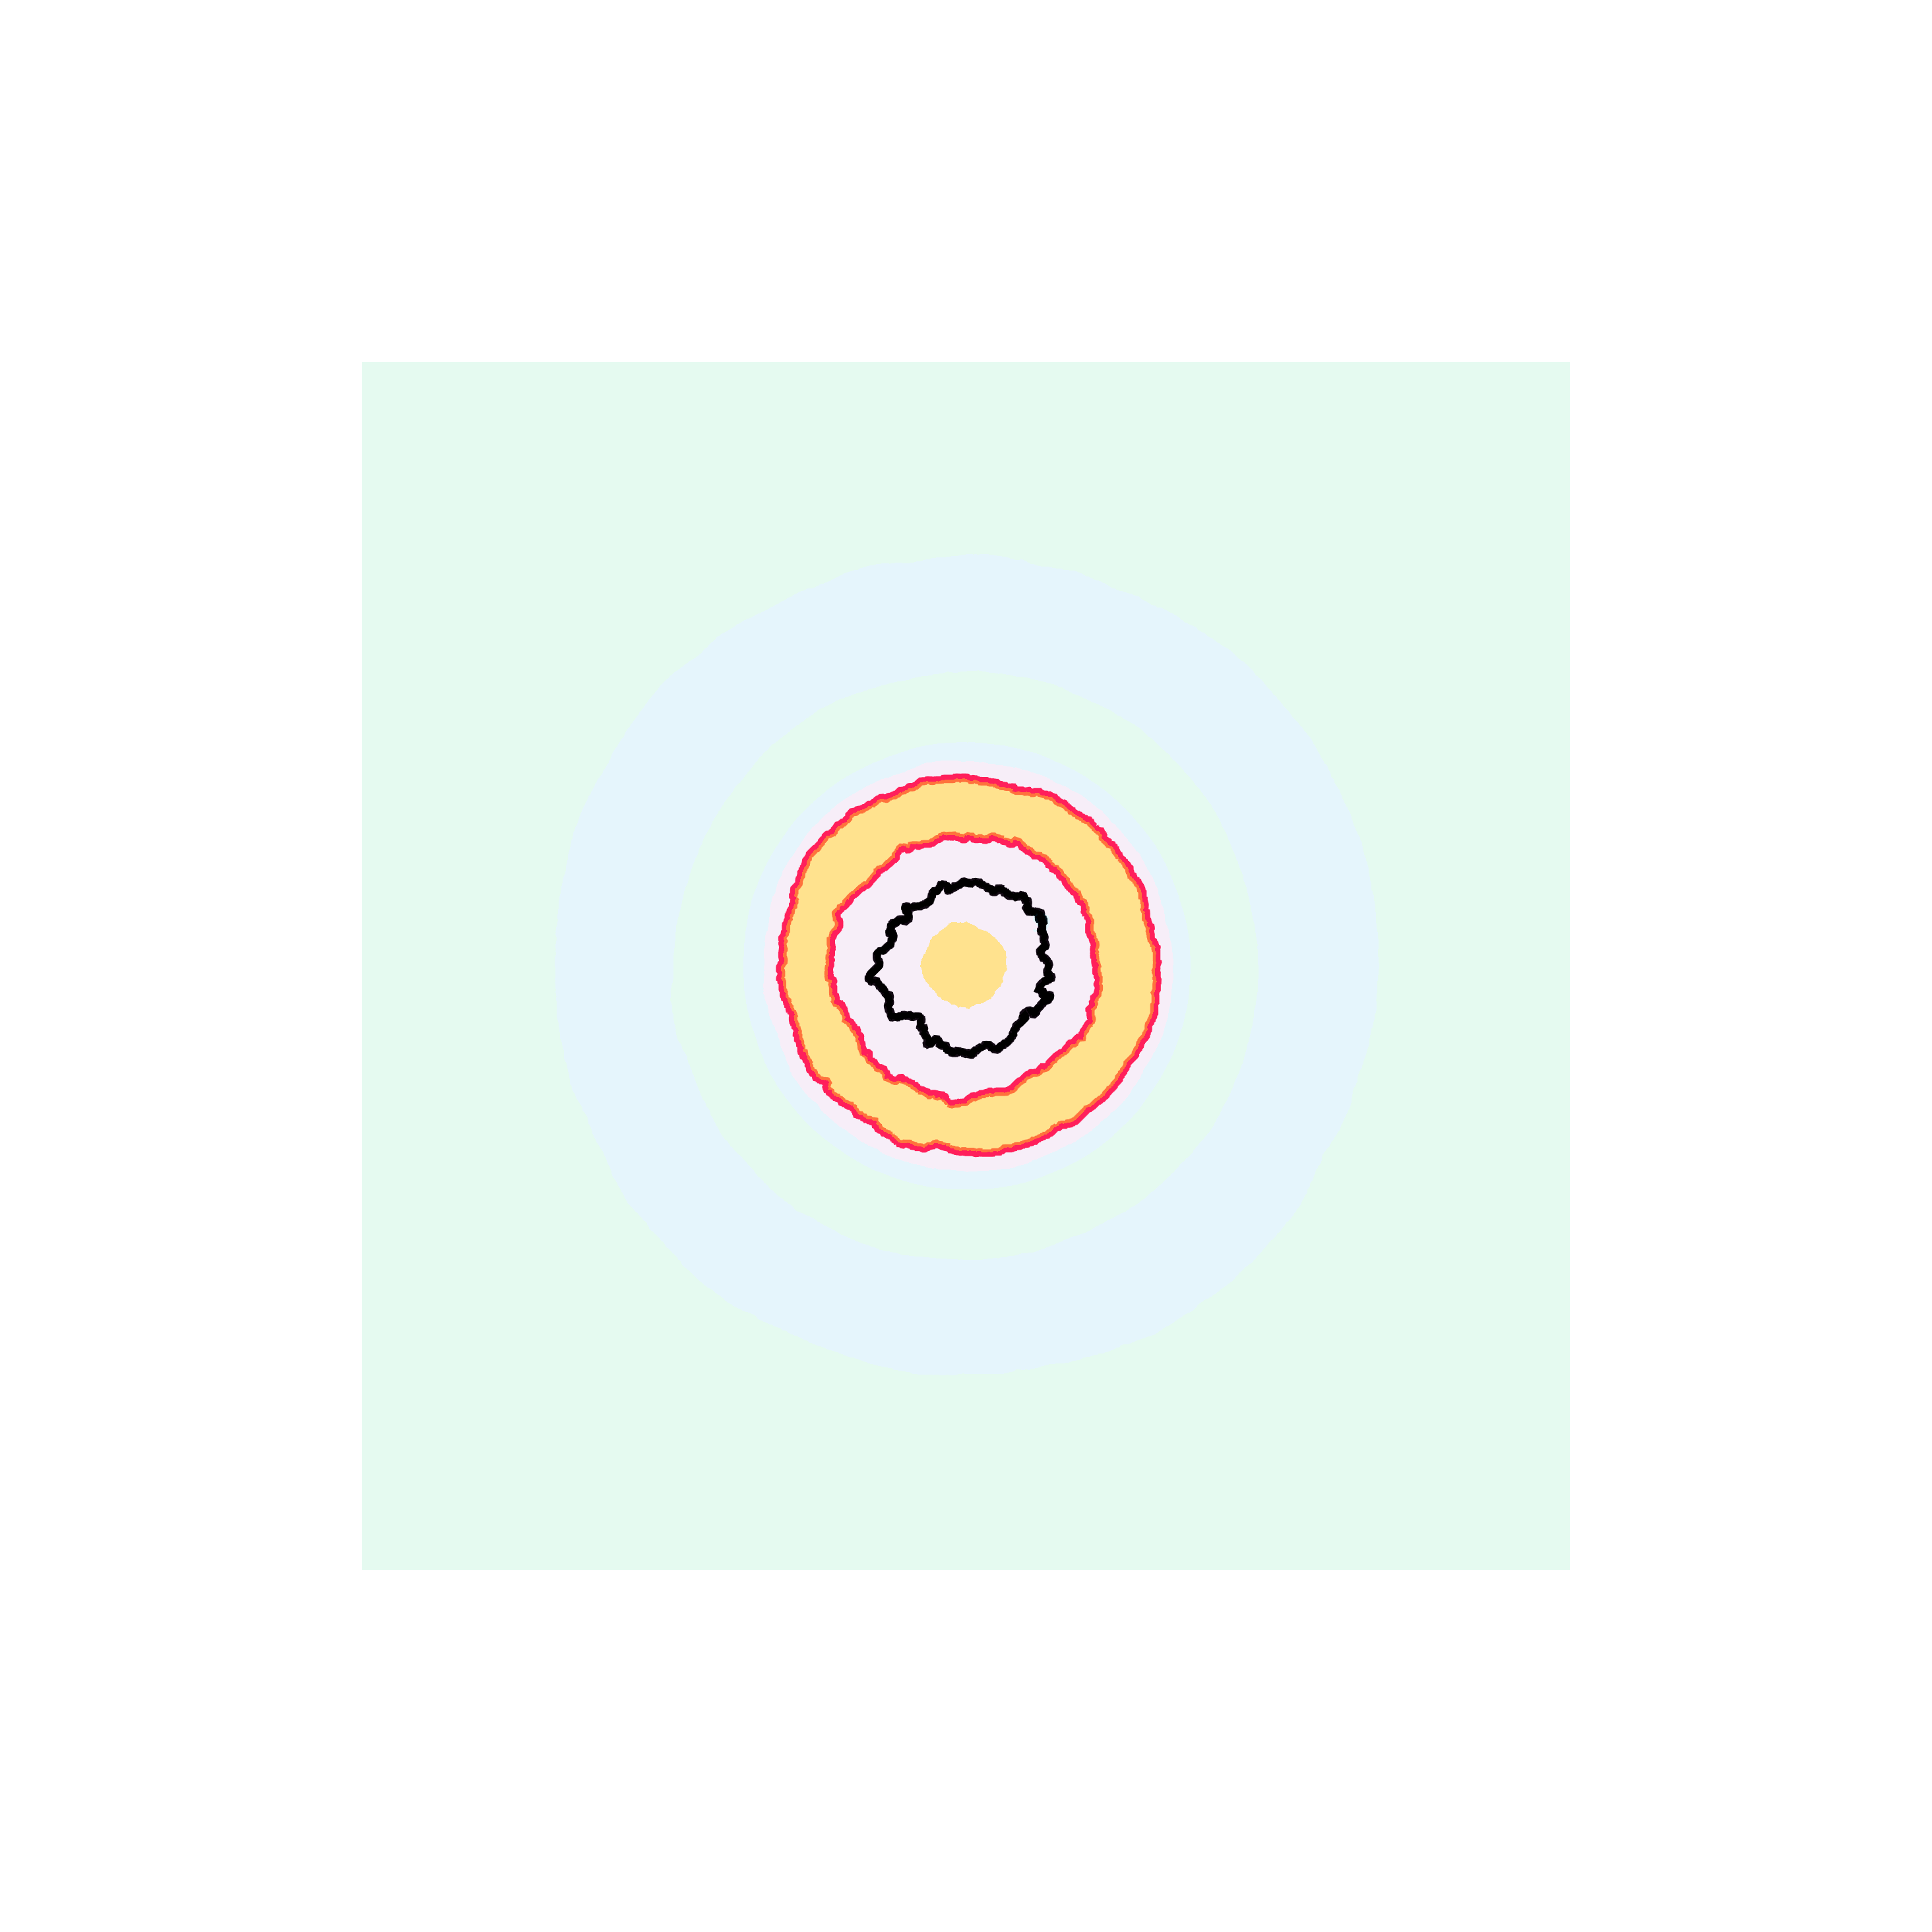
\includegraphics[trim=500 500 500 500, clip, width=0.24\textwidth]{scripts/figures/matching2/surf_top-2_0.png}
  % 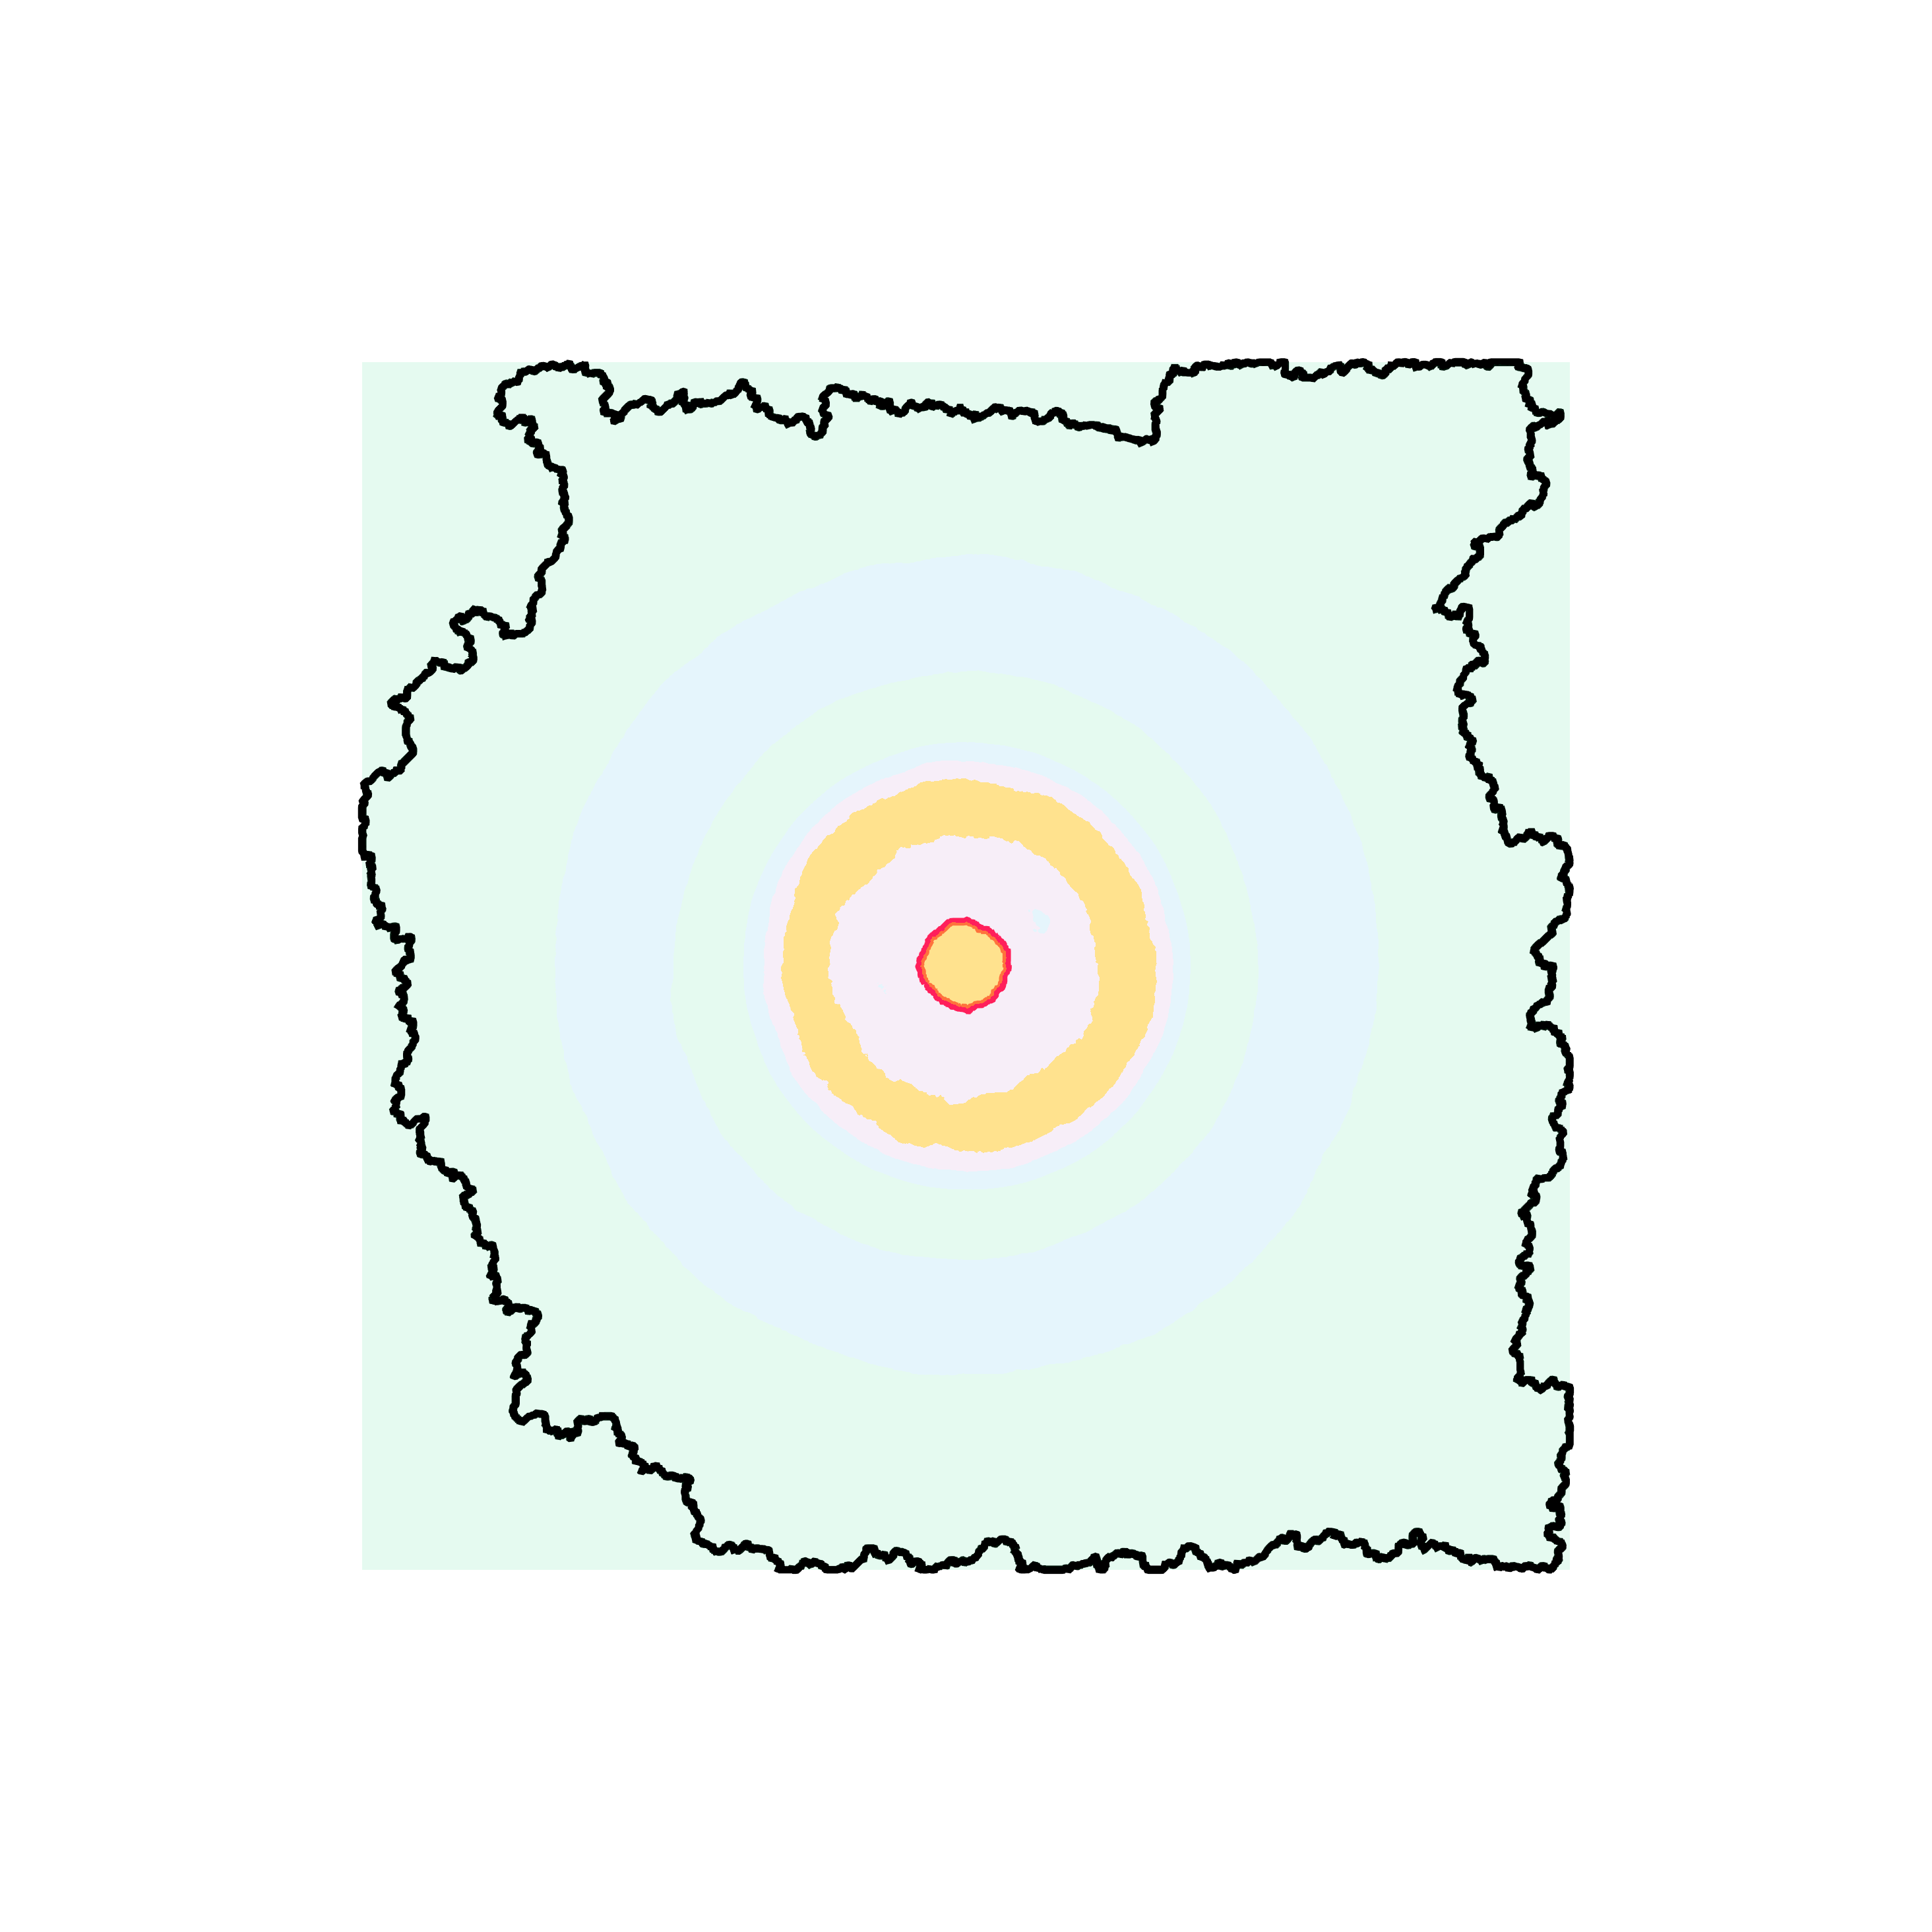
\includegraphics[trim=500 500 500 500, clip, width=0.24\textwidth]{scripts/figures/matching2/surf_top-2_1.png}
  \includegraphics[trim=500 500 500 500, clip, width=0.3\textwidth]{scripts/figures/matching2/surf_top-2_2.png}
\end{figure}

\begin{figure}[htbp]
  \centering
  \includegraphics[width=\textwidth]{scripts/figures/relative/dgm-1_0.png}
  \includegraphics[trim=500 800 500 800, clip, width=0.4\textwidth]{scripts/figures/relative/surf_side-1_0.png}
  \includegraphics[trim=500 500 500 500, clip, width=0.4\textwidth]{scripts/figures/relative/surf_top-1_0.png}
\end{figure}

\begin{figure}[htbp]
  \centering
  \includegraphics[width=\textwidth]{scripts/figures/relative/dgm-2_0.png}
  \includegraphics[trim=500 800 500 800, clip, width=0.4\textwidth]{scripts/figures/relative/surf_side-2_0.png}
  \includegraphics[trim=500 500 500 500, clip, width=0.4\textwidth]{scripts/figures/relative/surf_top-2_0.png}
\end{figure}

\begin{figure}[htbp]
  \centering
  \includegraphics[width=\textwidth]{scripts/figures/relative/dgm-2_1.png}
  \includegraphics[trim=500 800 500 800, clip, width=0.4\textwidth]{scripts/figures/relative/surf_side-2_1.png}
  \includegraphics[trim=500 500 500 500, clip, width=0.4\textwidth]{scripts/figures/relative/surf_top-2_1.png}
\end{figure}


% \section{Helpful Stuff}
% % !TeX root = ../../main.tex

\subsection{Some Helpful Lemmas}

% \begin{lemma}[Splitting Lemma (Hatcher p. 147)]\label{lem:splitting}
%   For a short exact sequence \[0\to A\xrightarrow{i} B\xrightarrow{j} C\to 0\] of abelian groups the following statements are equivalent
%   \begin{enumerate}
%     \item There is a homomorphism $p: B\to A$ such that $p\circ i = \mathbf{Id}_A$.
%     \item There is a homomorphism $s: C\to B$ such that $j\circ s = \mathbf{Id}_C$.
%     \item There is an isomorphism $B\cong A\oplus C$ making the commutative diagram below, where the maps in the lower row are the obvious ones $a\mapsto (a, 0)$ and $(a,c)\mapsto c$.
%
%     \[\begin{tikzcd}[column sep=small, row sep=small]
%               &                       & B\ar[dd, "\cong"]\ar[dr,"j"]  &         & \\
%       0\ar[r] & A\ar[ur, "i"]\ar[dr]  &                               & C\ar[r] & 0\\
%               &                       & A\oplus C\ar[ur]              &         &
%     \end{tikzcd}\]
%   \end{enumerate}
% \end{lemma}

\begin{lemma}[\textbf{The Five-Lemma} (Hatcher p. 129)]\label{lem:five}
  In a commutative diagram of abelian groups as below, if the two rows are exact and $\alpha,\beta,\delta$, and $\e$ are isomorphisms then $\gamma$ is an isomorphism.
  \[\begin{tikzcd}
      A\ar[r, "i"]\ar[d, "\alpha"]
    & B\ar[r, "j"]\ar[d, "\beta"]
    & C\ar[r, "k"]\ar[d, "\gamma"]
    & D\ar[r, "\ell"]\ar[d, "\delta"]
    & E\ar[d, "\e"]\\
    %
      A'\ar[r, "i'"]
    & B'\ar[r, "j'"]
    & C'\ar[r, "k'"]
    & D'\ar[r, "\ell'"]
    & E'\\
  \end{tikzcd}\]

  \begin{itemize}
    \item If $\beta$ and $\delta$ are surjective and $\e$ is injective then $\gamma$ is surjective.
    \item If $\beta$ and $\delta$ are injective and $\alpha$ is surjective then $\gamma$ is injective.
  \end{itemize}
\end{lemma}

\begin{theorem}[\textbf{Universal Coefficient Theorem} (Munkres p. 323, Corollary 53.2)]\label{thm:univ_coef}
  Let $(A,B)$ be a topological pair.
  Then for all $k$ and any abelian group $G$ there is a natural exact sequence
  \[ 0\to\mathrm{Ext}(\hom_{k-1}(A, B), G)\to \hom^k(A, B; G)\xrightarrow{\nu} \Hom(\hom_k(A, B), G)\to 0.\]
  This sequence splits, but not naturally.
\end{theorem}

\subsection{A Helpful Diagram}

% \begin{landscape}
% \begin{scriptsize}
% \begin{centering}
% \[\begin{tikzcd}[row sep=large, column sep=scriptsize]
%   |[alias=U]| \D{\omega-c(\delta+\zeta)}{\alpha-3c\delta}
%                                   \arrow[to=V, "\gamma_{\alpha-3c\delta}{[3c\delta]}"]
%                                   \arrow[to=Sa, "f_{\omega-c(\delta+\zeta}{[\alpha-3c\delta]}"]
%   &&&& |[alias=V]| \D{\omega}{\alpha}
%                                   \arrow[to=W, "\pi_\alpha{[3c\zeta]}"]
%                                   \arrow[to=Ta, "f_\omega{[\alpha]}"]
%   &&&& |[alias=W]|
%   \D{\omega+c(\delta+2\zeta)}{\alpha+3c\zeta}\\
%   %
%   & |[alias=Sa]|
%   \P{\omega-c\zeta}{\delta}{\alpha-2c\delta}
%                                   \arrow[to=Sb, "s_{\alpha-2c\delta}"]
%                                   \arrow[to=CSa, "(\E\N_{w-c\zeta}^\delta{[\alpha-2c\delta]})^{-1}"]
%   && |[alias=Sb]| \P{\omega-c\zeta}{2\delta}{\alpha-2c\delta}
%                                   \arrow[to=Ta, "\vartheta_{\alpha-2c\delta}{[2c\delta+\zeta]}"]
%                                   \arrow[to=V, "m_{\omega-c\zeta}^{2\delta}{[\alpha-2c\delta]}"]
%   && |[alias=Ta]| \P{\omega+c\delta}{\zeta}{\alpha+c\zeta}
%                                   \arrow[to=Tb, "t_{\alpha+c\zeta}"]
%                                   \arrow[to=CTa, "(\E\N_{w+c\delta}^\zeta{[\alpha+c\zeta]})^{-1}"]
%   && |[alias=Tb]| \P{\omega+c\delta}{2\zeta}{\alpha+c\zeta}
%                                   \arrow[to=W, "m_{\omega+c\delta}^{2\zeta}{[\alpha+c\zeta]}"]
%   &\\
%   %
%   & |[alias=CSa]|
%   \CP{\omega-c\zeta}{\delta}{\alpha-2c\delta}
%                                   \arrow[to=CSb, "\check{s}_{\alpha-2c\delta}"]
%                                   \arrow[to=RS, "\I_{\omega-c\zeta}^\delta{[\alpha-2c\delta]}"']
%   && |[alias=CSb]| \CP{\omega-c\zeta}{2\delta}{\alpha-2c\delta}
%                                   \arrow[to=Sb, "\E\N_{w-c\zeta}^{2\delta}{[\alpha-2c\delta]}"]
%                                   \arrow[to=CTa, "\check{\vartheta}_{\alpha-2c\delta}{[2c\delta+\zeta]}"]
%   && |[alias=CTa]| \CP{\omega+c\delta}{\zeta}{\alpha+c\zeta}
%                                   \arrow[to=CTb, "\check{t}_{\alpha+c\zeta}"]
%                                   \arrow[to=RT, "\I_{\omega+c\delta}^\zeta{[\alpha+c\zeta]}"']
%   && |[alias=CTb]| \CP{\omega+c\delta}{2\zeta}{\alpha+c\zeta}
%                                   \arrow[to=Tb, "\E\N_{w+c\delta}^{2\zeta}{[\alpha+2c\zeta]}"]
%   &\\
%   %
%   && |[alias=RS]| \CP{\omega-c\zeta}{2\delta}{\alpha-2c\delta}
%                                   \arrow[to=CSb, "\J_{\omega-c\zeta}^{2\delta}{[\alpha-2c\delta]}"]
%                                   \arrow[to=RT, "\rips\lambda_{\alpha-c\zeta}{[c(2\delta+\zeta)]}"]
%   &&&& |[alias=RT]| \RP{\omega+c\delta}{2\zeta}{\alpha+c\zeta}
%                                   \arrow[to=CTb, "\J_{\omega+c\delta}^{2\zeta}{[\alpha+c\zeta]}"]
%   &&\\
% \end{tikzcd}\]
% \end{centering}
% \end{scriptsize}
% \end{landscape}

\begin{scriptsize}
\begin{centering}
\[\begin{tikzcd}[row sep=large, column sep=scriptsize]
  |[alias=U]| \DD{\omega-c(\delta+\zeta)}
                                  \arrow[to=V, two heads, blue, "\Gamma{[3c\delta]}"]
                                  \arrow[to=Sa,blue, "F"]
  &&&& |[alias=V]| \DD{\omega}
                                  \arrow[to=W, hook,red, "\Pi{[3c\zeta]}"]
                                  \arrow[to=Ta,red, "G"]
  &&&& |[alias=W]|
  \DD{\omega+c(\delta+2\zeta)}\\
  %
  & |[alias=Sa]|
  \E\PP{\omega-c\zeta}{\delta}
                                  \arrow[to=Sb, blue, "\mathcal{S}"]
                                  \arrow[to=CSa, "(\E\N_{w-c\zeta}^\delta)^{-1}"]
  && |[alias=Sb]| \E\PP{\omega-c\zeta}{2\delta}
                                  \arrow[to=Ta, "\Theta{[2c\delta+\zeta]}"]
                                  \arrow[to=V, blue, "M"]
  && |[alias=Ta]| \E\PP{\omega+c\delta}{\zeta}
                                  \arrow[to=Tb, red, "\mathcal{T}"]
                                  \arrow[to=CTa, "(\E\N_{w+c\delta}^\zeta)^{-1}"]
  && |[alias=Tb]| \E\PP{\omega+c\delta}{2\zeta}
                                  \arrow[to=W, red, "N"]
  &\\
  %
  & |[alias=CSa]|
  \CPP{\omega-c\zeta}{\delta}
                                  \arrow[to=CSb, green, "\cech\mathcal{S}"]
                                  \arrow[to=RS, green, "\I_{\omega-c\zeta}^\delta"']
  && |[alias=CSb]| \CPP{\omega-c\zeta}{2\delta}
                                  \arrow[to=Sb, "\E\N_{w-c\zeta}^{2\delta}"]
                                  \arrow[to=CTa, "\cech\Theta{[2c\delta+c\zeta]}"]
  && |[alias=CTa]| \CPP{\omega+c\delta}{\zeta}
                                  \arrow[to=CTb, orange, "\cech\mathcal{T}"]
                                  \arrow[to=RT, orange, "\I_{\omega+c\delta}^\zeta"']
  && |[alias=CTb]| \CPP{\omega+c\delta}{2\zeta}
                                  \arrow[to=Tb, "\E\N_{w+c\delta}^{2\zeta}"]
  &\\
  %
  && |[alias=RS]| \RPP{\omega-c\zeta}{2\delta}
                                  \arrow[to=CSb, green, "\J_{\omega-c\zeta}^{2\delta}"]
                                  \arrow[to=RT, "\rips\Lambda"]
  &&&& |[alias=RT]| \RPP{\omega+c\delta}{2\zeta}
                                  \arrow[to=CTb, orange, "\J_{\omega+c\delta}^{2\zeta}"]
  &&\\
\end{tikzcd}\]
\end{centering}
\end{scriptsize}

\begin{enumerate}
  \item Blue commutes (all inclusions) + green commutes (all inclusions) + middle left square commutes with inclusion (pers. nerve lemma) $\implies$ weak interleaving of $\Gamma$ with $\RPP{\omega-c\zeta}{2\delta}$.
  \item Red commutes (all inclusions) + orange commutes (all inclusions) + middle right square commutes with inclusion (pers. nerve lemma) $\implies$ weak interleaving of $\Pi$ with $\RPP{\omega+c\delta}{2\zeta}$.
  \item Middle commutes using the same arguments $\implies$ weak interleaving of $\rips\Lambda$ with $\DD{\omega}$
  \item weak interleaving of $\Gamma$ with $\RPP{\omega-c\zeta}{2\delta}$ + weak interleaving of $\rips\Lambda$ with $\DD{\omega}$ + path \textbf{down} from $\Gamma$ to $\rips\Lambda$ is an image module homomorphism $\implies$ partial interleaving of image modules from $\Gamma$ to $\rips\Lambda$.
  \item weak interleaving of $\rips\Lambda$ with $\DD{\omega}$ + weak interleaving of $\Pi$ with $\RPP{\omega+c\delta}{2\zeta}$ + path \textbf{up} from $\rips\Lambda$ to $\Pi$ is an image module homomorphism $\implies$ partial interleaving of image modules from $\rips\Lambda$ to $\Pi$.
  \item these two partial interleavings + $\Gamma$ epi + $\Pi$ mono $\implies$ $\im~\rips\Lambda$ is interleaved with $\DD{\omega}$ by Lemma~\ref{thm:interleaving_main}.
\end{enumerate}


\end{document}
